\documentclass[twoside]{book}

% Packages required by doxygen
\usepackage{fixltx2e}
\usepackage{calc}
\usepackage{doxygen}
\usepackage[export]{adjustbox} % also loads graphicx
\usepackage{graphicx}
\usepackage[utf8]{inputenc}
\usepackage{makeidx}
\usepackage{multicol}
\usepackage{multirow}
\PassOptionsToPackage{warn}{textcomp}
\usepackage{textcomp}
\usepackage[nointegrals]{wasysym}
\usepackage[table]{xcolor}

% Font selection
\usepackage[T1]{fontenc}
\usepackage[scaled=.90]{helvet}
\usepackage{courier}
\usepackage{amssymb}
\usepackage{sectsty}
\renewcommand{\familydefault}{\sfdefault}
\allsectionsfont{%
  \fontseries{bc}\selectfont%
  \color{darkgray}%
}
\renewcommand{\DoxyLabelFont}{%
  \fontseries{bc}\selectfont%
  \color{darkgray}%
}
\newcommand{\+}{\discretionary{\mbox{\scriptsize$\hookleftarrow$}}{}{}}

% Page & text layout
\usepackage{geometry}
\geometry{%
  a4paper,%
  top=2.5cm,%
  bottom=2.5cm,%
  left=2.5cm,%
  right=2.5cm%
}
\tolerance=750
\hfuzz=15pt
\hbadness=750
\setlength{\emergencystretch}{15pt}
\setlength{\parindent}{0cm}
\setlength{\parskip}{0.2cm}
\makeatletter
\renewcommand{\paragraph}{%
  \@startsection{paragraph}{4}{0ex}{-1.0ex}{1.0ex}{%
    \normalfont\normalsize\bfseries\SS@parafont%
  }%
}
\renewcommand{\subparagraph}{%
  \@startsection{subparagraph}{5}{0ex}{-1.0ex}{1.0ex}{%
    \normalfont\normalsize\bfseries\SS@subparafont%
  }%
}
\makeatother

% Headers & footers
\usepackage{fancyhdr}
\pagestyle{fancyplain}
\fancyhead[LE]{\fancyplain{}{\bfseries\thepage}}
\fancyhead[CE]{\fancyplain{}{}}
\fancyhead[RE]{\fancyplain{}{\bfseries\leftmark}}
\fancyhead[LO]{\fancyplain{}{\bfseries\rightmark}}
\fancyhead[CO]{\fancyplain{}{}}
\fancyhead[RO]{\fancyplain{}{\bfseries\thepage}}
\fancyfoot[LE]{\fancyplain{}{}}
\fancyfoot[CE]{\fancyplain{}{}}
\fancyfoot[RE]{\fancyplain{}{\bfseries\scriptsize Generated on Sun Dec 20 2015 20\+:00\+:45 for Object\+Database by Doxygen }}
\fancyfoot[LO]{\fancyplain{}{\bfseries\scriptsize Generated on Sun Dec 20 2015 20\+:00\+:45 for Object\+Database by Doxygen }}
\fancyfoot[CO]{\fancyplain{}{}}
\fancyfoot[RO]{\fancyplain{}{}}
\renewcommand{\footrulewidth}{0.4pt}
\renewcommand{\chaptermark}[1]{%
  \markboth{#1}{}%
}
\renewcommand{\sectionmark}[1]{%
  \markright{\thesection\ #1}%
}

% Indices & bibliography
\usepackage{natbib}
\usepackage[titles]{tocloft}
\setcounter{tocdepth}{3}
\setcounter{secnumdepth}{5}
\makeindex

% Hyperlinks (required, but should be loaded last)
\usepackage{ifpdf}
\ifpdf
  \usepackage[pdftex,pagebackref=true]{hyperref}
\else
  \usepackage[ps2pdf,pagebackref=true]{hyperref}
\fi
\hypersetup{%
  colorlinks=true,%
  linkcolor=blue,%
  citecolor=blue,%
  unicode%
}

% Custom commands
\newcommand{\clearemptydoublepage}{%
  \newpage{\pagestyle{empty}\cleardoublepage}%
}


%===== C O N T E N T S =====

\begin{document}

% Titlepage & ToC
\hypersetup{pageanchor=false,
             bookmarks=true,
             bookmarksnumbered=true,
             pdfencoding=unicode
            }
\pagenumbering{roman}
\begin{titlepage}
\vspace*{7cm}
\begin{center}%
{\Large Object\+Database }\\
\vspace*{1cm}
{\large Generated by Doxygen 1.8.10}\\
\vspace*{0.5cm}
{\small Sun Dec 20 2015 20:00:45}\\
\end{center}
\end{titlepage}
\clearemptydoublepage
\tableofcontents
\clearemptydoublepage
\pagenumbering{arabic}
\hypersetup{pageanchor=true}

%--- Begin generated contents ---
\chapter{Namespace Index}
\section{Namespace List}
Here is a list of all namespaces with brief descriptions\+:\begin{DoxyCompactList}
\item\contentsline{section}{\hyperlink{namespace_n_m}{N\+M} }{\pageref{namespace_n_m}}{}
\item\contentsline{section}{\hyperlink{namespace_n_m_1_1_o_d_b}{N\+M\+::\+O\+D\+B} }{\pageref{namespace_n_m_1_1_o_d_b}}{}
\item\contentsline{section}{\hyperlink{namespace_n_m_1_1_serial}{N\+M\+::\+Serial} }{\pageref{namespace_n_m_1_1_serial}}{}
\end{DoxyCompactList}

\chapter{Hierarchical Index}
\section{Class Hierarchy}
This inheritance list is sorted roughly, but not completely, alphabetically\+:\begin{DoxyCompactList}
\item \contentsline{section}{N\+M\+:\+:O\+D\+B\+:\+:Attribute}{\pageref{class_n_m_1_1_o_d_b_1_1_attribute}}{}
\item \contentsline{section}{N\+M\+:\+:O\+D\+B\+:\+:Attribute\+Update}{\pageref{class_n_m_1_1_o_d_b_1_1_attribute_update}}{}
\item \contentsline{section}{N\+M\+:\+:O\+D\+B\+:\+:Base\+Value}{\pageref{class_n_m_1_1_o_d_b_1_1_base_value}}{}
\begin{DoxyCompactList}
\item \contentsline{section}{N\+M\+:\+:O\+D\+B\+:\+:Real\+Value$<$ T $>$}{\pageref{class_n_m_1_1_o_d_b_1_1_real_value}}{}
\end{DoxyCompactList}
\item \contentsline{section}{N\+M\+:\+:O\+D\+B\+:\+:C\+Adjacency\+Matrix}{\pageref{class_n_m_1_1_o_d_b_1_1_c_adjacency_matrix}}{}
\item \contentsline{section}{N\+M\+:\+:O\+D\+B\+:\+:C\+Database\+Observer}{\pageref{class_n_m_1_1_o_d_b_1_1_c_database_observer}}{}
\item \contentsline{section}{N\+M\+:\+:O\+D\+B\+:\+:C\+Graph\+Object}{\pageref{class_n_m_1_1_o_d_b_1_1_c_graph_object}}{}
\begin{DoxyCompactList}
\item \contentsline{section}{N\+M\+:\+:O\+D\+B\+:\+:C\+Edge}{\pageref{class_n_m_1_1_o_d_b_1_1_c_edge}}{}
\item \contentsline{section}{N\+M\+:\+:O\+D\+B\+:\+:C\+Group}{\pageref{class_n_m_1_1_o_d_b_1_1_c_group}}{}
\item \contentsline{section}{N\+M\+:\+:O\+D\+B\+:\+:C\+Layer}{\pageref{class_n_m_1_1_o_d_b_1_1_c_layer}}{}
\item \contentsline{section}{N\+M\+:\+:O\+D\+B\+:\+:C\+Vertex}{\pageref{class_n_m_1_1_o_d_b_1_1_c_vertex}}{}
\end{DoxyCompactList}
\item \contentsline{section}{N\+M\+:\+:O\+D\+B\+:\+:C\+Graph\+Object\+Factory}{\pageref{class_n_m_1_1_o_d_b_1_1_c_graph_object_factory}}{}
\item \contentsline{section}{N\+M\+:\+:O\+D\+B\+:\+:C\+Object\+Matrix$<$ T $>$}{\pageref{class_n_m_1_1_o_d_b_1_1_c_object_matrix}}{}
\item \contentsline{section}{N\+M\+:\+:O\+D\+B\+:\+:C\+Object\+Matrix$<$ edgelist $\ast$ $>$}{\pageref{class_n_m_1_1_o_d_b_1_1_c_object_matrix}}{}
\item \contentsline{section}{N\+M\+:\+:O\+D\+B\+:\+:C\+Type}{\pageref{class_n_m_1_1_o_d_b_1_1_c_type}}{}
\item \contentsline{section}{N\+M\+:\+:O\+D\+B\+:\+:Database\+Notification\+Requests}{\pageref{class_n_m_1_1_o_d_b_1_1_database_notification_requests}}{}
\item \contentsline{section}{N\+M\+:\+:O\+D\+B\+:\+:Database\+Update\+Cache}{\pageref{class_n_m_1_1_o_d_b_1_1_database_update_cache}}{}
\item \contentsline{section}{N\+M\+:\+:O\+D\+B\+:\+:Database\+Update\+Queue}{\pageref{class_n_m_1_1_o_d_b_1_1_database_update_queue}}{}
\item \contentsline{section}{N\+M\+:\+:O\+D\+B\+:\+:Database\+Update\+Record}{\pageref{class_n_m_1_1_o_d_b_1_1_database_update_record}}{}
\item \contentsline{section}{N\+M\+:\+:O\+D\+B\+:\+:I\+Adjacency\+Matrix}{\pageref{class_n_m_1_1_o_d_b_1_1_i_adjacency_matrix}}{}
\item \contentsline{section}{N\+M\+:\+:O\+D\+B\+:\+:I\+Object\+Database}{\pageref{class_n_m_1_1_o_d_b_1_1_i_object_database}}{}
\item \contentsline{section}{N\+M\+:\+:O\+D\+B\+:\+:Database\+Update\+Queue\+:\+:iterator}{\pageref{class_n_m_1_1_o_d_b_1_1_database_update_queue_1_1iterator}}{}
\item \contentsline{section}{N\+M\+:\+:O\+D\+B\+:\+:Object\+Update}{\pageref{class_n_m_1_1_o_d_b_1_1_object_update}}{}
\item Serial\+Client\begin{DoxyCompactList}
\item \contentsline{section}{N\+M\+:\+:O\+D\+B\+:\+:C\+Object\+Database}{\pageref{class_n_m_1_1_o_d_b_1_1_c_object_database}}{}
\end{DoxyCompactList}
\item \contentsline{section}{N\+M\+:\+:O\+D\+B\+:\+:Sibling}{\pageref{class_n_m_1_1_o_d_b_1_1_sibling}}{}
\item \contentsline{section}{N\+M\+:\+:O\+D\+B\+:\+:Table\+Base}{\pageref{class_n_m_1_1_o_d_b_1_1_table_base}}{}
\begin{DoxyCompactList}
\item \contentsline{section}{N\+M\+:\+:O\+D\+B\+:\+:C\+Edge\+Table}{\pageref{class_n_m_1_1_o_d_b_1_1_c_edge_table}}{}
\item \contentsline{section}{N\+M\+:\+:O\+D\+B\+:\+:C\+Layer\+Table}{\pageref{class_n_m_1_1_o_d_b_1_1_c_layer_table}}{}
\item \contentsline{section}{N\+M\+:\+:O\+D\+B\+:\+:C\+Vertex\+Table}{\pageref{class_n_m_1_1_o_d_b_1_1_c_vertex_table}}{}
\end{DoxyCompactList}
\item \contentsline{section}{N\+M\+:\+:O\+D\+B\+:\+:Value}{\pageref{class_n_m_1_1_o_d_b_1_1_value}}{}
\end{DoxyCompactList}

\chapter{Class Index}
\section{Class List}
Here are the classes, structs, unions and interfaces with brief descriptions\+:\begin{DoxyCompactList}
\item\contentsline{section}{\hyperlink{class_n_m_1_1_o_d_b_1_1_attribute}{N\+M\+::\+O\+D\+B\+::\+Attribute} }{\pageref{class_n_m_1_1_o_d_b_1_1_attribute}}{}
\item\contentsline{section}{\hyperlink{class_n_m_1_1_o_d_b_1_1_attribute_update}{N\+M\+::\+O\+D\+B\+::\+Attribute\+Update} }{\pageref{class_n_m_1_1_o_d_b_1_1_attribute_update}}{}
\item\contentsline{section}{\hyperlink{class_n_m_1_1_o_d_b_1_1_base_value}{N\+M\+::\+O\+D\+B\+::\+Base\+Value} }{\pageref{class_n_m_1_1_o_d_b_1_1_base_value}}{}
\item\contentsline{section}{\hyperlink{class_n_m_1_1_o_d_b_1_1_c_adjacency_matrix}{N\+M\+::\+O\+D\+B\+::\+C\+Adjacency\+Matrix} }{\pageref{class_n_m_1_1_o_d_b_1_1_c_adjacency_matrix}}{}
\item\contentsline{section}{\hyperlink{class_n_m_1_1_o_d_b_1_1_c_database_observer}{N\+M\+::\+O\+D\+B\+::\+C\+Database\+Observer} }{\pageref{class_n_m_1_1_o_d_b_1_1_c_database_observer}}{}
\item\contentsline{section}{\hyperlink{class_n_m_1_1_o_d_b_1_1_c_edge}{N\+M\+::\+O\+D\+B\+::\+C\+Edge} }{\pageref{class_n_m_1_1_o_d_b_1_1_c_edge}}{}
\item\contentsline{section}{\hyperlink{class_n_m_1_1_o_d_b_1_1_c_edge_table}{N\+M\+::\+O\+D\+B\+::\+C\+Edge\+Table} }{\pageref{class_n_m_1_1_o_d_b_1_1_c_edge_table}}{}
\item\contentsline{section}{\hyperlink{class_n_m_1_1_o_d_b_1_1_c_graph_object}{N\+M\+::\+O\+D\+B\+::\+C\+Graph\+Object} }{\pageref{class_n_m_1_1_o_d_b_1_1_c_graph_object}}{}
\item\contentsline{section}{\hyperlink{class_n_m_1_1_o_d_b_1_1_c_graph_object_factory}{N\+M\+::\+O\+D\+B\+::\+C\+Graph\+Object\+Factory} }{\pageref{class_n_m_1_1_o_d_b_1_1_c_graph_object_factory}}{}
\item\contentsline{section}{\hyperlink{class_n_m_1_1_o_d_b_1_1_c_group}{N\+M\+::\+O\+D\+B\+::\+C\+Group} }{\pageref{class_n_m_1_1_o_d_b_1_1_c_group}}{}
\item\contentsline{section}{\hyperlink{class_n_m_1_1_o_d_b_1_1_c_layer}{N\+M\+::\+O\+D\+B\+::\+C\+Layer} }{\pageref{class_n_m_1_1_o_d_b_1_1_c_layer}}{}
\item\contentsline{section}{\hyperlink{class_n_m_1_1_o_d_b_1_1_c_layer_table}{N\+M\+::\+O\+D\+B\+::\+C\+Layer\+Table} }{\pageref{class_n_m_1_1_o_d_b_1_1_c_layer_table}}{}
\item\contentsline{section}{\hyperlink{class_n_m_1_1_o_d_b_1_1_c_object_database}{N\+M\+::\+O\+D\+B\+::\+C\+Object\+Database} }{\pageref{class_n_m_1_1_o_d_b_1_1_c_object_database}}{}
\item\contentsline{section}{\hyperlink{class_n_m_1_1_o_d_b_1_1_c_object_matrix}{N\+M\+::\+O\+D\+B\+::\+C\+Object\+Matrix$<$ T $>$} }{\pageref{class_n_m_1_1_o_d_b_1_1_c_object_matrix}}{}
\item\contentsline{section}{\hyperlink{class_n_m_1_1_o_d_b_1_1_c_type}{N\+M\+::\+O\+D\+B\+::\+C\+Type} }{\pageref{class_n_m_1_1_o_d_b_1_1_c_type}}{}
\item\contentsline{section}{\hyperlink{class_n_m_1_1_o_d_b_1_1_c_vertex}{N\+M\+::\+O\+D\+B\+::\+C\+Vertex} }{\pageref{class_n_m_1_1_o_d_b_1_1_c_vertex}}{}
\item\contentsline{section}{\hyperlink{class_n_m_1_1_o_d_b_1_1_c_vertex_table}{N\+M\+::\+O\+D\+B\+::\+C\+Vertex\+Table} }{\pageref{class_n_m_1_1_o_d_b_1_1_c_vertex_table}}{}
\item\contentsline{section}{\hyperlink{class_n_m_1_1_o_d_b_1_1_database_notification_requests}{N\+M\+::\+O\+D\+B\+::\+Database\+Notification\+Requests} }{\pageref{class_n_m_1_1_o_d_b_1_1_database_notification_requests}}{}
\item\contentsline{section}{\hyperlink{class_n_m_1_1_o_d_b_1_1_database_update_cache}{N\+M\+::\+O\+D\+B\+::\+Database\+Update\+Cache} }{\pageref{class_n_m_1_1_o_d_b_1_1_database_update_cache}}{}
\item\contentsline{section}{\hyperlink{class_n_m_1_1_o_d_b_1_1_database_update_queue}{N\+M\+::\+O\+D\+B\+::\+Database\+Update\+Queue} }{\pageref{class_n_m_1_1_o_d_b_1_1_database_update_queue}}{}
\item\contentsline{section}{\hyperlink{class_n_m_1_1_o_d_b_1_1_database_update_record}{N\+M\+::\+O\+D\+B\+::\+Database\+Update\+Record} }{\pageref{class_n_m_1_1_o_d_b_1_1_database_update_record}}{}
\item\contentsline{section}{\hyperlink{class_n_m_1_1_o_d_b_1_1_i_adjacency_matrix}{N\+M\+::\+O\+D\+B\+::\+I\+Adjacency\+Matrix} }{\pageref{class_n_m_1_1_o_d_b_1_1_i_adjacency_matrix}}{}
\item\contentsline{section}{\hyperlink{class_n_m_1_1_o_d_b_1_1_i_object_database}{N\+M\+::\+O\+D\+B\+::\+I\+Object\+Database} }{\pageref{class_n_m_1_1_o_d_b_1_1_i_object_database}}{}
\item\contentsline{section}{\hyperlink{class_n_m_1_1_o_d_b_1_1_database_update_queue_1_1iterator}{N\+M\+::\+O\+D\+B\+::\+Database\+Update\+Queue\+::iterator} }{\pageref{class_n_m_1_1_o_d_b_1_1_database_update_queue_1_1iterator}}{}
\item\contentsline{section}{\hyperlink{class_n_m_1_1_o_d_b_1_1_object_update}{N\+M\+::\+O\+D\+B\+::\+Object\+Update} }{\pageref{class_n_m_1_1_o_d_b_1_1_object_update}}{}
\item\contentsline{section}{\hyperlink{class_n_m_1_1_o_d_b_1_1_real_value}{N\+M\+::\+O\+D\+B\+::\+Real\+Value$<$ T $>$} }{\pageref{class_n_m_1_1_o_d_b_1_1_real_value}}{}
\item\contentsline{section}{\hyperlink{class_n_m_1_1_o_d_b_1_1_sibling}{N\+M\+::\+O\+D\+B\+::\+Sibling} }{\pageref{class_n_m_1_1_o_d_b_1_1_sibling}}{}
\item\contentsline{section}{\hyperlink{class_n_m_1_1_o_d_b_1_1_table_base}{N\+M\+::\+O\+D\+B\+::\+Table\+Base} }{\pageref{class_n_m_1_1_o_d_b_1_1_table_base}}{}
\item\contentsline{section}{\hyperlink{class_n_m_1_1_o_d_b_1_1_value}{N\+M\+::\+O\+D\+B\+::\+Value} }{\pageref{class_n_m_1_1_o_d_b_1_1_value}}{}
\end{DoxyCompactList}

\chapter{File Index}
\section{File List}
Here is a list of all files with brief descriptions\+:\begin{DoxyCompactList}
\item\contentsline{section}{C\+:/\+Users/\+Simon/\+Documents/\+Personal/\+Source Code/\+Projects/\+Network\+Modeller/\+Object\+Database/\hyperlink{_database_observer_8h}{Database\+Observer.\+h} }{\pageref{_database_observer_8h}}{}
\item\contentsline{section}{C\+:/\+Users/\+Simon/\+Documents/\+Personal/\+Source Code/\+Projects/\+Network\+Modeller/\+Object\+Database/\hyperlink{_object_database_8cpp}{Object\+Database.\+cpp} }{\pageref{_object_database_8cpp}}{}
\item\contentsline{section}{C\+:/\+Users/\+Simon/\+Documents/\+Personal/\+Source Code/\+Projects/\+Network\+Modeller/\+Object\+Database/\hyperlink{_object_database_8h}{Object\+Database.\+h} }{\pageref{_object_database_8h}}{}
\item\contentsline{section}{C\+:/\+Users/\+Simon/\+Documents/\+Personal/\+Source Code/\+Projects/\+Network\+Modeller/\+Object\+Database/\hyperlink{stdafx_8cpp}{stdafx.\+cpp} }{\pageref{stdafx_8cpp}}{}
\item\contentsline{section}{C\+:/\+Users/\+Simon/\+Documents/\+Personal/\+Source Code/\+Projects/\+Network\+Modeller/\+Object\+Database/\hyperlink{stdafx_8h}{stdafx.\+h} }{\pageref{stdafx_8h}}{}
\item\contentsline{section}{C\+:/\+Users/\+Simon/\+Documents/\+Personal/\+Source Code/\+Projects/\+Network\+Modeller/\+Object\+Database/\hyperlink{targetver_8h}{targetver.\+h} }{\pageref{targetver_8h}}{}
\item\contentsline{section}{C\+:/\+Users/\+Simon/\+Documents/\+Personal/\+Source Code/\+Projects/\+Network\+Modeller/\+Object\+Database/\+Database\+Core\+Elements/\hyperlink{attribute_8cpp}{attribute.\+cpp} }{\pageref{attribute_8cpp}}{}
\item\contentsline{section}{C\+:/\+Users/\+Simon/\+Documents/\+Personal/\+Source Code/\+Projects/\+Network\+Modeller/\+Object\+Database/\+Database\+Core\+Elements/\hyperlink{attribute_8h}{attribute.\+h} }{\pageref{attribute_8h}}{}
\item\contentsline{section}{C\+:/\+Users/\+Simon/\+Documents/\+Personal/\+Source Code/\+Projects/\+Network\+Modeller/\+Object\+Database/\+Database\+Core\+Elements/\hyperlink{_base_value_8h}{Base\+Value.\+h} }{\pageref{_base_value_8h}}{}
\item\contentsline{section}{C\+:/\+Users/\+Simon/\+Documents/\+Personal/\+Source Code/\+Projects/\+Network\+Modeller/\+Object\+Database/\+Database\+Core\+Elements/\hyperlink{_graph_object_database_8cpp}{Graph\+Object\+Database.\+cpp} }{\pageref{_graph_object_database_8cpp}}{}
\item\contentsline{section}{C\+:/\+Users/\+Simon/\+Documents/\+Personal/\+Source Code/\+Projects/\+Network\+Modeller/\+Object\+Database/\+Database\+Core\+Elements/\hyperlink{_graph_object_database_8h}{Graph\+Object\+Database.\+h} }{\pageref{_graph_object_database_8h}}{}
\item\contentsline{section}{C\+:/\+Users/\+Simon/\+Documents/\+Personal/\+Source Code/\+Projects/\+Network\+Modeller/\+Object\+Database/\+Database\+Core\+Elements/\hyperlink{_real_value_8cpp}{Real\+Value.\+cpp} }{\pageref{_real_value_8cpp}}{}
\item\contentsline{section}{C\+:/\+Users/\+Simon/\+Documents/\+Personal/\+Source Code/\+Projects/\+Network\+Modeller/\+Object\+Database/\+Database\+Core\+Elements/\hyperlink{_real_value_8h}{Real\+Value.\+h} }{\pageref{_real_value_8h}}{}
\item\contentsline{section}{C\+:/\+Users/\+Simon/\+Documents/\+Personal/\+Source Code/\+Projects/\+Network\+Modeller/\+Object\+Database/\+Database\+Core\+Elements/\hyperlink{_type_8h}{Type.\+h} }{\pageref{_type_8h}}{}
\item\contentsline{section}{C\+:/\+Users/\+Simon/\+Documents/\+Personal/\+Source Code/\+Projects/\+Network\+Modeller/\+Object\+Database/\+Database\+Core\+Elements/\hyperlink{_value_8cpp}{Value.\+cpp} }{\pageref{_value_8cpp}}{}
\item\contentsline{section}{C\+:/\+Users/\+Simon/\+Documents/\+Personal/\+Source Code/\+Projects/\+Network\+Modeller/\+Object\+Database/\+Database\+Core\+Elements/\hyperlink{_value_8h}{Value.\+h} }{\pageref{_value_8h}}{}
\item\contentsline{section}{C\+:/\+Users/\+Simon/\+Documents/\+Personal/\+Source Code/\+Projects/\+Network\+Modeller/\+Object\+Database/\+Database\+Update\+Elements/\hyperlink{_attribute_update_8cpp}{Attribute\+Update.\+cpp} }{\pageref{_attribute_update_8cpp}}{}
\item\contentsline{section}{C\+:/\+Users/\+Simon/\+Documents/\+Personal/\+Source Code/\+Projects/\+Network\+Modeller/\+Object\+Database/\+Database\+Update\+Elements/\hyperlink{_attribute_update_8h}{Attribute\+Update.\+h} }{\pageref{_attribute_update_8h}}{}
\item\contentsline{section}{C\+:/\+Users/\+Simon/\+Documents/\+Personal/\+Source Code/\+Projects/\+Network\+Modeller/\+Object\+Database/\+Database\+Update\+Elements/\hyperlink{_database_notification_requests_8cpp}{Database\+Notification\+Requests.\+cpp} }{\pageref{_database_notification_requests_8cpp}}{}
\item\contentsline{section}{C\+:/\+Users/\+Simon/\+Documents/\+Personal/\+Source Code/\+Projects/\+Network\+Modeller/\+Object\+Database/\+Database\+Update\+Elements/\hyperlink{_database_notification_requests_8h}{Database\+Notification\+Requests.\+h} }{\pageref{_database_notification_requests_8h}}{}
\item\contentsline{section}{C\+:/\+Users/\+Simon/\+Documents/\+Personal/\+Source Code/\+Projects/\+Network\+Modeller/\+Object\+Database/\+Database\+Update\+Elements/\hyperlink{_database_update_cache_8cpp}{Database\+Update\+Cache.\+cpp} }{\pageref{_database_update_cache_8cpp}}{}
\item\contentsline{section}{C\+:/\+Users/\+Simon/\+Documents/\+Personal/\+Source Code/\+Projects/\+Network\+Modeller/\+Object\+Database/\+Database\+Update\+Elements/\hyperlink{_database_update_cache_8h}{Database\+Update\+Cache.\+h} }{\pageref{_database_update_cache_8h}}{}
\item\contentsline{section}{C\+:/\+Users/\+Simon/\+Documents/\+Personal/\+Source Code/\+Projects/\+Network\+Modeller/\+Object\+Database/\+Database\+Update\+Elements/\hyperlink{_database_update_common_8h}{Database\+Update\+Common.\+h} }{\pageref{_database_update_common_8h}}{}
\item\contentsline{section}{C\+:/\+Users/\+Simon/\+Documents/\+Personal/\+Source Code/\+Projects/\+Network\+Modeller/\+Object\+Database/\+Database\+Update\+Elements/\hyperlink{_database_update_queue_8cpp}{Database\+Update\+Queue.\+cpp} }{\pageref{_database_update_queue_8cpp}}{}
\item\contentsline{section}{C\+:/\+Users/\+Simon/\+Documents/\+Personal/\+Source Code/\+Projects/\+Network\+Modeller/\+Object\+Database/\+Database\+Update\+Elements/\hyperlink{_database_update_queue_8h}{Database\+Update\+Queue.\+h} }{\pageref{_database_update_queue_8h}}{}
\item\contentsline{section}{C\+:/\+Users/\+Simon/\+Documents/\+Personal/\+Source Code/\+Projects/\+Network\+Modeller/\+Object\+Database/\+Database\+Update\+Elements/\hyperlink{_database_update_record_8cpp}{Database\+Update\+Record.\+cpp} }{\pageref{_database_update_record_8cpp}}{}
\item\contentsline{section}{C\+:/\+Users/\+Simon/\+Documents/\+Personal/\+Source Code/\+Projects/\+Network\+Modeller/\+Object\+Database/\+Database\+Update\+Elements/\hyperlink{_database_update_record_8h}{Database\+Update\+Record.\+h} }{\pageref{_database_update_record_8h}}{}
\item\contentsline{section}{C\+:/\+Users/\+Simon/\+Documents/\+Personal/\+Source Code/\+Projects/\+Network\+Modeller/\+Object\+Database/\+Database\+Update\+Elements/\hyperlink{_object_update_8cpp}{Object\+Update.\+cpp} }{\pageref{_object_update_8cpp}}{}
\item\contentsline{section}{C\+:/\+Users/\+Simon/\+Documents/\+Personal/\+Source Code/\+Projects/\+Network\+Modeller/\+Object\+Database/\+Database\+Update\+Elements/\hyperlink{_object_update_8h}{Object\+Update.\+h} }{\pageref{_object_update_8h}}{}
\item\contentsline{section}{C\+:/\+Users/\+Simon/\+Documents/\+Personal/\+Source Code/\+Projects/\+Network\+Modeller/\+Object\+Database/\+Data\+Objects/\hyperlink{_graph_objects_8cpp}{Graph\+Objects.\+cpp} }{\pageref{_graph_objects_8cpp}}{}
\item\contentsline{section}{C\+:/\+Users/\+Simon/\+Documents/\+Personal/\+Source Code/\+Projects/\+Network\+Modeller/\+Object\+Database/\+Data\+Objects/\hyperlink{_graph_objects_8h}{Graph\+Objects.\+h} }{\pageref{_graph_objects_8h}}{}
\item\contentsline{section}{C\+:/\+Users/\+Simon/\+Documents/\+Personal/\+Source Code/\+Projects/\+Network\+Modeller/\+Object\+Database/\+Factory/\hyperlink{_graph_database_validation_8h}{Graph\+Database\+Validation.\+h} }{\pageref{_graph_database_validation_8h}}{}
\item\contentsline{section}{C\+:/\+Users/\+Simon/\+Documents/\+Personal/\+Source Code/\+Projects/\+Network\+Modeller/\+Object\+Database/\+Factory/\hyperlink{_graph_object_factory_8cpp}{Graph\+Object\+Factory.\+cpp} }{\pageref{_graph_object_factory_8cpp}}{}
\item\contentsline{section}{C\+:/\+Users/\+Simon/\+Documents/\+Personal/\+Source Code/\+Projects/\+Network\+Modeller/\+Object\+Database/\+Factory/\hyperlink{_graph_object_factory_8h}{Graph\+Object\+Factory.\+h} }{\pageref{_graph_object_factory_8h}}{}
\item\contentsline{section}{C\+:/\+Users/\+Simon/\+Documents/\+Personal/\+Source Code/\+Projects/\+Network\+Modeller/\+Object\+Database/\+Interfaces/\hyperlink{_i_adjacency_matrix_8cpp}{I\+Adjacency\+Matrix.\+cpp} }{\pageref{_i_adjacency_matrix_8cpp}}{}
\item\contentsline{section}{C\+:/\+Users/\+Simon/\+Documents/\+Personal/\+Source Code/\+Projects/\+Network\+Modeller/\+Object\+Database/\+Interfaces/\hyperlink{_i_adjacency_matrix_8h}{I\+Adjacency\+Matrix.\+h} }{\pageref{_i_adjacency_matrix_8h}}{}
\item\contentsline{section}{C\+:/\+Users/\+Simon/\+Documents/\+Personal/\+Source Code/\+Projects/\+Network\+Modeller/\+Object\+Database/\+Interfaces/\hyperlink{_i_object_database_8cpp}{I\+Object\+Database.\+cpp} }{\pageref{_i_object_database_8cpp}}{}
\item\contentsline{section}{C\+:/\+Users/\+Simon/\+Documents/\+Personal/\+Source Code/\+Projects/\+Network\+Modeller/\+Object\+Database/\+Interfaces/\hyperlink{_i_object_database_8h}{I\+Object\+Database.\+h} }{\pageref{_i_object_database_8h}}{}
\item\contentsline{section}{C\+:/\+Users/\+Simon/\+Documents/\+Personal/\+Source Code/\+Projects/\+Network\+Modeller/\+Object\+Database/\+Interfaces/\hyperlink{_object_database_defines_8h}{Object\+Database\+Defines.\+h} }{\pageref{_object_database_defines_8h}}{}
\item\contentsline{section}{C\+:/\+Users/\+Simon/\+Documents/\+Personal/\+Source Code/\+Projects/\+Network\+Modeller/\+Object\+Database/\+Matrix/\hyperlink{_adjacency_matrix_8cpp}{Adjacency\+Matrix.\+cpp} }{\pageref{_adjacency_matrix_8cpp}}{}
\item\contentsline{section}{C\+:/\+Users/\+Simon/\+Documents/\+Personal/\+Source Code/\+Projects/\+Network\+Modeller/\+Object\+Database/\+Matrix/\hyperlink{_adjacency_matrix_8h}{Adjacency\+Matrix.\+h} }{\pageref{_adjacency_matrix_8h}}{}
\item\contentsline{section}{C\+:/\+Users/\+Simon/\+Documents/\+Personal/\+Source Code/\+Projects/\+Network\+Modeller/\+Object\+Database/\+Matrix/\hyperlink{_matrix_8h}{Matrix.\+h} }{\pageref{_matrix_8h}}{}
\item\contentsline{section}{C\+:/\+Users/\+Simon/\+Documents/\+Personal/\+Source Code/\+Projects/\+Network\+Modeller/\+Object\+Database/\+Tables/\hyperlink{_edge_table_8cpp}{Edge\+Table.\+cpp} }{\pageref{_edge_table_8cpp}}{}
\item\contentsline{section}{C\+:/\+Users/\+Simon/\+Documents/\+Personal/\+Source Code/\+Projects/\+Network\+Modeller/\+Object\+Database/\+Tables/\hyperlink{_edge_table_8h}{Edge\+Table.\+h} }{\pageref{_edge_table_8h}}{}
\item\contentsline{section}{C\+:/\+Users/\+Simon/\+Documents/\+Personal/\+Source Code/\+Projects/\+Network\+Modeller/\+Object\+Database/\+Tables/\hyperlink{_layer_table_8cpp}{Layer\+Table.\+cpp} }{\pageref{_layer_table_8cpp}}{}
\item\contentsline{section}{C\+:/\+Users/\+Simon/\+Documents/\+Personal/\+Source Code/\+Projects/\+Network\+Modeller/\+Object\+Database/\+Tables/\hyperlink{_layer_table_8h}{Layer\+Table.\+h} }{\pageref{_layer_table_8h}}{}
\item\contentsline{section}{C\+:/\+Users/\+Simon/\+Documents/\+Personal/\+Source Code/\+Projects/\+Network\+Modeller/\+Object\+Database/\+Tables/\hyperlink{_sibling_8cpp}{Sibling.\+cpp} }{\pageref{_sibling_8cpp}}{}
\item\contentsline{section}{C\+:/\+Users/\+Simon/\+Documents/\+Personal/\+Source Code/\+Projects/\+Network\+Modeller/\+Object\+Database/\+Tables/\hyperlink{_sibling_8h}{Sibling.\+h} }{\pageref{_sibling_8h}}{}
\item\contentsline{section}{C\+:/\+Users/\+Simon/\+Documents/\+Personal/\+Source Code/\+Projects/\+Network\+Modeller/\+Object\+Database/\+Tables/\hyperlink{_table_base_8cpp}{Table\+Base.\+cpp} }{\pageref{_table_base_8cpp}}{}
\item\contentsline{section}{C\+:/\+Users/\+Simon/\+Documents/\+Personal/\+Source Code/\+Projects/\+Network\+Modeller/\+Object\+Database/\+Tables/\hyperlink{_table_base_8h}{Table\+Base.\+h} }{\pageref{_table_base_8h}}{}
\item\contentsline{section}{C\+:/\+Users/\+Simon/\+Documents/\+Personal/\+Source Code/\+Projects/\+Network\+Modeller/\+Object\+Database/\+Tables/\hyperlink{_vertex_table_8cpp}{Vertex\+Table.\+cpp} }{\pageref{_vertex_table_8cpp}}{}
\item\contentsline{section}{C\+:/\+Users/\+Simon/\+Documents/\+Personal/\+Source Code/\+Projects/\+Network\+Modeller/\+Object\+Database/\+Tables/\hyperlink{_vertex_table_8h}{Vertex\+Table.\+h} }{\pageref{_vertex_table_8h}}{}
\end{DoxyCompactList}

\chapter{Namespace Documentation}
\hypertarget{namespace_n_m}{}\section{N\+M Namespace Reference}
\label{namespace_n_m}\index{N\+M@{N\+M}}
\subsection*{Namespaces}
\begin{DoxyCompactItemize}
\item 
 \hyperlink{namespace_n_m_1_1_o_d_b}{O\+D\+B}
\item 
 \hyperlink{namespace_n_m_1_1_serial}{Serial}
\end{DoxyCompactItemize}

\hypertarget{namespace_n_m_1_1_o_d_b}{}\section{N\+M\+:\+:O\+D\+B Namespace Reference}
\label{namespace_n_m_1_1_o_d_b}\index{N\+M\+::\+O\+D\+B@{N\+M\+::\+O\+D\+B}}
\subsection*{Classes}
\begin{DoxyCompactItemize}
\item 
class \hyperlink{class_n_m_1_1_o_d_b_1_1_attribute}{Attribute}
\item 
class \hyperlink{class_n_m_1_1_o_d_b_1_1_attribute_update}{Attribute\+Update}
\item 
class \hyperlink{class_n_m_1_1_o_d_b_1_1_base_value}{Base\+Value}
\item 
class \hyperlink{class_n_m_1_1_o_d_b_1_1_c_adjacency_matrix}{C\+Adjacency\+Matrix}
\item 
class \hyperlink{class_n_m_1_1_o_d_b_1_1_c_database_observer}{C\+Database\+Observer}
\item 
class \hyperlink{class_n_m_1_1_o_d_b_1_1_c_edge}{C\+Edge}
\item 
class \hyperlink{class_n_m_1_1_o_d_b_1_1_c_edge_table}{C\+Edge\+Table}
\item 
class \hyperlink{class_n_m_1_1_o_d_b_1_1_c_graph_object}{C\+Graph\+Object}
\item 
class \hyperlink{class_n_m_1_1_o_d_b_1_1_c_graph_object_factory}{C\+Graph\+Object\+Factory}
\item 
class \hyperlink{class_n_m_1_1_o_d_b_1_1_c_group}{C\+Group}
\item 
class \hyperlink{class_n_m_1_1_o_d_b_1_1_c_layer}{C\+Layer}
\item 
class \hyperlink{class_n_m_1_1_o_d_b_1_1_c_layer_table}{C\+Layer\+Table}
\item 
class \hyperlink{class_n_m_1_1_o_d_b_1_1_c_object_database}{C\+Object\+Database}
\item 
class \hyperlink{class_n_m_1_1_o_d_b_1_1_c_object_matrix}{C\+Object\+Matrix}
\item 
class \hyperlink{class_n_m_1_1_o_d_b_1_1_c_type}{C\+Type}
\item 
class \hyperlink{class_n_m_1_1_o_d_b_1_1_c_vertex}{C\+Vertex}
\item 
class \hyperlink{class_n_m_1_1_o_d_b_1_1_c_vertex_table}{C\+Vertex\+Table}
\item 
class \hyperlink{class_n_m_1_1_o_d_b_1_1_database_notification_requests}{Database\+Notification\+Requests}
\item 
class \hyperlink{class_n_m_1_1_o_d_b_1_1_database_update_cache}{Database\+Update\+Cache}
\item 
class \hyperlink{class_n_m_1_1_o_d_b_1_1_database_update_queue}{Database\+Update\+Queue}
\item 
class \hyperlink{class_n_m_1_1_o_d_b_1_1_database_update_record}{Database\+Update\+Record}
\item 
class \hyperlink{class_n_m_1_1_o_d_b_1_1_i_adjacency_matrix}{I\+Adjacency\+Matrix}
\item 
class \hyperlink{class_n_m_1_1_o_d_b_1_1_i_object_database}{I\+Object\+Database}
\item 
class \hyperlink{class_n_m_1_1_o_d_b_1_1_object_update}{Object\+Update}
\item 
class \hyperlink{class_n_m_1_1_o_d_b_1_1_real_value}{Real\+Value}
\item 
class \hyperlink{class_n_m_1_1_o_d_b_1_1_sibling}{Sibling}
\item 
class \hyperlink{class_n_m_1_1_o_d_b_1_1_table_base}{Table\+Base}
\item 
class \hyperlink{class_n_m_1_1_o_d_b_1_1_value}{Value}
\end{DoxyCompactItemize}
\subsection*{Typedefs}
\begin{DoxyCompactItemize}
\item 
typedef \+::std\+::wstring \hyperlink{namespace_n_m_1_1_o_d_b_a161b9ce7f87980e7c8eb8ff025ce2bfb}{O\+D\+B\+W\+String}
\item 
typedef int \hyperlink{namespace_n_m_1_1_o_d_b_acf98aab2c033b53aaf56ea6f29bdfebc}{O\+D\+B\+Int}
\item 
typedef double \hyperlink{namespace_n_m_1_1_o_d_b_aab2fa1265921c1a3dfe688e6d9ed74b0}{O\+D\+B\+Double}
\item 
typedef bool \hyperlink{namespace_n_m_1_1_o_d_b_a9e7aa4d096ccb752b1251596f1728865}{O\+D\+B\+Bool}
\item 
typedef long long \hyperlink{namespace_n_m_1_1_o_d_b_a3c16fb1fdbac58c8888df8dccc9e8353}{O\+D\+B\+Long\+Long}
\item 
typedef \hyperlink{class_n_m_1_1_o_d_b_1_1_real_value}{Real\+Value}$<$ \hyperlink{namespace_n_m_1_1_o_d_b_a161b9ce7f87980e7c8eb8ff025ce2bfb}{O\+D\+B\+W\+String} $>$ \hyperlink{namespace_n_m_1_1_o_d_b_a1253623839775f675b83137b1b1d2eea}{real\+\_\+string}
\item 
typedef \hyperlink{class_n_m_1_1_o_d_b_1_1_real_value}{Real\+Value}$<$ \hyperlink{namespace_n_m_1_1_o_d_b_acf98aab2c033b53aaf56ea6f29bdfebc}{O\+D\+B\+Int} $>$ \hyperlink{namespace_n_m_1_1_o_d_b_a26974c6ae050437cf6dd2c7e680e9f31}{real\+\_\+int}
\item 
typedef \hyperlink{class_n_m_1_1_o_d_b_1_1_real_value}{Real\+Value}$<$ \hyperlink{namespace_n_m_1_1_o_d_b_aab2fa1265921c1a3dfe688e6d9ed74b0}{O\+D\+B\+Double} $>$ \hyperlink{namespace_n_m_1_1_o_d_b_a7ac7e14198555160d04917c61d489cd0}{real\+\_\+double}
\item 
typedef \hyperlink{class_n_m_1_1_o_d_b_1_1_real_value}{Real\+Value}$<$ \hyperlink{namespace_n_m_1_1_o_d_b_a9e7aa4d096ccb752b1251596f1728865}{O\+D\+B\+Bool} $>$ \hyperlink{namespace_n_m_1_1_o_d_b_a35501430d0cd9713ef5d32a79e4f546e}{real\+\_\+bool}
\item 
typedef \hyperlink{class_n_m_1_1_o_d_b_1_1_real_value}{Real\+Value}$<$ \hyperlink{namespace_n_m_1_1_o_d_b_a3c16fb1fdbac58c8888df8dccc9e8353}{O\+D\+B\+Long\+Long} $>$ \hyperlink{namespace_n_m_1_1_o_d_b_afd47e24435091d2bb616b270d5e70f56}{real\+\_\+longlong}
\item 
typedef \hyperlink{namespace_n_m_1_1_o_d_b_acf98aab2c033b53aaf56ea6f29bdfebc}{O\+D\+B\+Int} \hyperlink{namespace_n_m_1_1_o_d_b_a262b64fab56baaa96e18bac4ada88265}{O\+B\+J\+E\+C\+T\+U\+I\+D}
\item 
typedef \+::std\+::shared\+\_\+ptr$<$ \hyperlink{class_n_m_1_1_o_d_b_1_1_value}{Value} $>$ \hyperlink{namespace_n_m_1_1_o_d_b_a76ab348a70a5cf877035b8281bdd3f7b}{S\+P\+V\+A\+L\+U\+E}
\item 
typedef \+::std\+::wstring \hyperlink{namespace_n_m_1_1_o_d_b_ab49df7074ab35e6849b911f49296fc6d}{A\+T\+T\+R\+I\+B\+U\+T\+E\+N\+A\+M\+E}
\item 
typedef \+::std\+::wstring \hyperlink{namespace_n_m_1_1_o_d_b_a10ebd904480d7e3c24aae1b9a541244f}{A\+T\+T\+R\+I\+B\+U\+T\+E\+S\+T\+R\+I\+N\+G\+V\+A\+L\+U\+E}
\item 
typedef \+::std\+::map$<$ \hyperlink{namespace_n_m_1_1_o_d_b_ab49df7074ab35e6849b911f49296fc6d}{A\+T\+T\+R\+I\+B\+U\+T\+E\+N\+A\+M\+E}, \hyperlink{namespace_n_m_1_1_o_d_b_a10ebd904480d7e3c24aae1b9a541244f}{A\+T\+T\+R\+I\+B\+U\+T\+E\+S\+T\+R\+I\+N\+G\+V\+A\+L\+U\+E} $>$ \hyperlink{namespace_n_m_1_1_o_d_b_a8770283da9792324e1afe8104d40123b}{O\+B\+J\+E\+C\+T\+A\+T\+T\+R\+I\+B\+U\+T\+E\+S}
\item 
typedef \+::std\+::tuple$<$\+::std\+::wstring,\+::std\+::wstring $>$ \hyperlink{namespace_n_m_1_1_o_d_b_a29a75b5b2c58f9f06906435b0cfbe0bc}{A\+T\+T\+R\+\_\+\+V\+A\+L\+\_\+\+P\+A\+I\+R}
\begin{DoxyCompactList}\small\item\em For X\+M\+L Document. \end{DoxyCompactList}\item 
typedef \+::std\+::vector$<$ \hyperlink{namespace_n_m_1_1_o_d_b_a29a75b5b2c58f9f06906435b0cfbe0bc}{A\+T\+T\+R\+\_\+\+V\+A\+L\+\_\+\+P\+A\+I\+R} $>$ \hyperlink{namespace_n_m_1_1_o_d_b_a1e2d4b975f511d2c5c16056f39548b52}{A\+T\+T\+R\+I\+B\+U\+T\+E\+S}
\item 
typedef \+::std\+::vector$<$ \hyperlink{namespace_n_m_1_1_o_d_b_a1e2d4b975f511d2c5c16056f39548b52}{A\+T\+T\+R\+I\+B\+U\+T\+E\+S} $>$ \hyperlink{namespace_n_m_1_1_o_d_b_a613699879177c24fa47723325b9be6cb}{N\+O\+D\+E\+S}
\end{DoxyCompactItemize}
\subsection*{Enumerations}
\begin{DoxyCompactItemize}
\item 
enum \hyperlink{namespace_n_m_1_1_o_d_b_a66aebefa38a81f7eeb64526035e77dfa}{Database\+Update\+Type} \{ \hyperlink{namespace_n_m_1_1_o_d_b_a66aebefa38a81f7eeb64526035e77dfaa686e697538050e4664636337cc3b834f}{Database\+Update\+Type\+::\+Create} = 0x1, 
\hyperlink{namespace_n_m_1_1_o_d_b_a66aebefa38a81f7eeb64526035e77dfaa06933067aafd48425d67bcb01bba5cb6}{Database\+Update\+Type\+::\+Update} = 0x2, 
\hyperlink{namespace_n_m_1_1_o_d_b_a66aebefa38a81f7eeb64526035e77dfaaf2a6c498fb90ee345d997f888fce3b18}{Database\+Update\+Type\+::\+Delete} = 0x4
 \}
\item 
enum \hyperlink{namespace_n_m_1_1_o_d_b_ac9f60beb4a1c8a6240dd0c8baa281345}{Object\+Type} \{ \\*
\hyperlink{namespace_n_m_1_1_o_d_b_ac9f60beb4a1c8a6240dd0c8baa281345a554481c225bae1bff5a2d15e6f8b7400}{Object\+Type\+::\+Object\+Vertex} = 1, 
\hyperlink{namespace_n_m_1_1_o_d_b_ac9f60beb4a1c8a6240dd0c8baa281345a397aca5cf8c70dcc546fd34c10f9f9c5}{Object\+Type\+::\+Object\+Edge} = 2, 
\hyperlink{namespace_n_m_1_1_o_d_b_ac9f60beb4a1c8a6240dd0c8baa281345a03d81c8b3dfdf88091a261d6a92f75a6}{Object\+Type\+::\+Object\+Group} = 3, 
\hyperlink{namespace_n_m_1_1_o_d_b_ac9f60beb4a1c8a6240dd0c8baa281345a00f6cdcdc37108f9d9eee06bdb05d31e}{Object\+Type\+::\+Object\+Layer} = 4, 
\\*
\hyperlink{namespace_n_m_1_1_o_d_b_ac9f60beb4a1c8a6240dd0c8baa281345a950d7ba5dd3429e9e53e117271336ef6}{Object\+Type\+::\+Object\+Invalid} = 255
 \}\begin{DoxyCompactList}\small\item\em Object type deeply statically assigned to every created object. \end{DoxyCompactList}
\item 
enum \hyperlink{namespace_n_m_1_1_o_d_b_a74e0c94daaeea6f7e783c03a8c921022}{Vertex\+Type} \{ \\*
\hyperlink{namespace_n_m_1_1_o_d_b_a74e0c94daaeea6f7e783c03a8c921022a9cd72ef099fa539e3b793ffb8d36f0bd}{Vertex\+Type\+::\+Router} = 1, 
\hyperlink{namespace_n_m_1_1_o_d_b_a74e0c94daaeea6f7e783c03a8c921022abbc155fb2b111bf61c4f5ff892915e6b}{Vertex\+Type\+::\+Switch} = 2, 
\hyperlink{namespace_n_m_1_1_o_d_b_a74e0c94daaeea6f7e783c03a8c921022a3c1aac82863ed9e5a9aca8ce687f711d}{Vertex\+Type\+::\+Interface} = 3, 
\hyperlink{namespace_n_m_1_1_o_d_b_a74e0c94daaeea6f7e783c03a8c921022a2e4b7e66cd3715235c82aa017ee1192e}{Vertex\+Type\+::\+Hub}, 
\\*
\hyperlink{namespace_n_m_1_1_o_d_b_a74e0c94daaeea6f7e783c03a8c921022ad3b3350cb648f345b0a21a048df0cf45}{Vertex\+Type\+::\+Repeater}, 
\hyperlink{namespace_n_m_1_1_o_d_b_a74e0c94daaeea6f7e783c03a8c921022ac9e3acf12422cb8e37766fc783ec6d69}{Vertex\+Type\+::\+Modem}, 
\hyperlink{namespace_n_m_1_1_o_d_b_a74e0c94daaeea6f7e783c03a8c921022a220071ab44b426f80ef21f1c552c363c}{Vertex\+Type\+::\+N\+I\+C}, 
\hyperlink{namespace_n_m_1_1_o_d_b_a74e0c94daaeea6f7e783c03a8c921022ade8504b73ea228d0ea9bbce69752092e}{Vertex\+Type\+::\+Bridge}
 \}\begin{DoxyCompactList}\small\item\em Vertex Type. \end{DoxyCompactList}
\item 
enum \hyperlink{namespace_n_m_1_1_o_d_b_a1ac3948936d4d0ab4367d35aa46068da}{Edge\+Type} \{ \\*
\hyperlink{namespace_n_m_1_1_o_d_b_a1ac3948936d4d0ab4367d35aa46068daaf64f36f616e64cfb59796505c1a4e8e1}{Edge\+Type\+::\+Backplane} = 1, 
\hyperlink{namespace_n_m_1_1_o_d_b_a1ac3948936d4d0ab4367d35aa46068daa157d4fa155a471eb0023715782a949c2}{Edge\+Type\+::\+D\+W\+D\+M}, 
\hyperlink{namespace_n_m_1_1_o_d_b_a1ac3948936d4d0ab4367d35aa46068daabe2ae05fb04ddcf6efa31e63e0f0e111}{Edge\+Type\+::\+Ethernet}, 
\hyperlink{namespace_n_m_1_1_o_d_b_a1ac3948936d4d0ab4367d35aa46068daac4287f31832c171d30494384d34e6d97}{Edge\+Type\+::\+S\+O\+N\+E\+T}, 
\\*
\hyperlink{namespace_n_m_1_1_o_d_b_a1ac3948936d4d0ab4367d35aa46068daad0c60e36ae4b8442ed85ce30caae7c95}{Edge\+Type\+::\+S\+D\+H}, 
\hyperlink{namespace_n_m_1_1_o_d_b_a1ac3948936d4d0ab4367d35aa46068daa292f535a3b6fe8853df2f03c8ed890a1}{Edge\+Type\+::\+A\+T\+M}, 
\hyperlink{namespace_n_m_1_1_o_d_b_a1ac3948936d4d0ab4367d35aa46068daaa9239e910fbb8ce36f850b3dbe6d98af}{Edge\+Type\+::\+Frame\+Relay}, 
\hyperlink{namespace_n_m_1_1_o_d_b_a1ac3948936d4d0ab4367d35aa46068daace499dea30cfce118f4fe85da0227e83}{Edge\+Type\+::\+T1}, 
\\*
\hyperlink{namespace_n_m_1_1_o_d_b_a1ac3948936d4d0ab4367d35aa46068daa48ed5d2db39237d7ae5e829b17581629}{Edge\+Type\+::\+E1}, 
\hyperlink{namespace_n_m_1_1_o_d_b_a1ac3948936d4d0ab4367d35aa46068daa54b02ae91c8c6b0aac069c84b9f78178}{Edge\+Type\+::\+T3}, 
\hyperlink{namespace_n_m_1_1_o_d_b_a1ac3948936d4d0ab4367d35aa46068daab29bcbb0f188e0093434a5f213285f46}{Edge\+Type\+::\+E3}, 
\hyperlink{namespace_n_m_1_1_o_d_b_a1ac3948936d4d0ab4367d35aa46068daa6b76a4f6461388db72ddf5cc41979c4b}{Edge\+Type\+::\+I\+S\+D\+N}, 
\\*
\hyperlink{namespace_n_m_1_1_o_d_b_a1ac3948936d4d0ab4367d35aa46068daab512600a0f150f5bdf9934d515aea5dd}{Edge\+Type\+::\+S\+M\+D\+S}, 
\hyperlink{namespace_n_m_1_1_o_d_b_a1ac3948936d4d0ab4367d35aa46068daaed50e8c7eb72b1e8cd4f89af085a7c2a}{Edge\+Type\+::\+A\+D\+S\+L}, 
\hyperlink{namespace_n_m_1_1_o_d_b_a1ac3948936d4d0ab4367d35aa46068daa56255bb2915ceb9e94fee2d2a750e61c}{Edge\+Type\+::\+A\+D\+S\+L2}, 
\hyperlink{namespace_n_m_1_1_o_d_b_a1ac3948936d4d0ab4367d35aa46068daaef80bb8b076492a60807ff9ca10bee42}{Edge\+Type\+::\+A\+D\+S\+L2plus}, 
\\*
\hyperlink{namespace_n_m_1_1_o_d_b_a1ac3948936d4d0ab4367d35aa46068daaa230ed6cdd0a223ddca6246ddfd9da79}{Edge\+Type\+::\+V\+D\+S\+L}, 
\hyperlink{namespace_n_m_1_1_o_d_b_a1ac3948936d4d0ab4367d35aa46068daa859d19d4cb0c9d5a26bcc86f4c8aad61}{Edge\+Type\+::\+V\+D\+S\+L2}
 \}\begin{DoxyCompactList}\small\item\em Edge Type. \end{DoxyCompactList}
\item 
enum \hyperlink{namespace_n_m_1_1_o_d_b_a1b474aa7e937112cda42381969dcb55e}{Sibling\+Position} \{ \hyperlink{namespace_n_m_1_1_o_d_b_a1b474aa7e937112cda42381969dcb55ea7fb55ed0b7a30342ba6da306428cae04}{Sibling\+Position\+::\+First}, 
\hyperlink{namespace_n_m_1_1_o_d_b_a1b474aa7e937112cda42381969dcb55ead55b30607c2a9a2616347d6edb789f6b}{Sibling\+Position\+::\+Last}
 \}\begin{DoxyCompactList}\small\item\em Used when getting the first or last object for a Vertex\+Type. \end{DoxyCompactList}
\item 
enum \hyperlink{namespace_n_m_1_1_o_d_b_a3c1c138c7d11b589aaa8863b6a8c1317}{Attribute\+Filter} \{ \\*
\hyperlink{namespace_n_m_1_1_o_d_b_a3c1c138c7d11b589aaa8863b6a8c1317ab1c94ca2fbc3e78fc30069c8d0f01680}{Attribute\+Filter\+::\+All}, 
\hyperlink{namespace_n_m_1_1_o_d_b_a3c1c138c7d11b589aaa8863b6a8c1317ac5c2ba169fe9f4c9dd1a57a274b5f2c2}{Attribute\+Filter\+::\+User\+Modify}, 
\hyperlink{namespace_n_m_1_1_o_d_b_a3c1c138c7d11b589aaa8863b6a8c1317ab651efdb98a5d6bd2b3935d0c3f4a5e2}{Attribute\+Filter\+::\+Required}, 
\hyperlink{namespace_n_m_1_1_o_d_b_a3c1c138c7d11b589aaa8863b6a8c1317a32a7aaf47c67e07f529ea3feea00dec9}{Attribute\+Filter\+::\+Serialize}, 
\\*
\hyperlink{namespace_n_m_1_1_o_d_b_a3c1c138c7d11b589aaa8863b6a8c1317ad0f2e5376298c880665077b565ffd7dd}{Attribute\+Filter\+::\+Locked}
 \}
\item 
enum \hyperlink{namespace_n_m_1_1_o_d_b_a0051eba4d616ecd0de959e3590185281}{Border\+Line\+Type} \{ \hyperlink{namespace_n_m_1_1_o_d_b_a0051eba4d616ecd0de959e3590185281ae41480b6bbfbf7407974a88d3d34f4fa}{Border\+Line\+Type\+::\+Solid} = 1, 
\hyperlink{namespace_n_m_1_1_o_d_b_a0051eba4d616ecd0de959e3590185281a3663598d5c5858b5a6040b1bbed4f187}{Border\+Line\+Type\+::\+Dash} = 2, 
\hyperlink{namespace_n_m_1_1_o_d_b_a0051eba4d616ecd0de959e3590185281aaf6c6cf7a454b4ef4a850ac4d960a2cc}{Border\+Line\+Type\+::\+Dot} = 3, 
\hyperlink{namespace_n_m_1_1_o_d_b_a0051eba4d616ecd0de959e3590185281aef1c598821948808c4dbd57821281a31}{Border\+Line\+Type\+::\+Dash\+Dot} = 4
 \}\begin{DoxyCompactList}\small\item\em Borders for drawn objects. \end{DoxyCompactList}
\item 
enum \hyperlink{namespace_n_m_1_1_o_d_b_abc8d78b50c080a27c6481599789409d1}{Time\+Unit} \{ \\*
\hyperlink{namespace_n_m_1_1_o_d_b_abc8d78b50c080a27c6481599789409d1a537c66b24ef5c83b7382cdc3f34885f2}{Time\+Unit\+::\+Year} = 1, 
\hyperlink{namespace_n_m_1_1_o_d_b_abc8d78b50c080a27c6481599789409d1a7cbb885aa1164b390a0bc050a64e1812}{Time\+Unit\+::\+Month}, 
\hyperlink{namespace_n_m_1_1_o_d_b_abc8d78b50c080a27c6481599789409d1a03727ac48595a24daed975559c944a44}{Time\+Unit\+::\+Day}, 
\hyperlink{namespace_n_m_1_1_o_d_b_abc8d78b50c080a27c6481599789409d1ab55e509c697e4cca0e1d160a7806698f}{Time\+Unit\+::\+Hour}, 
\\*
\hyperlink{namespace_n_m_1_1_o_d_b_abc8d78b50c080a27c6481599789409d1a62902641c38f3a4a8eb3212454360e24}{Time\+Unit\+::\+Minute}, 
\hyperlink{namespace_n_m_1_1_o_d_b_abc8d78b50c080a27c6481599789409d1ac22cf8376b1893dcfcef0649fe1a7d87}{Time\+Unit\+::\+Second}, 
\hyperlink{namespace_n_m_1_1_o_d_b_abc8d78b50c080a27c6481599789409d1a709eac30ac1d033b2175f2499ea0ae81}{Time\+Unit\+::\+Milli\+Second}, 
\hyperlink{namespace_n_m_1_1_o_d_b_abc8d78b50c080a27c6481599789409d1a298cf0d7bff35249758126269a6247bd}{Time\+Unit\+::\+Micro\+Second}, 
\\*
\hyperlink{namespace_n_m_1_1_o_d_b_abc8d78b50c080a27c6481599789409d1a104e648645e4368817a2cffaf340b014}{Time\+Unit\+::\+Nano\+Second}, 
\hyperlink{namespace_n_m_1_1_o_d_b_abc8d78b50c080a27c6481599789409d1a627cdccd0dd320d6d22faa5b1a7be331}{Time\+Unit\+::\+Pico\+Second}
 \}\begin{DoxyCompactList}\small\item\em Measurement Units for Time Intervals. \end{DoxyCompactList}
\item 
enum \hyperlink{namespace_n_m_1_1_o_d_b_a82ec977b166b6e4d8c1078f4b40cfeeb}{Bandwidth\+Units} \{ \\*
\hyperlink{namespace_n_m_1_1_o_d_b_a82ec977b166b6e4d8c1078f4b40cfeebaecf6fbc4690b6ecd2245d8db1602bda7}{Bandwidth\+Units\+::bps} = 1, 
\hyperlink{namespace_n_m_1_1_o_d_b_a82ec977b166b6e4d8c1078f4b40cfeebab99d40c4c3087ba4b0f089a27c43edcf}{Bandwidth\+Units\+::\+Kbps}, 
\hyperlink{namespace_n_m_1_1_o_d_b_a82ec977b166b6e4d8c1078f4b40cfeebaa2f7c2a743a6cdf5ede1d4320346b574}{Bandwidth\+Units\+::\+Mbps}, 
\hyperlink{namespace_n_m_1_1_o_d_b_a82ec977b166b6e4d8c1078f4b40cfeebae6e66a64a195b5f506856d32a4e8031b}{Bandwidth\+Units\+::\+Gbps}, 
\\*
\hyperlink{namespace_n_m_1_1_o_d_b_a82ec977b166b6e4d8c1078f4b40cfeeba50dbfff253c0cd0840f2c65b98182365}{Bandwidth\+Units\+::\+Tbps}
 \}\begin{DoxyCompactList}\small\item\em Measurement Units for Links. \end{DoxyCompactList}
\end{DoxyCompactItemize}
\subsection*{Functions}
\begin{DoxyCompactItemize}
\item 
bool \hyperlink{namespace_n_m_1_1_o_d_b_aeeabc6d3c429398d50dc3068a9d368d5}{Update\+Selected\+List} (\hyperlink{class_n_m_1_1_o_d_b_1_1_c_graph_object}{C\+Graph\+Object} $\ast$go, const \hyperlink{class_n_m_1_1_o_d_b_1_1_value}{Value} \&value)
\item 
bool \hyperlink{namespace_n_m_1_1_o_d_b_a6fa1a5823ebe38bcc63d0bc3f763490a}{Validate\+R\+G\+B} (\hyperlink{class_n_m_1_1_o_d_b_1_1_c_graph_object}{C\+Graph\+Object} $\ast$go, const \hyperlink{class_n_m_1_1_o_d_b_1_1_value}{Value} \&value)
\item 
bool \hyperlink{namespace_n_m_1_1_o_d_b_a06512e780429615a8a630c597c7e01e6}{Validate\+Short\+Name} (\hyperlink{class_n_m_1_1_o_d_b_1_1_c_graph_object}{C\+Graph\+Object} $\ast$go, const \hyperlink{class_n_m_1_1_o_d_b_1_1_value}{Value} \&value)
\item 
bool \hyperlink{namespace_n_m_1_1_o_d_b_a43b4ca78a4f89bba7d83fed9a2ee46db}{Validate\+Transparency} (\hyperlink{class_n_m_1_1_o_d_b_1_1_c_graph_object}{C\+Graph\+Object} $\ast$go, const \hyperlink{class_n_m_1_1_o_d_b_1_1_value}{Value} \&value)
\item 
bool \hyperlink{namespace_n_m_1_1_o_d_b_aa96361eb049c92303ea787388b358c0c}{Validate\+Weight} (\hyperlink{class_n_m_1_1_o_d_b_1_1_c_graph_object}{C\+Graph\+Object} $\ast$go, const \hyperlink{class_n_m_1_1_o_d_b_1_1_value}{Value} \&value)
\end{DoxyCompactItemize}


\subsection{Typedef Documentation}
\hypertarget{namespace_n_m_1_1_o_d_b_a29a75b5b2c58f9f06906435b0cfbe0bc}{}\index{N\+M\+::\+O\+D\+B@{N\+M\+::\+O\+D\+B}!A\+T\+T\+R\+\_\+\+V\+A\+L\+\_\+\+P\+A\+I\+R@{A\+T\+T\+R\+\_\+\+V\+A\+L\+\_\+\+P\+A\+I\+R}}
\index{A\+T\+T\+R\+\_\+\+V\+A\+L\+\_\+\+P\+A\+I\+R@{A\+T\+T\+R\+\_\+\+V\+A\+L\+\_\+\+P\+A\+I\+R}!N\+M\+::\+O\+D\+B@{N\+M\+::\+O\+D\+B}}
\subsubsection[{A\+T\+T\+R\+\_\+\+V\+A\+L\+\_\+\+P\+A\+I\+R}]{\setlength{\rightskip}{0pt plus 5cm}typedef \+::std\+::tuple$<$\+::std\+::wstring, \+::std\+::wstring$>$ {\bf N\+M\+::\+O\+D\+B\+::\+A\+T\+T\+R\+\_\+\+V\+A\+L\+\_\+\+P\+A\+I\+R}}\label{namespace_n_m_1_1_o_d_b_a29a75b5b2c58f9f06906435b0cfbe0bc}


For X\+M\+L Document. 

\hypertarget{namespace_n_m_1_1_o_d_b_ab49df7074ab35e6849b911f49296fc6d}{}\index{N\+M\+::\+O\+D\+B@{N\+M\+::\+O\+D\+B}!A\+T\+T\+R\+I\+B\+U\+T\+E\+N\+A\+M\+E@{A\+T\+T\+R\+I\+B\+U\+T\+E\+N\+A\+M\+E}}
\index{A\+T\+T\+R\+I\+B\+U\+T\+E\+N\+A\+M\+E@{A\+T\+T\+R\+I\+B\+U\+T\+E\+N\+A\+M\+E}!N\+M\+::\+O\+D\+B@{N\+M\+::\+O\+D\+B}}
\subsubsection[{A\+T\+T\+R\+I\+B\+U\+T\+E\+N\+A\+M\+E}]{\setlength{\rightskip}{0pt plus 5cm}typedef \+::std\+::wstring {\bf N\+M\+::\+O\+D\+B\+::\+A\+T\+T\+R\+I\+B\+U\+T\+E\+N\+A\+M\+E}}\label{namespace_n_m_1_1_o_d_b_ab49df7074ab35e6849b911f49296fc6d}
\hypertarget{namespace_n_m_1_1_o_d_b_a1e2d4b975f511d2c5c16056f39548b52}{}\index{N\+M\+::\+O\+D\+B@{N\+M\+::\+O\+D\+B}!A\+T\+T\+R\+I\+B\+U\+T\+E\+S@{A\+T\+T\+R\+I\+B\+U\+T\+E\+S}}
\index{A\+T\+T\+R\+I\+B\+U\+T\+E\+S@{A\+T\+T\+R\+I\+B\+U\+T\+E\+S}!N\+M\+::\+O\+D\+B@{N\+M\+::\+O\+D\+B}}
\subsubsection[{A\+T\+T\+R\+I\+B\+U\+T\+E\+S}]{\setlength{\rightskip}{0pt plus 5cm}typedef \+::std\+::vector$<${\bf A\+T\+T\+R\+\_\+\+V\+A\+L\+\_\+\+P\+A\+I\+R}$>$ {\bf N\+M\+::\+O\+D\+B\+::\+A\+T\+T\+R\+I\+B\+U\+T\+E\+S}}\label{namespace_n_m_1_1_o_d_b_a1e2d4b975f511d2c5c16056f39548b52}
\hypertarget{namespace_n_m_1_1_o_d_b_a10ebd904480d7e3c24aae1b9a541244f}{}\index{N\+M\+::\+O\+D\+B@{N\+M\+::\+O\+D\+B}!A\+T\+T\+R\+I\+B\+U\+T\+E\+S\+T\+R\+I\+N\+G\+V\+A\+L\+U\+E@{A\+T\+T\+R\+I\+B\+U\+T\+E\+S\+T\+R\+I\+N\+G\+V\+A\+L\+U\+E}}
\index{A\+T\+T\+R\+I\+B\+U\+T\+E\+S\+T\+R\+I\+N\+G\+V\+A\+L\+U\+E@{A\+T\+T\+R\+I\+B\+U\+T\+E\+S\+T\+R\+I\+N\+G\+V\+A\+L\+U\+E}!N\+M\+::\+O\+D\+B@{N\+M\+::\+O\+D\+B}}
\subsubsection[{A\+T\+T\+R\+I\+B\+U\+T\+E\+S\+T\+R\+I\+N\+G\+V\+A\+L\+U\+E}]{\setlength{\rightskip}{0pt plus 5cm}typedef \+::std\+::wstring {\bf N\+M\+::\+O\+D\+B\+::\+A\+T\+T\+R\+I\+B\+U\+T\+E\+S\+T\+R\+I\+N\+G\+V\+A\+L\+U\+E}}\label{namespace_n_m_1_1_o_d_b_a10ebd904480d7e3c24aae1b9a541244f}
\hypertarget{namespace_n_m_1_1_o_d_b_a613699879177c24fa47723325b9be6cb}{}\index{N\+M\+::\+O\+D\+B@{N\+M\+::\+O\+D\+B}!N\+O\+D\+E\+S@{N\+O\+D\+E\+S}}
\index{N\+O\+D\+E\+S@{N\+O\+D\+E\+S}!N\+M\+::\+O\+D\+B@{N\+M\+::\+O\+D\+B}}
\subsubsection[{N\+O\+D\+E\+S}]{\setlength{\rightskip}{0pt plus 5cm}typedef \+::std\+::vector$<${\bf A\+T\+T\+R\+I\+B\+U\+T\+E\+S}$>$ {\bf N\+M\+::\+O\+D\+B\+::\+N\+O\+D\+E\+S}}\label{namespace_n_m_1_1_o_d_b_a613699879177c24fa47723325b9be6cb}
\hypertarget{namespace_n_m_1_1_o_d_b_a8770283da9792324e1afe8104d40123b}{}\index{N\+M\+::\+O\+D\+B@{N\+M\+::\+O\+D\+B}!O\+B\+J\+E\+C\+T\+A\+T\+T\+R\+I\+B\+U\+T\+E\+S@{O\+B\+J\+E\+C\+T\+A\+T\+T\+R\+I\+B\+U\+T\+E\+S}}
\index{O\+B\+J\+E\+C\+T\+A\+T\+T\+R\+I\+B\+U\+T\+E\+S@{O\+B\+J\+E\+C\+T\+A\+T\+T\+R\+I\+B\+U\+T\+E\+S}!N\+M\+::\+O\+D\+B@{N\+M\+::\+O\+D\+B}}
\subsubsection[{O\+B\+J\+E\+C\+T\+A\+T\+T\+R\+I\+B\+U\+T\+E\+S}]{\setlength{\rightskip}{0pt plus 5cm}typedef \+::std\+::map$<${\bf A\+T\+T\+R\+I\+B\+U\+T\+E\+N\+A\+M\+E}, {\bf A\+T\+T\+R\+I\+B\+U\+T\+E\+S\+T\+R\+I\+N\+G\+V\+A\+L\+U\+E}$>$ {\bf N\+M\+::\+O\+D\+B\+::\+O\+B\+J\+E\+C\+T\+A\+T\+T\+R\+I\+B\+U\+T\+E\+S}}\label{namespace_n_m_1_1_o_d_b_a8770283da9792324e1afe8104d40123b}
\hypertarget{namespace_n_m_1_1_o_d_b_a262b64fab56baaa96e18bac4ada88265}{}\index{N\+M\+::\+O\+D\+B@{N\+M\+::\+O\+D\+B}!O\+B\+J\+E\+C\+T\+U\+I\+D@{O\+B\+J\+E\+C\+T\+U\+I\+D}}
\index{O\+B\+J\+E\+C\+T\+U\+I\+D@{O\+B\+J\+E\+C\+T\+U\+I\+D}!N\+M\+::\+O\+D\+B@{N\+M\+::\+O\+D\+B}}
\subsubsection[{O\+B\+J\+E\+C\+T\+U\+I\+D}]{\setlength{\rightskip}{0pt plus 5cm}typedef {\bf O\+D\+B\+Int} {\bf N\+M\+::\+O\+D\+B\+::\+O\+B\+J\+E\+C\+T\+U\+I\+D}}\label{namespace_n_m_1_1_o_d_b_a262b64fab56baaa96e18bac4ada88265}
\hypertarget{namespace_n_m_1_1_o_d_b_a9e7aa4d096ccb752b1251596f1728865}{}\index{N\+M\+::\+O\+D\+B@{N\+M\+::\+O\+D\+B}!O\+D\+B\+Bool@{O\+D\+B\+Bool}}
\index{O\+D\+B\+Bool@{O\+D\+B\+Bool}!N\+M\+::\+O\+D\+B@{N\+M\+::\+O\+D\+B}}
\subsubsection[{O\+D\+B\+Bool}]{\setlength{\rightskip}{0pt plus 5cm}typedef bool {\bf N\+M\+::\+O\+D\+B\+::\+O\+D\+B\+Bool}}\label{namespace_n_m_1_1_o_d_b_a9e7aa4d096ccb752b1251596f1728865}
\hypertarget{namespace_n_m_1_1_o_d_b_aab2fa1265921c1a3dfe688e6d9ed74b0}{}\index{N\+M\+::\+O\+D\+B@{N\+M\+::\+O\+D\+B}!O\+D\+B\+Double@{O\+D\+B\+Double}}
\index{O\+D\+B\+Double@{O\+D\+B\+Double}!N\+M\+::\+O\+D\+B@{N\+M\+::\+O\+D\+B}}
\subsubsection[{O\+D\+B\+Double}]{\setlength{\rightskip}{0pt plus 5cm}typedef double {\bf N\+M\+::\+O\+D\+B\+::\+O\+D\+B\+Double}}\label{namespace_n_m_1_1_o_d_b_aab2fa1265921c1a3dfe688e6d9ed74b0}
\hypertarget{namespace_n_m_1_1_o_d_b_acf98aab2c033b53aaf56ea6f29bdfebc}{}\index{N\+M\+::\+O\+D\+B@{N\+M\+::\+O\+D\+B}!O\+D\+B\+Int@{O\+D\+B\+Int}}
\index{O\+D\+B\+Int@{O\+D\+B\+Int}!N\+M\+::\+O\+D\+B@{N\+M\+::\+O\+D\+B}}
\subsubsection[{O\+D\+B\+Int}]{\setlength{\rightskip}{0pt plus 5cm}typedef int {\bf N\+M\+::\+O\+D\+B\+::\+O\+D\+B\+Int}}\label{namespace_n_m_1_1_o_d_b_acf98aab2c033b53aaf56ea6f29bdfebc}
\hypertarget{namespace_n_m_1_1_o_d_b_a3c16fb1fdbac58c8888df8dccc9e8353}{}\index{N\+M\+::\+O\+D\+B@{N\+M\+::\+O\+D\+B}!O\+D\+B\+Long\+Long@{O\+D\+B\+Long\+Long}}
\index{O\+D\+B\+Long\+Long@{O\+D\+B\+Long\+Long}!N\+M\+::\+O\+D\+B@{N\+M\+::\+O\+D\+B}}
\subsubsection[{O\+D\+B\+Long\+Long}]{\setlength{\rightskip}{0pt plus 5cm}typedef long long {\bf N\+M\+::\+O\+D\+B\+::\+O\+D\+B\+Long\+Long}}\label{namespace_n_m_1_1_o_d_b_a3c16fb1fdbac58c8888df8dccc9e8353}
\hypertarget{namespace_n_m_1_1_o_d_b_a161b9ce7f87980e7c8eb8ff025ce2bfb}{}\index{N\+M\+::\+O\+D\+B@{N\+M\+::\+O\+D\+B}!O\+D\+B\+W\+String@{O\+D\+B\+W\+String}}
\index{O\+D\+B\+W\+String@{O\+D\+B\+W\+String}!N\+M\+::\+O\+D\+B@{N\+M\+::\+O\+D\+B}}
\subsubsection[{O\+D\+B\+W\+String}]{\setlength{\rightskip}{0pt plus 5cm}typedef \+::std\+::wstring {\bf N\+M\+::\+O\+D\+B\+::\+O\+D\+B\+W\+String}}\label{namespace_n_m_1_1_o_d_b_a161b9ce7f87980e7c8eb8ff025ce2bfb}
\hypertarget{namespace_n_m_1_1_o_d_b_a35501430d0cd9713ef5d32a79e4f546e}{}\index{N\+M\+::\+O\+D\+B@{N\+M\+::\+O\+D\+B}!real\+\_\+bool@{real\+\_\+bool}}
\index{real\+\_\+bool@{real\+\_\+bool}!N\+M\+::\+O\+D\+B@{N\+M\+::\+O\+D\+B}}
\subsubsection[{real\+\_\+bool}]{\setlength{\rightskip}{0pt plus 5cm}typedef {\bf Real\+Value}$<${\bf O\+D\+B\+Bool}$>$ {\bf N\+M\+::\+O\+D\+B\+::real\+\_\+bool}}\label{namespace_n_m_1_1_o_d_b_a35501430d0cd9713ef5d32a79e4f546e}
\hypertarget{namespace_n_m_1_1_o_d_b_a7ac7e14198555160d04917c61d489cd0}{}\index{N\+M\+::\+O\+D\+B@{N\+M\+::\+O\+D\+B}!real\+\_\+double@{real\+\_\+double}}
\index{real\+\_\+double@{real\+\_\+double}!N\+M\+::\+O\+D\+B@{N\+M\+::\+O\+D\+B}}
\subsubsection[{real\+\_\+double}]{\setlength{\rightskip}{0pt plus 5cm}typedef {\bf Real\+Value}$<${\bf O\+D\+B\+Double}$>$ {\bf N\+M\+::\+O\+D\+B\+::real\+\_\+double}}\label{namespace_n_m_1_1_o_d_b_a7ac7e14198555160d04917c61d489cd0}
\hypertarget{namespace_n_m_1_1_o_d_b_a26974c6ae050437cf6dd2c7e680e9f31}{}\index{N\+M\+::\+O\+D\+B@{N\+M\+::\+O\+D\+B}!real\+\_\+int@{real\+\_\+int}}
\index{real\+\_\+int@{real\+\_\+int}!N\+M\+::\+O\+D\+B@{N\+M\+::\+O\+D\+B}}
\subsubsection[{real\+\_\+int}]{\setlength{\rightskip}{0pt plus 5cm}typedef {\bf Real\+Value}$<${\bf O\+D\+B\+Int}$>$ {\bf N\+M\+::\+O\+D\+B\+::real\+\_\+int}}\label{namespace_n_m_1_1_o_d_b_a26974c6ae050437cf6dd2c7e680e9f31}
\hypertarget{namespace_n_m_1_1_o_d_b_afd47e24435091d2bb616b270d5e70f56}{}\index{N\+M\+::\+O\+D\+B@{N\+M\+::\+O\+D\+B}!real\+\_\+longlong@{real\+\_\+longlong}}
\index{real\+\_\+longlong@{real\+\_\+longlong}!N\+M\+::\+O\+D\+B@{N\+M\+::\+O\+D\+B}}
\subsubsection[{real\+\_\+longlong}]{\setlength{\rightskip}{0pt plus 5cm}typedef {\bf Real\+Value}$<${\bf O\+D\+B\+Long\+Long}$>$ {\bf N\+M\+::\+O\+D\+B\+::real\+\_\+longlong}}\label{namespace_n_m_1_1_o_d_b_afd47e24435091d2bb616b270d5e70f56}
\hypertarget{namespace_n_m_1_1_o_d_b_a1253623839775f675b83137b1b1d2eea}{}\index{N\+M\+::\+O\+D\+B@{N\+M\+::\+O\+D\+B}!real\+\_\+string@{real\+\_\+string}}
\index{real\+\_\+string@{real\+\_\+string}!N\+M\+::\+O\+D\+B@{N\+M\+::\+O\+D\+B}}
\subsubsection[{real\+\_\+string}]{\setlength{\rightskip}{0pt plus 5cm}typedef {\bf Real\+Value}$<${\bf O\+D\+B\+W\+String}$>$ {\bf N\+M\+::\+O\+D\+B\+::real\+\_\+string}}\label{namespace_n_m_1_1_o_d_b_a1253623839775f675b83137b1b1d2eea}
\hypertarget{namespace_n_m_1_1_o_d_b_a76ab348a70a5cf877035b8281bdd3f7b}{}\index{N\+M\+::\+O\+D\+B@{N\+M\+::\+O\+D\+B}!S\+P\+V\+A\+L\+U\+E@{S\+P\+V\+A\+L\+U\+E}}
\index{S\+P\+V\+A\+L\+U\+E@{S\+P\+V\+A\+L\+U\+E}!N\+M\+::\+O\+D\+B@{N\+M\+::\+O\+D\+B}}
\subsubsection[{S\+P\+V\+A\+L\+U\+E}]{\setlength{\rightskip}{0pt plus 5cm}typedef \+::std\+::shared\+\_\+ptr$<${\bf Value}$>$ {\bf N\+M\+::\+O\+D\+B\+::\+S\+P\+V\+A\+L\+U\+E}}\label{namespace_n_m_1_1_o_d_b_a76ab348a70a5cf877035b8281bdd3f7b}


\subsection{Enumeration Type Documentation}
\hypertarget{namespace_n_m_1_1_o_d_b_a3c1c138c7d11b589aaa8863b6a8c1317}{}\index{N\+M\+::\+O\+D\+B@{N\+M\+::\+O\+D\+B}!Attribute\+Filter@{Attribute\+Filter}}
\index{Attribute\+Filter@{Attribute\+Filter}!N\+M\+::\+O\+D\+B@{N\+M\+::\+O\+D\+B}}
\subsubsection[{Attribute\+Filter}]{\setlength{\rightskip}{0pt plus 5cm}enum {\bf N\+M\+::\+O\+D\+B\+::\+Attribute\+Filter}\hspace{0.3cm}{\ttfamily [strong]}}\label{namespace_n_m_1_1_o_d_b_a3c1c138c7d11b589aaa8863b6a8c1317}
\begin{Desc}
\item[Enumerator]\par
\begin{description}
\index{All@{All}!N\+M\+::\+O\+D\+B@{N\+M\+::\+O\+D\+B}}\index{N\+M\+::\+O\+D\+B@{N\+M\+::\+O\+D\+B}!All@{All}}\item[{\em 
\hypertarget{namespace_n_m_1_1_o_d_b_a3c1c138c7d11b589aaa8863b6a8c1317ab1c94ca2fbc3e78fc30069c8d0f01680}{}All\label{namespace_n_m_1_1_o_d_b_a3c1c138c7d11b589aaa8863b6a8c1317ab1c94ca2fbc3e78fc30069c8d0f01680}
}]\index{User\+Modify@{User\+Modify}!N\+M\+::\+O\+D\+B@{N\+M\+::\+O\+D\+B}}\index{N\+M\+::\+O\+D\+B@{N\+M\+::\+O\+D\+B}!User\+Modify@{User\+Modify}}\item[{\em 
\hypertarget{namespace_n_m_1_1_o_d_b_a3c1c138c7d11b589aaa8863b6a8c1317ac5c2ba169fe9f4c9dd1a57a274b5f2c2}{}User\+Modify\label{namespace_n_m_1_1_o_d_b_a3c1c138c7d11b589aaa8863b6a8c1317ac5c2ba169fe9f4c9dd1a57a274b5f2c2}
}]\index{Required@{Required}!N\+M\+::\+O\+D\+B@{N\+M\+::\+O\+D\+B}}\index{N\+M\+::\+O\+D\+B@{N\+M\+::\+O\+D\+B}!Required@{Required}}\item[{\em 
\hypertarget{namespace_n_m_1_1_o_d_b_a3c1c138c7d11b589aaa8863b6a8c1317ab651efdb98a5d6bd2b3935d0c3f4a5e2}{}Required\label{namespace_n_m_1_1_o_d_b_a3c1c138c7d11b589aaa8863b6a8c1317ab651efdb98a5d6bd2b3935d0c3f4a5e2}
}]\index{Serialize@{Serialize}!N\+M\+::\+O\+D\+B@{N\+M\+::\+O\+D\+B}}\index{N\+M\+::\+O\+D\+B@{N\+M\+::\+O\+D\+B}!Serialize@{Serialize}}\item[{\em 
\hypertarget{namespace_n_m_1_1_o_d_b_a3c1c138c7d11b589aaa8863b6a8c1317a32a7aaf47c67e07f529ea3feea00dec9}{}Serialize\label{namespace_n_m_1_1_o_d_b_a3c1c138c7d11b589aaa8863b6a8c1317a32a7aaf47c67e07f529ea3feea00dec9}
}]\index{Locked@{Locked}!N\+M\+::\+O\+D\+B@{N\+M\+::\+O\+D\+B}}\index{N\+M\+::\+O\+D\+B@{N\+M\+::\+O\+D\+B}!Locked@{Locked}}\item[{\em 
\hypertarget{namespace_n_m_1_1_o_d_b_a3c1c138c7d11b589aaa8863b6a8c1317ad0f2e5376298c880665077b565ffd7dd}{}Locked\label{namespace_n_m_1_1_o_d_b_a3c1c138c7d11b589aaa8863b6a8c1317ad0f2e5376298c880665077b565ffd7dd}
}]\end{description}
\end{Desc}
\hypertarget{namespace_n_m_1_1_o_d_b_a82ec977b166b6e4d8c1078f4b40cfeeb}{}\index{N\+M\+::\+O\+D\+B@{N\+M\+::\+O\+D\+B}!Bandwidth\+Units@{Bandwidth\+Units}}
\index{Bandwidth\+Units@{Bandwidth\+Units}!N\+M\+::\+O\+D\+B@{N\+M\+::\+O\+D\+B}}
\subsubsection[{Bandwidth\+Units}]{\setlength{\rightskip}{0pt plus 5cm}enum {\bf N\+M\+::\+O\+D\+B\+::\+Bandwidth\+Units}\hspace{0.3cm}{\ttfamily [strong]}}\label{namespace_n_m_1_1_o_d_b_a82ec977b166b6e4d8c1078f4b40cfeeb}


Measurement Units for Links. 

\begin{Desc}
\item[Enumerator]\par
\begin{description}
\index{bps@{bps}!N\+M\+::\+O\+D\+B@{N\+M\+::\+O\+D\+B}}\index{N\+M\+::\+O\+D\+B@{N\+M\+::\+O\+D\+B}!bps@{bps}}\item[{\em 
\hypertarget{namespace_n_m_1_1_o_d_b_a82ec977b166b6e4d8c1078f4b40cfeebaecf6fbc4690b6ecd2245d8db1602bda7}{}bps\label{namespace_n_m_1_1_o_d_b_a82ec977b166b6e4d8c1078f4b40cfeebaecf6fbc4690b6ecd2245d8db1602bda7}
}]\index{Kbps@{Kbps}!N\+M\+::\+O\+D\+B@{N\+M\+::\+O\+D\+B}}\index{N\+M\+::\+O\+D\+B@{N\+M\+::\+O\+D\+B}!Kbps@{Kbps}}\item[{\em 
\hypertarget{namespace_n_m_1_1_o_d_b_a82ec977b166b6e4d8c1078f4b40cfeebab99d40c4c3087ba4b0f089a27c43edcf}{}Kbps\label{namespace_n_m_1_1_o_d_b_a82ec977b166b6e4d8c1078f4b40cfeebab99d40c4c3087ba4b0f089a27c43edcf}
}]\index{Mbps@{Mbps}!N\+M\+::\+O\+D\+B@{N\+M\+::\+O\+D\+B}}\index{N\+M\+::\+O\+D\+B@{N\+M\+::\+O\+D\+B}!Mbps@{Mbps}}\item[{\em 
\hypertarget{namespace_n_m_1_1_o_d_b_a82ec977b166b6e4d8c1078f4b40cfeebaa2f7c2a743a6cdf5ede1d4320346b574}{}Mbps\label{namespace_n_m_1_1_o_d_b_a82ec977b166b6e4d8c1078f4b40cfeebaa2f7c2a743a6cdf5ede1d4320346b574}
}]\index{Gbps@{Gbps}!N\+M\+::\+O\+D\+B@{N\+M\+::\+O\+D\+B}}\index{N\+M\+::\+O\+D\+B@{N\+M\+::\+O\+D\+B}!Gbps@{Gbps}}\item[{\em 
\hypertarget{namespace_n_m_1_1_o_d_b_a82ec977b166b6e4d8c1078f4b40cfeebae6e66a64a195b5f506856d32a4e8031b}{}Gbps\label{namespace_n_m_1_1_o_d_b_a82ec977b166b6e4d8c1078f4b40cfeebae6e66a64a195b5f506856d32a4e8031b}
}]\index{Tbps@{Tbps}!N\+M\+::\+O\+D\+B@{N\+M\+::\+O\+D\+B}}\index{N\+M\+::\+O\+D\+B@{N\+M\+::\+O\+D\+B}!Tbps@{Tbps}}\item[{\em 
\hypertarget{namespace_n_m_1_1_o_d_b_a82ec977b166b6e4d8c1078f4b40cfeeba50dbfff253c0cd0840f2c65b98182365}{}Tbps\label{namespace_n_m_1_1_o_d_b_a82ec977b166b6e4d8c1078f4b40cfeeba50dbfff253c0cd0840f2c65b98182365}
}]\end{description}
\end{Desc}
\hypertarget{namespace_n_m_1_1_o_d_b_a0051eba4d616ecd0de959e3590185281}{}\index{N\+M\+::\+O\+D\+B@{N\+M\+::\+O\+D\+B}!Border\+Line\+Type@{Border\+Line\+Type}}
\index{Border\+Line\+Type@{Border\+Line\+Type}!N\+M\+::\+O\+D\+B@{N\+M\+::\+O\+D\+B}}
\subsubsection[{Border\+Line\+Type}]{\setlength{\rightskip}{0pt plus 5cm}enum {\bf N\+M\+::\+O\+D\+B\+::\+Border\+Line\+Type}\hspace{0.3cm}{\ttfamily [strong]}}\label{namespace_n_m_1_1_o_d_b_a0051eba4d616ecd0de959e3590185281}


Borders for drawn objects. 

\begin{Desc}
\item[Enumerator]\par
\begin{description}
\index{Solid@{Solid}!N\+M\+::\+O\+D\+B@{N\+M\+::\+O\+D\+B}}\index{N\+M\+::\+O\+D\+B@{N\+M\+::\+O\+D\+B}!Solid@{Solid}}\item[{\em 
\hypertarget{namespace_n_m_1_1_o_d_b_a0051eba4d616ecd0de959e3590185281ae41480b6bbfbf7407974a88d3d34f4fa}{}Solid\label{namespace_n_m_1_1_o_d_b_a0051eba4d616ecd0de959e3590185281ae41480b6bbfbf7407974a88d3d34f4fa}
}]\index{Dash@{Dash}!N\+M\+::\+O\+D\+B@{N\+M\+::\+O\+D\+B}}\index{N\+M\+::\+O\+D\+B@{N\+M\+::\+O\+D\+B}!Dash@{Dash}}\item[{\em 
\hypertarget{namespace_n_m_1_1_o_d_b_a0051eba4d616ecd0de959e3590185281a3663598d5c5858b5a6040b1bbed4f187}{}Dash\label{namespace_n_m_1_1_o_d_b_a0051eba4d616ecd0de959e3590185281a3663598d5c5858b5a6040b1bbed4f187}
}]\index{Dot@{Dot}!N\+M\+::\+O\+D\+B@{N\+M\+::\+O\+D\+B}}\index{N\+M\+::\+O\+D\+B@{N\+M\+::\+O\+D\+B}!Dot@{Dot}}\item[{\em 
\hypertarget{namespace_n_m_1_1_o_d_b_a0051eba4d616ecd0de959e3590185281aaf6c6cf7a454b4ef4a850ac4d960a2cc}{}Dot\label{namespace_n_m_1_1_o_d_b_a0051eba4d616ecd0de959e3590185281aaf6c6cf7a454b4ef4a850ac4d960a2cc}
}]\index{Dash\+Dot@{Dash\+Dot}!N\+M\+::\+O\+D\+B@{N\+M\+::\+O\+D\+B}}\index{N\+M\+::\+O\+D\+B@{N\+M\+::\+O\+D\+B}!Dash\+Dot@{Dash\+Dot}}\item[{\em 
\hypertarget{namespace_n_m_1_1_o_d_b_a0051eba4d616ecd0de959e3590185281aef1c598821948808c4dbd57821281a31}{}Dash\+Dot\label{namespace_n_m_1_1_o_d_b_a0051eba4d616ecd0de959e3590185281aef1c598821948808c4dbd57821281a31}
}]\end{description}
\end{Desc}
\hypertarget{namespace_n_m_1_1_o_d_b_a66aebefa38a81f7eeb64526035e77dfa}{}\index{N\+M\+::\+O\+D\+B@{N\+M\+::\+O\+D\+B}!Database\+Update\+Type@{Database\+Update\+Type}}
\index{Database\+Update\+Type@{Database\+Update\+Type}!N\+M\+::\+O\+D\+B@{N\+M\+::\+O\+D\+B}}
\subsubsection[{Database\+Update\+Type}]{\setlength{\rightskip}{0pt plus 5cm}enum {\bf N\+M\+::\+O\+D\+B\+::\+Database\+Update\+Type}\hspace{0.3cm}{\ttfamily [strong]}}\label{namespace_n_m_1_1_o_d_b_a66aebefa38a81f7eeb64526035e77dfa}
\begin{Desc}
\item[Enumerator]\par
\begin{description}
\index{Create@{Create}!N\+M\+::\+O\+D\+B@{N\+M\+::\+O\+D\+B}}\index{N\+M\+::\+O\+D\+B@{N\+M\+::\+O\+D\+B}!Create@{Create}}\item[{\em 
\hypertarget{namespace_n_m_1_1_o_d_b_a66aebefa38a81f7eeb64526035e77dfaa686e697538050e4664636337cc3b834f}{}Create\label{namespace_n_m_1_1_o_d_b_a66aebefa38a81f7eeb64526035e77dfaa686e697538050e4664636337cc3b834f}
}]\index{Update@{Update}!N\+M\+::\+O\+D\+B@{N\+M\+::\+O\+D\+B}}\index{N\+M\+::\+O\+D\+B@{N\+M\+::\+O\+D\+B}!Update@{Update}}\item[{\em 
\hypertarget{namespace_n_m_1_1_o_d_b_a66aebefa38a81f7eeb64526035e77dfaa06933067aafd48425d67bcb01bba5cb6}{}Update\label{namespace_n_m_1_1_o_d_b_a66aebefa38a81f7eeb64526035e77dfaa06933067aafd48425d67bcb01bba5cb6}
}]\index{Delete@{Delete}!N\+M\+::\+O\+D\+B@{N\+M\+::\+O\+D\+B}}\index{N\+M\+::\+O\+D\+B@{N\+M\+::\+O\+D\+B}!Delete@{Delete}}\item[{\em 
\hypertarget{namespace_n_m_1_1_o_d_b_a66aebefa38a81f7eeb64526035e77dfaaf2a6c498fb90ee345d997f888fce3b18}{}Delete\label{namespace_n_m_1_1_o_d_b_a66aebefa38a81f7eeb64526035e77dfaaf2a6c498fb90ee345d997f888fce3b18}
}]\end{description}
\end{Desc}
\hypertarget{namespace_n_m_1_1_o_d_b_a1ac3948936d4d0ab4367d35aa46068da}{}\index{N\+M\+::\+O\+D\+B@{N\+M\+::\+O\+D\+B}!Edge\+Type@{Edge\+Type}}
\index{Edge\+Type@{Edge\+Type}!N\+M\+::\+O\+D\+B@{N\+M\+::\+O\+D\+B}}
\subsubsection[{Edge\+Type}]{\setlength{\rightskip}{0pt plus 5cm}enum {\bf N\+M\+::\+O\+D\+B\+::\+Edge\+Type}\hspace{0.3cm}{\ttfamily [strong]}}\label{namespace_n_m_1_1_o_d_b_a1ac3948936d4d0ab4367d35aa46068da}


Edge Type. 

\begin{Desc}
\item[Enumerator]\par
\begin{description}
\index{Backplane@{Backplane}!N\+M\+::\+O\+D\+B@{N\+M\+::\+O\+D\+B}}\index{N\+M\+::\+O\+D\+B@{N\+M\+::\+O\+D\+B}!Backplane@{Backplane}}\item[{\em 
\hypertarget{namespace_n_m_1_1_o_d_b_a1ac3948936d4d0ab4367d35aa46068daaf64f36f616e64cfb59796505c1a4e8e1}{}Backplane\label{namespace_n_m_1_1_o_d_b_a1ac3948936d4d0ab4367d35aa46068daaf64f36f616e64cfb59796505c1a4e8e1}
}]\index{D\+W\+D\+M@{D\+W\+D\+M}!N\+M\+::\+O\+D\+B@{N\+M\+::\+O\+D\+B}}\index{N\+M\+::\+O\+D\+B@{N\+M\+::\+O\+D\+B}!D\+W\+D\+M@{D\+W\+D\+M}}\item[{\em 
\hypertarget{namespace_n_m_1_1_o_d_b_a1ac3948936d4d0ab4367d35aa46068daa157d4fa155a471eb0023715782a949c2}{}D\+W\+D\+M\label{namespace_n_m_1_1_o_d_b_a1ac3948936d4d0ab4367d35aa46068daa157d4fa155a471eb0023715782a949c2}
}]\index{Ethernet@{Ethernet}!N\+M\+::\+O\+D\+B@{N\+M\+::\+O\+D\+B}}\index{N\+M\+::\+O\+D\+B@{N\+M\+::\+O\+D\+B}!Ethernet@{Ethernet}}\item[{\em 
\hypertarget{namespace_n_m_1_1_o_d_b_a1ac3948936d4d0ab4367d35aa46068daabe2ae05fb04ddcf6efa31e63e0f0e111}{}Ethernet\label{namespace_n_m_1_1_o_d_b_a1ac3948936d4d0ab4367d35aa46068daabe2ae05fb04ddcf6efa31e63e0f0e111}
}]\index{S\+O\+N\+E\+T@{S\+O\+N\+E\+T}!N\+M\+::\+O\+D\+B@{N\+M\+::\+O\+D\+B}}\index{N\+M\+::\+O\+D\+B@{N\+M\+::\+O\+D\+B}!S\+O\+N\+E\+T@{S\+O\+N\+E\+T}}\item[{\em 
\hypertarget{namespace_n_m_1_1_o_d_b_a1ac3948936d4d0ab4367d35aa46068daac4287f31832c171d30494384d34e6d97}{}S\+O\+N\+E\+T\label{namespace_n_m_1_1_o_d_b_a1ac3948936d4d0ab4367d35aa46068daac4287f31832c171d30494384d34e6d97}
}]\index{S\+D\+H@{S\+D\+H}!N\+M\+::\+O\+D\+B@{N\+M\+::\+O\+D\+B}}\index{N\+M\+::\+O\+D\+B@{N\+M\+::\+O\+D\+B}!S\+D\+H@{S\+D\+H}}\item[{\em 
\hypertarget{namespace_n_m_1_1_o_d_b_a1ac3948936d4d0ab4367d35aa46068daad0c60e36ae4b8442ed85ce30caae7c95}{}S\+D\+H\label{namespace_n_m_1_1_o_d_b_a1ac3948936d4d0ab4367d35aa46068daad0c60e36ae4b8442ed85ce30caae7c95}
}]\index{A\+T\+M@{A\+T\+M}!N\+M\+::\+O\+D\+B@{N\+M\+::\+O\+D\+B}}\index{N\+M\+::\+O\+D\+B@{N\+M\+::\+O\+D\+B}!A\+T\+M@{A\+T\+M}}\item[{\em 
\hypertarget{namespace_n_m_1_1_o_d_b_a1ac3948936d4d0ab4367d35aa46068daa292f535a3b6fe8853df2f03c8ed890a1}{}A\+T\+M\label{namespace_n_m_1_1_o_d_b_a1ac3948936d4d0ab4367d35aa46068daa292f535a3b6fe8853df2f03c8ed890a1}
}]\index{Frame\+Relay@{Frame\+Relay}!N\+M\+::\+O\+D\+B@{N\+M\+::\+O\+D\+B}}\index{N\+M\+::\+O\+D\+B@{N\+M\+::\+O\+D\+B}!Frame\+Relay@{Frame\+Relay}}\item[{\em 
\hypertarget{namespace_n_m_1_1_o_d_b_a1ac3948936d4d0ab4367d35aa46068daaa9239e910fbb8ce36f850b3dbe6d98af}{}Frame\+Relay\label{namespace_n_m_1_1_o_d_b_a1ac3948936d4d0ab4367d35aa46068daaa9239e910fbb8ce36f850b3dbe6d98af}
}]\index{T1@{T1}!N\+M\+::\+O\+D\+B@{N\+M\+::\+O\+D\+B}}\index{N\+M\+::\+O\+D\+B@{N\+M\+::\+O\+D\+B}!T1@{T1}}\item[{\em 
\hypertarget{namespace_n_m_1_1_o_d_b_a1ac3948936d4d0ab4367d35aa46068daace499dea30cfce118f4fe85da0227e83}{}T1\label{namespace_n_m_1_1_o_d_b_a1ac3948936d4d0ab4367d35aa46068daace499dea30cfce118f4fe85da0227e83}
}]\index{E1@{E1}!N\+M\+::\+O\+D\+B@{N\+M\+::\+O\+D\+B}}\index{N\+M\+::\+O\+D\+B@{N\+M\+::\+O\+D\+B}!E1@{E1}}\item[{\em 
\hypertarget{namespace_n_m_1_1_o_d_b_a1ac3948936d4d0ab4367d35aa46068daa48ed5d2db39237d7ae5e829b17581629}{}E1\label{namespace_n_m_1_1_o_d_b_a1ac3948936d4d0ab4367d35aa46068daa48ed5d2db39237d7ae5e829b17581629}
}]\index{T3@{T3}!N\+M\+::\+O\+D\+B@{N\+M\+::\+O\+D\+B}}\index{N\+M\+::\+O\+D\+B@{N\+M\+::\+O\+D\+B}!T3@{T3}}\item[{\em 
\hypertarget{namespace_n_m_1_1_o_d_b_a1ac3948936d4d0ab4367d35aa46068daa54b02ae91c8c6b0aac069c84b9f78178}{}T3\label{namespace_n_m_1_1_o_d_b_a1ac3948936d4d0ab4367d35aa46068daa54b02ae91c8c6b0aac069c84b9f78178}
}]\index{E3@{E3}!N\+M\+::\+O\+D\+B@{N\+M\+::\+O\+D\+B}}\index{N\+M\+::\+O\+D\+B@{N\+M\+::\+O\+D\+B}!E3@{E3}}\item[{\em 
\hypertarget{namespace_n_m_1_1_o_d_b_a1ac3948936d4d0ab4367d35aa46068daab29bcbb0f188e0093434a5f213285f46}{}E3\label{namespace_n_m_1_1_o_d_b_a1ac3948936d4d0ab4367d35aa46068daab29bcbb0f188e0093434a5f213285f46}
}]\index{I\+S\+D\+N@{I\+S\+D\+N}!N\+M\+::\+O\+D\+B@{N\+M\+::\+O\+D\+B}}\index{N\+M\+::\+O\+D\+B@{N\+M\+::\+O\+D\+B}!I\+S\+D\+N@{I\+S\+D\+N}}\item[{\em 
\hypertarget{namespace_n_m_1_1_o_d_b_a1ac3948936d4d0ab4367d35aa46068daa6b76a4f6461388db72ddf5cc41979c4b}{}I\+S\+D\+N\label{namespace_n_m_1_1_o_d_b_a1ac3948936d4d0ab4367d35aa46068daa6b76a4f6461388db72ddf5cc41979c4b}
}]\index{S\+M\+D\+S@{S\+M\+D\+S}!N\+M\+::\+O\+D\+B@{N\+M\+::\+O\+D\+B}}\index{N\+M\+::\+O\+D\+B@{N\+M\+::\+O\+D\+B}!S\+M\+D\+S@{S\+M\+D\+S}}\item[{\em 
\hypertarget{namespace_n_m_1_1_o_d_b_a1ac3948936d4d0ab4367d35aa46068daab512600a0f150f5bdf9934d515aea5dd}{}S\+M\+D\+S\label{namespace_n_m_1_1_o_d_b_a1ac3948936d4d0ab4367d35aa46068daab512600a0f150f5bdf9934d515aea5dd}
}]\index{A\+D\+S\+L@{A\+D\+S\+L}!N\+M\+::\+O\+D\+B@{N\+M\+::\+O\+D\+B}}\index{N\+M\+::\+O\+D\+B@{N\+M\+::\+O\+D\+B}!A\+D\+S\+L@{A\+D\+S\+L}}\item[{\em 
\hypertarget{namespace_n_m_1_1_o_d_b_a1ac3948936d4d0ab4367d35aa46068daaed50e8c7eb72b1e8cd4f89af085a7c2a}{}A\+D\+S\+L\label{namespace_n_m_1_1_o_d_b_a1ac3948936d4d0ab4367d35aa46068daaed50e8c7eb72b1e8cd4f89af085a7c2a}
}]\index{A\+D\+S\+L2@{A\+D\+S\+L2}!N\+M\+::\+O\+D\+B@{N\+M\+::\+O\+D\+B}}\index{N\+M\+::\+O\+D\+B@{N\+M\+::\+O\+D\+B}!A\+D\+S\+L2@{A\+D\+S\+L2}}\item[{\em 
\hypertarget{namespace_n_m_1_1_o_d_b_a1ac3948936d4d0ab4367d35aa46068daa56255bb2915ceb9e94fee2d2a750e61c}{}A\+D\+S\+L2\label{namespace_n_m_1_1_o_d_b_a1ac3948936d4d0ab4367d35aa46068daa56255bb2915ceb9e94fee2d2a750e61c}
}]\index{A\+D\+S\+L2plus@{A\+D\+S\+L2plus}!N\+M\+::\+O\+D\+B@{N\+M\+::\+O\+D\+B}}\index{N\+M\+::\+O\+D\+B@{N\+M\+::\+O\+D\+B}!A\+D\+S\+L2plus@{A\+D\+S\+L2plus}}\item[{\em 
\hypertarget{namespace_n_m_1_1_o_d_b_a1ac3948936d4d0ab4367d35aa46068daaef80bb8b076492a60807ff9ca10bee42}{}A\+D\+S\+L2plus\label{namespace_n_m_1_1_o_d_b_a1ac3948936d4d0ab4367d35aa46068daaef80bb8b076492a60807ff9ca10bee42}
}]\index{V\+D\+S\+L@{V\+D\+S\+L}!N\+M\+::\+O\+D\+B@{N\+M\+::\+O\+D\+B}}\index{N\+M\+::\+O\+D\+B@{N\+M\+::\+O\+D\+B}!V\+D\+S\+L@{V\+D\+S\+L}}\item[{\em 
\hypertarget{namespace_n_m_1_1_o_d_b_a1ac3948936d4d0ab4367d35aa46068daaa230ed6cdd0a223ddca6246ddfd9da79}{}V\+D\+S\+L\label{namespace_n_m_1_1_o_d_b_a1ac3948936d4d0ab4367d35aa46068daaa230ed6cdd0a223ddca6246ddfd9da79}
}]\index{V\+D\+S\+L2@{V\+D\+S\+L2}!N\+M\+::\+O\+D\+B@{N\+M\+::\+O\+D\+B}}\index{N\+M\+::\+O\+D\+B@{N\+M\+::\+O\+D\+B}!V\+D\+S\+L2@{V\+D\+S\+L2}}\item[{\em 
\hypertarget{namespace_n_m_1_1_o_d_b_a1ac3948936d4d0ab4367d35aa46068daa859d19d4cb0c9d5a26bcc86f4c8aad61}{}V\+D\+S\+L2\label{namespace_n_m_1_1_o_d_b_a1ac3948936d4d0ab4367d35aa46068daa859d19d4cb0c9d5a26bcc86f4c8aad61}
}]\end{description}
\end{Desc}
\hypertarget{namespace_n_m_1_1_o_d_b_ac9f60beb4a1c8a6240dd0c8baa281345}{}\index{N\+M\+::\+O\+D\+B@{N\+M\+::\+O\+D\+B}!Object\+Type@{Object\+Type}}
\index{Object\+Type@{Object\+Type}!N\+M\+::\+O\+D\+B@{N\+M\+::\+O\+D\+B}}
\subsubsection[{Object\+Type}]{\setlength{\rightskip}{0pt plus 5cm}enum {\bf N\+M\+::\+O\+D\+B\+::\+Object\+Type}\hspace{0.3cm}{\ttfamily [strong]}}\label{namespace_n_m_1_1_o_d_b_ac9f60beb4a1c8a6240dd0c8baa281345}


Object type deeply statically assigned to every created object. 

\begin{Desc}
\item[Enumerator]\par
\begin{description}
\index{Object\+Vertex@{Object\+Vertex}!N\+M\+::\+O\+D\+B@{N\+M\+::\+O\+D\+B}}\index{N\+M\+::\+O\+D\+B@{N\+M\+::\+O\+D\+B}!Object\+Vertex@{Object\+Vertex}}\item[{\em 
\hypertarget{namespace_n_m_1_1_o_d_b_ac9f60beb4a1c8a6240dd0c8baa281345a554481c225bae1bff5a2d15e6f8b7400}{}Object\+Vertex\label{namespace_n_m_1_1_o_d_b_ac9f60beb4a1c8a6240dd0c8baa281345a554481c225bae1bff5a2d15e6f8b7400}
}]\index{Object\+Edge@{Object\+Edge}!N\+M\+::\+O\+D\+B@{N\+M\+::\+O\+D\+B}}\index{N\+M\+::\+O\+D\+B@{N\+M\+::\+O\+D\+B}!Object\+Edge@{Object\+Edge}}\item[{\em 
\hypertarget{namespace_n_m_1_1_o_d_b_ac9f60beb4a1c8a6240dd0c8baa281345a397aca5cf8c70dcc546fd34c10f9f9c5}{}Object\+Edge\label{namespace_n_m_1_1_o_d_b_ac9f60beb4a1c8a6240dd0c8baa281345a397aca5cf8c70dcc546fd34c10f9f9c5}
}]\index{Object\+Group@{Object\+Group}!N\+M\+::\+O\+D\+B@{N\+M\+::\+O\+D\+B}}\index{N\+M\+::\+O\+D\+B@{N\+M\+::\+O\+D\+B}!Object\+Group@{Object\+Group}}\item[{\em 
\hypertarget{namespace_n_m_1_1_o_d_b_ac9f60beb4a1c8a6240dd0c8baa281345a03d81c8b3dfdf88091a261d6a92f75a6}{}Object\+Group\label{namespace_n_m_1_1_o_d_b_ac9f60beb4a1c8a6240dd0c8baa281345a03d81c8b3dfdf88091a261d6a92f75a6}
}]\index{Object\+Layer@{Object\+Layer}!N\+M\+::\+O\+D\+B@{N\+M\+::\+O\+D\+B}}\index{N\+M\+::\+O\+D\+B@{N\+M\+::\+O\+D\+B}!Object\+Layer@{Object\+Layer}}\item[{\em 
\hypertarget{namespace_n_m_1_1_o_d_b_ac9f60beb4a1c8a6240dd0c8baa281345a00f6cdcdc37108f9d9eee06bdb05d31e}{}Object\+Layer\label{namespace_n_m_1_1_o_d_b_ac9f60beb4a1c8a6240dd0c8baa281345a00f6cdcdc37108f9d9eee06bdb05d31e}
}]\index{Object\+Invalid@{Object\+Invalid}!N\+M\+::\+O\+D\+B@{N\+M\+::\+O\+D\+B}}\index{N\+M\+::\+O\+D\+B@{N\+M\+::\+O\+D\+B}!Object\+Invalid@{Object\+Invalid}}\item[{\em 
\hypertarget{namespace_n_m_1_1_o_d_b_ac9f60beb4a1c8a6240dd0c8baa281345a950d7ba5dd3429e9e53e117271336ef6}{}Object\+Invalid\label{namespace_n_m_1_1_o_d_b_ac9f60beb4a1c8a6240dd0c8baa281345a950d7ba5dd3429e9e53e117271336ef6}
}]\end{description}
\end{Desc}
\hypertarget{namespace_n_m_1_1_o_d_b_a1b474aa7e937112cda42381969dcb55e}{}\index{N\+M\+::\+O\+D\+B@{N\+M\+::\+O\+D\+B}!Sibling\+Position@{Sibling\+Position}}
\index{Sibling\+Position@{Sibling\+Position}!N\+M\+::\+O\+D\+B@{N\+M\+::\+O\+D\+B}}
\subsubsection[{Sibling\+Position}]{\setlength{\rightskip}{0pt plus 5cm}enum {\bf N\+M\+::\+O\+D\+B\+::\+Sibling\+Position}\hspace{0.3cm}{\ttfamily [strong]}}\label{namespace_n_m_1_1_o_d_b_a1b474aa7e937112cda42381969dcb55e}


Used when getting the first or last object for a Vertex\+Type. 

\begin{Desc}
\item[Enumerator]\par
\begin{description}
\index{First@{First}!N\+M\+::\+O\+D\+B@{N\+M\+::\+O\+D\+B}}\index{N\+M\+::\+O\+D\+B@{N\+M\+::\+O\+D\+B}!First@{First}}\item[{\em 
\hypertarget{namespace_n_m_1_1_o_d_b_a1b474aa7e937112cda42381969dcb55ea7fb55ed0b7a30342ba6da306428cae04}{}First\label{namespace_n_m_1_1_o_d_b_a1b474aa7e937112cda42381969dcb55ea7fb55ed0b7a30342ba6da306428cae04}
}]\index{Last@{Last}!N\+M\+::\+O\+D\+B@{N\+M\+::\+O\+D\+B}}\index{N\+M\+::\+O\+D\+B@{N\+M\+::\+O\+D\+B}!Last@{Last}}\item[{\em 
\hypertarget{namespace_n_m_1_1_o_d_b_a1b474aa7e937112cda42381969dcb55ead55b30607c2a9a2616347d6edb789f6b}{}Last\label{namespace_n_m_1_1_o_d_b_a1b474aa7e937112cda42381969dcb55ead55b30607c2a9a2616347d6edb789f6b}
}]\end{description}
\end{Desc}
\hypertarget{namespace_n_m_1_1_o_d_b_abc8d78b50c080a27c6481599789409d1}{}\index{N\+M\+::\+O\+D\+B@{N\+M\+::\+O\+D\+B}!Time\+Unit@{Time\+Unit}}
\index{Time\+Unit@{Time\+Unit}!N\+M\+::\+O\+D\+B@{N\+M\+::\+O\+D\+B}}
\subsubsection[{Time\+Unit}]{\setlength{\rightskip}{0pt plus 5cm}enum {\bf N\+M\+::\+O\+D\+B\+::\+Time\+Unit}\hspace{0.3cm}{\ttfamily [strong]}}\label{namespace_n_m_1_1_o_d_b_abc8d78b50c080a27c6481599789409d1}


Measurement Units for Time Intervals. 

\begin{Desc}
\item[Enumerator]\par
\begin{description}
\index{Year@{Year}!N\+M\+::\+O\+D\+B@{N\+M\+::\+O\+D\+B}}\index{N\+M\+::\+O\+D\+B@{N\+M\+::\+O\+D\+B}!Year@{Year}}\item[{\em 
\hypertarget{namespace_n_m_1_1_o_d_b_abc8d78b50c080a27c6481599789409d1a537c66b24ef5c83b7382cdc3f34885f2}{}Year\label{namespace_n_m_1_1_o_d_b_abc8d78b50c080a27c6481599789409d1a537c66b24ef5c83b7382cdc3f34885f2}
}]\index{Month@{Month}!N\+M\+::\+O\+D\+B@{N\+M\+::\+O\+D\+B}}\index{N\+M\+::\+O\+D\+B@{N\+M\+::\+O\+D\+B}!Month@{Month}}\item[{\em 
\hypertarget{namespace_n_m_1_1_o_d_b_abc8d78b50c080a27c6481599789409d1a7cbb885aa1164b390a0bc050a64e1812}{}Month\label{namespace_n_m_1_1_o_d_b_abc8d78b50c080a27c6481599789409d1a7cbb885aa1164b390a0bc050a64e1812}
}]\index{Day@{Day}!N\+M\+::\+O\+D\+B@{N\+M\+::\+O\+D\+B}}\index{N\+M\+::\+O\+D\+B@{N\+M\+::\+O\+D\+B}!Day@{Day}}\item[{\em 
\hypertarget{namespace_n_m_1_1_o_d_b_abc8d78b50c080a27c6481599789409d1a03727ac48595a24daed975559c944a44}{}Day\label{namespace_n_m_1_1_o_d_b_abc8d78b50c080a27c6481599789409d1a03727ac48595a24daed975559c944a44}
}]\index{Hour@{Hour}!N\+M\+::\+O\+D\+B@{N\+M\+::\+O\+D\+B}}\index{N\+M\+::\+O\+D\+B@{N\+M\+::\+O\+D\+B}!Hour@{Hour}}\item[{\em 
\hypertarget{namespace_n_m_1_1_o_d_b_abc8d78b50c080a27c6481599789409d1ab55e509c697e4cca0e1d160a7806698f}{}Hour\label{namespace_n_m_1_1_o_d_b_abc8d78b50c080a27c6481599789409d1ab55e509c697e4cca0e1d160a7806698f}
}]\index{Minute@{Minute}!N\+M\+::\+O\+D\+B@{N\+M\+::\+O\+D\+B}}\index{N\+M\+::\+O\+D\+B@{N\+M\+::\+O\+D\+B}!Minute@{Minute}}\item[{\em 
\hypertarget{namespace_n_m_1_1_o_d_b_abc8d78b50c080a27c6481599789409d1a62902641c38f3a4a8eb3212454360e24}{}Minute\label{namespace_n_m_1_1_o_d_b_abc8d78b50c080a27c6481599789409d1a62902641c38f3a4a8eb3212454360e24}
}]\index{Second@{Second}!N\+M\+::\+O\+D\+B@{N\+M\+::\+O\+D\+B}}\index{N\+M\+::\+O\+D\+B@{N\+M\+::\+O\+D\+B}!Second@{Second}}\item[{\em 
\hypertarget{namespace_n_m_1_1_o_d_b_abc8d78b50c080a27c6481599789409d1ac22cf8376b1893dcfcef0649fe1a7d87}{}Second\label{namespace_n_m_1_1_o_d_b_abc8d78b50c080a27c6481599789409d1ac22cf8376b1893dcfcef0649fe1a7d87}
}]\index{Milli\+Second@{Milli\+Second}!N\+M\+::\+O\+D\+B@{N\+M\+::\+O\+D\+B}}\index{N\+M\+::\+O\+D\+B@{N\+M\+::\+O\+D\+B}!Milli\+Second@{Milli\+Second}}\item[{\em 
\hypertarget{namespace_n_m_1_1_o_d_b_abc8d78b50c080a27c6481599789409d1a709eac30ac1d033b2175f2499ea0ae81}{}Milli\+Second\label{namespace_n_m_1_1_o_d_b_abc8d78b50c080a27c6481599789409d1a709eac30ac1d033b2175f2499ea0ae81}
}]\index{Micro\+Second@{Micro\+Second}!N\+M\+::\+O\+D\+B@{N\+M\+::\+O\+D\+B}}\index{N\+M\+::\+O\+D\+B@{N\+M\+::\+O\+D\+B}!Micro\+Second@{Micro\+Second}}\item[{\em 
\hypertarget{namespace_n_m_1_1_o_d_b_abc8d78b50c080a27c6481599789409d1a298cf0d7bff35249758126269a6247bd}{}Micro\+Second\label{namespace_n_m_1_1_o_d_b_abc8d78b50c080a27c6481599789409d1a298cf0d7bff35249758126269a6247bd}
}]\index{Nano\+Second@{Nano\+Second}!N\+M\+::\+O\+D\+B@{N\+M\+::\+O\+D\+B}}\index{N\+M\+::\+O\+D\+B@{N\+M\+::\+O\+D\+B}!Nano\+Second@{Nano\+Second}}\item[{\em 
\hypertarget{namespace_n_m_1_1_o_d_b_abc8d78b50c080a27c6481599789409d1a104e648645e4368817a2cffaf340b014}{}Nano\+Second\label{namespace_n_m_1_1_o_d_b_abc8d78b50c080a27c6481599789409d1a104e648645e4368817a2cffaf340b014}
}]\index{Pico\+Second@{Pico\+Second}!N\+M\+::\+O\+D\+B@{N\+M\+::\+O\+D\+B}}\index{N\+M\+::\+O\+D\+B@{N\+M\+::\+O\+D\+B}!Pico\+Second@{Pico\+Second}}\item[{\em 
\hypertarget{namespace_n_m_1_1_o_d_b_abc8d78b50c080a27c6481599789409d1a627cdccd0dd320d6d22faa5b1a7be331}{}Pico\+Second\label{namespace_n_m_1_1_o_d_b_abc8d78b50c080a27c6481599789409d1a627cdccd0dd320d6d22faa5b1a7be331}
}]\end{description}
\end{Desc}
\hypertarget{namespace_n_m_1_1_o_d_b_a74e0c94daaeea6f7e783c03a8c921022}{}\index{N\+M\+::\+O\+D\+B@{N\+M\+::\+O\+D\+B}!Vertex\+Type@{Vertex\+Type}}
\index{Vertex\+Type@{Vertex\+Type}!N\+M\+::\+O\+D\+B@{N\+M\+::\+O\+D\+B}}
\subsubsection[{Vertex\+Type}]{\setlength{\rightskip}{0pt plus 5cm}enum {\bf N\+M\+::\+O\+D\+B\+::\+Vertex\+Type}\hspace{0.3cm}{\ttfamily [strong]}}\label{namespace_n_m_1_1_o_d_b_a74e0c94daaeea6f7e783c03a8c921022}


Vertex Type. 

\begin{Desc}
\item[Enumerator]\par
\begin{description}
\index{Router@{Router}!N\+M\+::\+O\+D\+B@{N\+M\+::\+O\+D\+B}}\index{N\+M\+::\+O\+D\+B@{N\+M\+::\+O\+D\+B}!Router@{Router}}\item[{\em 
\hypertarget{namespace_n_m_1_1_o_d_b_a74e0c94daaeea6f7e783c03a8c921022a9cd72ef099fa539e3b793ffb8d36f0bd}{}Router\label{namespace_n_m_1_1_o_d_b_a74e0c94daaeea6f7e783c03a8c921022a9cd72ef099fa539e3b793ffb8d36f0bd}
}]\index{Switch@{Switch}!N\+M\+::\+O\+D\+B@{N\+M\+::\+O\+D\+B}}\index{N\+M\+::\+O\+D\+B@{N\+M\+::\+O\+D\+B}!Switch@{Switch}}\item[{\em 
\hypertarget{namespace_n_m_1_1_o_d_b_a74e0c94daaeea6f7e783c03a8c921022abbc155fb2b111bf61c4f5ff892915e6b}{}Switch\label{namespace_n_m_1_1_o_d_b_a74e0c94daaeea6f7e783c03a8c921022abbc155fb2b111bf61c4f5ff892915e6b}
}]\index{Interface@{Interface}!N\+M\+::\+O\+D\+B@{N\+M\+::\+O\+D\+B}}\index{N\+M\+::\+O\+D\+B@{N\+M\+::\+O\+D\+B}!Interface@{Interface}}\item[{\em 
\hypertarget{namespace_n_m_1_1_o_d_b_a74e0c94daaeea6f7e783c03a8c921022a3c1aac82863ed9e5a9aca8ce687f711d}{}Interface\label{namespace_n_m_1_1_o_d_b_a74e0c94daaeea6f7e783c03a8c921022a3c1aac82863ed9e5a9aca8ce687f711d}
}]\index{Hub@{Hub}!N\+M\+::\+O\+D\+B@{N\+M\+::\+O\+D\+B}}\index{N\+M\+::\+O\+D\+B@{N\+M\+::\+O\+D\+B}!Hub@{Hub}}\item[{\em 
\hypertarget{namespace_n_m_1_1_o_d_b_a74e0c94daaeea6f7e783c03a8c921022a2e4b7e66cd3715235c82aa017ee1192e}{}Hub\label{namespace_n_m_1_1_o_d_b_a74e0c94daaeea6f7e783c03a8c921022a2e4b7e66cd3715235c82aa017ee1192e}
}]\index{Repeater@{Repeater}!N\+M\+::\+O\+D\+B@{N\+M\+::\+O\+D\+B}}\index{N\+M\+::\+O\+D\+B@{N\+M\+::\+O\+D\+B}!Repeater@{Repeater}}\item[{\em 
\hypertarget{namespace_n_m_1_1_o_d_b_a74e0c94daaeea6f7e783c03a8c921022ad3b3350cb648f345b0a21a048df0cf45}{}Repeater\label{namespace_n_m_1_1_o_d_b_a74e0c94daaeea6f7e783c03a8c921022ad3b3350cb648f345b0a21a048df0cf45}
}]\index{Modem@{Modem}!N\+M\+::\+O\+D\+B@{N\+M\+::\+O\+D\+B}}\index{N\+M\+::\+O\+D\+B@{N\+M\+::\+O\+D\+B}!Modem@{Modem}}\item[{\em 
\hypertarget{namespace_n_m_1_1_o_d_b_a74e0c94daaeea6f7e783c03a8c921022ac9e3acf12422cb8e37766fc783ec6d69}{}Modem\label{namespace_n_m_1_1_o_d_b_a74e0c94daaeea6f7e783c03a8c921022ac9e3acf12422cb8e37766fc783ec6d69}
}]\index{N\+I\+C@{N\+I\+C}!N\+M\+::\+O\+D\+B@{N\+M\+::\+O\+D\+B}}\index{N\+M\+::\+O\+D\+B@{N\+M\+::\+O\+D\+B}!N\+I\+C@{N\+I\+C}}\item[{\em 
\hypertarget{namespace_n_m_1_1_o_d_b_a74e0c94daaeea6f7e783c03a8c921022a220071ab44b426f80ef21f1c552c363c}{}N\+I\+C\label{namespace_n_m_1_1_o_d_b_a74e0c94daaeea6f7e783c03a8c921022a220071ab44b426f80ef21f1c552c363c}
}]\index{Bridge@{Bridge}!N\+M\+::\+O\+D\+B@{N\+M\+::\+O\+D\+B}}\index{N\+M\+::\+O\+D\+B@{N\+M\+::\+O\+D\+B}!Bridge@{Bridge}}\item[{\em 
\hypertarget{namespace_n_m_1_1_o_d_b_a74e0c94daaeea6f7e783c03a8c921022ade8504b73ea228d0ea9bbce69752092e}{}Bridge\label{namespace_n_m_1_1_o_d_b_a74e0c94daaeea6f7e783c03a8c921022ade8504b73ea228d0ea9bbce69752092e}
}]\end{description}
\end{Desc}


\subsection{Function Documentation}
\hypertarget{namespace_n_m_1_1_o_d_b_aeeabc6d3c429398d50dc3068a9d368d5}{}\index{N\+M\+::\+O\+D\+B@{N\+M\+::\+O\+D\+B}!Update\+Selected\+List@{Update\+Selected\+List}}
\index{Update\+Selected\+List@{Update\+Selected\+List}!N\+M\+::\+O\+D\+B@{N\+M\+::\+O\+D\+B}}
\subsubsection[{Update\+Selected\+List(\+C\+Graph\+Object $\ast$go, const Value \&value)}]{\setlength{\rightskip}{0pt plus 5cm}bool N\+M\+::\+O\+D\+B\+::\+Update\+Selected\+List (
\begin{DoxyParamCaption}
\item[{{\bf C\+Graph\+Object} $\ast$}]{go, }
\item[{const {\bf Value} \&}]{value}
\end{DoxyParamCaption}
)}\label{namespace_n_m_1_1_o_d_b_aeeabc6d3c429398d50dc3068a9d368d5}
\hypertarget{namespace_n_m_1_1_o_d_b_a6fa1a5823ebe38bcc63d0bc3f763490a}{}\index{N\+M\+::\+O\+D\+B@{N\+M\+::\+O\+D\+B}!Validate\+R\+G\+B@{Validate\+R\+G\+B}}
\index{Validate\+R\+G\+B@{Validate\+R\+G\+B}!N\+M\+::\+O\+D\+B@{N\+M\+::\+O\+D\+B}}
\subsubsection[{Validate\+R\+G\+B(\+C\+Graph\+Object $\ast$go, const Value \&value)}]{\setlength{\rightskip}{0pt plus 5cm}bool N\+M\+::\+O\+D\+B\+::\+Validate\+R\+G\+B (
\begin{DoxyParamCaption}
\item[{{\bf C\+Graph\+Object} $\ast$}]{go, }
\item[{const {\bf Value} \&}]{value}
\end{DoxyParamCaption}
)}\label{namespace_n_m_1_1_o_d_b_a6fa1a5823ebe38bcc63d0bc3f763490a}
\hypertarget{namespace_n_m_1_1_o_d_b_a06512e780429615a8a630c597c7e01e6}{}\index{N\+M\+::\+O\+D\+B@{N\+M\+::\+O\+D\+B}!Validate\+Short\+Name@{Validate\+Short\+Name}}
\index{Validate\+Short\+Name@{Validate\+Short\+Name}!N\+M\+::\+O\+D\+B@{N\+M\+::\+O\+D\+B}}
\subsubsection[{Validate\+Short\+Name(\+C\+Graph\+Object $\ast$go, const Value \&value)}]{\setlength{\rightskip}{0pt plus 5cm}bool N\+M\+::\+O\+D\+B\+::\+Validate\+Short\+Name (
\begin{DoxyParamCaption}
\item[{{\bf C\+Graph\+Object} $\ast$}]{go, }
\item[{const {\bf Value} \&}]{value}
\end{DoxyParamCaption}
)}\label{namespace_n_m_1_1_o_d_b_a06512e780429615a8a630c597c7e01e6}
\hypertarget{namespace_n_m_1_1_o_d_b_a43b4ca78a4f89bba7d83fed9a2ee46db}{}\index{N\+M\+::\+O\+D\+B@{N\+M\+::\+O\+D\+B}!Validate\+Transparency@{Validate\+Transparency}}
\index{Validate\+Transparency@{Validate\+Transparency}!N\+M\+::\+O\+D\+B@{N\+M\+::\+O\+D\+B}}
\subsubsection[{Validate\+Transparency(\+C\+Graph\+Object $\ast$go, const Value \&value)}]{\setlength{\rightskip}{0pt plus 5cm}bool N\+M\+::\+O\+D\+B\+::\+Validate\+Transparency (
\begin{DoxyParamCaption}
\item[{{\bf C\+Graph\+Object} $\ast$}]{go, }
\item[{const {\bf Value} \&}]{value}
\end{DoxyParamCaption}
)}\label{namespace_n_m_1_1_o_d_b_a43b4ca78a4f89bba7d83fed9a2ee46db}
\hypertarget{namespace_n_m_1_1_o_d_b_aa96361eb049c92303ea787388b358c0c}{}\index{N\+M\+::\+O\+D\+B@{N\+M\+::\+O\+D\+B}!Validate\+Weight@{Validate\+Weight}}
\index{Validate\+Weight@{Validate\+Weight}!N\+M\+::\+O\+D\+B@{N\+M\+::\+O\+D\+B}}
\subsubsection[{Validate\+Weight(\+C\+Graph\+Object $\ast$go, const Value \&value)}]{\setlength{\rightskip}{0pt plus 5cm}bool N\+M\+::\+O\+D\+B\+::\+Validate\+Weight (
\begin{DoxyParamCaption}
\item[{{\bf C\+Graph\+Object} $\ast$}]{go, }
\item[{const {\bf Value} \&}]{value}
\end{DoxyParamCaption}
)}\label{namespace_n_m_1_1_o_d_b_aa96361eb049c92303ea787388b358c0c}

\hypertarget{namespace_n_m_1_1_serial}{}\section{N\+M\+:\+:Serial Namespace Reference}
\label{namespace_n_m_1_1_serial}\index{N\+M\+::\+Serial@{N\+M\+::\+Serial}}

\chapter{Class Documentation}
\hypertarget{class_n_m_1_1_o_d_b_1_1_attribute}{}\section{N\+M\+:\+:O\+D\+B\+:\+:Attribute Class Reference}
\label{class_n_m_1_1_o_d_b_1_1_attribute}\index{N\+M\+::\+O\+D\+B\+::\+Attribute@{N\+M\+::\+O\+D\+B\+::\+Attribute}}


{\ttfamily \#include $<$attribute.\+h$>$}

\subsection*{Public Types}
\begin{DoxyCompactItemize}
\item 
typedef bool($\ast$ \hyperlink{class_n_m_1_1_o_d_b_1_1_attribute_aecc2c30f3a77a56c4dc68b9961eb1fb7}{Call\+Back\+Validation\+Func}) (\hyperlink{class_n_m_1_1_o_d_b_1_1_c_graph_object}{C\+Graph\+Object} $\ast$, const \hyperlink{class_n_m_1_1_o_d_b_1_1_value}{Value} \&)
\end{DoxyCompactItemize}
\subsection*{Public Member Functions}
\begin{DoxyCompactItemize}
\item 
\hyperlink{class_n_m_1_1_o_d_b_1_1_attribute_a3e7774f1121be2a5794640ada4c9129c}{Attribute} (\+::std\+::wstring name, \hyperlink{class_n_m_1_1_o_d_b_1_1_c_type_ad03443dbcd5bbf2ab1dfe9380d11a467}{C\+Type\+::\+Type\+T} type\+I\+D, bool usermodify, bool required, bool serialize, bool locked,\+::std\+::wstring description, \hyperlink{class_n_m_1_1_o_d_b_1_1_base_value}{Base\+Value} $\ast$default\+Value=nullptr, bool($\ast$Call\+Back\+Validation\+Func\+P)(\hyperlink{class_n_m_1_1_o_d_b_1_1_c_graph_object}{C\+Graph\+Object} $\ast$, const \hyperlink{class_n_m_1_1_o_d_b_1_1_value}{Value} \&)=nullptr)
\item 
\hyperlink{class_n_m_1_1_o_d_b_1_1_attribute_ad8d58ac9f280af512afda57f57e08585}{$\sim$\+Attribute} ()
\item 
void \hyperlink{class_n_m_1_1_o_d_b_1_1_attribute_a9eced0bd5f66be64b21ed13f1b6e9359}{Set\+Validation\+Function} (bool($\ast$Call\+Back\+Validation\+Func\+P)(\hyperlink{class_n_m_1_1_o_d_b_1_1_c_graph_object}{C\+Graph\+Object} $\ast$, const \hyperlink{class_n_m_1_1_o_d_b_1_1_value}{Value} \&)=nullptr)
\item 
\+::std\+::wstring \hyperlink{class_n_m_1_1_o_d_b_1_1_attribute_ae2b0acaa68fb2e78685608b3bf9726cf}{Get\+Name} () const 
\item 
\+::std\+::wstring \hyperlink{class_n_m_1_1_o_d_b_1_1_attribute_a5644511eac8d0217f718d7632791c5c2}{Get\+Description} () const 
\item 
\hyperlink{class_n_m_1_1_o_d_b_1_1_c_type}{C\+Type} const \& \hyperlink{class_n_m_1_1_o_d_b_1_1_attribute_a9cfff89f826a541389fc7bed1ff795ba}{Get\+Type} () const 
\item 
bool \hyperlink{class_n_m_1_1_o_d_b_1_1_attribute_a5288bec14a37aec031da85999833ff6b}{Get\+User\+Modify} () const 
\item 
bool \hyperlink{class_n_m_1_1_o_d_b_1_1_attribute_a99b47d2f3199b0cc4c5d27e2721ede87}{Is\+Required\+Attribute} ()
\item 
bool \hyperlink{class_n_m_1_1_o_d_b_1_1_attribute_aedc4c6a6b24835a03b85f318b60eb486}{Is\+Serializable} ()
\item 
\hyperlink{class_n_m_1_1_o_d_b_1_1_base_value}{Base\+Value} $\ast$ \hyperlink{class_n_m_1_1_o_d_b_1_1_attribute_aaeaf08ee581e8c56d683a08f124f2ba4}{Get\+Default\+Value} ()
\item 
bool \hyperlink{class_n_m_1_1_o_d_b_1_1_attribute_af33e5fec0212494165da892d90cb763f}{Attribute\+Locked} ()
\item 
bool \hyperlink{class_n_m_1_1_o_d_b_1_1_attribute_a977f782441c1b65c61c6c22cd492d186}{Attribute\+Locked\+On\+Set} ()
\item 
void \hyperlink{class_n_m_1_1_o_d_b_1_1_attribute_a9fe48d1d746cab921acdce2ce4d9b200}{Lock} ()
\end{DoxyCompactItemize}
\subsection*{Public Attributes}
\begin{DoxyCompactItemize}
\item 
bool($\ast$)(\hyperlink{class_n_m_1_1_o_d_b_1_1_c_graph_object}{C\+Graph\+Object} $\ast$, const \hyperlink{class_n_m_1_1_o_d_b_1_1_value}{Value} \&) \hyperlink{class_n_m_1_1_o_d_b_1_1_attribute_ac489ca70164c7274279189ebd5bdf881}{Get\+Callback\+Func} ()
\end{DoxyCompactItemize}


\subsection{Member Typedef Documentation}
\hypertarget{class_n_m_1_1_o_d_b_1_1_attribute_aecc2c30f3a77a56c4dc68b9961eb1fb7}{}\index{N\+M\+::\+O\+D\+B\+::\+Attribute@{N\+M\+::\+O\+D\+B\+::\+Attribute}!Call\+Back\+Validation\+Func@{Call\+Back\+Validation\+Func}}
\index{Call\+Back\+Validation\+Func@{Call\+Back\+Validation\+Func}!N\+M\+::\+O\+D\+B\+::\+Attribute@{N\+M\+::\+O\+D\+B\+::\+Attribute}}
\subsubsection[{Call\+Back\+Validation\+Func}]{\setlength{\rightskip}{0pt plus 5cm}typedef bool($\ast$ N\+M\+::\+O\+D\+B\+::\+Attribute\+::\+Call\+Back\+Validation\+Func) ({\bf C\+Graph\+Object} $\ast$, const {\bf Value} \&)}\label{class_n_m_1_1_o_d_b_1_1_attribute_aecc2c30f3a77a56c4dc68b9961eb1fb7}


\subsection{Constructor \& Destructor Documentation}
\hypertarget{class_n_m_1_1_o_d_b_1_1_attribute_a3e7774f1121be2a5794640ada4c9129c}{}\index{N\+M\+::\+O\+D\+B\+::\+Attribute@{N\+M\+::\+O\+D\+B\+::\+Attribute}!Attribute@{Attribute}}
\index{Attribute@{Attribute}!N\+M\+::\+O\+D\+B\+::\+Attribute@{N\+M\+::\+O\+D\+B\+::\+Attribute}}
\subsubsection[{Attribute(\+::std\+::wstring name, C\+Type\+::\+Type\+T type\+I\+D, bool usermodify, bool required, bool serialize, bool locked,\+::std\+::wstring description, Base\+Value $\ast$default\+Value=nullptr, bool($\ast$\+Call\+Back\+Validation\+Func\+P)(\+C\+Graph\+Object $\ast$, const Value \&)=nullptr)}]{\setlength{\rightskip}{0pt plus 5cm}N\+M\+::\+O\+D\+B\+::\+Attribute\+::\+Attribute (
\begin{DoxyParamCaption}
\item[{\+::std\+::wstring}]{name, }
\item[{{\bf C\+Type\+::\+Type\+T}}]{type\+I\+D, }
\item[{bool}]{usermodify, }
\item[{bool}]{required, }
\item[{bool}]{serialize, }
\item[{bool}]{locked, }
\item[{\+::std\+::wstring}]{description, }
\item[{{\bf Base\+Value} $\ast$}]{default\+Value = {\ttfamily nullptr}, }
\item[{bool($\ast$)({\bf C\+Graph\+Object} $\ast$, const {\bf Value} \&)}]{Call\+Back\+Validation\+Func\+P = {\ttfamily nullptr}}
\end{DoxyParamCaption}
)\hspace{0.3cm}{\ttfamily [inline]}}\label{class_n_m_1_1_o_d_b_1_1_attribute_a3e7774f1121be2a5794640ada4c9129c}

\begin{DoxyParams}{Parameters}
{\em name} & Name of this \hyperlink{class_n_m_1_1_o_d_b_1_1_attribute}{Attribute} \\
\hline
{\em type\+I\+D} & Data\+Type of this \hyperlink{class_n_m_1_1_o_d_b_1_1_attribute}{Attribute} (\hyperlink{class_n_m_1_1_o_d_b_1_1_value}{Value}) \\
\hline
{\em usermodify} & Can the user change this value directly ? \\
\hline
{\em required} & Is a \hyperlink{class_n_m_1_1_o_d_b_1_1_value}{Value} required to be set on this \hyperlink{class_n_m_1_1_o_d_b_1_1_attribute}{Attribute} (True), use default (False) \\
\hline
{\em serialize} & Does this Attributes \hyperlink{class_n_m_1_1_o_d_b_1_1_value}{Value} need to be saved to D\+B disk file \\
\hline
{\em locked} & Can this Attributes value be modified after creation \\
\hline
{\em description} & String description of this \hyperlink{class_n_m_1_1_o_d_b_1_1_attribute}{Attribute} \\
\hline
{\em default\+Value} & Is the default value for attribute (optional) \\
\hline
{\em Call\+Back\+Validation\+Func\+P} & Callback function to validate new value \\
\hline
\end{DoxyParams}
\hypertarget{class_n_m_1_1_o_d_b_1_1_attribute_ad8d58ac9f280af512afda57f57e08585}{}\index{N\+M\+::\+O\+D\+B\+::\+Attribute@{N\+M\+::\+O\+D\+B\+::\+Attribute}!````~Attribute@{$\sim$\+Attribute}}
\index{````~Attribute@{$\sim$\+Attribute}!N\+M\+::\+O\+D\+B\+::\+Attribute@{N\+M\+::\+O\+D\+B\+::\+Attribute}}
\subsubsection[{$\sim$\+Attribute()}]{\setlength{\rightskip}{0pt plus 5cm}N\+M\+::\+O\+D\+B\+::\+Attribute\+::$\sim$\+Attribute (
\begin{DoxyParamCaption}
{}
\end{DoxyParamCaption}
)\hspace{0.3cm}{\ttfamily [inline]}}\label{class_n_m_1_1_o_d_b_1_1_attribute_ad8d58ac9f280af512afda57f57e08585}


\subsection{Member Function Documentation}
\hypertarget{class_n_m_1_1_o_d_b_1_1_attribute_af33e5fec0212494165da892d90cb763f}{}\index{N\+M\+::\+O\+D\+B\+::\+Attribute@{N\+M\+::\+O\+D\+B\+::\+Attribute}!Attribute\+Locked@{Attribute\+Locked}}
\index{Attribute\+Locked@{Attribute\+Locked}!N\+M\+::\+O\+D\+B\+::\+Attribute@{N\+M\+::\+O\+D\+B\+::\+Attribute}}
\subsubsection[{Attribute\+Locked()}]{\setlength{\rightskip}{0pt plus 5cm}bool N\+M\+::\+O\+D\+B\+::\+Attribute\+::\+Attribute\+Locked (
\begin{DoxyParamCaption}
{}
\end{DoxyParamCaption}
)\hspace{0.3cm}{\ttfamily [inline]}}\label{class_n_m_1_1_o_d_b_1_1_attribute_af33e5fec0212494165da892d90cb763f}
\hypertarget{class_n_m_1_1_o_d_b_1_1_attribute_a977f782441c1b65c61c6c22cd492d186}{}\index{N\+M\+::\+O\+D\+B\+::\+Attribute@{N\+M\+::\+O\+D\+B\+::\+Attribute}!Attribute\+Locked\+On\+Set@{Attribute\+Locked\+On\+Set}}
\index{Attribute\+Locked\+On\+Set@{Attribute\+Locked\+On\+Set}!N\+M\+::\+O\+D\+B\+::\+Attribute@{N\+M\+::\+O\+D\+B\+::\+Attribute}}
\subsubsection[{Attribute\+Locked\+On\+Set()}]{\setlength{\rightskip}{0pt plus 5cm}bool N\+M\+::\+O\+D\+B\+::\+Attribute\+::\+Attribute\+Locked\+On\+Set (
\begin{DoxyParamCaption}
{}
\end{DoxyParamCaption}
)\hspace{0.3cm}{\ttfamily [inline]}}\label{class_n_m_1_1_o_d_b_1_1_attribute_a977f782441c1b65c61c6c22cd492d186}
\hypertarget{class_n_m_1_1_o_d_b_1_1_attribute_aaeaf08ee581e8c56d683a08f124f2ba4}{}\index{N\+M\+::\+O\+D\+B\+::\+Attribute@{N\+M\+::\+O\+D\+B\+::\+Attribute}!Get\+Default\+Value@{Get\+Default\+Value}}
\index{Get\+Default\+Value@{Get\+Default\+Value}!N\+M\+::\+O\+D\+B\+::\+Attribute@{N\+M\+::\+O\+D\+B\+::\+Attribute}}
\subsubsection[{Get\+Default\+Value()}]{\setlength{\rightskip}{0pt plus 5cm}{\bf Base\+Value}$\ast$ N\+M\+::\+O\+D\+B\+::\+Attribute\+::\+Get\+Default\+Value (
\begin{DoxyParamCaption}
{}
\end{DoxyParamCaption}
)\hspace{0.3cm}{\ttfamily [inline]}}\label{class_n_m_1_1_o_d_b_1_1_attribute_aaeaf08ee581e8c56d683a08f124f2ba4}
Get\+Default\+Value

Returns the address of the default \textquotesingle{}\hyperlink{class_n_m_1_1_o_d_b_1_1_value}{Value}\textquotesingle{}, if one was given when the attibute was saved, then use that else use the datatype default \hypertarget{class_n_m_1_1_o_d_b_1_1_attribute_a5644511eac8d0217f718d7632791c5c2}{}\index{N\+M\+::\+O\+D\+B\+::\+Attribute@{N\+M\+::\+O\+D\+B\+::\+Attribute}!Get\+Description@{Get\+Description}}
\index{Get\+Description@{Get\+Description}!N\+M\+::\+O\+D\+B\+::\+Attribute@{N\+M\+::\+O\+D\+B\+::\+Attribute}}
\subsubsection[{Get\+Description() const }]{\setlength{\rightskip}{0pt plus 5cm}\+::std\+::wstring N\+M\+::\+O\+D\+B\+::\+Attribute\+::\+Get\+Description (
\begin{DoxyParamCaption}
{}
\end{DoxyParamCaption}
) const\hspace{0.3cm}{\ttfamily [inline]}}\label{class_n_m_1_1_o_d_b_1_1_attribute_a5644511eac8d0217f718d7632791c5c2}
Returns the string description of this \hyperlink{class_n_m_1_1_o_d_b_1_1_attribute}{Attribute} \hypertarget{class_n_m_1_1_o_d_b_1_1_attribute_ae2b0acaa68fb2e78685608b3bf9726cf}{}\index{N\+M\+::\+O\+D\+B\+::\+Attribute@{N\+M\+::\+O\+D\+B\+::\+Attribute}!Get\+Name@{Get\+Name}}
\index{Get\+Name@{Get\+Name}!N\+M\+::\+O\+D\+B\+::\+Attribute@{N\+M\+::\+O\+D\+B\+::\+Attribute}}
\subsubsection[{Get\+Name() const }]{\setlength{\rightskip}{0pt plus 5cm}\+::std\+::wstring N\+M\+::\+O\+D\+B\+::\+Attribute\+::\+Get\+Name (
\begin{DoxyParamCaption}
{}
\end{DoxyParamCaption}
) const\hspace{0.3cm}{\ttfamily [inline]}}\label{class_n_m_1_1_o_d_b_1_1_attribute_ae2b0acaa68fb2e78685608b3bf9726cf}
Returns the string name of this \hyperlink{class_n_m_1_1_o_d_b_1_1_attribute}{Attribute} \hypertarget{class_n_m_1_1_o_d_b_1_1_attribute_a9cfff89f826a541389fc7bed1ff795ba}{}\index{N\+M\+::\+O\+D\+B\+::\+Attribute@{N\+M\+::\+O\+D\+B\+::\+Attribute}!Get\+Type@{Get\+Type}}
\index{Get\+Type@{Get\+Type}!N\+M\+::\+O\+D\+B\+::\+Attribute@{N\+M\+::\+O\+D\+B\+::\+Attribute}}
\subsubsection[{Get\+Type() const }]{\setlength{\rightskip}{0pt plus 5cm}{\bf C\+Type} const\& N\+M\+::\+O\+D\+B\+::\+Attribute\+::\+Get\+Type (
\begin{DoxyParamCaption}
{}
\end{DoxyParamCaption}
) const\hspace{0.3cm}{\ttfamily [inline]}}\label{class_n_m_1_1_o_d_b_1_1_attribute_a9cfff89f826a541389fc7bed1ff795ba}
Returns the \hyperlink{class_n_m_1_1_o_d_b_1_1_c_type}{C\+Type} datatype of this \hyperlink{class_n_m_1_1_o_d_b_1_1_attribute}{Attribute} i.\+e. String, Int, etc \hyperlink{class_n_m_1_1_o_d_b_1_1_c_type_ad03443dbcd5bbf2ab1dfe9380d11a467}{C\+Type\+::\+Type\+T} \hypertarget{class_n_m_1_1_o_d_b_1_1_attribute_a5288bec14a37aec031da85999833ff6b}{}\index{N\+M\+::\+O\+D\+B\+::\+Attribute@{N\+M\+::\+O\+D\+B\+::\+Attribute}!Get\+User\+Modify@{Get\+User\+Modify}}
\index{Get\+User\+Modify@{Get\+User\+Modify}!N\+M\+::\+O\+D\+B\+::\+Attribute@{N\+M\+::\+O\+D\+B\+::\+Attribute}}
\subsubsection[{Get\+User\+Modify() const }]{\setlength{\rightskip}{0pt plus 5cm}bool N\+M\+::\+O\+D\+B\+::\+Attribute\+::\+Get\+User\+Modify (
\begin{DoxyParamCaption}
{}
\end{DoxyParamCaption}
) const\hspace{0.3cm}{\ttfamily [inline]}}\label{class_n_m_1_1_o_d_b_1_1_attribute_a5288bec14a37aec031da85999833ff6b}
Returns boolean based on if the attributes metadata can be changed or not \hypertarget{class_n_m_1_1_o_d_b_1_1_attribute_a99b47d2f3199b0cc4c5d27e2721ede87}{}\index{N\+M\+::\+O\+D\+B\+::\+Attribute@{N\+M\+::\+O\+D\+B\+::\+Attribute}!Is\+Required\+Attribute@{Is\+Required\+Attribute}}
\index{Is\+Required\+Attribute@{Is\+Required\+Attribute}!N\+M\+::\+O\+D\+B\+::\+Attribute@{N\+M\+::\+O\+D\+B\+::\+Attribute}}
\subsubsection[{Is\+Required\+Attribute()}]{\setlength{\rightskip}{0pt plus 5cm}bool N\+M\+::\+O\+D\+B\+::\+Attribute\+::\+Is\+Required\+Attribute (
\begin{DoxyParamCaption}
{}
\end{DoxyParamCaption}
)\hspace{0.3cm}{\ttfamily [inline]}}\label{class_n_m_1_1_o_d_b_1_1_attribute_a99b47d2f3199b0cc4c5d27e2721ede87}
If this returns True, then the value M\+U\+S\+T be set when containing object is created and defaults will not be used. \hypertarget{class_n_m_1_1_o_d_b_1_1_attribute_aedc4c6a6b24835a03b85f318b60eb486}{}\index{N\+M\+::\+O\+D\+B\+::\+Attribute@{N\+M\+::\+O\+D\+B\+::\+Attribute}!Is\+Serializable@{Is\+Serializable}}
\index{Is\+Serializable@{Is\+Serializable}!N\+M\+::\+O\+D\+B\+::\+Attribute@{N\+M\+::\+O\+D\+B\+::\+Attribute}}
\subsubsection[{Is\+Serializable()}]{\setlength{\rightskip}{0pt plus 5cm}bool N\+M\+::\+O\+D\+B\+::\+Attribute\+::\+Is\+Serializable (
\begin{DoxyParamCaption}
{}
\end{DoxyParamCaption}
)\hspace{0.3cm}{\ttfamily [inline]}}\label{class_n_m_1_1_o_d_b_1_1_attribute_aedc4c6a6b24835a03b85f318b60eb486}
If this returns true, then this Attributes \hyperlink{class_n_m_1_1_o_d_b_1_1_value}{Value} must be saved to the disk. \hypertarget{class_n_m_1_1_o_d_b_1_1_attribute_a9fe48d1d746cab921acdce2ce4d9b200}{}\index{N\+M\+::\+O\+D\+B\+::\+Attribute@{N\+M\+::\+O\+D\+B\+::\+Attribute}!Lock@{Lock}}
\index{Lock@{Lock}!N\+M\+::\+O\+D\+B\+::\+Attribute@{N\+M\+::\+O\+D\+B\+::\+Attribute}}
\subsubsection[{Lock()}]{\setlength{\rightskip}{0pt plus 5cm}void N\+M\+::\+O\+D\+B\+::\+Attribute\+::\+Lock (
\begin{DoxyParamCaption}
{}
\end{DoxyParamCaption}
)\hspace{0.3cm}{\ttfamily [inline]}}\label{class_n_m_1_1_o_d_b_1_1_attribute_a9fe48d1d746cab921acdce2ce4d9b200}
\hypertarget{class_n_m_1_1_o_d_b_1_1_attribute_a9eced0bd5f66be64b21ed13f1b6e9359}{}\index{N\+M\+::\+O\+D\+B\+::\+Attribute@{N\+M\+::\+O\+D\+B\+::\+Attribute}!Set\+Validation\+Function@{Set\+Validation\+Function}}
\index{Set\+Validation\+Function@{Set\+Validation\+Function}!N\+M\+::\+O\+D\+B\+::\+Attribute@{N\+M\+::\+O\+D\+B\+::\+Attribute}}
\subsubsection[{Set\+Validation\+Function(bool($\ast$\+Call\+Back\+Validation\+Func\+P)(\+C\+Graph\+Object $\ast$, const Value \&)=nullptr)}]{\setlength{\rightskip}{0pt plus 5cm}void N\+M\+::\+O\+D\+B\+::\+Attribute\+::\+Set\+Validation\+Function (
\begin{DoxyParamCaption}
\item[{bool($\ast$)({\bf C\+Graph\+Object} $\ast$, const {\bf Value} \&)}]{Call\+Back\+Validation\+Func\+P = {\ttfamily nullptr}}
\end{DoxyParamCaption}
)\hspace{0.3cm}{\ttfamily [inline]}}\label{class_n_m_1_1_o_d_b_1_1_attribute_a9eced0bd5f66be64b21ed13f1b6e9359}
allow change of function for validation 

\subsection{Member Data Documentation}
\hypertarget{class_n_m_1_1_o_d_b_1_1_attribute_ac489ca70164c7274279189ebd5bdf881}{}\index{N\+M\+::\+O\+D\+B\+::\+Attribute@{N\+M\+::\+O\+D\+B\+::\+Attribute}!Get\+Callback\+Func@{Get\+Callback\+Func}}
\index{Get\+Callback\+Func@{Get\+Callback\+Func}!N\+M\+::\+O\+D\+B\+::\+Attribute@{N\+M\+::\+O\+D\+B\+::\+Attribute}}
\subsubsection[{Get\+Callback\+Func}]{\setlength{\rightskip}{0pt plus 5cm}bool($\ast$)({\bf C\+Graph\+Object}$\ast$, const {\bf Value}\&) N\+M\+::\+O\+D\+B\+::\+Attribute\+::\+Get\+Callback\+Func()\hspace{0.3cm}{\ttfamily [inline]}}\label{class_n_m_1_1_o_d_b_1_1_attribute_ac489ca70164c7274279189ebd5bdf881}
return the specified function pointer to use by caller when an value is changed to validate it, called from \hyperlink{class_n_m_1_1_o_d_b_1_1_c_graph_object_a08b23d43253a196f369b8563eb113f94}{C\+Graph\+Object\+::\+Set\+Value}(...) 

The documentation for this class was generated from the following file\+:\begin{DoxyCompactItemize}
\item 
C\+:/\+Users/\+Simon/\+Documents/\+Personal/\+Source Code/\+Projects/\+Network\+Modeller/\+Object\+Database/\+Database\+Core\+Elements/\hyperlink{attribute_8h}{attribute.\+h}\end{DoxyCompactItemize}

\hypertarget{class_n_m_1_1_o_d_b_1_1_attribute_update}{}\section{N\+M\+:\+:O\+D\+B\+:\+:Attribute\+Update Class Reference}
\label{class_n_m_1_1_o_d_b_1_1_attribute_update}\index{N\+M\+::\+O\+D\+B\+::\+Attribute\+Update@{N\+M\+::\+O\+D\+B\+::\+Attribute\+Update}}


{\ttfamily \#include $<$Attribute\+Update.\+h$>$}

\subsection*{Public Member Functions}
\begin{DoxyCompactItemize}
\item 
\hyperlink{class_n_m_1_1_o_d_b_1_1_attribute_update_aca2374599103637091805a86cd781df3}{Attribute\+Update} (\hyperlink{class_n_m_1_1_o_d_b_1_1_value}{Value} previous\+\_\+value, \hyperlink{class_n_m_1_1_o_d_b_1_1_value}{Value} new\+\_\+value)
\item 
\hyperlink{class_n_m_1_1_o_d_b_1_1_attribute_update_afc4304eac673574362bf86cb835e8810}{$\sim$\+Attribute\+Update} (void)
\item 
\hyperlink{class_n_m_1_1_o_d_b_1_1_attribute_update_aae1648e3da9b6e9511be605432cf953b}{Attribute\+Update} (const \hyperlink{class_n_m_1_1_o_d_b_1_1_attribute_update}{Attribute\+Update} \&rhs)
\item 
\hyperlink{class_n_m_1_1_o_d_b_1_1_value}{Value} \hyperlink{class_n_m_1_1_o_d_b_1_1_attribute_update_aa8aa2f8c4893bb16c3d5507c8dfb68fd}{Get\+Previous\+Value} () const 
\item 
\hyperlink{class_n_m_1_1_o_d_b_1_1_value}{Value} \hyperlink{class_n_m_1_1_o_d_b_1_1_attribute_update_af82771e71545ececb287fe3c231e5ae5}{Get\+New\+Value} () const 
\item 
void \hyperlink{class_n_m_1_1_o_d_b_1_1_attribute_update_ad706e605908c8f8340056b4ac7106581}{Set\+Previous\+Value} (const \hyperlink{class_n_m_1_1_o_d_b_1_1_value}{Value} \&previous\+\_\+value)
\item 
void \hyperlink{class_n_m_1_1_o_d_b_1_1_attribute_update_abfb2f98237b6d6bea47ec24fde81e4a3}{Set\+New\+Value} (const \hyperlink{class_n_m_1_1_o_d_b_1_1_value}{Value} \&new\+\_\+value)
\end{DoxyCompactItemize}


\subsection{Constructor \& Destructor Documentation}
\hypertarget{class_n_m_1_1_o_d_b_1_1_attribute_update_aca2374599103637091805a86cd781df3}{}\index{N\+M\+::\+O\+D\+B\+::\+Attribute\+Update@{N\+M\+::\+O\+D\+B\+::\+Attribute\+Update}!Attribute\+Update@{Attribute\+Update}}
\index{Attribute\+Update@{Attribute\+Update}!N\+M\+::\+O\+D\+B\+::\+Attribute\+Update@{N\+M\+::\+O\+D\+B\+::\+Attribute\+Update}}
\subsubsection[{Attribute\+Update(\+Value previous\+\_\+value, Value new\+\_\+value)}]{\setlength{\rightskip}{0pt plus 5cm}N\+M\+::\+O\+D\+B\+::\+Attribute\+Update\+::\+Attribute\+Update (
\begin{DoxyParamCaption}
\item[{{\bf Value}}]{previous\+\_\+value, }
\item[{{\bf Value}}]{new\+\_\+value}
\end{DoxyParamCaption}
)}\label{class_n_m_1_1_o_d_b_1_1_attribute_update_aca2374599103637091805a86cd781df3}
\hypertarget{class_n_m_1_1_o_d_b_1_1_attribute_update_afc4304eac673574362bf86cb835e8810}{}\index{N\+M\+::\+O\+D\+B\+::\+Attribute\+Update@{N\+M\+::\+O\+D\+B\+::\+Attribute\+Update}!````~Attribute\+Update@{$\sim$\+Attribute\+Update}}
\index{````~Attribute\+Update@{$\sim$\+Attribute\+Update}!N\+M\+::\+O\+D\+B\+::\+Attribute\+Update@{N\+M\+::\+O\+D\+B\+::\+Attribute\+Update}}
\subsubsection[{$\sim$\+Attribute\+Update(void)}]{\setlength{\rightskip}{0pt plus 5cm}N\+M\+::\+O\+D\+B\+::\+Attribute\+Update\+::$\sim$\+Attribute\+Update (
\begin{DoxyParamCaption}
\item[{void}]{}
\end{DoxyParamCaption}
)}\label{class_n_m_1_1_o_d_b_1_1_attribute_update_afc4304eac673574362bf86cb835e8810}
\hypertarget{class_n_m_1_1_o_d_b_1_1_attribute_update_aae1648e3da9b6e9511be605432cf953b}{}\index{N\+M\+::\+O\+D\+B\+::\+Attribute\+Update@{N\+M\+::\+O\+D\+B\+::\+Attribute\+Update}!Attribute\+Update@{Attribute\+Update}}
\index{Attribute\+Update@{Attribute\+Update}!N\+M\+::\+O\+D\+B\+::\+Attribute\+Update@{N\+M\+::\+O\+D\+B\+::\+Attribute\+Update}}
\subsubsection[{Attribute\+Update(const Attribute\+Update \&rhs)}]{\setlength{\rightskip}{0pt plus 5cm}N\+M\+::\+O\+D\+B\+::\+Attribute\+Update\+::\+Attribute\+Update (
\begin{DoxyParamCaption}
\item[{const {\bf Attribute\+Update} \&}]{rhs}
\end{DoxyParamCaption}
)}\label{class_n_m_1_1_o_d_b_1_1_attribute_update_aae1648e3da9b6e9511be605432cf953b}


\subsection{Member Function Documentation}
\hypertarget{class_n_m_1_1_o_d_b_1_1_attribute_update_af82771e71545ececb287fe3c231e5ae5}{}\index{N\+M\+::\+O\+D\+B\+::\+Attribute\+Update@{N\+M\+::\+O\+D\+B\+::\+Attribute\+Update}!Get\+New\+Value@{Get\+New\+Value}}
\index{Get\+New\+Value@{Get\+New\+Value}!N\+M\+::\+O\+D\+B\+::\+Attribute\+Update@{N\+M\+::\+O\+D\+B\+::\+Attribute\+Update}}
\subsubsection[{Get\+New\+Value() const }]{\setlength{\rightskip}{0pt plus 5cm}{\bf Value} N\+M\+::\+O\+D\+B\+::\+Attribute\+Update\+::\+Get\+New\+Value (
\begin{DoxyParamCaption}
{}
\end{DoxyParamCaption}
) const}\label{class_n_m_1_1_o_d_b_1_1_attribute_update_af82771e71545ececb287fe3c231e5ae5}
\hypertarget{class_n_m_1_1_o_d_b_1_1_attribute_update_aa8aa2f8c4893bb16c3d5507c8dfb68fd}{}\index{N\+M\+::\+O\+D\+B\+::\+Attribute\+Update@{N\+M\+::\+O\+D\+B\+::\+Attribute\+Update}!Get\+Previous\+Value@{Get\+Previous\+Value}}
\index{Get\+Previous\+Value@{Get\+Previous\+Value}!N\+M\+::\+O\+D\+B\+::\+Attribute\+Update@{N\+M\+::\+O\+D\+B\+::\+Attribute\+Update}}
\subsubsection[{Get\+Previous\+Value() const }]{\setlength{\rightskip}{0pt plus 5cm}{\bf Value} N\+M\+::\+O\+D\+B\+::\+Attribute\+Update\+::\+Get\+Previous\+Value (
\begin{DoxyParamCaption}
{}
\end{DoxyParamCaption}
) const}\label{class_n_m_1_1_o_d_b_1_1_attribute_update_aa8aa2f8c4893bb16c3d5507c8dfb68fd}
\hypertarget{class_n_m_1_1_o_d_b_1_1_attribute_update_abfb2f98237b6d6bea47ec24fde81e4a3}{}\index{N\+M\+::\+O\+D\+B\+::\+Attribute\+Update@{N\+M\+::\+O\+D\+B\+::\+Attribute\+Update}!Set\+New\+Value@{Set\+New\+Value}}
\index{Set\+New\+Value@{Set\+New\+Value}!N\+M\+::\+O\+D\+B\+::\+Attribute\+Update@{N\+M\+::\+O\+D\+B\+::\+Attribute\+Update}}
\subsubsection[{Set\+New\+Value(const Value \&new\+\_\+value)}]{\setlength{\rightskip}{0pt plus 5cm}void N\+M\+::\+O\+D\+B\+::\+Attribute\+Update\+::\+Set\+New\+Value (
\begin{DoxyParamCaption}
\item[{const {\bf Value} \&}]{new\+\_\+value}
\end{DoxyParamCaption}
)}\label{class_n_m_1_1_o_d_b_1_1_attribute_update_abfb2f98237b6d6bea47ec24fde81e4a3}
\hypertarget{class_n_m_1_1_o_d_b_1_1_attribute_update_ad706e605908c8f8340056b4ac7106581}{}\index{N\+M\+::\+O\+D\+B\+::\+Attribute\+Update@{N\+M\+::\+O\+D\+B\+::\+Attribute\+Update}!Set\+Previous\+Value@{Set\+Previous\+Value}}
\index{Set\+Previous\+Value@{Set\+Previous\+Value}!N\+M\+::\+O\+D\+B\+::\+Attribute\+Update@{N\+M\+::\+O\+D\+B\+::\+Attribute\+Update}}
\subsubsection[{Set\+Previous\+Value(const Value \&previous\+\_\+value)}]{\setlength{\rightskip}{0pt plus 5cm}void N\+M\+::\+O\+D\+B\+::\+Attribute\+Update\+::\+Set\+Previous\+Value (
\begin{DoxyParamCaption}
\item[{const {\bf Value} \&}]{previous\+\_\+value}
\end{DoxyParamCaption}
)}\label{class_n_m_1_1_o_d_b_1_1_attribute_update_ad706e605908c8f8340056b4ac7106581}


The documentation for this class was generated from the following files\+:\begin{DoxyCompactItemize}
\item 
C\+:/\+Users/\+Simon/\+Documents/\+Personal/\+Source Code/\+Projects/\+Network\+Modeller/\+Object\+Database/\+Database\+Update\+Elements/\hyperlink{_attribute_update_8h}{Attribute\+Update.\+h}\item 
C\+:/\+Users/\+Simon/\+Documents/\+Personal/\+Source Code/\+Projects/\+Network\+Modeller/\+Object\+Database/\+Database\+Update\+Elements/\hyperlink{_attribute_update_8cpp}{Attribute\+Update.\+cpp}\end{DoxyCompactItemize}

\hypertarget{class_n_m_1_1_o_d_b_1_1_base_value}{}\section{N\+M\+:\+:O\+D\+B\+:\+:Base\+Value Class Reference}
\label{class_n_m_1_1_o_d_b_1_1_base_value}\index{N\+M\+::\+O\+D\+B\+::\+Base\+Value@{N\+M\+::\+O\+D\+B\+::\+Base\+Value}}


{\ttfamily \#include $<$Base\+Value.\+h$>$}

Inheritance diagram for N\+M\+:\+:O\+D\+B\+:\+:Base\+Value\+:\begin{figure}[H]
\begin{center}
\leavevmode
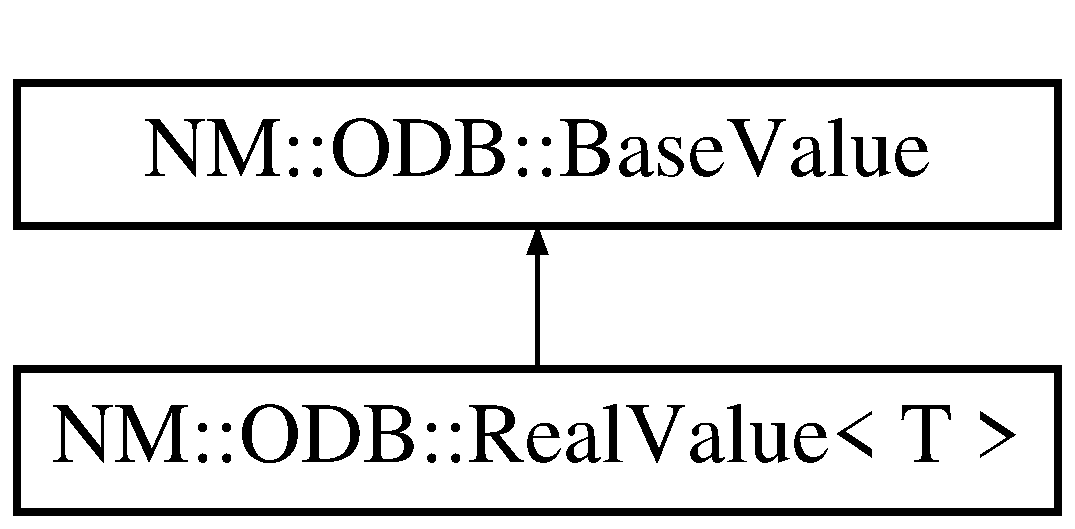
\includegraphics[height=2.000000cm]{class_n_m_1_1_o_d_b_1_1_base_value}
\end{center}
\end{figure}
\subsection*{Public Member Functions}
\begin{DoxyCompactItemize}
\item 
virtual \hyperlink{class_n_m_1_1_o_d_b_1_1_base_value}{Base\+Value} $\ast$ \hyperlink{class_n_m_1_1_o_d_b_1_1_base_value_a6e8d5f0d19f1be681fcf582e98cfdfa9}{Clone} () const  =0
\item 
virtual void \hyperlink{class_n_m_1_1_o_d_b_1_1_base_value_a343cd72d2116513509db379f6faab465}{Set} (\hyperlink{class_n_m_1_1_o_d_b_1_1_value}{Value} const \&v)=0
\item 
virtual \hyperlink{class_n_m_1_1_o_d_b_1_1_base_value_a85d4298ce766499ea78951361d89f301}{$\sim$\+Base\+Value} ()
\item 
virtual bool \hyperlink{class_n_m_1_1_o_d_b_1_1_base_value_a821b57552a15fd85e67f6d3949f19d4d}{operator==} (\hyperlink{class_n_m_1_1_o_d_b_1_1_base_value}{Base\+Value} const \&rhs)=0
\item 
virtual bool \hyperlink{class_n_m_1_1_o_d_b_1_1_base_value_ad6c041908183a43952a17dda329c372a}{operator$<$} (\hyperlink{class_n_m_1_1_o_d_b_1_1_base_value}{Base\+Value} const \&rhs)=0
\item 
virtual bool \hyperlink{class_n_m_1_1_o_d_b_1_1_base_value_aa36d79ee7fd479c798ea6adfabca0b06}{operator$>$} (\hyperlink{class_n_m_1_1_o_d_b_1_1_base_value}{Base\+Value} const \&rhs)=0
\item 
virtual \+::std\+::wstring \hyperlink{class_n_m_1_1_o_d_b_1_1_base_value_a1081e74053801b5c525c169e15f63fd3}{Get\+String\+Value} ()=0
\end{DoxyCompactItemize}
\subsection*{Protected Member Functions}
\begin{DoxyCompactItemize}
\item 
\hyperlink{class_n_m_1_1_o_d_b_1_1_base_value_ae8a04461840cfc4960e4157d962a7f26}{Base\+Value} ()
\end{DoxyCompactItemize}


\subsection{Detailed Description}
Class \hyperlink{class_n_m_1_1_o_d_b_1_1_base_value}{Base\+Value}

abstract baseclass for class \hyperlink{class_n_m_1_1_o_d_b_1_1_real_value}{Real\+Value} 

\subsection{Constructor \& Destructor Documentation}
\hypertarget{class_n_m_1_1_o_d_b_1_1_base_value_a85d4298ce766499ea78951361d89f301}{}\index{N\+M\+::\+O\+D\+B\+::\+Base\+Value@{N\+M\+::\+O\+D\+B\+::\+Base\+Value}!````~Base\+Value@{$\sim$\+Base\+Value}}
\index{````~Base\+Value@{$\sim$\+Base\+Value}!N\+M\+::\+O\+D\+B\+::\+Base\+Value@{N\+M\+::\+O\+D\+B\+::\+Base\+Value}}
\subsubsection[{$\sim$\+Base\+Value()}]{\setlength{\rightskip}{0pt plus 5cm}virtual N\+M\+::\+O\+D\+B\+::\+Base\+Value\+::$\sim$\+Base\+Value (
\begin{DoxyParamCaption}
{}
\end{DoxyParamCaption}
)\hspace{0.3cm}{\ttfamily [inline]}, {\ttfamily [virtual]}}\label{class_n_m_1_1_o_d_b_1_1_base_value_a85d4298ce766499ea78951361d89f301}
\hypertarget{class_n_m_1_1_o_d_b_1_1_base_value_ae8a04461840cfc4960e4157d962a7f26}{}\index{N\+M\+::\+O\+D\+B\+::\+Base\+Value@{N\+M\+::\+O\+D\+B\+::\+Base\+Value}!Base\+Value@{Base\+Value}}
\index{Base\+Value@{Base\+Value}!N\+M\+::\+O\+D\+B\+::\+Base\+Value@{N\+M\+::\+O\+D\+B\+::\+Base\+Value}}
\subsubsection[{Base\+Value()}]{\setlength{\rightskip}{0pt plus 5cm}N\+M\+::\+O\+D\+B\+::\+Base\+Value\+::\+Base\+Value (
\begin{DoxyParamCaption}
{}
\end{DoxyParamCaption}
)\hspace{0.3cm}{\ttfamily [inline]}, {\ttfamily [protected]}}\label{class_n_m_1_1_o_d_b_1_1_base_value_ae8a04461840cfc4960e4157d962a7f26}


\subsection{Member Function Documentation}
\hypertarget{class_n_m_1_1_o_d_b_1_1_base_value_a6e8d5f0d19f1be681fcf582e98cfdfa9}{}\index{N\+M\+::\+O\+D\+B\+::\+Base\+Value@{N\+M\+::\+O\+D\+B\+::\+Base\+Value}!Clone@{Clone}}
\index{Clone@{Clone}!N\+M\+::\+O\+D\+B\+::\+Base\+Value@{N\+M\+::\+O\+D\+B\+::\+Base\+Value}}
\subsubsection[{Clone() const  =0}]{\setlength{\rightskip}{0pt plus 5cm}virtual {\bf Base\+Value}$\ast$ N\+M\+::\+O\+D\+B\+::\+Base\+Value\+::\+Clone (
\begin{DoxyParamCaption}
{}
\end{DoxyParamCaption}
) const\hspace{0.3cm}{\ttfamily [pure virtual]}}\label{class_n_m_1_1_o_d_b_1_1_base_value_a6e8d5f0d19f1be681fcf582e98cfdfa9}


Implemented in \hyperlink{class_n_m_1_1_o_d_b_1_1_real_value_aef8e2c45cf4001f5115d24f8beb1f4df}{N\+M\+::\+O\+D\+B\+::\+Real\+Value$<$ T $>$}.

\hypertarget{class_n_m_1_1_o_d_b_1_1_base_value_a1081e74053801b5c525c169e15f63fd3}{}\index{N\+M\+::\+O\+D\+B\+::\+Base\+Value@{N\+M\+::\+O\+D\+B\+::\+Base\+Value}!Get\+String\+Value@{Get\+String\+Value}}
\index{Get\+String\+Value@{Get\+String\+Value}!N\+M\+::\+O\+D\+B\+::\+Base\+Value@{N\+M\+::\+O\+D\+B\+::\+Base\+Value}}
\subsubsection[{Get\+String\+Value()=0}]{\setlength{\rightskip}{0pt plus 5cm}virtual \+::std\+::wstring N\+M\+::\+O\+D\+B\+::\+Base\+Value\+::\+Get\+String\+Value (
\begin{DoxyParamCaption}
{}
\end{DoxyParamCaption}
)\hspace{0.3cm}{\ttfamily [pure virtual]}}\label{class_n_m_1_1_o_d_b_1_1_base_value_a1081e74053801b5c525c169e15f63fd3}


Implemented in \hyperlink{class_n_m_1_1_o_d_b_1_1_real_value_ac34574ad4f573ea467b5469403379f14}{N\+M\+::\+O\+D\+B\+::\+Real\+Value$<$ T $>$}.

\hypertarget{class_n_m_1_1_o_d_b_1_1_base_value_ad6c041908183a43952a17dda329c372a}{}\index{N\+M\+::\+O\+D\+B\+::\+Base\+Value@{N\+M\+::\+O\+D\+B\+::\+Base\+Value}!operator$<$@{operator$<$}}
\index{operator$<$@{operator$<$}!N\+M\+::\+O\+D\+B\+::\+Base\+Value@{N\+M\+::\+O\+D\+B\+::\+Base\+Value}}
\subsubsection[{operator$<$(\+Base\+Value const \&rhs)=0}]{\setlength{\rightskip}{0pt plus 5cm}virtual bool N\+M\+::\+O\+D\+B\+::\+Base\+Value\+::operator$<$ (
\begin{DoxyParamCaption}
\item[{{\bf Base\+Value} const \&}]{rhs}
\end{DoxyParamCaption}
)\hspace{0.3cm}{\ttfamily [pure virtual]}}\label{class_n_m_1_1_o_d_b_1_1_base_value_ad6c041908183a43952a17dda329c372a}


Implemented in \hyperlink{class_n_m_1_1_o_d_b_1_1_real_value_ad517ae8cfd80888a798c17ecee7435fe}{N\+M\+::\+O\+D\+B\+::\+Real\+Value$<$ T $>$}.

\hypertarget{class_n_m_1_1_o_d_b_1_1_base_value_a821b57552a15fd85e67f6d3949f19d4d}{}\index{N\+M\+::\+O\+D\+B\+::\+Base\+Value@{N\+M\+::\+O\+D\+B\+::\+Base\+Value}!operator==@{operator==}}
\index{operator==@{operator==}!N\+M\+::\+O\+D\+B\+::\+Base\+Value@{N\+M\+::\+O\+D\+B\+::\+Base\+Value}}
\subsubsection[{operator==(\+Base\+Value const \&rhs)=0}]{\setlength{\rightskip}{0pt plus 5cm}virtual bool N\+M\+::\+O\+D\+B\+::\+Base\+Value\+::operator== (
\begin{DoxyParamCaption}
\item[{{\bf Base\+Value} const \&}]{rhs}
\end{DoxyParamCaption}
)\hspace{0.3cm}{\ttfamily [pure virtual]}}\label{class_n_m_1_1_o_d_b_1_1_base_value_a821b57552a15fd85e67f6d3949f19d4d}


Implemented in \hyperlink{class_n_m_1_1_o_d_b_1_1_real_value_a296f8da033d8e15c56d666b4df7fe93f}{N\+M\+::\+O\+D\+B\+::\+Real\+Value$<$ T $>$}.

\hypertarget{class_n_m_1_1_o_d_b_1_1_base_value_aa36d79ee7fd479c798ea6adfabca0b06}{}\index{N\+M\+::\+O\+D\+B\+::\+Base\+Value@{N\+M\+::\+O\+D\+B\+::\+Base\+Value}!operator$>$@{operator$>$}}
\index{operator$>$@{operator$>$}!N\+M\+::\+O\+D\+B\+::\+Base\+Value@{N\+M\+::\+O\+D\+B\+::\+Base\+Value}}
\subsubsection[{operator$>$(\+Base\+Value const \&rhs)=0}]{\setlength{\rightskip}{0pt plus 5cm}virtual bool N\+M\+::\+O\+D\+B\+::\+Base\+Value\+::operator$>$ (
\begin{DoxyParamCaption}
\item[{{\bf Base\+Value} const \&}]{rhs}
\end{DoxyParamCaption}
)\hspace{0.3cm}{\ttfamily [pure virtual]}}\label{class_n_m_1_1_o_d_b_1_1_base_value_aa36d79ee7fd479c798ea6adfabca0b06}


Implemented in \hyperlink{class_n_m_1_1_o_d_b_1_1_real_value_a4c7dfb8876b4963fc61104fc19de7b28}{N\+M\+::\+O\+D\+B\+::\+Real\+Value$<$ T $>$}.

\hypertarget{class_n_m_1_1_o_d_b_1_1_base_value_a343cd72d2116513509db379f6faab465}{}\index{N\+M\+::\+O\+D\+B\+::\+Base\+Value@{N\+M\+::\+O\+D\+B\+::\+Base\+Value}!Set@{Set}}
\index{Set@{Set}!N\+M\+::\+O\+D\+B\+::\+Base\+Value@{N\+M\+::\+O\+D\+B\+::\+Base\+Value}}
\subsubsection[{Set(\+Value const \&v)=0}]{\setlength{\rightskip}{0pt plus 5cm}virtual void N\+M\+::\+O\+D\+B\+::\+Base\+Value\+::\+Set (
\begin{DoxyParamCaption}
\item[{{\bf Value} const \&}]{v}
\end{DoxyParamCaption}
)\hspace{0.3cm}{\ttfamily [pure virtual]}}\label{class_n_m_1_1_o_d_b_1_1_base_value_a343cd72d2116513509db379f6faab465}


Implemented in \hyperlink{class_n_m_1_1_o_d_b_1_1_real_value_a51fcdc7f0511e26b923ccfc47e20cb08}{N\+M\+::\+O\+D\+B\+::\+Real\+Value$<$ T $>$}.



The documentation for this class was generated from the following file\+:\begin{DoxyCompactItemize}
\item 
C\+:/\+Users/\+Simon/\+Documents/\+Personal/\+Source Code/\+Projects/\+Network\+Modeller/\+Object\+Database/\+Database\+Core\+Elements/\hyperlink{_base_value_8h}{Base\+Value.\+h}\end{DoxyCompactItemize}

\hypertarget{class_n_m_1_1_o_d_b_1_1_c_adjacency_matrix}{}\section{N\+M\+:\+:O\+D\+B\+:\+:C\+Adjacency\+Matrix Class Reference}
\label{class_n_m_1_1_o_d_b_1_1_c_adjacency_matrix}\index{N\+M\+::\+O\+D\+B\+::\+C\+Adjacency\+Matrix@{N\+M\+::\+O\+D\+B\+::\+C\+Adjacency\+Matrix}}


{\ttfamily \#include $<$Adjacency\+Matrix.\+h$>$}

\subsection*{Public Types}
\begin{DoxyCompactItemize}
\item 
enum \hyperlink{class_n_m_1_1_o_d_b_1_1_c_adjacency_matrix_aa4f68c561981e4e158dec4a4a9a97093}{E\+D\+G\+E\+T\+Y\+P\+E} \{ \hyperlink{class_n_m_1_1_o_d_b_1_1_c_adjacency_matrix_aa4f68c561981e4e158dec4a4a9a97093a1817cdb4e014f88e7c6794db0504e9ad}{E\+D\+G\+E\+\_\+\+D\+I\+R\+E\+C\+T\+E\+D}, 
\hyperlink{class_n_m_1_1_o_d_b_1_1_c_adjacency_matrix_aa4f68c561981e4e158dec4a4a9a97093a538d2110c4fc4fac7461bc240c86a89e}{E\+D\+G\+E\+\_\+\+U\+N\+D\+I\+R\+E\+C\+T\+E\+D}
 \}
\item 
typedef \+::std\+::vector$<$ \hyperlink{namespace_n_m_1_1_o_d_b_a262b64fab56baaa96e18bac4ada88265}{O\+B\+J\+E\+C\+T\+U\+I\+D} $>$ \hyperlink{class_n_m_1_1_o_d_b_1_1_c_adjacency_matrix_ab898e602bacf35a9600621408c1fde25}{edgelist}
\item 
typedef \+::std\+::vector$<$ \hyperlink{namespace_n_m_1_1_o_d_b_a262b64fab56baaa96e18bac4ada88265}{O\+B\+J\+E\+C\+T\+U\+I\+D} $>$ \hyperlink{class_n_m_1_1_o_d_b_1_1_c_adjacency_matrix_a483ee6ddd603d9ec66d5f21d0f11ff03}{vertexlist}
\end{DoxyCompactItemize}
\subsection*{Public Member Functions}
\begin{DoxyCompactItemize}
\item 
\hyperlink{class_n_m_1_1_o_d_b_1_1_c_adjacency_matrix_a0e8396d3b62701ef050f7b43819dc217}{C\+Adjacency\+Matrix} (void)
\item 
\hyperlink{class_n_m_1_1_o_d_b_1_1_c_adjacency_matrix_a526eb801477d33094e800614b1e4b4a3}{$\sim$\+C\+Adjacency\+Matrix} (void)
\item 
void \hyperlink{class_n_m_1_1_o_d_b_1_1_c_adjacency_matrix_aed4e1441f1acb61060b5076a766154fd}{Create\+Vertex} (\hyperlink{namespace_n_m_1_1_o_d_b_a262b64fab56baaa96e18bac4ada88265}{O\+B\+J\+E\+C\+T\+U\+I\+D} vertex\+I\+D)
\item 
void \hyperlink{class_n_m_1_1_o_d_b_1_1_c_adjacency_matrix_ada545d95afc704db45d8de771ce90f46}{Create\+Edge} (\hyperlink{namespace_n_m_1_1_o_d_b_a262b64fab56baaa96e18bac4ada88265}{O\+B\+J\+E\+C\+T\+U\+I\+D} Vertex\+Src\+I\+D, \hyperlink{namespace_n_m_1_1_o_d_b_a262b64fab56baaa96e18bac4ada88265}{O\+B\+J\+E\+C\+T\+U\+I\+D} Vertex\+Dst\+I\+D, \hyperlink{namespace_n_m_1_1_o_d_b_a262b64fab56baaa96e18bac4ada88265}{O\+B\+J\+E\+C\+T\+U\+I\+D} eid, enum \hyperlink{class_n_m_1_1_o_d_b_1_1_c_adjacency_matrix_aa4f68c561981e4e158dec4a4a9a97093}{E\+D\+G\+E\+T\+Y\+P\+E} edgetype)
\item 
void \hyperlink{class_n_m_1_1_o_d_b_1_1_c_adjacency_matrix_a3c49a3adc6a27dfbc46b6f84cb9c48a5}{Delete\+Vertex} (\hyperlink{namespace_n_m_1_1_o_d_b_a262b64fab56baaa96e18bac4ada88265}{O\+B\+J\+E\+C\+T\+U\+I\+D} Vertex\+I\+D)
\item 
void \hyperlink{class_n_m_1_1_o_d_b_1_1_c_adjacency_matrix_a41bb80d3cc1f376e496b031f1ed7762d}{Delete\+Edge} (\hyperlink{namespace_n_m_1_1_o_d_b_a262b64fab56baaa96e18bac4ada88265}{O\+B\+J\+E\+C\+T\+U\+I\+D} Vertex\+Src\+I\+D, \hyperlink{namespace_n_m_1_1_o_d_b_a262b64fab56baaa96e18bac4ada88265}{O\+B\+J\+E\+C\+T\+U\+I\+D} Vertex\+Dst\+I\+D, \hyperlink{namespace_n_m_1_1_o_d_b_a262b64fab56baaa96e18bac4ada88265}{O\+B\+J\+E\+C\+T\+U\+I\+D} eid, enum \hyperlink{class_n_m_1_1_o_d_b_1_1_c_adjacency_matrix_aa4f68c561981e4e158dec4a4a9a97093}{E\+D\+G\+E\+T\+Y\+P\+E} edgetype)
\item 
void \hyperlink{class_n_m_1_1_o_d_b_1_1_c_adjacency_matrix_aef66ef8cc6d5ad26172960bf03412e5c}{Delete\+All\+Edges} (\hyperlink{namespace_n_m_1_1_o_d_b_a262b64fab56baaa96e18bac4ada88265}{O\+B\+J\+E\+C\+T\+U\+I\+D} Vertex\+Src\+I\+D, \hyperlink{namespace_n_m_1_1_o_d_b_a262b64fab56baaa96e18bac4ada88265}{O\+B\+J\+E\+C\+T\+U\+I\+D} Vertex\+Dst\+I\+D, enum \hyperlink{class_n_m_1_1_o_d_b_1_1_c_adjacency_matrix_aa4f68c561981e4e158dec4a4a9a97093}{E\+D\+G\+E\+T\+Y\+P\+E} edgetype)
\item 
void \hyperlink{class_n_m_1_1_o_d_b_1_1_c_adjacency_matrix_ac9d09accdbb67dcf8762da978bd4f828}{Clear} ()
\item 
size\+\_\+t \hyperlink{class_n_m_1_1_o_d_b_1_1_c_adjacency_matrix_a13acffafe60d081aa33cd572c2437cf2}{Get\+Vertex\+Connected\+Verticies} (\hyperlink{namespace_n_m_1_1_o_d_b_a262b64fab56baaa96e18bac4ada88265}{O\+B\+J\+E\+C\+T\+U\+I\+D} Vertex\+I\+D,\+::std\+::vector$<$ \hyperlink{namespace_n_m_1_1_o_d_b_a262b64fab56baaa96e18bac4ada88265}{O\+B\+J\+E\+C\+T\+U\+I\+D} $>$ \&\hyperlink{class_n_m_1_1_o_d_b_1_1_c_adjacency_matrix_a483ee6ddd603d9ec66d5f21d0f11ff03}{vertexlist})
\item 
size\+\_\+t \hyperlink{class_n_m_1_1_o_d_b_1_1_c_adjacency_matrix_a83d73a80157035ae5dff7374745b581a}{Get\+Vertex\+Connected\+Edge\+Count} (\hyperlink{namespace_n_m_1_1_o_d_b_a262b64fab56baaa96e18bac4ada88265}{O\+B\+J\+E\+C\+T\+U\+I\+D} src\+Vertex\+I\+D, \hyperlink{namespace_n_m_1_1_o_d_b_a262b64fab56baaa96e18bac4ada88265}{O\+B\+J\+E\+C\+T\+U\+I\+D} dst\+Vertex\+I\+D)
\item 
void \hyperlink{class_n_m_1_1_o_d_b_1_1_c_adjacency_matrix_ad183137a9098789b779d698bf45cae24}{Get\+Vertex\+Connected\+Edges} (\hyperlink{namespace_n_m_1_1_o_d_b_a262b64fab56baaa96e18bac4ada88265}{O\+B\+J\+E\+C\+T\+U\+I\+D} src\+Vertex\+I\+D, \hyperlink{namespace_n_m_1_1_o_d_b_a262b64fab56baaa96e18bac4ada88265}{O\+B\+J\+E\+C\+T\+U\+I\+D} dst\+Vertex\+I\+D,\+::std\+::vector$<$ \hyperlink{namespace_n_m_1_1_o_d_b_a262b64fab56baaa96e18bac4ada88265}{O\+B\+J\+E\+C\+T\+U\+I\+D} $>$ \&\hyperlink{class_n_m_1_1_o_d_b_1_1_c_adjacency_matrix_ab898e602bacf35a9600621408c1fde25}{edgelist})
\item 
void \hyperlink{class_n_m_1_1_o_d_b_1_1_c_adjacency_matrix_a72db29148daa6a3b4910ac6387e1f089}{Get\+Vertex\+Edges} (\hyperlink{namespace_n_m_1_1_o_d_b_a262b64fab56baaa96e18bac4ada88265}{O\+B\+J\+E\+C\+T\+U\+I\+D} Vertex\+I\+D,\+::std\+::vector$<$ \hyperlink{namespace_n_m_1_1_o_d_b_a262b64fab56baaa96e18bac4ada88265}{O\+B\+J\+E\+C\+T\+U\+I\+D} $>$ \&\hyperlink{class_n_m_1_1_o_d_b_1_1_c_adjacency_matrix_ab898e602bacf35a9600621408c1fde25}{edgelist})
\item 
size\+\_\+t \hyperlink{class_n_m_1_1_o_d_b_1_1_c_adjacency_matrix_a43b0a584fc5d0a41e00dd5f035997bb1}{Get\+Vertex\+Degree} (\hyperlink{namespace_n_m_1_1_o_d_b_a262b64fab56baaa96e18bac4ada88265}{O\+B\+J\+E\+C\+T\+U\+I\+D} Vertex\+I\+D)
\item 
void \hyperlink{class_n_m_1_1_o_d_b_1_1_c_adjacency_matrix_a7ae4ee21d0762cce032c053f3c55aaaf}{Get\+Matrix\+Size} (size\+\_\+t \&rows, size\+\_\+t \&cols)
\item 
void \hyperlink{class_n_m_1_1_o_d_b_1_1_c_adjacency_matrix_a76db9fc9c3204f188e2de2329367e626}{Output\+Matrix\+To\+Console} ()
\end{DoxyCompactItemize}


\subsection{Member Typedef Documentation}
\hypertarget{class_n_m_1_1_o_d_b_1_1_c_adjacency_matrix_ab898e602bacf35a9600621408c1fde25}{}\index{N\+M\+::\+O\+D\+B\+::\+C\+Adjacency\+Matrix@{N\+M\+::\+O\+D\+B\+::\+C\+Adjacency\+Matrix}!edgelist@{edgelist}}
\index{edgelist@{edgelist}!N\+M\+::\+O\+D\+B\+::\+C\+Adjacency\+Matrix@{N\+M\+::\+O\+D\+B\+::\+C\+Adjacency\+Matrix}}
\subsubsection[{edgelist}]{\setlength{\rightskip}{0pt plus 5cm}typedef \+::std\+::vector$<${\bf O\+B\+J\+E\+C\+T\+U\+I\+D}$>$ {\bf N\+M\+::\+O\+D\+B\+::\+C\+Adjacency\+Matrix\+::edgelist}}\label{class_n_m_1_1_o_d_b_1_1_c_adjacency_matrix_ab898e602bacf35a9600621408c1fde25}
\hypertarget{class_n_m_1_1_o_d_b_1_1_c_adjacency_matrix_a483ee6ddd603d9ec66d5f21d0f11ff03}{}\index{N\+M\+::\+O\+D\+B\+::\+C\+Adjacency\+Matrix@{N\+M\+::\+O\+D\+B\+::\+C\+Adjacency\+Matrix}!vertexlist@{vertexlist}}
\index{vertexlist@{vertexlist}!N\+M\+::\+O\+D\+B\+::\+C\+Adjacency\+Matrix@{N\+M\+::\+O\+D\+B\+::\+C\+Adjacency\+Matrix}}
\subsubsection[{vertexlist}]{\setlength{\rightskip}{0pt plus 5cm}typedef \+::std\+::vector$<${\bf O\+B\+J\+E\+C\+T\+U\+I\+D}$>$ {\bf N\+M\+::\+O\+D\+B\+::\+C\+Adjacency\+Matrix\+::vertexlist}}\label{class_n_m_1_1_o_d_b_1_1_c_adjacency_matrix_a483ee6ddd603d9ec66d5f21d0f11ff03}


\subsection{Member Enumeration Documentation}
\hypertarget{class_n_m_1_1_o_d_b_1_1_c_adjacency_matrix_aa4f68c561981e4e158dec4a4a9a97093}{}\index{N\+M\+::\+O\+D\+B\+::\+C\+Adjacency\+Matrix@{N\+M\+::\+O\+D\+B\+::\+C\+Adjacency\+Matrix}!E\+D\+G\+E\+T\+Y\+P\+E@{E\+D\+G\+E\+T\+Y\+P\+E}}
\index{E\+D\+G\+E\+T\+Y\+P\+E@{E\+D\+G\+E\+T\+Y\+P\+E}!N\+M\+::\+O\+D\+B\+::\+C\+Adjacency\+Matrix@{N\+M\+::\+O\+D\+B\+::\+C\+Adjacency\+Matrix}}
\subsubsection[{E\+D\+G\+E\+T\+Y\+P\+E}]{\setlength{\rightskip}{0pt plus 5cm}enum {\bf N\+M\+::\+O\+D\+B\+::\+C\+Adjacency\+Matrix\+::\+E\+D\+G\+E\+T\+Y\+P\+E}}\label{class_n_m_1_1_o_d_b_1_1_c_adjacency_matrix_aa4f68c561981e4e158dec4a4a9a97093}
\begin{Desc}
\item[Enumerator]\par
\begin{description}
\index{E\+D\+G\+E\+\_\+\+D\+I\+R\+E\+C\+T\+E\+D@{E\+D\+G\+E\+\_\+\+D\+I\+R\+E\+C\+T\+E\+D}!N\+M\+::\+O\+D\+B\+::\+C\+Adjacency\+Matrix@{N\+M\+::\+O\+D\+B\+::\+C\+Adjacency\+Matrix}}\index{N\+M\+::\+O\+D\+B\+::\+C\+Adjacency\+Matrix@{N\+M\+::\+O\+D\+B\+::\+C\+Adjacency\+Matrix}!E\+D\+G\+E\+\_\+\+D\+I\+R\+E\+C\+T\+E\+D@{E\+D\+G\+E\+\_\+\+D\+I\+R\+E\+C\+T\+E\+D}}\item[{\em 
\hypertarget{class_n_m_1_1_o_d_b_1_1_c_adjacency_matrix_aa4f68c561981e4e158dec4a4a9a97093a1817cdb4e014f88e7c6794db0504e9ad}{}E\+D\+G\+E\+\_\+\+D\+I\+R\+E\+C\+T\+E\+D\label{class_n_m_1_1_o_d_b_1_1_c_adjacency_matrix_aa4f68c561981e4e158dec4a4a9a97093a1817cdb4e014f88e7c6794db0504e9ad}
}]\index{E\+D\+G\+E\+\_\+\+U\+N\+D\+I\+R\+E\+C\+T\+E\+D@{E\+D\+G\+E\+\_\+\+U\+N\+D\+I\+R\+E\+C\+T\+E\+D}!N\+M\+::\+O\+D\+B\+::\+C\+Adjacency\+Matrix@{N\+M\+::\+O\+D\+B\+::\+C\+Adjacency\+Matrix}}\index{N\+M\+::\+O\+D\+B\+::\+C\+Adjacency\+Matrix@{N\+M\+::\+O\+D\+B\+::\+C\+Adjacency\+Matrix}!E\+D\+G\+E\+\_\+\+U\+N\+D\+I\+R\+E\+C\+T\+E\+D@{E\+D\+G\+E\+\_\+\+U\+N\+D\+I\+R\+E\+C\+T\+E\+D}}\item[{\em 
\hypertarget{class_n_m_1_1_o_d_b_1_1_c_adjacency_matrix_aa4f68c561981e4e158dec4a4a9a97093a538d2110c4fc4fac7461bc240c86a89e}{}E\+D\+G\+E\+\_\+\+U\+N\+D\+I\+R\+E\+C\+T\+E\+D\label{class_n_m_1_1_o_d_b_1_1_c_adjacency_matrix_aa4f68c561981e4e158dec4a4a9a97093a538d2110c4fc4fac7461bc240c86a89e}
}]\end{description}
\end{Desc}


\subsection{Constructor \& Destructor Documentation}
\hypertarget{class_n_m_1_1_o_d_b_1_1_c_adjacency_matrix_a0e8396d3b62701ef050f7b43819dc217}{}\index{N\+M\+::\+O\+D\+B\+::\+C\+Adjacency\+Matrix@{N\+M\+::\+O\+D\+B\+::\+C\+Adjacency\+Matrix}!C\+Adjacency\+Matrix@{C\+Adjacency\+Matrix}}
\index{C\+Adjacency\+Matrix@{C\+Adjacency\+Matrix}!N\+M\+::\+O\+D\+B\+::\+C\+Adjacency\+Matrix@{N\+M\+::\+O\+D\+B\+::\+C\+Adjacency\+Matrix}}
\subsubsection[{C\+Adjacency\+Matrix(void)}]{\setlength{\rightskip}{0pt plus 5cm}N\+M\+::\+O\+D\+B\+::\+C\+Adjacency\+Matrix\+::\+C\+Adjacency\+Matrix (
\begin{DoxyParamCaption}
\item[{void}]{}
\end{DoxyParamCaption}
)}\label{class_n_m_1_1_o_d_b_1_1_c_adjacency_matrix_a0e8396d3b62701ef050f7b43819dc217}
\hypertarget{class_n_m_1_1_o_d_b_1_1_c_adjacency_matrix_a526eb801477d33094e800614b1e4b4a3}{}\index{N\+M\+::\+O\+D\+B\+::\+C\+Adjacency\+Matrix@{N\+M\+::\+O\+D\+B\+::\+C\+Adjacency\+Matrix}!````~C\+Adjacency\+Matrix@{$\sim$\+C\+Adjacency\+Matrix}}
\index{````~C\+Adjacency\+Matrix@{$\sim$\+C\+Adjacency\+Matrix}!N\+M\+::\+O\+D\+B\+::\+C\+Adjacency\+Matrix@{N\+M\+::\+O\+D\+B\+::\+C\+Adjacency\+Matrix}}
\subsubsection[{$\sim$\+C\+Adjacency\+Matrix(void)}]{\setlength{\rightskip}{0pt plus 5cm}N\+M\+::\+O\+D\+B\+::\+C\+Adjacency\+Matrix\+::$\sim$\+C\+Adjacency\+Matrix (
\begin{DoxyParamCaption}
\item[{void}]{}
\end{DoxyParamCaption}
)}\label{class_n_m_1_1_o_d_b_1_1_c_adjacency_matrix_a526eb801477d33094e800614b1e4b4a3}


\subsection{Member Function Documentation}
\hypertarget{class_n_m_1_1_o_d_b_1_1_c_adjacency_matrix_ac9d09accdbb67dcf8762da978bd4f828}{}\index{N\+M\+::\+O\+D\+B\+::\+C\+Adjacency\+Matrix@{N\+M\+::\+O\+D\+B\+::\+C\+Adjacency\+Matrix}!Clear@{Clear}}
\index{Clear@{Clear}!N\+M\+::\+O\+D\+B\+::\+C\+Adjacency\+Matrix@{N\+M\+::\+O\+D\+B\+::\+C\+Adjacency\+Matrix}}
\subsubsection[{Clear()}]{\setlength{\rightskip}{0pt plus 5cm}void N\+M\+::\+O\+D\+B\+::\+C\+Adjacency\+Matrix\+::\+Clear (
\begin{DoxyParamCaption}
{}
\end{DoxyParamCaption}
)}\label{class_n_m_1_1_o_d_b_1_1_c_adjacency_matrix_ac9d09accdbb67dcf8762da978bd4f828}
\hypertarget{class_n_m_1_1_o_d_b_1_1_c_adjacency_matrix_ada545d95afc704db45d8de771ce90f46}{}\index{N\+M\+::\+O\+D\+B\+::\+C\+Adjacency\+Matrix@{N\+M\+::\+O\+D\+B\+::\+C\+Adjacency\+Matrix}!Create\+Edge@{Create\+Edge}}
\index{Create\+Edge@{Create\+Edge}!N\+M\+::\+O\+D\+B\+::\+C\+Adjacency\+Matrix@{N\+M\+::\+O\+D\+B\+::\+C\+Adjacency\+Matrix}}
\subsubsection[{Create\+Edge(\+O\+B\+J\+E\+C\+T\+U\+I\+D Vertex\+Src\+I\+D, O\+B\+J\+E\+C\+T\+U\+I\+D Vertex\+Dst\+I\+D, O\+B\+J\+E\+C\+T\+U\+I\+D eid, enum E\+D\+G\+E\+T\+Y\+P\+E edgetype)}]{\setlength{\rightskip}{0pt plus 5cm}void N\+M\+::\+O\+D\+B\+::\+C\+Adjacency\+Matrix\+::\+Create\+Edge (
\begin{DoxyParamCaption}
\item[{{\bf O\+B\+J\+E\+C\+T\+U\+I\+D}}]{Vertex\+Src\+I\+D, }
\item[{{\bf O\+B\+J\+E\+C\+T\+U\+I\+D}}]{Vertex\+Dst\+I\+D, }
\item[{{\bf O\+B\+J\+E\+C\+T\+U\+I\+D}}]{eid, }
\item[{enum {\bf E\+D\+G\+E\+T\+Y\+P\+E}}]{edgetype}
\end{DoxyParamCaption}
)}\label{class_n_m_1_1_o_d_b_1_1_c_adjacency_matrix_ada545d95afc704db45d8de771ce90f46}
\hypertarget{class_n_m_1_1_o_d_b_1_1_c_adjacency_matrix_aed4e1441f1acb61060b5076a766154fd}{}\index{N\+M\+::\+O\+D\+B\+::\+C\+Adjacency\+Matrix@{N\+M\+::\+O\+D\+B\+::\+C\+Adjacency\+Matrix}!Create\+Vertex@{Create\+Vertex}}
\index{Create\+Vertex@{Create\+Vertex}!N\+M\+::\+O\+D\+B\+::\+C\+Adjacency\+Matrix@{N\+M\+::\+O\+D\+B\+::\+C\+Adjacency\+Matrix}}
\subsubsection[{Create\+Vertex(\+O\+B\+J\+E\+C\+T\+U\+I\+D vertex\+I\+D)}]{\setlength{\rightskip}{0pt plus 5cm}void N\+M\+::\+O\+D\+B\+::\+C\+Adjacency\+Matrix\+::\+Create\+Vertex (
\begin{DoxyParamCaption}
\item[{{\bf O\+B\+J\+E\+C\+T\+U\+I\+D}}]{vertex\+I\+D}
\end{DoxyParamCaption}
)}\label{class_n_m_1_1_o_d_b_1_1_c_adjacency_matrix_aed4e1441f1acb61060b5076a766154fd}
\hypertarget{class_n_m_1_1_o_d_b_1_1_c_adjacency_matrix_aef66ef8cc6d5ad26172960bf03412e5c}{}\index{N\+M\+::\+O\+D\+B\+::\+C\+Adjacency\+Matrix@{N\+M\+::\+O\+D\+B\+::\+C\+Adjacency\+Matrix}!Delete\+All\+Edges@{Delete\+All\+Edges}}
\index{Delete\+All\+Edges@{Delete\+All\+Edges}!N\+M\+::\+O\+D\+B\+::\+C\+Adjacency\+Matrix@{N\+M\+::\+O\+D\+B\+::\+C\+Adjacency\+Matrix}}
\subsubsection[{Delete\+All\+Edges(\+O\+B\+J\+E\+C\+T\+U\+I\+D Vertex\+Src\+I\+D, O\+B\+J\+E\+C\+T\+U\+I\+D Vertex\+Dst\+I\+D, enum E\+D\+G\+E\+T\+Y\+P\+E edgetype)}]{\setlength{\rightskip}{0pt plus 5cm}void N\+M\+::\+O\+D\+B\+::\+C\+Adjacency\+Matrix\+::\+Delete\+All\+Edges (
\begin{DoxyParamCaption}
\item[{{\bf O\+B\+J\+E\+C\+T\+U\+I\+D}}]{Vertex\+Src\+I\+D, }
\item[{{\bf O\+B\+J\+E\+C\+T\+U\+I\+D}}]{Vertex\+Dst\+I\+D, }
\item[{enum {\bf E\+D\+G\+E\+T\+Y\+P\+E}}]{edgetype}
\end{DoxyParamCaption}
)}\label{class_n_m_1_1_o_d_b_1_1_c_adjacency_matrix_aef66ef8cc6d5ad26172960bf03412e5c}
\hypertarget{class_n_m_1_1_o_d_b_1_1_c_adjacency_matrix_a41bb80d3cc1f376e496b031f1ed7762d}{}\index{N\+M\+::\+O\+D\+B\+::\+C\+Adjacency\+Matrix@{N\+M\+::\+O\+D\+B\+::\+C\+Adjacency\+Matrix}!Delete\+Edge@{Delete\+Edge}}
\index{Delete\+Edge@{Delete\+Edge}!N\+M\+::\+O\+D\+B\+::\+C\+Adjacency\+Matrix@{N\+M\+::\+O\+D\+B\+::\+C\+Adjacency\+Matrix}}
\subsubsection[{Delete\+Edge(\+O\+B\+J\+E\+C\+T\+U\+I\+D Vertex\+Src\+I\+D, O\+B\+J\+E\+C\+T\+U\+I\+D Vertex\+Dst\+I\+D, O\+B\+J\+E\+C\+T\+U\+I\+D eid, enum E\+D\+G\+E\+T\+Y\+P\+E edgetype)}]{\setlength{\rightskip}{0pt plus 5cm}void N\+M\+::\+O\+D\+B\+::\+C\+Adjacency\+Matrix\+::\+Delete\+Edge (
\begin{DoxyParamCaption}
\item[{{\bf O\+B\+J\+E\+C\+T\+U\+I\+D}}]{Vertex\+Src\+I\+D, }
\item[{{\bf O\+B\+J\+E\+C\+T\+U\+I\+D}}]{Vertex\+Dst\+I\+D, }
\item[{{\bf O\+B\+J\+E\+C\+T\+U\+I\+D}}]{eid, }
\item[{enum {\bf E\+D\+G\+E\+T\+Y\+P\+E}}]{edgetype}
\end{DoxyParamCaption}
)}\label{class_n_m_1_1_o_d_b_1_1_c_adjacency_matrix_a41bb80d3cc1f376e496b031f1ed7762d}
\hypertarget{class_n_m_1_1_o_d_b_1_1_c_adjacency_matrix_a3c49a3adc6a27dfbc46b6f84cb9c48a5}{}\index{N\+M\+::\+O\+D\+B\+::\+C\+Adjacency\+Matrix@{N\+M\+::\+O\+D\+B\+::\+C\+Adjacency\+Matrix}!Delete\+Vertex@{Delete\+Vertex}}
\index{Delete\+Vertex@{Delete\+Vertex}!N\+M\+::\+O\+D\+B\+::\+C\+Adjacency\+Matrix@{N\+M\+::\+O\+D\+B\+::\+C\+Adjacency\+Matrix}}
\subsubsection[{Delete\+Vertex(\+O\+B\+J\+E\+C\+T\+U\+I\+D Vertex\+I\+D)}]{\setlength{\rightskip}{0pt plus 5cm}void N\+M\+::\+O\+D\+B\+::\+C\+Adjacency\+Matrix\+::\+Delete\+Vertex (
\begin{DoxyParamCaption}
\item[{{\bf O\+B\+J\+E\+C\+T\+U\+I\+D}}]{Vertex\+I\+D}
\end{DoxyParamCaption}
)}\label{class_n_m_1_1_o_d_b_1_1_c_adjacency_matrix_a3c49a3adc6a27dfbc46b6f84cb9c48a5}
\hypertarget{class_n_m_1_1_o_d_b_1_1_c_adjacency_matrix_a7ae4ee21d0762cce032c053f3c55aaaf}{}\index{N\+M\+::\+O\+D\+B\+::\+C\+Adjacency\+Matrix@{N\+M\+::\+O\+D\+B\+::\+C\+Adjacency\+Matrix}!Get\+Matrix\+Size@{Get\+Matrix\+Size}}
\index{Get\+Matrix\+Size@{Get\+Matrix\+Size}!N\+M\+::\+O\+D\+B\+::\+C\+Adjacency\+Matrix@{N\+M\+::\+O\+D\+B\+::\+C\+Adjacency\+Matrix}}
\subsubsection[{Get\+Matrix\+Size(size\+\_\+t \&rows, size\+\_\+t \&cols)}]{\setlength{\rightskip}{0pt plus 5cm}void N\+M\+::\+O\+D\+B\+::\+C\+Adjacency\+Matrix\+::\+Get\+Matrix\+Size (
\begin{DoxyParamCaption}
\item[{size\+\_\+t \&}]{rows, }
\item[{size\+\_\+t \&}]{cols}
\end{DoxyParamCaption}
)}\label{class_n_m_1_1_o_d_b_1_1_c_adjacency_matrix_a7ae4ee21d0762cce032c053f3c55aaaf}
\hypertarget{class_n_m_1_1_o_d_b_1_1_c_adjacency_matrix_a83d73a80157035ae5dff7374745b581a}{}\index{N\+M\+::\+O\+D\+B\+::\+C\+Adjacency\+Matrix@{N\+M\+::\+O\+D\+B\+::\+C\+Adjacency\+Matrix}!Get\+Vertex\+Connected\+Edge\+Count@{Get\+Vertex\+Connected\+Edge\+Count}}
\index{Get\+Vertex\+Connected\+Edge\+Count@{Get\+Vertex\+Connected\+Edge\+Count}!N\+M\+::\+O\+D\+B\+::\+C\+Adjacency\+Matrix@{N\+M\+::\+O\+D\+B\+::\+C\+Adjacency\+Matrix}}
\subsubsection[{Get\+Vertex\+Connected\+Edge\+Count(\+O\+B\+J\+E\+C\+T\+U\+I\+D src\+Vertex\+I\+D, O\+B\+J\+E\+C\+T\+U\+I\+D dst\+Vertex\+I\+D)}]{\setlength{\rightskip}{0pt plus 5cm}size\+\_\+t N\+M\+::\+O\+D\+B\+::\+C\+Adjacency\+Matrix\+::\+Get\+Vertex\+Connected\+Edge\+Count (
\begin{DoxyParamCaption}
\item[{{\bf O\+B\+J\+E\+C\+T\+U\+I\+D}}]{src\+Vertex\+I\+D, }
\item[{{\bf O\+B\+J\+E\+C\+T\+U\+I\+D}}]{dst\+Vertex\+I\+D}
\end{DoxyParamCaption}
)}\label{class_n_m_1_1_o_d_b_1_1_c_adjacency_matrix_a83d73a80157035ae5dff7374745b581a}
\hypertarget{class_n_m_1_1_o_d_b_1_1_c_adjacency_matrix_ad183137a9098789b779d698bf45cae24}{}\index{N\+M\+::\+O\+D\+B\+::\+C\+Adjacency\+Matrix@{N\+M\+::\+O\+D\+B\+::\+C\+Adjacency\+Matrix}!Get\+Vertex\+Connected\+Edges@{Get\+Vertex\+Connected\+Edges}}
\index{Get\+Vertex\+Connected\+Edges@{Get\+Vertex\+Connected\+Edges}!N\+M\+::\+O\+D\+B\+::\+C\+Adjacency\+Matrix@{N\+M\+::\+O\+D\+B\+::\+C\+Adjacency\+Matrix}}
\subsubsection[{Get\+Vertex\+Connected\+Edges(\+O\+B\+J\+E\+C\+T\+U\+I\+D src\+Vertex\+I\+D, O\+B\+J\+E\+C\+T\+U\+I\+D dst\+Vertex\+I\+D,\+::std\+::vector$<$ O\+B\+J\+E\+C\+T\+U\+I\+D $>$ \&edgelist)}]{\setlength{\rightskip}{0pt plus 5cm}void N\+M\+::\+O\+D\+B\+::\+C\+Adjacency\+Matrix\+::\+Get\+Vertex\+Connected\+Edges (
\begin{DoxyParamCaption}
\item[{{\bf O\+B\+J\+E\+C\+T\+U\+I\+D}}]{src\+Vertex\+I\+D, }
\item[{{\bf O\+B\+J\+E\+C\+T\+U\+I\+D}}]{dst\+Vertex\+I\+D, }
\item[{\+::std\+::vector$<$ {\bf O\+B\+J\+E\+C\+T\+U\+I\+D} $>$ \&}]{edgelist}
\end{DoxyParamCaption}
)}\label{class_n_m_1_1_o_d_b_1_1_c_adjacency_matrix_ad183137a9098789b779d698bf45cae24}
\hypertarget{class_n_m_1_1_o_d_b_1_1_c_adjacency_matrix_a13acffafe60d081aa33cd572c2437cf2}{}\index{N\+M\+::\+O\+D\+B\+::\+C\+Adjacency\+Matrix@{N\+M\+::\+O\+D\+B\+::\+C\+Adjacency\+Matrix}!Get\+Vertex\+Connected\+Verticies@{Get\+Vertex\+Connected\+Verticies}}
\index{Get\+Vertex\+Connected\+Verticies@{Get\+Vertex\+Connected\+Verticies}!N\+M\+::\+O\+D\+B\+::\+C\+Adjacency\+Matrix@{N\+M\+::\+O\+D\+B\+::\+C\+Adjacency\+Matrix}}
\subsubsection[{Get\+Vertex\+Connected\+Verticies(\+O\+B\+J\+E\+C\+T\+U\+I\+D Vertex\+I\+D,\+::std\+::vector$<$ O\+B\+J\+E\+C\+T\+U\+I\+D $>$ \&vertexlist)}]{\setlength{\rightskip}{0pt plus 5cm}size\+\_\+t N\+M\+::\+O\+D\+B\+::\+C\+Adjacency\+Matrix\+::\+Get\+Vertex\+Connected\+Verticies (
\begin{DoxyParamCaption}
\item[{{\bf O\+B\+J\+E\+C\+T\+U\+I\+D}}]{Vertex\+I\+D, }
\item[{\+::std\+::vector$<$ {\bf O\+B\+J\+E\+C\+T\+U\+I\+D} $>$ \&}]{vertexlist}
\end{DoxyParamCaption}
)}\label{class_n_m_1_1_o_d_b_1_1_c_adjacency_matrix_a13acffafe60d081aa33cd572c2437cf2}
\hypertarget{class_n_m_1_1_o_d_b_1_1_c_adjacency_matrix_a43b0a584fc5d0a41e00dd5f035997bb1}{}\index{N\+M\+::\+O\+D\+B\+::\+C\+Adjacency\+Matrix@{N\+M\+::\+O\+D\+B\+::\+C\+Adjacency\+Matrix}!Get\+Vertex\+Degree@{Get\+Vertex\+Degree}}
\index{Get\+Vertex\+Degree@{Get\+Vertex\+Degree}!N\+M\+::\+O\+D\+B\+::\+C\+Adjacency\+Matrix@{N\+M\+::\+O\+D\+B\+::\+C\+Adjacency\+Matrix}}
\subsubsection[{Get\+Vertex\+Degree(\+O\+B\+J\+E\+C\+T\+U\+I\+D Vertex\+I\+D)}]{\setlength{\rightskip}{0pt plus 5cm}size\+\_\+t N\+M\+::\+O\+D\+B\+::\+C\+Adjacency\+Matrix\+::\+Get\+Vertex\+Degree (
\begin{DoxyParamCaption}
\item[{{\bf O\+B\+J\+E\+C\+T\+U\+I\+D}}]{Vertex\+I\+D}
\end{DoxyParamCaption}
)}\label{class_n_m_1_1_o_d_b_1_1_c_adjacency_matrix_a43b0a584fc5d0a41e00dd5f035997bb1}
\hypertarget{class_n_m_1_1_o_d_b_1_1_c_adjacency_matrix_a72db29148daa6a3b4910ac6387e1f089}{}\index{N\+M\+::\+O\+D\+B\+::\+C\+Adjacency\+Matrix@{N\+M\+::\+O\+D\+B\+::\+C\+Adjacency\+Matrix}!Get\+Vertex\+Edges@{Get\+Vertex\+Edges}}
\index{Get\+Vertex\+Edges@{Get\+Vertex\+Edges}!N\+M\+::\+O\+D\+B\+::\+C\+Adjacency\+Matrix@{N\+M\+::\+O\+D\+B\+::\+C\+Adjacency\+Matrix}}
\subsubsection[{Get\+Vertex\+Edges(\+O\+B\+J\+E\+C\+T\+U\+I\+D Vertex\+I\+D,\+::std\+::vector$<$ O\+B\+J\+E\+C\+T\+U\+I\+D $>$ \&edgelist)}]{\setlength{\rightskip}{0pt plus 5cm}void N\+M\+::\+O\+D\+B\+::\+C\+Adjacency\+Matrix\+::\+Get\+Vertex\+Edges (
\begin{DoxyParamCaption}
\item[{{\bf O\+B\+J\+E\+C\+T\+U\+I\+D}}]{Vertex\+I\+D, }
\item[{\+::std\+::vector$<$ {\bf O\+B\+J\+E\+C\+T\+U\+I\+D} $>$ \&}]{edgelist}
\end{DoxyParamCaption}
)}\label{class_n_m_1_1_o_d_b_1_1_c_adjacency_matrix_a72db29148daa6a3b4910ac6387e1f089}
\hypertarget{class_n_m_1_1_o_d_b_1_1_c_adjacency_matrix_a76db9fc9c3204f188e2de2329367e626}{}\index{N\+M\+::\+O\+D\+B\+::\+C\+Adjacency\+Matrix@{N\+M\+::\+O\+D\+B\+::\+C\+Adjacency\+Matrix}!Output\+Matrix\+To\+Console@{Output\+Matrix\+To\+Console}}
\index{Output\+Matrix\+To\+Console@{Output\+Matrix\+To\+Console}!N\+M\+::\+O\+D\+B\+::\+C\+Adjacency\+Matrix@{N\+M\+::\+O\+D\+B\+::\+C\+Adjacency\+Matrix}}
\subsubsection[{Output\+Matrix\+To\+Console()}]{\setlength{\rightskip}{0pt plus 5cm}void N\+M\+::\+O\+D\+B\+::\+C\+Adjacency\+Matrix\+::\+Output\+Matrix\+To\+Console (
\begin{DoxyParamCaption}
{}
\end{DoxyParamCaption}
)}\label{class_n_m_1_1_o_d_b_1_1_c_adjacency_matrix_a76db9fc9c3204f188e2de2329367e626}


The documentation for this class was generated from the following files\+:\begin{DoxyCompactItemize}
\item 
C\+:/\+Users/\+Simon/\+Documents/\+Personal/\+Source Code/\+Projects/\+Network\+Modeller/\+Object\+Database/\+Matrix/\hyperlink{_adjacency_matrix_8h}{Adjacency\+Matrix.\+h}\item 
C\+:/\+Users/\+Simon/\+Documents/\+Personal/\+Source Code/\+Projects/\+Network\+Modeller/\+Object\+Database/\+Matrix/\hyperlink{_adjacency_matrix_8cpp}{Adjacency\+Matrix.\+cpp}\end{DoxyCompactItemize}

\hypertarget{class_n_m_1_1_o_d_b_1_1_c_database_observer}{}\section{N\+M\+:\+:O\+D\+B\+:\+:C\+Database\+Observer Class Reference}
\label{class_n_m_1_1_o_d_b_1_1_c_database_observer}\index{N\+M\+::\+O\+D\+B\+::\+C\+Database\+Observer@{N\+M\+::\+O\+D\+B\+::\+C\+Database\+Observer}}


{\ttfamily \#include $<$Database\+Observer.\+h$>$}

\subsection*{Public Member Functions}
\begin{DoxyCompactItemize}
\item 
\hyperlink{class_n_m_1_1_o_d_b_1_1_c_database_observer_aa4d41169f073d04d3fae4dac1cf758ab}{C\+Database\+Observer} (void)
\item 
virtual \hyperlink{class_n_m_1_1_o_d_b_1_1_c_database_observer_a0621feddc5d31b2978e0e40d8ad96d03}{$\sim$\+C\+Database\+Observer} (void)
\item 
virtual void \hyperlink{class_n_m_1_1_o_d_b_1_1_c_database_observer_a0d09343d1c49de06a3a98f488e9cd877}{Database\+Update} ()=0
\end{DoxyCompactItemize}


\subsection{Constructor \& Destructor Documentation}
\hypertarget{class_n_m_1_1_o_d_b_1_1_c_database_observer_aa4d41169f073d04d3fae4dac1cf758ab}{}\index{N\+M\+::\+O\+D\+B\+::\+C\+Database\+Observer@{N\+M\+::\+O\+D\+B\+::\+C\+Database\+Observer}!C\+Database\+Observer@{C\+Database\+Observer}}
\index{C\+Database\+Observer@{C\+Database\+Observer}!N\+M\+::\+O\+D\+B\+::\+C\+Database\+Observer@{N\+M\+::\+O\+D\+B\+::\+C\+Database\+Observer}}
\subsubsection[{C\+Database\+Observer(void)}]{\setlength{\rightskip}{0pt plus 5cm}N\+M\+::\+O\+D\+B\+::\+C\+Database\+Observer\+::\+C\+Database\+Observer (
\begin{DoxyParamCaption}
\item[{void}]{}
\end{DoxyParamCaption}
)\hspace{0.3cm}{\ttfamily [inline]}}\label{class_n_m_1_1_o_d_b_1_1_c_database_observer_aa4d41169f073d04d3fae4dac1cf758ab}
\hypertarget{class_n_m_1_1_o_d_b_1_1_c_database_observer_a0621feddc5d31b2978e0e40d8ad96d03}{}\index{N\+M\+::\+O\+D\+B\+::\+C\+Database\+Observer@{N\+M\+::\+O\+D\+B\+::\+C\+Database\+Observer}!````~C\+Database\+Observer@{$\sim$\+C\+Database\+Observer}}
\index{````~C\+Database\+Observer@{$\sim$\+C\+Database\+Observer}!N\+M\+::\+O\+D\+B\+::\+C\+Database\+Observer@{N\+M\+::\+O\+D\+B\+::\+C\+Database\+Observer}}
\subsubsection[{$\sim$\+C\+Database\+Observer(void)}]{\setlength{\rightskip}{0pt plus 5cm}virtual N\+M\+::\+O\+D\+B\+::\+C\+Database\+Observer\+::$\sim$\+C\+Database\+Observer (
\begin{DoxyParamCaption}
\item[{void}]{}
\end{DoxyParamCaption}
)\hspace{0.3cm}{\ttfamily [inline]}, {\ttfamily [virtual]}}\label{class_n_m_1_1_o_d_b_1_1_c_database_observer_a0621feddc5d31b2978e0e40d8ad96d03}


\subsection{Member Function Documentation}
\hypertarget{class_n_m_1_1_o_d_b_1_1_c_database_observer_a0d09343d1c49de06a3a98f488e9cd877}{}\index{N\+M\+::\+O\+D\+B\+::\+C\+Database\+Observer@{N\+M\+::\+O\+D\+B\+::\+C\+Database\+Observer}!Database\+Update@{Database\+Update}}
\index{Database\+Update@{Database\+Update}!N\+M\+::\+O\+D\+B\+::\+C\+Database\+Observer@{N\+M\+::\+O\+D\+B\+::\+C\+Database\+Observer}}
\subsubsection[{Database\+Update()=0}]{\setlength{\rightskip}{0pt plus 5cm}virtual void N\+M\+::\+O\+D\+B\+::\+C\+Database\+Observer\+::\+Database\+Update (
\begin{DoxyParamCaption}
{}
\end{DoxyParamCaption}
)\hspace{0.3cm}{\ttfamily [pure virtual]}}\label{class_n_m_1_1_o_d_b_1_1_c_database_observer_a0d09343d1c49de06a3a98f488e9cd877}


The documentation for this class was generated from the following file\+:\begin{DoxyCompactItemize}
\item 
C\+:/\+Users/\+Simon/\+Documents/\+Personal/\+Source Code/\+Projects/\+Network\+Modeller/\+Object\+Database/\hyperlink{_database_observer_8h}{Database\+Observer.\+h}\end{DoxyCompactItemize}

\hypertarget{class_n_m_1_1_o_d_b_1_1_c_edge}{}\section{N\+M\+:\+:O\+D\+B\+:\+:C\+Edge Class Reference}
\label{class_n_m_1_1_o_d_b_1_1_c_edge}\index{N\+M\+::\+O\+D\+B\+::\+C\+Edge@{N\+M\+::\+O\+D\+B\+::\+C\+Edge}}


{\ttfamily \#include $<$Graph\+Objects.\+h$>$}

Inheritance diagram for N\+M\+:\+:O\+D\+B\+:\+:C\+Edge\+:\begin{figure}[H]
\begin{center}
\leavevmode
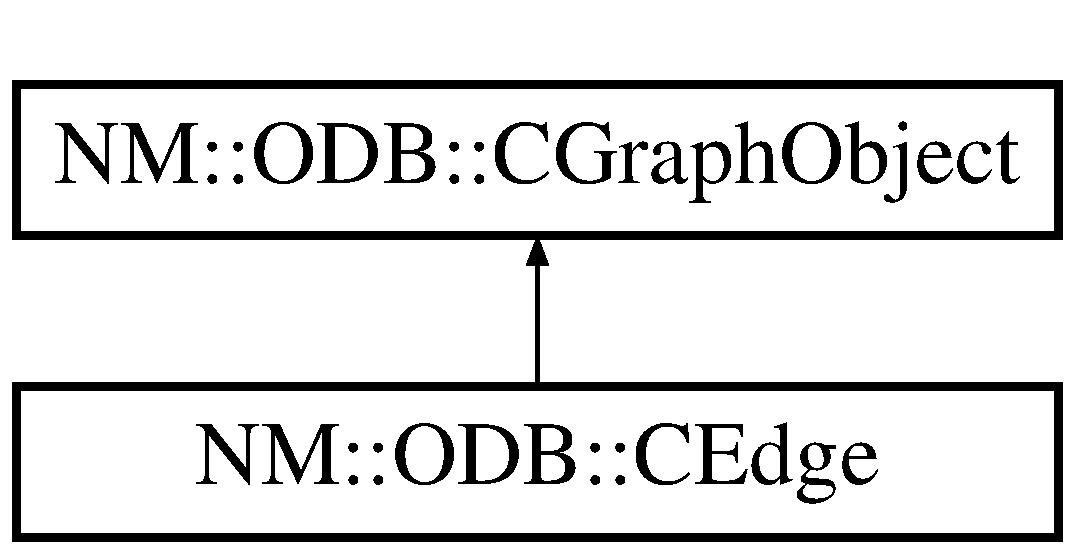
\includegraphics[height=2.000000cm]{class_n_m_1_1_o_d_b_1_1_c_edge}
\end{center}
\end{figure}
\subsection*{Public Member Functions}
\begin{DoxyCompactItemize}
\item 
\hyperlink{class_n_m_1_1_o_d_b_1_1_c_edge_a42bdb065c2e6930e580eb5ce4af7736f}{C\+Edge} ()
\item 
\hyperlink{class_n_m_1_1_o_d_b_1_1_c_edge_a40c2bd301301d32a02251a6e6051b0f1}{$\sim$\+C\+Edge} ()
\item 
\hyperlink{class_n_m_1_1_o_d_b_1_1_c_edge}{C\+Edge} $\ast$ \hyperlink{class_n_m_1_1_o_d_b_1_1_c_edge_a34f284806ef8d5ebea50011032ec1914}{clone} (size\+\_\+t new\+Object\+U\+I\+D) const 
\item 
\hyperlink{class_n_m_1_1_o_d_b_1_1_c_edge_aba180d31769a4c9205fb0f445f9d1f87}{C\+Edge} (const \hyperlink{class_n_m_1_1_o_d_b_1_1_c_edge}{C\+Edge} \&o, const \hyperlink{namespace_n_m_1_1_o_d_b_a262b64fab56baaa96e18bac4ada88265}{O\+B\+J\+E\+C\+T\+U\+I\+D} New\+U\+I\+D)
\item 
bool \hyperlink{class_n_m_1_1_o_d_b_1_1_c_edge_ad232fb24c5a0077da58e45ef8a4399b9}{Point\+In\+Object} (int \&x, int \&y)
\item 
bool \hyperlink{class_n_m_1_1_o_d_b_1_1_c_edge_a406cfa223dd80dab9ad8643848c80edc}{Point\+In\+Polygon} (int poly\+Sides, float $\ast$poly\+X, float $\ast$poly\+Y, int x, int y)
\end{DoxyCompactItemize}
\subsection*{Friends}
\begin{DoxyCompactItemize}
\item 
class \hyperlink{class_n_m_1_1_o_d_b_1_1_c_edge_afb64c52eb3833710d8b813698ec97179}{C\+Edge\+Table}
\end{DoxyCompactItemize}
\subsection*{Additional Inherited Members}


\subsection{Detailed Description}
Class \hyperlink{class_n_m_1_1_o_d_b_1_1_c_edge}{C\+Edge} 

\subsection{Constructor \& Destructor Documentation}
\hypertarget{class_n_m_1_1_o_d_b_1_1_c_edge_a42bdb065c2e6930e580eb5ce4af7736f}{}\index{N\+M\+::\+O\+D\+B\+::\+C\+Edge@{N\+M\+::\+O\+D\+B\+::\+C\+Edge}!C\+Edge@{C\+Edge}}
\index{C\+Edge@{C\+Edge}!N\+M\+::\+O\+D\+B\+::\+C\+Edge@{N\+M\+::\+O\+D\+B\+::\+C\+Edge}}
\subsubsection[{C\+Edge()}]{\setlength{\rightskip}{0pt plus 5cm}N\+M\+::\+O\+D\+B\+::\+C\+Edge\+::\+C\+Edge (
\begin{DoxyParamCaption}
{}
\end{DoxyParamCaption}
)\hspace{0.3cm}{\ttfamily [inline]}}\label{class_n_m_1_1_o_d_b_1_1_c_edge_a42bdb065c2e6930e580eb5ce4af7736f}
\hypertarget{class_n_m_1_1_o_d_b_1_1_c_edge_a40c2bd301301d32a02251a6e6051b0f1}{}\index{N\+M\+::\+O\+D\+B\+::\+C\+Edge@{N\+M\+::\+O\+D\+B\+::\+C\+Edge}!````~C\+Edge@{$\sim$\+C\+Edge}}
\index{````~C\+Edge@{$\sim$\+C\+Edge}!N\+M\+::\+O\+D\+B\+::\+C\+Edge@{N\+M\+::\+O\+D\+B\+::\+C\+Edge}}
\subsubsection[{$\sim$\+C\+Edge()}]{\setlength{\rightskip}{0pt plus 5cm}N\+M\+::\+O\+D\+B\+::\+C\+Edge\+::$\sim$\+C\+Edge (
\begin{DoxyParamCaption}
{}
\end{DoxyParamCaption}
)\hspace{0.3cm}{\ttfamily [inline]}}\label{class_n_m_1_1_o_d_b_1_1_c_edge_a40c2bd301301d32a02251a6e6051b0f1}
\hypertarget{class_n_m_1_1_o_d_b_1_1_c_edge_aba180d31769a4c9205fb0f445f9d1f87}{}\index{N\+M\+::\+O\+D\+B\+::\+C\+Edge@{N\+M\+::\+O\+D\+B\+::\+C\+Edge}!C\+Edge@{C\+Edge}}
\index{C\+Edge@{C\+Edge}!N\+M\+::\+O\+D\+B\+::\+C\+Edge@{N\+M\+::\+O\+D\+B\+::\+C\+Edge}}
\subsubsection[{C\+Edge(const C\+Edge \&o, const O\+B\+J\+E\+C\+T\+U\+I\+D New\+U\+I\+D)}]{\setlength{\rightskip}{0pt plus 5cm}N\+M\+::\+O\+D\+B\+::\+C\+Edge\+::\+C\+Edge (
\begin{DoxyParamCaption}
\item[{const {\bf C\+Edge} \&}]{o, }
\item[{const {\bf O\+B\+J\+E\+C\+T\+U\+I\+D}}]{New\+U\+I\+D}
\end{DoxyParamCaption}
)\hspace{0.3cm}{\ttfamily [inline]}}\label{class_n_m_1_1_o_d_b_1_1_c_edge_aba180d31769a4c9205fb0f445f9d1f87}


\subsection{Member Function Documentation}
\hypertarget{class_n_m_1_1_o_d_b_1_1_c_edge_a34f284806ef8d5ebea50011032ec1914}{}\index{N\+M\+::\+O\+D\+B\+::\+C\+Edge@{N\+M\+::\+O\+D\+B\+::\+C\+Edge}!clone@{clone}}
\index{clone@{clone}!N\+M\+::\+O\+D\+B\+::\+C\+Edge@{N\+M\+::\+O\+D\+B\+::\+C\+Edge}}
\subsubsection[{clone(size\+\_\+t new\+Object\+U\+I\+D) const }]{\setlength{\rightskip}{0pt plus 5cm}{\bf C\+Edge}$\ast$ N\+M\+::\+O\+D\+B\+::\+C\+Edge\+::clone (
\begin{DoxyParamCaption}
\item[{size\+\_\+t}]{new\+Object\+U\+I\+D}
\end{DoxyParamCaption}
) const\hspace{0.3cm}{\ttfamily [inline]}, {\ttfamily [virtual]}}\label{class_n_m_1_1_o_d_b_1_1_c_edge_a34f284806ef8d5ebea50011032ec1914}


Implements \hyperlink{class_n_m_1_1_o_d_b_1_1_c_graph_object_aa0ca9ee294c6b42e39fb2c3a6598b506}{N\+M\+::\+O\+D\+B\+::\+C\+Graph\+Object}.

\hypertarget{class_n_m_1_1_o_d_b_1_1_c_edge_ad232fb24c5a0077da58e45ef8a4399b9}{}\index{N\+M\+::\+O\+D\+B\+::\+C\+Edge@{N\+M\+::\+O\+D\+B\+::\+C\+Edge}!Point\+In\+Object@{Point\+In\+Object}}
\index{Point\+In\+Object@{Point\+In\+Object}!N\+M\+::\+O\+D\+B\+::\+C\+Edge@{N\+M\+::\+O\+D\+B\+::\+C\+Edge}}
\subsubsection[{Point\+In\+Object(int \&x, int \&y)}]{\setlength{\rightskip}{0pt plus 5cm}bool N\+M\+::\+O\+D\+B\+::\+C\+Edge\+::\+Point\+In\+Object (
\begin{DoxyParamCaption}
\item[{int \&}]{x, }
\item[{int \&}]{y}
\end{DoxyParamCaption}
)\hspace{0.3cm}{\ttfamily [virtual]}}\label{class_n_m_1_1_o_d_b_1_1_c_edge_ad232fb24c5a0077da58e45ef8a4399b9}


Reimplemented from \hyperlink{class_n_m_1_1_o_d_b_1_1_c_graph_object_a8069a2286005ece610484b60ee8c0fde}{N\+M\+::\+O\+D\+B\+::\+C\+Graph\+Object}.

\hypertarget{class_n_m_1_1_o_d_b_1_1_c_edge_a406cfa223dd80dab9ad8643848c80edc}{}\index{N\+M\+::\+O\+D\+B\+::\+C\+Edge@{N\+M\+::\+O\+D\+B\+::\+C\+Edge}!Point\+In\+Polygon@{Point\+In\+Polygon}}
\index{Point\+In\+Polygon@{Point\+In\+Polygon}!N\+M\+::\+O\+D\+B\+::\+C\+Edge@{N\+M\+::\+O\+D\+B\+::\+C\+Edge}}
\subsubsection[{Point\+In\+Polygon(int poly\+Sides, float $\ast$poly\+X, float $\ast$poly\+Y, int x, int y)}]{\setlength{\rightskip}{0pt plus 5cm}bool N\+M\+::\+O\+D\+B\+::\+C\+Edge\+::\+Point\+In\+Polygon (
\begin{DoxyParamCaption}
\item[{int}]{poly\+Sides, }
\item[{float $\ast$}]{poly\+X, }
\item[{float $\ast$}]{poly\+Y, }
\item[{int}]{x, }
\item[{int}]{y}
\end{DoxyParamCaption}
)}\label{class_n_m_1_1_o_d_b_1_1_c_edge_a406cfa223dd80dab9ad8643848c80edc}
Point\+In\+Polygon

int poly\+Sides = how many corners the polygon has float poly\+X\mbox{[}\mbox{]} = horizontal coordinates of corners float poly\+Y\mbox{[}\mbox{]} = vertical coordinates of corners float x, y = point to be tested 

\subsection{Friends And Related Function Documentation}
\hypertarget{class_n_m_1_1_o_d_b_1_1_c_edge_afb64c52eb3833710d8b813698ec97179}{}\index{N\+M\+::\+O\+D\+B\+::\+C\+Edge@{N\+M\+::\+O\+D\+B\+::\+C\+Edge}!C\+Edge\+Table@{C\+Edge\+Table}}
\index{C\+Edge\+Table@{C\+Edge\+Table}!N\+M\+::\+O\+D\+B\+::\+C\+Edge@{N\+M\+::\+O\+D\+B\+::\+C\+Edge}}
\subsubsection[{C\+Edge\+Table}]{\setlength{\rightskip}{0pt plus 5cm}friend class {\bf C\+Edge\+Table}\hspace{0.3cm}{\ttfamily [friend]}}\label{class_n_m_1_1_o_d_b_1_1_c_edge_afb64c52eb3833710d8b813698ec97179}


The documentation for this class was generated from the following files\+:\begin{DoxyCompactItemize}
\item 
C\+:/\+Users/\+Simon/\+Documents/\+Personal/\+Source Code/\+Projects/\+Network\+Modeller/\+Object\+Database/\+Data\+Objects/\hyperlink{_graph_objects_8h}{Graph\+Objects.\+h}\item 
C\+:/\+Users/\+Simon/\+Documents/\+Personal/\+Source Code/\+Projects/\+Network\+Modeller/\+Object\+Database/\+Data\+Objects/\hyperlink{_graph_objects_8cpp}{Graph\+Objects.\+cpp}\end{DoxyCompactItemize}

\hypertarget{class_n_m_1_1_o_d_b_1_1_c_edge_table}{}\section{N\+M\+:\+:O\+D\+B\+:\+:C\+Edge\+Table Class Reference}
\label{class_n_m_1_1_o_d_b_1_1_c_edge_table}\index{N\+M\+::\+O\+D\+B\+::\+C\+Edge\+Table@{N\+M\+::\+O\+D\+B\+::\+C\+Edge\+Table}}


{\ttfamily \#include $<$Edge\+Table.\+h$>$}

Inheritance diagram for N\+M\+:\+:O\+D\+B\+:\+:C\+Edge\+Table\+:\begin{figure}[H]
\begin{center}
\leavevmode
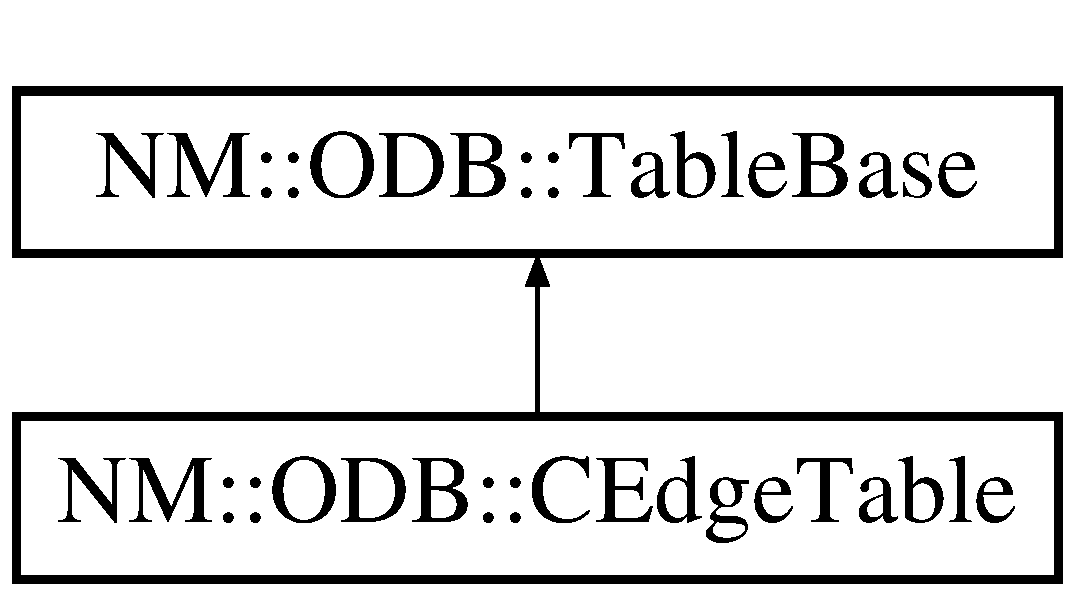
\includegraphics[height=2.000000cm]{class_n_m_1_1_o_d_b_1_1_c_edge_table}
\end{center}
\end{figure}
\subsection*{Public Types}
\begin{DoxyCompactItemize}
\item 
typedef \+::std\+::vector$<$ \hyperlink{class_n_m_1_1_o_d_b_1_1_c_graph_object}{C\+Graph\+Object} $\ast$ $>$ \hyperlink{class_n_m_1_1_o_d_b_1_1_c_edge_table_acb09088dea6dd356999095d7c7cb977a}{E\+D\+G\+E\+\_\+\+V\+E\+C\+T\+O\+R}
\end{DoxyCompactItemize}
\subsection*{Public Member Functions}
\begin{DoxyCompactItemize}
\item 
\hyperlink{class_n_m_1_1_o_d_b_1_1_c_edge_table_a6f43fd9cd4bbdb2a70652059195e94f3}{C\+Edge\+Table} (\hyperlink{class_n_m_1_1_o_d_b_1_1_c_graph_object_factory}{C\+Graph\+Object\+Factory} $\ast$object\+Factory)
\item 
\hyperlink{class_n_m_1_1_o_d_b_1_1_c_edge_table_ab18a394e7956aba0a7791c8306a0da7d}{$\sim$\+C\+Edge\+Table} (void)
\item 
\hyperlink{namespace_n_m_1_1_o_d_b_a262b64fab56baaa96e18bac4ada88265}{O\+B\+J\+E\+C\+T\+U\+I\+D} \hyperlink{class_n_m_1_1_o_d_b_1_1_c_edge_table_ada23e934605fb03751af8c8f0d103586}{Create\+Edge} (\hyperlink{namespace_n_m_1_1_o_d_b_a8770283da9792324e1afe8104d40123b}{O\+B\+J\+E\+C\+T\+A\+T\+T\+R\+I\+B\+U\+T\+E\+S} $\ast$attribute\+Map I\+N, \hyperlink{class_n_m_1_1_o_d_b_1_1_c_graph_object}{C\+Graph\+Object} $\ast$$\ast$p\+Object O\+U\+T)
\item 
bool \hyperlink{class_n_m_1_1_o_d_b_1_1_c_edge_table_a0f87540d83e5e271b03bef2923c7ee24}{Destroy\+Edge} (\hyperlink{class_n_m_1_1_o_d_b_1_1_c_graph_object}{C\+Graph\+Object} $\ast$p\+Object)
\item 
void \hyperlink{class_n_m_1_1_o_d_b_1_1_c_edge_table_a8415e1e3d9b141b70b1f070da70496f4}{Clear} (void)
\item 
\hyperlink{namespace_n_m_1_1_o_d_b_a262b64fab56baaa96e18bac4ada88265}{O\+B\+J\+E\+C\+T\+U\+I\+D} \hyperlink{class_n_m_1_1_o_d_b_1_1_c_edge_table_a5a6d28ed886386af18efec130eb0307c}{Is\+In\+Edge} (int x, int y)
\item 
bool \hyperlink{class_n_m_1_1_o_d_b_1_1_c_edge_table_a67f722668bfebd46ac05288e20523003}{Set\+Value} (\hyperlink{class_n_m_1_1_o_d_b_1_1_c_graph_object}{C\+Graph\+Object} $\ast$, size\+\_\+t idx, \hyperlink{class_n_m_1_1_o_d_b_1_1_value}{Value} const \&v)
\item 
bool \hyperlink{class_n_m_1_1_o_d_b_1_1_c_edge_table_ad210f2bbf1ba2c9e3a314814a8c1df9e}{Set\+Value} (\hyperlink{class_n_m_1_1_o_d_b_1_1_c_graph_object}{C\+Graph\+Object} $\ast$, const \+::std\+::wstring \&attrname, \hyperlink{class_n_m_1_1_o_d_b_1_1_value}{Value} const \&v)
\end{DoxyCompactItemize}
\subsection*{Public Attributes}
\begin{DoxyCompactItemize}
\item 
\hyperlink{class_n_m_1_1_o_d_b_1_1_c_edge_table_acb09088dea6dd356999095d7c7cb977a}{E\+D\+G\+E\+\_\+\+V\+E\+C\+T\+O\+R} \hyperlink{class_n_m_1_1_o_d_b_1_1_c_edge_table_a13626344aef11255b5c5e3538613854f}{edges}
\end{DoxyCompactItemize}
\subsection*{Friends}
\begin{DoxyCompactItemize}
\item 
class \hyperlink{class_n_m_1_1_o_d_b_1_1_c_edge_table_a8451ee9e81bc51a04afb10dc6ee7e07e}{C\+Object\+Database}
\end{DoxyCompactItemize}


\subsection{Member Typedef Documentation}
\hypertarget{class_n_m_1_1_o_d_b_1_1_c_edge_table_acb09088dea6dd356999095d7c7cb977a}{}\index{N\+M\+::\+O\+D\+B\+::\+C\+Edge\+Table@{N\+M\+::\+O\+D\+B\+::\+C\+Edge\+Table}!E\+D\+G\+E\+\_\+\+V\+E\+C\+T\+O\+R@{E\+D\+G\+E\+\_\+\+V\+E\+C\+T\+O\+R}}
\index{E\+D\+G\+E\+\_\+\+V\+E\+C\+T\+O\+R@{E\+D\+G\+E\+\_\+\+V\+E\+C\+T\+O\+R}!N\+M\+::\+O\+D\+B\+::\+C\+Edge\+Table@{N\+M\+::\+O\+D\+B\+::\+C\+Edge\+Table}}
\subsubsection[{E\+D\+G\+E\+\_\+\+V\+E\+C\+T\+O\+R}]{\setlength{\rightskip}{0pt plus 5cm}typedef \+::std\+::vector$<${\bf C\+Graph\+Object}$\ast$$>$ {\bf N\+M\+::\+O\+D\+B\+::\+C\+Edge\+Table\+::\+E\+D\+G\+E\+\_\+\+V\+E\+C\+T\+O\+R}}\label{class_n_m_1_1_o_d_b_1_1_c_edge_table_acb09088dea6dd356999095d7c7cb977a}


\subsection{Constructor \& Destructor Documentation}
\hypertarget{class_n_m_1_1_o_d_b_1_1_c_edge_table_a6f43fd9cd4bbdb2a70652059195e94f3}{}\index{N\+M\+::\+O\+D\+B\+::\+C\+Edge\+Table@{N\+M\+::\+O\+D\+B\+::\+C\+Edge\+Table}!C\+Edge\+Table@{C\+Edge\+Table}}
\index{C\+Edge\+Table@{C\+Edge\+Table}!N\+M\+::\+O\+D\+B\+::\+C\+Edge\+Table@{N\+M\+::\+O\+D\+B\+::\+C\+Edge\+Table}}
\subsubsection[{C\+Edge\+Table(\+C\+Graph\+Object\+Factory $\ast$object\+Factory)}]{\setlength{\rightskip}{0pt plus 5cm}N\+M\+::\+O\+D\+B\+::\+C\+Edge\+Table\+::\+C\+Edge\+Table (
\begin{DoxyParamCaption}
\item[{{\bf C\+Graph\+Object\+Factory} $\ast$}]{object\+Factory}
\end{DoxyParamCaption}
)\hspace{0.3cm}{\ttfamily [explicit]}}\label{class_n_m_1_1_o_d_b_1_1_c_edge_table_a6f43fd9cd4bbdb2a70652059195e94f3}
\hypertarget{class_n_m_1_1_o_d_b_1_1_c_edge_table_ab18a394e7956aba0a7791c8306a0da7d}{}\index{N\+M\+::\+O\+D\+B\+::\+C\+Edge\+Table@{N\+M\+::\+O\+D\+B\+::\+C\+Edge\+Table}!````~C\+Edge\+Table@{$\sim$\+C\+Edge\+Table}}
\index{````~C\+Edge\+Table@{$\sim$\+C\+Edge\+Table}!N\+M\+::\+O\+D\+B\+::\+C\+Edge\+Table@{N\+M\+::\+O\+D\+B\+::\+C\+Edge\+Table}}
\subsubsection[{$\sim$\+C\+Edge\+Table(void)}]{\setlength{\rightskip}{0pt plus 5cm}N\+M\+::\+O\+D\+B\+::\+C\+Edge\+Table\+::$\sim$\+C\+Edge\+Table (
\begin{DoxyParamCaption}
\item[{void}]{}
\end{DoxyParamCaption}
)}\label{class_n_m_1_1_o_d_b_1_1_c_edge_table_ab18a394e7956aba0a7791c8306a0da7d}


\subsection{Member Function Documentation}
\hypertarget{class_n_m_1_1_o_d_b_1_1_c_edge_table_a8415e1e3d9b141b70b1f070da70496f4}{}\index{N\+M\+::\+O\+D\+B\+::\+C\+Edge\+Table@{N\+M\+::\+O\+D\+B\+::\+C\+Edge\+Table}!Clear@{Clear}}
\index{Clear@{Clear}!N\+M\+::\+O\+D\+B\+::\+C\+Edge\+Table@{N\+M\+::\+O\+D\+B\+::\+C\+Edge\+Table}}
\subsubsection[{Clear(void)}]{\setlength{\rightskip}{0pt plus 5cm}void N\+M\+::\+O\+D\+B\+::\+C\+Edge\+Table\+::\+Clear (
\begin{DoxyParamCaption}
\item[{void}]{}
\end{DoxyParamCaption}
)}\label{class_n_m_1_1_o_d_b_1_1_c_edge_table_a8415e1e3d9b141b70b1f070da70496f4}
\hypertarget{class_n_m_1_1_o_d_b_1_1_c_edge_table_ada23e934605fb03751af8c8f0d103586}{}\index{N\+M\+::\+O\+D\+B\+::\+C\+Edge\+Table@{N\+M\+::\+O\+D\+B\+::\+C\+Edge\+Table}!Create\+Edge@{Create\+Edge}}
\index{Create\+Edge@{Create\+Edge}!N\+M\+::\+O\+D\+B\+::\+C\+Edge\+Table@{N\+M\+::\+O\+D\+B\+::\+C\+Edge\+Table}}
\subsubsection[{Create\+Edge(\+O\+B\+J\+E\+C\+T\+A\+T\+T\+R\+I\+B\+U\+T\+E\+S $\ast$attribute\+Map I\+N, C\+Graph\+Object $\ast$$\ast$p\+Object O\+U\+T)}]{\setlength{\rightskip}{0pt plus 5cm}{\bf O\+B\+J\+E\+C\+T\+U\+I\+D} N\+M\+::\+O\+D\+B\+::\+C\+Edge\+Table\+::\+Create\+Edge (
\begin{DoxyParamCaption}
\item[{{\bf O\+B\+J\+E\+C\+T\+A\+T\+T\+R\+I\+B\+U\+T\+E\+S} $\ast$attribute\+Map}]{I\+N, }
\item[{{\bf C\+Graph\+Object} $\ast$$\ast$p\+Object}]{O\+U\+T}
\end{DoxyParamCaption}
)}\label{class_n_m_1_1_o_d_b_1_1_c_edge_table_ada23e934605fb03751af8c8f0d103586}
\hypertarget{class_n_m_1_1_o_d_b_1_1_c_edge_table_a0f87540d83e5e271b03bef2923c7ee24}{}\index{N\+M\+::\+O\+D\+B\+::\+C\+Edge\+Table@{N\+M\+::\+O\+D\+B\+::\+C\+Edge\+Table}!Destroy\+Edge@{Destroy\+Edge}}
\index{Destroy\+Edge@{Destroy\+Edge}!N\+M\+::\+O\+D\+B\+::\+C\+Edge\+Table@{N\+M\+::\+O\+D\+B\+::\+C\+Edge\+Table}}
\subsubsection[{Destroy\+Edge(\+C\+Graph\+Object $\ast$p\+Object)}]{\setlength{\rightskip}{0pt plus 5cm}bool N\+M\+::\+O\+D\+B\+::\+C\+Edge\+Table\+::\+Destroy\+Edge (
\begin{DoxyParamCaption}
\item[{{\bf C\+Graph\+Object} $\ast$}]{p\+Object}
\end{DoxyParamCaption}
)}\label{class_n_m_1_1_o_d_b_1_1_c_edge_table_a0f87540d83e5e271b03bef2923c7ee24}
\hypertarget{class_n_m_1_1_o_d_b_1_1_c_edge_table_a5a6d28ed886386af18efec130eb0307c}{}\index{N\+M\+::\+O\+D\+B\+::\+C\+Edge\+Table@{N\+M\+::\+O\+D\+B\+::\+C\+Edge\+Table}!Is\+In\+Edge@{Is\+In\+Edge}}
\index{Is\+In\+Edge@{Is\+In\+Edge}!N\+M\+::\+O\+D\+B\+::\+C\+Edge\+Table@{N\+M\+::\+O\+D\+B\+::\+C\+Edge\+Table}}
\subsubsection[{Is\+In\+Edge(int x, int y)}]{\setlength{\rightskip}{0pt plus 5cm}{\bf O\+B\+J\+E\+C\+T\+U\+I\+D} N\+M\+::\+O\+D\+B\+::\+C\+Edge\+Table\+::\+Is\+In\+Edge (
\begin{DoxyParamCaption}
\item[{int}]{x, }
\item[{int}]{y}
\end{DoxyParamCaption}
)}\label{class_n_m_1_1_o_d_b_1_1_c_edge_table_a5a6d28ed886386af18efec130eb0307c}
Is\+In\+Edge -\/ needs to be moved outside of Edge\+Table (Edge\+Table) so its not having to access Object\+Database -\/ should be autonomous \hypertarget{class_n_m_1_1_o_d_b_1_1_c_edge_table_a67f722668bfebd46ac05288e20523003}{}\index{N\+M\+::\+O\+D\+B\+::\+C\+Edge\+Table@{N\+M\+::\+O\+D\+B\+::\+C\+Edge\+Table}!Set\+Value@{Set\+Value}}
\index{Set\+Value@{Set\+Value}!N\+M\+::\+O\+D\+B\+::\+C\+Edge\+Table@{N\+M\+::\+O\+D\+B\+::\+C\+Edge\+Table}}
\subsubsection[{Set\+Value(\+C\+Graph\+Object $\ast$, size\+\_\+t idx, Value const \&v)}]{\setlength{\rightskip}{0pt plus 5cm}bool N\+M\+::\+O\+D\+B\+::\+C\+Edge\+Table\+::\+Set\+Value (
\begin{DoxyParamCaption}
\item[{{\bf C\+Graph\+Object} $\ast$}]{edge, }
\item[{size\+\_\+t}]{idx, }
\item[{{\bf Value} const \&}]{v}
\end{DoxyParamCaption}
)\hspace{0.3cm}{\ttfamily [virtual]}}\label{class_n_m_1_1_o_d_b_1_1_c_edge_table_a67f722668bfebd46ac05288e20523003}


Implements \hyperlink{class_n_m_1_1_o_d_b_1_1_table_base_afbc340c36e140f2a8184d2585cc3b5d5}{N\+M\+::\+O\+D\+B\+::\+Table\+Base}.

\hypertarget{class_n_m_1_1_o_d_b_1_1_c_edge_table_ad210f2bbf1ba2c9e3a314814a8c1df9e}{}\index{N\+M\+::\+O\+D\+B\+::\+C\+Edge\+Table@{N\+M\+::\+O\+D\+B\+::\+C\+Edge\+Table}!Set\+Value@{Set\+Value}}
\index{Set\+Value@{Set\+Value}!N\+M\+::\+O\+D\+B\+::\+C\+Edge\+Table@{N\+M\+::\+O\+D\+B\+::\+C\+Edge\+Table}}
\subsubsection[{Set\+Value(\+C\+Graph\+Object $\ast$, const \+::std\+::wstring \&attrname, Value const \&v)}]{\setlength{\rightskip}{0pt plus 5cm}bool N\+M\+::\+O\+D\+B\+::\+C\+Edge\+Table\+::\+Set\+Value (
\begin{DoxyParamCaption}
\item[{{\bf C\+Graph\+Object} $\ast$}]{edge, }
\item[{const \+::std\+::wstring \&}]{attrname, }
\item[{{\bf Value} const \&}]{v}
\end{DoxyParamCaption}
)\hspace{0.3cm}{\ttfamily [virtual]}}\label{class_n_m_1_1_o_d_b_1_1_c_edge_table_ad210f2bbf1ba2c9e3a314814a8c1df9e}


Implements \hyperlink{class_n_m_1_1_o_d_b_1_1_table_base_a3e55bfe64ccdf81e6a96941b3f9a5fb4}{N\+M\+::\+O\+D\+B\+::\+Table\+Base}.



\subsection{Friends And Related Function Documentation}
\hypertarget{class_n_m_1_1_o_d_b_1_1_c_edge_table_a8451ee9e81bc51a04afb10dc6ee7e07e}{}\index{N\+M\+::\+O\+D\+B\+::\+C\+Edge\+Table@{N\+M\+::\+O\+D\+B\+::\+C\+Edge\+Table}!C\+Object\+Database@{C\+Object\+Database}}
\index{C\+Object\+Database@{C\+Object\+Database}!N\+M\+::\+O\+D\+B\+::\+C\+Edge\+Table@{N\+M\+::\+O\+D\+B\+::\+C\+Edge\+Table}}
\subsubsection[{C\+Object\+Database}]{\setlength{\rightskip}{0pt plus 5cm}friend class {\bf C\+Object\+Database}\hspace{0.3cm}{\ttfamily [friend]}}\label{class_n_m_1_1_o_d_b_1_1_c_edge_table_a8451ee9e81bc51a04afb10dc6ee7e07e}


\subsection{Member Data Documentation}
\hypertarget{class_n_m_1_1_o_d_b_1_1_c_edge_table_a13626344aef11255b5c5e3538613854f}{}\index{N\+M\+::\+O\+D\+B\+::\+C\+Edge\+Table@{N\+M\+::\+O\+D\+B\+::\+C\+Edge\+Table}!edges@{edges}}
\index{edges@{edges}!N\+M\+::\+O\+D\+B\+::\+C\+Edge\+Table@{N\+M\+::\+O\+D\+B\+::\+C\+Edge\+Table}}
\subsubsection[{edges}]{\setlength{\rightskip}{0pt plus 5cm}{\bf E\+D\+G\+E\+\_\+\+V\+E\+C\+T\+O\+R} N\+M\+::\+O\+D\+B\+::\+C\+Edge\+Table\+::edges}\label{class_n_m_1_1_o_d_b_1_1_c_edge_table_a13626344aef11255b5c5e3538613854f}


The documentation for this class was generated from the following files\+:\begin{DoxyCompactItemize}
\item 
C\+:/\+Users/\+Simon/\+Documents/\+Personal/\+Source Code/\+Projects/\+Network\+Modeller/\+Object\+Database/\+Tables/\hyperlink{_edge_table_8h}{Edge\+Table.\+h}\item 
C\+:/\+Users/\+Simon/\+Documents/\+Personal/\+Source Code/\+Projects/\+Network\+Modeller/\+Object\+Database/\+Tables/\hyperlink{_edge_table_8cpp}{Edge\+Table.\+cpp}\end{DoxyCompactItemize}

\hypertarget{class_n_m_1_1_o_d_b_1_1_c_graph_object}{}\section{N\+M\+:\+:O\+D\+B\+:\+:C\+Graph\+Object Class Reference}
\label{class_n_m_1_1_o_d_b_1_1_c_graph_object}\index{N\+M\+::\+O\+D\+B\+::\+C\+Graph\+Object@{N\+M\+::\+O\+D\+B\+::\+C\+Graph\+Object}}


{\ttfamily \#include $<$Graph\+Objects.\+h$>$}

Inheritance diagram for N\+M\+:\+:O\+D\+B\+:\+:C\+Graph\+Object\+:\begin{figure}[H]
\begin{center}
\leavevmode
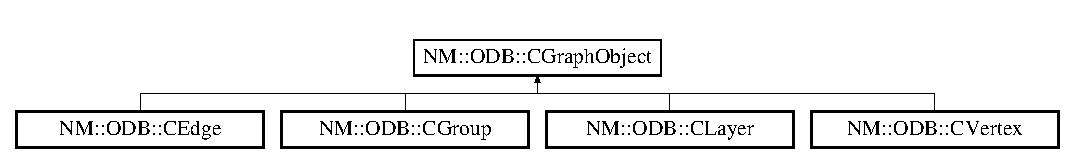
\includegraphics[height=1.750000cm]{class_n_m_1_1_o_d_b_1_1_c_graph_object}
\end{center}
\end{figure}
\subsection*{Public Member Functions}
\begin{DoxyCompactItemize}
\item 
\hyperlink{class_n_m_1_1_o_d_b_1_1_c_graph_object_a06700df2a7c050d93b0accd0e8642369}{C\+Graph\+Object} (\+::std\+::wstring objecttypename, \hyperlink{namespace_n_m_1_1_o_d_b_ac9f60beb4a1c8a6240dd0c8baa281345}{Object\+Type} object\+\_\+type)
\item 
\hyperlink{class_n_m_1_1_o_d_b_1_1_c_graph_object_ae80b46a15e4d793e295f5ee02f66cfe4}{$\sim$\+C\+Graph\+Object} ()
\item 
\hyperlink{class_n_m_1_1_o_d_b_1_1_c_graph_object_a6f43040764eb9614235394fd7054a999}{C\+Graph\+Object} (const \hyperlink{class_n_m_1_1_o_d_b_1_1_c_graph_object}{C\+Graph\+Object} \&object\+\_\+to\+\_\+copy, \hyperlink{namespace_n_m_1_1_o_d_b_a262b64fab56baaa96e18bac4ada88265}{O\+B\+J\+E\+C\+T\+U\+I\+D} new\+U\+I\+D)
\item 
virtual \hyperlink{class_n_m_1_1_o_d_b_1_1_c_graph_object}{C\+Graph\+Object} $\ast$ \hyperlink{class_n_m_1_1_o_d_b_1_1_c_graph_object_aa0ca9ee294c6b42e39fb2c3a6598b506}{clone} (size\+\_\+t new\+Object\+U\+I\+D) const  =0
\item 
virtual bool \hyperlink{class_n_m_1_1_o_d_b_1_1_c_graph_object_a8069a2286005ece610484b60ee8c0fde}{Point\+In\+Object} (int \&x, int \&y)
\item 
void \hyperlink{class_n_m_1_1_o_d_b_1_1_c_graph_object_a32778b91aca24bf7e1f1d06799e7e3c8}{Set\+Modified\+Flag} (bool bmodified)
\item 
bool \hyperlink{class_n_m_1_1_o_d_b_1_1_c_graph_object_ad8daa62d38568f2cc4742245b0b81b20}{Get\+Modified\+Flag} ()
\item 
size\+\_\+t \hyperlink{class_n_m_1_1_o_d_b_1_1_c_graph_object_a8a85ff3c3d04bab0a6affed34c5acfec}{Get\+Attribute\+Count} ()
\item 
void \hyperlink{class_n_m_1_1_o_d_b_1_1_c_graph_object_a60189d19350f322cf73dfa36559bf7d5}{Get\+Attribute\+List} (\hyperlink{namespace_n_m_1_1_o_d_b_a3c1c138c7d11b589aaa8863b6a8c1317}{Attribute\+Filter} attribute\+Filter,\+::std\+::list$<$\+::std\+::wstring $>$ \&attrlist)
\item 
bool \hyperlink{class_n_m_1_1_o_d_b_1_1_c_graph_object_a8c03cd8831fb6912dbfaa8aad56c424b}{Insert\+Attribute} (\hyperlink{class_n_m_1_1_o_d_b_1_1_attribute}{Attribute} attribute)
\item 
bool \hyperlink{class_n_m_1_1_o_d_b_1_1_c_graph_object_a204a1a4e1c62ea074aa0e3183a031759}{Is\+Attribute} (const \+::std\+::wstring \&attrname)
\item 
int \hyperlink{class_n_m_1_1_o_d_b_1_1_c_graph_object_a5d3cc425d5b4d482ee94936f9224670d}{Find\+Attribute} (const \+::std\+::wstring \&attrname)
\item 
bool \hyperlink{class_n_m_1_1_o_d_b_1_1_c_graph_object_ac6caa398d4ff96211a0e704c77da7739}{Is\+Required\+Attribute} (const \+::std\+::wstring \&attrname)
\item 
\hyperlink{class_n_m_1_1_o_d_b_1_1_attribute}{Attribute} const \& \hyperlink{class_n_m_1_1_o_d_b_1_1_c_graph_object_a291fcbb04bfa5fb1ad20535ffa6001fc}{Get\+Attribute} (size\+\_\+t attribute\+Index) const 
\item 
\hyperlink{class_n_m_1_1_o_d_b_1_1_attribute}{Attribute} const \& \hyperlink{class_n_m_1_1_o_d_b_1_1_c_graph_object_a1e1680665f362ad704ae39061e43de9f}{operator\mbox{[}$\,$\mbox{]}} (size\+\_\+t attribute\+Index) const 
\item 
\hyperlink{class_n_m_1_1_o_d_b_1_1_value}{Value} \hyperlink{class_n_m_1_1_o_d_b_1_1_c_graph_object_ab6c7879bcf22d59445eb237d9b8ce246}{Get\+Value} (size\+\_\+t attribute\+Index) const 
\item 
\hyperlink{class_n_m_1_1_o_d_b_1_1_value}{Value} \hyperlink{class_n_m_1_1_o_d_b_1_1_c_graph_object_aea1695fee8940d9c6a97b9d647d87c2c}{Get\+Value} (const \+::std\+::wstring \&attrname)
\item 
\+::std\+::wstring \hyperlink{class_n_m_1_1_o_d_b_1_1_c_graph_object_a6295db63db8cee39492f6c955078b605}{Get\+W\+String\+Value} (size\+\_\+t attribute\+Index)
\item 
\+::std\+::wstring \hyperlink{class_n_m_1_1_o_d_b_1_1_c_graph_object_ae848454b3bcb590d24b7cbe864f8eaaa}{Get\+Object\+Type\+Name} ()
\item 
\hyperlink{namespace_n_m_1_1_o_d_b_ac9f60beb4a1c8a6240dd0c8baa281345}{Object\+Type} \hyperlink{class_n_m_1_1_o_d_b_1_1_c_graph_object_ab0da8988916c6c8e2376f0c0e4ae22df}{Get\+Object\+Type} ()
\end{DoxyCompactItemize}
\subsection*{Protected Member Functions}
\begin{DoxyCompactItemize}
\item 
bool \hyperlink{class_n_m_1_1_o_d_b_1_1_c_graph_object_a08b23d43253a196f369b8563eb113f94}{Set\+Value} (size\+\_\+t attribute\+Index, \hyperlink{class_n_m_1_1_o_d_b_1_1_value}{Value} const \&v)
\item 
bool \hyperlink{class_n_m_1_1_o_d_b_1_1_c_graph_object_afacbf41e9fb2e87d5aeaaa8b46259815}{Set\+Value} (const \+::std\+::wstring \&attrname, \hyperlink{class_n_m_1_1_o_d_b_1_1_value}{Value} const \&v)
\item 
bool \hyperlink{class_n_m_1_1_o_d_b_1_1_c_graph_object_a857d52bf7ad89fdcef601721eaeb627b}{Set\+Value} (const \+::std\+::wstring \&attrname, const \+::std\+::wstring strvalue)
\end{DoxyCompactItemize}


\subsection{Detailed Description}
Class \hyperlink{class_n_m_1_1_o_d_b_1_1_c_graph_object}{C\+Graph\+Object} 

\subsection{Constructor \& Destructor Documentation}
\hypertarget{class_n_m_1_1_o_d_b_1_1_c_graph_object_a06700df2a7c050d93b0accd0e8642369}{}\index{N\+M\+::\+O\+D\+B\+::\+C\+Graph\+Object@{N\+M\+::\+O\+D\+B\+::\+C\+Graph\+Object}!C\+Graph\+Object@{C\+Graph\+Object}}
\index{C\+Graph\+Object@{C\+Graph\+Object}!N\+M\+::\+O\+D\+B\+::\+C\+Graph\+Object@{N\+M\+::\+O\+D\+B\+::\+C\+Graph\+Object}}
\subsubsection[{C\+Graph\+Object(\+::std\+::wstring objecttypename, Object\+Type object\+\_\+type)}]{\setlength{\rightskip}{0pt plus 5cm}N\+M\+::\+O\+D\+B\+::\+C\+Graph\+Object\+::\+C\+Graph\+Object (
\begin{DoxyParamCaption}
\item[{\+::std\+::wstring}]{objecttypename, }
\item[{{\bf Object\+Type}}]{objecttype}
\end{DoxyParamCaption}
)}\label{class_n_m_1_1_o_d_b_1_1_c_graph_object_a06700df2a7c050d93b0accd0e8642369}
\hyperlink{class_n_m_1_1_o_d_b_1_1_c_graph_object}{C\+Graph\+Object} \hypertarget{class_n_m_1_1_o_d_b_1_1_c_graph_object_ae80b46a15e4d793e295f5ee02f66cfe4}{}\index{N\+M\+::\+O\+D\+B\+::\+C\+Graph\+Object@{N\+M\+::\+O\+D\+B\+::\+C\+Graph\+Object}!````~C\+Graph\+Object@{$\sim$\+C\+Graph\+Object}}
\index{````~C\+Graph\+Object@{$\sim$\+C\+Graph\+Object}!N\+M\+::\+O\+D\+B\+::\+C\+Graph\+Object@{N\+M\+::\+O\+D\+B\+::\+C\+Graph\+Object}}
\subsubsection[{$\sim$\+C\+Graph\+Object()}]{\setlength{\rightskip}{0pt plus 5cm}N\+M\+::\+O\+D\+B\+::\+C\+Graph\+Object\+::$\sim$\+C\+Graph\+Object (
\begin{DoxyParamCaption}
{}
\end{DoxyParamCaption}
)}\label{class_n_m_1_1_o_d_b_1_1_c_graph_object_ae80b46a15e4d793e295f5ee02f66cfe4}
$\sim$\+C\+Graph\+Object \hypertarget{class_n_m_1_1_o_d_b_1_1_c_graph_object_a6f43040764eb9614235394fd7054a999}{}\index{N\+M\+::\+O\+D\+B\+::\+C\+Graph\+Object@{N\+M\+::\+O\+D\+B\+::\+C\+Graph\+Object}!C\+Graph\+Object@{C\+Graph\+Object}}
\index{C\+Graph\+Object@{C\+Graph\+Object}!N\+M\+::\+O\+D\+B\+::\+C\+Graph\+Object@{N\+M\+::\+O\+D\+B\+::\+C\+Graph\+Object}}
\subsubsection[{C\+Graph\+Object(const C\+Graph\+Object \&object\+\_\+to\+\_\+copy, O\+B\+J\+E\+C\+T\+U\+I\+D new\+U\+I\+D)}]{\setlength{\rightskip}{0pt plus 5cm}N\+M\+::\+O\+D\+B\+::\+C\+Graph\+Object\+::\+C\+Graph\+Object (
\begin{DoxyParamCaption}
\item[{const {\bf C\+Graph\+Object} \&}]{object\+\_\+to\+\_\+copy, }
\item[{{\bf O\+B\+J\+E\+C\+T\+U\+I\+D}}]{new\+U\+I\+D}
\end{DoxyParamCaption}
)}\label{class_n_m_1_1_o_d_b_1_1_c_graph_object_a6f43040764eb9614235394fd7054a999}
\hyperlink{class_n_m_1_1_o_d_b_1_1_c_graph_object}{C\+Graph\+Object} Copy Constructor 

\subsection{Member Function Documentation}
\hypertarget{class_n_m_1_1_o_d_b_1_1_c_graph_object_aa0ca9ee294c6b42e39fb2c3a6598b506}{}\index{N\+M\+::\+O\+D\+B\+::\+C\+Graph\+Object@{N\+M\+::\+O\+D\+B\+::\+C\+Graph\+Object}!clone@{clone}}
\index{clone@{clone}!N\+M\+::\+O\+D\+B\+::\+C\+Graph\+Object@{N\+M\+::\+O\+D\+B\+::\+C\+Graph\+Object}}
\subsubsection[{clone(size\+\_\+t new\+Object\+U\+I\+D) const  =0}]{\setlength{\rightskip}{0pt plus 5cm}virtual {\bf C\+Graph\+Object}$\ast$ N\+M\+::\+O\+D\+B\+::\+C\+Graph\+Object\+::clone (
\begin{DoxyParamCaption}
\item[{size\+\_\+t}]{new\+Object\+U\+I\+D}
\end{DoxyParamCaption}
) const\hspace{0.3cm}{\ttfamily [pure virtual]}}\label{class_n_m_1_1_o_d_b_1_1_c_graph_object_aa0ca9ee294c6b42e39fb2c3a6598b506}


Implemented in \hyperlink{class_n_m_1_1_o_d_b_1_1_c_vertex_afe1a131c1b47dc9953e5d164a380af68}{N\+M\+::\+O\+D\+B\+::\+C\+Vertex}, \hyperlink{class_n_m_1_1_o_d_b_1_1_c_group_a3e5d4ed073cad6a4ceb06cab70c84c21}{N\+M\+::\+O\+D\+B\+::\+C\+Group}, \hyperlink{class_n_m_1_1_o_d_b_1_1_c_layer_a683492260348c94f9f3660f55d1a2438}{N\+M\+::\+O\+D\+B\+::\+C\+Layer}, and \hyperlink{class_n_m_1_1_o_d_b_1_1_c_edge_a34f284806ef8d5ebea50011032ec1914}{N\+M\+::\+O\+D\+B\+::\+C\+Edge}.

\hypertarget{class_n_m_1_1_o_d_b_1_1_c_graph_object_a5d3cc425d5b4d482ee94936f9224670d}{}\index{N\+M\+::\+O\+D\+B\+::\+C\+Graph\+Object@{N\+M\+::\+O\+D\+B\+::\+C\+Graph\+Object}!Find\+Attribute@{Find\+Attribute}}
\index{Find\+Attribute@{Find\+Attribute}!N\+M\+::\+O\+D\+B\+::\+C\+Graph\+Object@{N\+M\+::\+O\+D\+B\+::\+C\+Graph\+Object}}
\subsubsection[{Find\+Attribute(const \+::std\+::wstring \&attrname)}]{\setlength{\rightskip}{0pt plus 5cm}int N\+M\+::\+O\+D\+B\+::\+C\+Graph\+Object\+::\+Find\+Attribute (
\begin{DoxyParamCaption}
\item[{const \+::std\+::wstring \&}]{attrname}
\end{DoxyParamCaption}
)}\label{class_n_m_1_1_o_d_b_1_1_c_graph_object_a5d3cc425d5b4d482ee94936f9224670d}
Find\+Attribute

find the attribute string name then return index number of the attribute \hypertarget{class_n_m_1_1_o_d_b_1_1_c_graph_object_a291fcbb04bfa5fb1ad20535ffa6001fc}{}\index{N\+M\+::\+O\+D\+B\+::\+C\+Graph\+Object@{N\+M\+::\+O\+D\+B\+::\+C\+Graph\+Object}!Get\+Attribute@{Get\+Attribute}}
\index{Get\+Attribute@{Get\+Attribute}!N\+M\+::\+O\+D\+B\+::\+C\+Graph\+Object@{N\+M\+::\+O\+D\+B\+::\+C\+Graph\+Object}}
\subsubsection[{Get\+Attribute(size\+\_\+t attribute\+Index) const }]{\setlength{\rightskip}{0pt plus 5cm}{\bf Attribute} const \& N\+M\+::\+O\+D\+B\+::\+C\+Graph\+Object\+::\+Get\+Attribute (
\begin{DoxyParamCaption}
\item[{size\+\_\+t}]{attribute\+Index}
\end{DoxyParamCaption}
) const}\label{class_n_m_1_1_o_d_b_1_1_c_graph_object_a291fcbb04bfa5fb1ad20535ffa6001fc}
Get\+Attribute

Given an valid attribute index number, return a reference to the attribute object. \hypertarget{class_n_m_1_1_o_d_b_1_1_c_graph_object_a8a85ff3c3d04bab0a6affed34c5acfec}{}\index{N\+M\+::\+O\+D\+B\+::\+C\+Graph\+Object@{N\+M\+::\+O\+D\+B\+::\+C\+Graph\+Object}!Get\+Attribute\+Count@{Get\+Attribute\+Count}}
\index{Get\+Attribute\+Count@{Get\+Attribute\+Count}!N\+M\+::\+O\+D\+B\+::\+C\+Graph\+Object@{N\+M\+::\+O\+D\+B\+::\+C\+Graph\+Object}}
\subsubsection[{Get\+Attribute\+Count()}]{\setlength{\rightskip}{0pt plus 5cm}size\+\_\+t N\+M\+::\+O\+D\+B\+::\+C\+Graph\+Object\+::\+Get\+Attribute\+Count (
\begin{DoxyParamCaption}
{}
\end{DoxyParamCaption}
)}\label{class_n_m_1_1_o_d_b_1_1_c_graph_object_a8a85ff3c3d04bab0a6affed34c5acfec}
\hypertarget{class_n_m_1_1_o_d_b_1_1_c_graph_object_a60189d19350f322cf73dfa36559bf7d5}{}\index{N\+M\+::\+O\+D\+B\+::\+C\+Graph\+Object@{N\+M\+::\+O\+D\+B\+::\+C\+Graph\+Object}!Get\+Attribute\+List@{Get\+Attribute\+List}}
\index{Get\+Attribute\+List@{Get\+Attribute\+List}!N\+M\+::\+O\+D\+B\+::\+C\+Graph\+Object@{N\+M\+::\+O\+D\+B\+::\+C\+Graph\+Object}}
\subsubsection[{Get\+Attribute\+List(\+Attribute\+Filter attribute\+Filter,\+::std\+::list$<$\+::std\+::wstring $>$ \&attrlist)}]{\setlength{\rightskip}{0pt plus 5cm}void N\+M\+::\+O\+D\+B\+::\+C\+Graph\+Object\+::\+Get\+Attribute\+List (
\begin{DoxyParamCaption}
\item[{{\bf Attribute\+Filter}}]{attribute\+Filter, }
\item[{\+::std\+::list$<$\+::std\+::wstring $>$ \&}]{attrlist}
\end{DoxyParamCaption}
)}\label{class_n_m_1_1_o_d_b_1_1_c_graph_object_a60189d19350f322cf73dfa36559bf7d5}
\hypertarget{class_n_m_1_1_o_d_b_1_1_c_graph_object_ad8daa62d38568f2cc4742245b0b81b20}{}\index{N\+M\+::\+O\+D\+B\+::\+C\+Graph\+Object@{N\+M\+::\+O\+D\+B\+::\+C\+Graph\+Object}!Get\+Modified\+Flag@{Get\+Modified\+Flag}}
\index{Get\+Modified\+Flag@{Get\+Modified\+Flag}!N\+M\+::\+O\+D\+B\+::\+C\+Graph\+Object@{N\+M\+::\+O\+D\+B\+::\+C\+Graph\+Object}}
\subsubsection[{Get\+Modified\+Flag()}]{\setlength{\rightskip}{0pt plus 5cm}bool N\+M\+::\+O\+D\+B\+::\+C\+Graph\+Object\+::\+Get\+Modified\+Flag (
\begin{DoxyParamCaption}
{}
\end{DoxyParamCaption}
)}\label{class_n_m_1_1_o_d_b_1_1_c_graph_object_ad8daa62d38568f2cc4742245b0b81b20}
\hypertarget{class_n_m_1_1_o_d_b_1_1_c_graph_object_ab0da8988916c6c8e2376f0c0e4ae22df}{}\index{N\+M\+::\+O\+D\+B\+::\+C\+Graph\+Object@{N\+M\+::\+O\+D\+B\+::\+C\+Graph\+Object}!Get\+Object\+Type@{Get\+Object\+Type}}
\index{Get\+Object\+Type@{Get\+Object\+Type}!N\+M\+::\+O\+D\+B\+::\+C\+Graph\+Object@{N\+M\+::\+O\+D\+B\+::\+C\+Graph\+Object}}
\subsubsection[{Get\+Object\+Type()}]{\setlength{\rightskip}{0pt plus 5cm}{\bf Object\+Type} N\+M\+::\+O\+D\+B\+::\+C\+Graph\+Object\+::\+Get\+Object\+Type (
\begin{DoxyParamCaption}
{}
\end{DoxyParamCaption}
)}\label{class_n_m_1_1_o_d_b_1_1_c_graph_object_ab0da8988916c6c8e2376f0c0e4ae22df}
\hypertarget{class_n_m_1_1_o_d_b_1_1_c_graph_object_ae848454b3bcb590d24b7cbe864f8eaaa}{}\index{N\+M\+::\+O\+D\+B\+::\+C\+Graph\+Object@{N\+M\+::\+O\+D\+B\+::\+C\+Graph\+Object}!Get\+Object\+Type\+Name@{Get\+Object\+Type\+Name}}
\index{Get\+Object\+Type\+Name@{Get\+Object\+Type\+Name}!N\+M\+::\+O\+D\+B\+::\+C\+Graph\+Object@{N\+M\+::\+O\+D\+B\+::\+C\+Graph\+Object}}
\subsubsection[{Get\+Object\+Type\+Name()}]{\setlength{\rightskip}{0pt plus 5cm}std\+::wstring N\+M\+::\+O\+D\+B\+::\+C\+Graph\+Object\+::\+Get\+Object\+Type\+Name (
\begin{DoxyParamCaption}
{}
\end{DoxyParamCaption}
)}\label{class_n_m_1_1_o_d_b_1_1_c_graph_object_ae848454b3bcb590d24b7cbe864f8eaaa}
Get\+Object\+Type\+Name

Returns this objects type as a string, i.\+e. Vertex, Edge etc \hypertarget{class_n_m_1_1_o_d_b_1_1_c_graph_object_ab6c7879bcf22d59445eb237d9b8ce246}{}\index{N\+M\+::\+O\+D\+B\+::\+C\+Graph\+Object@{N\+M\+::\+O\+D\+B\+::\+C\+Graph\+Object}!Get\+Value@{Get\+Value}}
\index{Get\+Value@{Get\+Value}!N\+M\+::\+O\+D\+B\+::\+C\+Graph\+Object@{N\+M\+::\+O\+D\+B\+::\+C\+Graph\+Object}}
\subsubsection[{Get\+Value(size\+\_\+t attribute\+Index) const }]{\setlength{\rightskip}{0pt plus 5cm}{\bf Value} N\+M\+::\+O\+D\+B\+::\+C\+Graph\+Object\+::\+Get\+Value (
\begin{DoxyParamCaption}
\item[{size\+\_\+t}]{attribute\+Index}
\end{DoxyParamCaption}
) const}\label{class_n_m_1_1_o_d_b_1_1_c_graph_object_ab6c7879bcf22d59445eb237d9b8ce246}
Get\+Value

Given an attribute index, return a copy of the \hyperlink{class_n_m_1_1_o_d_b_1_1_value}{Value} \hypertarget{class_n_m_1_1_o_d_b_1_1_c_graph_object_aea1695fee8940d9c6a97b9d647d87c2c}{}\index{N\+M\+::\+O\+D\+B\+::\+C\+Graph\+Object@{N\+M\+::\+O\+D\+B\+::\+C\+Graph\+Object}!Get\+Value@{Get\+Value}}
\index{Get\+Value@{Get\+Value}!N\+M\+::\+O\+D\+B\+::\+C\+Graph\+Object@{N\+M\+::\+O\+D\+B\+::\+C\+Graph\+Object}}
\subsubsection[{Get\+Value(const \+::std\+::wstring \&attrname)}]{\setlength{\rightskip}{0pt plus 5cm}{\bf Value} N\+M\+::\+O\+D\+B\+::\+C\+Graph\+Object\+::\+Get\+Value (
\begin{DoxyParamCaption}
\item[{const \+::std\+::wstring \&}]{attrname}
\end{DoxyParamCaption}
)}\label{class_n_m_1_1_o_d_b_1_1_c_graph_object_aea1695fee8940d9c6a97b9d647d87c2c}
Get\+Value

Given an attribute name as a string, return a copy of the \hyperlink{class_n_m_1_1_o_d_b_1_1_value}{Value} \hypertarget{class_n_m_1_1_o_d_b_1_1_c_graph_object_a6295db63db8cee39492f6c955078b605}{}\index{N\+M\+::\+O\+D\+B\+::\+C\+Graph\+Object@{N\+M\+::\+O\+D\+B\+::\+C\+Graph\+Object}!Get\+W\+String\+Value@{Get\+W\+String\+Value}}
\index{Get\+W\+String\+Value@{Get\+W\+String\+Value}!N\+M\+::\+O\+D\+B\+::\+C\+Graph\+Object@{N\+M\+::\+O\+D\+B\+::\+C\+Graph\+Object}}
\subsubsection[{Get\+W\+String\+Value(size\+\_\+t attribute\+Index)}]{\setlength{\rightskip}{0pt plus 5cm}std\+::wstring N\+M\+::\+O\+D\+B\+::\+C\+Graph\+Object\+::\+Get\+W\+String\+Value (
\begin{DoxyParamCaption}
\item[{size\+\_\+t}]{attribute\+Index}
\end{DoxyParamCaption}
)}\label{class_n_m_1_1_o_d_b_1_1_c_graph_object_a6295db63db8cee39492f6c955078b605}
Get\+W\+String\+Value

Given an attribute Index, return the attribute value as a string \hypertarget{class_n_m_1_1_o_d_b_1_1_c_graph_object_a8c03cd8831fb6912dbfaa8aad56c424b}{}\index{N\+M\+::\+O\+D\+B\+::\+C\+Graph\+Object@{N\+M\+::\+O\+D\+B\+::\+C\+Graph\+Object}!Insert\+Attribute@{Insert\+Attribute}}
\index{Insert\+Attribute@{Insert\+Attribute}!N\+M\+::\+O\+D\+B\+::\+C\+Graph\+Object@{N\+M\+::\+O\+D\+B\+::\+C\+Graph\+Object}}
\subsubsection[{Insert\+Attribute(\+Attribute attribute)}]{\setlength{\rightskip}{0pt plus 5cm}bool N\+M\+::\+O\+D\+B\+::\+C\+Graph\+Object\+::\+Insert\+Attribute (
\begin{DoxyParamCaption}
\item[{{\bf Attribute}}]{attribute}
\end{DoxyParamCaption}
)}\label{class_n_m_1_1_o_d_b_1_1_c_graph_object_a8c03cd8831fb6912dbfaa8aad56c424b}
\hypertarget{class_n_m_1_1_o_d_b_1_1_c_graph_object_a204a1a4e1c62ea074aa0e3183a031759}{}\index{N\+M\+::\+O\+D\+B\+::\+C\+Graph\+Object@{N\+M\+::\+O\+D\+B\+::\+C\+Graph\+Object}!Is\+Attribute@{Is\+Attribute}}
\index{Is\+Attribute@{Is\+Attribute}!N\+M\+::\+O\+D\+B\+::\+C\+Graph\+Object@{N\+M\+::\+O\+D\+B\+::\+C\+Graph\+Object}}
\subsubsection[{Is\+Attribute(const \+::std\+::wstring \&attrname)}]{\setlength{\rightskip}{0pt plus 5cm}bool N\+M\+::\+O\+D\+B\+::\+C\+Graph\+Object\+::\+Is\+Attribute (
\begin{DoxyParamCaption}
\item[{const \+::std\+::wstring \&}]{attrname}
\end{DoxyParamCaption}
)}\label{class_n_m_1_1_o_d_b_1_1_c_graph_object_a204a1a4e1c62ea074aa0e3183a031759}
Is\+Attribute

Given an attribute string name, if is an attribute in this object then return true, else false. \hypertarget{class_n_m_1_1_o_d_b_1_1_c_graph_object_ac6caa398d4ff96211a0e704c77da7739}{}\index{N\+M\+::\+O\+D\+B\+::\+C\+Graph\+Object@{N\+M\+::\+O\+D\+B\+::\+C\+Graph\+Object}!Is\+Required\+Attribute@{Is\+Required\+Attribute}}
\index{Is\+Required\+Attribute@{Is\+Required\+Attribute}!N\+M\+::\+O\+D\+B\+::\+C\+Graph\+Object@{N\+M\+::\+O\+D\+B\+::\+C\+Graph\+Object}}
\subsubsection[{Is\+Required\+Attribute(const \+::std\+::wstring \&attrname)}]{\setlength{\rightskip}{0pt plus 5cm}bool N\+M\+::\+O\+D\+B\+::\+C\+Graph\+Object\+::\+Is\+Required\+Attribute (
\begin{DoxyParamCaption}
\item[{const \+::std\+::wstring \&}]{attrname}
\end{DoxyParamCaption}
)}\label{class_n_m_1_1_o_d_b_1_1_c_graph_object_ac6caa398d4ff96211a0e704c77da7739}
Is\+Required\+Attribute

Given an attribute string name, if this attribute exsits and is a required attribute, return true. \hypertarget{class_n_m_1_1_o_d_b_1_1_c_graph_object_a1e1680665f362ad704ae39061e43de9f}{}\index{N\+M\+::\+O\+D\+B\+::\+C\+Graph\+Object@{N\+M\+::\+O\+D\+B\+::\+C\+Graph\+Object}!operator\mbox{[}$\,$\mbox{]}@{operator[]}}
\index{operator\mbox{[}$\,$\mbox{]}@{operator[]}!N\+M\+::\+O\+D\+B\+::\+C\+Graph\+Object@{N\+M\+::\+O\+D\+B\+::\+C\+Graph\+Object}}
\subsubsection[{operator[](size\+\_\+t attribute\+Index) const }]{\setlength{\rightskip}{0pt plus 5cm}{\bf Attribute} const \& N\+M\+::\+O\+D\+B\+::\+C\+Graph\+Object\+::operator\mbox{[}$\,$\mbox{]} (
\begin{DoxyParamCaption}
\item[{size\+\_\+t}]{attribute\+Index}
\end{DoxyParamCaption}
) const}\label{class_n_m_1_1_o_d_b_1_1_c_graph_object_a1e1680665f362ad704ae39061e43de9f}
operator\mbox{[}\mbox{]}

Given an valid attribute index number, return a reference to the attribute object. \hypertarget{class_n_m_1_1_o_d_b_1_1_c_graph_object_a8069a2286005ece610484b60ee8c0fde}{}\index{N\+M\+::\+O\+D\+B\+::\+C\+Graph\+Object@{N\+M\+::\+O\+D\+B\+::\+C\+Graph\+Object}!Point\+In\+Object@{Point\+In\+Object}}
\index{Point\+In\+Object@{Point\+In\+Object}!N\+M\+::\+O\+D\+B\+::\+C\+Graph\+Object@{N\+M\+::\+O\+D\+B\+::\+C\+Graph\+Object}}
\subsubsection[{Point\+In\+Object(int \&x, int \&y)}]{\setlength{\rightskip}{0pt plus 5cm}bool N\+M\+::\+O\+D\+B\+::\+C\+Graph\+Object\+::\+Point\+In\+Object (
\begin{DoxyParamCaption}
\item[{int \&}]{x, }
\item[{int \&}]{y}
\end{DoxyParamCaption}
)\hspace{0.3cm}{\ttfamily [virtual]}}\label{class_n_m_1_1_o_d_b_1_1_c_graph_object_a8069a2286005ece610484b60ee8c0fde}


Reimplemented in \hyperlink{class_n_m_1_1_o_d_b_1_1_c_vertex_a5969c889748b2713e0b1742a136cdf05}{N\+M\+::\+O\+D\+B\+::\+C\+Vertex}, and \hyperlink{class_n_m_1_1_o_d_b_1_1_c_edge_ad232fb24c5a0077da58e45ef8a4399b9}{N\+M\+::\+O\+D\+B\+::\+C\+Edge}.

\hypertarget{class_n_m_1_1_o_d_b_1_1_c_graph_object_a32778b91aca24bf7e1f1d06799e7e3c8}{}\index{N\+M\+::\+O\+D\+B\+::\+C\+Graph\+Object@{N\+M\+::\+O\+D\+B\+::\+C\+Graph\+Object}!Set\+Modified\+Flag@{Set\+Modified\+Flag}}
\index{Set\+Modified\+Flag@{Set\+Modified\+Flag}!N\+M\+::\+O\+D\+B\+::\+C\+Graph\+Object@{N\+M\+::\+O\+D\+B\+::\+C\+Graph\+Object}}
\subsubsection[{Set\+Modified\+Flag(bool bmodified)}]{\setlength{\rightskip}{0pt plus 5cm}void N\+M\+::\+O\+D\+B\+::\+C\+Graph\+Object\+::\+Set\+Modified\+Flag (
\begin{DoxyParamCaption}
\item[{bool}]{bmodified}
\end{DoxyParamCaption}
)}\label{class_n_m_1_1_o_d_b_1_1_c_graph_object_a32778b91aca24bf7e1f1d06799e7e3c8}
\hypertarget{class_n_m_1_1_o_d_b_1_1_c_graph_object_a08b23d43253a196f369b8563eb113f94}{}\index{N\+M\+::\+O\+D\+B\+::\+C\+Graph\+Object@{N\+M\+::\+O\+D\+B\+::\+C\+Graph\+Object}!Set\+Value@{Set\+Value}}
\index{Set\+Value@{Set\+Value}!N\+M\+::\+O\+D\+B\+::\+C\+Graph\+Object@{N\+M\+::\+O\+D\+B\+::\+C\+Graph\+Object}}
\subsubsection[{Set\+Value(size\+\_\+t attribute\+Index, Value const \&v)}]{\setlength{\rightskip}{0pt plus 5cm}bool N\+M\+::\+O\+D\+B\+::\+C\+Graph\+Object\+::\+Set\+Value (
\begin{DoxyParamCaption}
\item[{size\+\_\+t}]{attribute\+Index, }
\item[{{\bf Value} const \&}]{v}
\end{DoxyParamCaption}
)\hspace{0.3cm}{\ttfamily [protected]}}\label{class_n_m_1_1_o_d_b_1_1_c_graph_object_a08b23d43253a196f369b8563eb113f94}
Set\+Value

Sets the attribute value, given an valid attribute index number and \hyperlink{class_n_m_1_1_o_d_b_1_1_value}{Value} \hypertarget{class_n_m_1_1_o_d_b_1_1_c_graph_object_afacbf41e9fb2e87d5aeaaa8b46259815}{}\index{N\+M\+::\+O\+D\+B\+::\+C\+Graph\+Object@{N\+M\+::\+O\+D\+B\+::\+C\+Graph\+Object}!Set\+Value@{Set\+Value}}
\index{Set\+Value@{Set\+Value}!N\+M\+::\+O\+D\+B\+::\+C\+Graph\+Object@{N\+M\+::\+O\+D\+B\+::\+C\+Graph\+Object}}
\subsubsection[{Set\+Value(const \+::std\+::wstring \&attrname, Value const \&v)}]{\setlength{\rightskip}{0pt plus 5cm}bool N\+M\+::\+O\+D\+B\+::\+C\+Graph\+Object\+::\+Set\+Value (
\begin{DoxyParamCaption}
\item[{const \+::std\+::wstring \&}]{attrname, }
\item[{{\bf Value} const \&}]{v}
\end{DoxyParamCaption}
)\hspace{0.3cm}{\ttfamily [protected]}}\label{class_n_m_1_1_o_d_b_1_1_c_graph_object_afacbf41e9fb2e87d5aeaaa8b46259815}
Set\+Value

Sets the attribute value, given an valid attribute name (string) and \hyperlink{class_n_m_1_1_o_d_b_1_1_value}{Value} \hypertarget{class_n_m_1_1_o_d_b_1_1_c_graph_object_a857d52bf7ad89fdcef601721eaeb627b}{}\index{N\+M\+::\+O\+D\+B\+::\+C\+Graph\+Object@{N\+M\+::\+O\+D\+B\+::\+C\+Graph\+Object}!Set\+Value@{Set\+Value}}
\index{Set\+Value@{Set\+Value}!N\+M\+::\+O\+D\+B\+::\+C\+Graph\+Object@{N\+M\+::\+O\+D\+B\+::\+C\+Graph\+Object}}
\subsubsection[{Set\+Value(const \+::std\+::wstring \&attrname, const \+::std\+::wstring strvalue)}]{\setlength{\rightskip}{0pt plus 5cm}bool N\+M\+::\+O\+D\+B\+::\+C\+Graph\+Object\+::\+Set\+Value (
\begin{DoxyParamCaption}
\item[{const \+::std\+::wstring \&}]{attrname, }
\item[{const \+::std\+::wstring}]{strvalue}
\end{DoxyParamCaption}
)\hspace{0.3cm}{\ttfamily [protected]}}\label{class_n_m_1_1_o_d_b_1_1_c_graph_object_a857d52bf7ad89fdcef601721eaeb627b}
Set\+Value (wstr, wstr)\+:

Given a valid \hyperlink{class_n_m_1_1_o_d_b_1_1_attribute}{Attribute} name (string) and the value as a string, will perform the value string to valid type conversion if possible and sets the attribute value. 

The documentation for this class was generated from the following files\+:\begin{DoxyCompactItemize}
\item 
C\+:/\+Users/\+Simon/\+Documents/\+Personal/\+Source Code/\+Projects/\+Network\+Modeller/\+Object\+Database/\+Data\+Objects/\hyperlink{_graph_objects_8h}{Graph\+Objects.\+h}\item 
C\+:/\+Users/\+Simon/\+Documents/\+Personal/\+Source Code/\+Projects/\+Network\+Modeller/\+Object\+Database/\+Data\+Objects/\hyperlink{_graph_objects_8cpp}{Graph\+Objects.\+cpp}\end{DoxyCompactItemize}

\hypertarget{class_n_m_1_1_o_d_b_1_1_c_graph_object_factory}{}\section{N\+M\+:\+:O\+D\+B\+:\+:C\+Graph\+Object\+Factory Class Reference}
\label{class_n_m_1_1_o_d_b_1_1_c_graph_object_factory}\index{N\+M\+::\+O\+D\+B\+::\+C\+Graph\+Object\+Factory@{N\+M\+::\+O\+D\+B\+::\+C\+Graph\+Object\+Factory}}


{\ttfamily \#include $<$Graph\+Object\+Factory.\+h$>$}

\subsection*{Public Member Functions}
\begin{DoxyCompactItemize}
\item 
\hyperlink{class_n_m_1_1_o_d_b_1_1_c_graph_object_factory_ae1c2e57835dc22190a2ecf2f90cd7c4d}{C\+Graph\+Object\+Factory} ()
\item 
\hyperlink{class_n_m_1_1_o_d_b_1_1_c_graph_object_factory_a15169af2b7329d43da6cdaecfb4d841c}{$\sim$\+C\+Graph\+Object\+Factory} ()
\item 
\hyperlink{class_n_m_1_1_o_d_b_1_1_c_graph_object}{C\+Graph\+Object} $\ast$ \hyperlink{class_n_m_1_1_o_d_b_1_1_c_graph_object_factory_ace27a19e4e37e1d0544faf229770fa8a}{Create\+Vertex} (\hyperlink{namespace_n_m_1_1_o_d_b_a74e0c94daaeea6f7e783c03a8c921022}{Vertex\+Type} type\+I\+D, \hyperlink{namespace_n_m_1_1_o_d_b_a262b64fab56baaa96e18bac4ada88265}{O\+B\+J\+E\+C\+T\+U\+I\+D} new\+Object\+U\+I\+D)
\item 
\hyperlink{class_n_m_1_1_o_d_b_1_1_c_graph_object}{C\+Graph\+Object} $\ast$ \hyperlink{class_n_m_1_1_o_d_b_1_1_c_graph_object_factory_adf2474369e156ecc0de04e11fb17ba67}{Create\+Edge} (\hyperlink{namespace_n_m_1_1_o_d_b_a262b64fab56baaa96e18bac4ada88265}{O\+B\+J\+E\+C\+T\+U\+I\+D} new\+Object\+U\+I\+D)
\item 
\hyperlink{class_n_m_1_1_o_d_b_1_1_c_graph_object}{C\+Graph\+Object} $\ast$ \hyperlink{class_n_m_1_1_o_d_b_1_1_c_graph_object_factory_a75d4e5f337448a33e5a62ee381a89085}{Create\+Layer} (\hyperlink{namespace_n_m_1_1_o_d_b_a262b64fab56baaa96e18bac4ada88265}{O\+B\+J\+E\+C\+T\+U\+I\+D} new\+Object\+U\+I\+D)
\item 
\hyperlink{class_n_m_1_1_o_d_b_1_1_c_graph_object}{C\+Graph\+Object} $\ast$ \hyperlink{class_n_m_1_1_o_d_b_1_1_c_graph_object_factory_a0d75b9562865e1d628f02188408659bd}{Copy\+Object} (\hyperlink{class_n_m_1_1_o_d_b_1_1_c_graph_object}{C\+Graph\+Object} $\ast$source\+Object, \hyperlink{namespace_n_m_1_1_o_d_b_a262b64fab56baaa96e18bac4ada88265}{O\+B\+J\+E\+C\+T\+U\+I\+D} new\+Object\+U\+I\+D)
\item 
\+::std\+::wstring \hyperlink{class_n_m_1_1_o_d_b_1_1_c_graph_object_factory_a4e1642f694d12b0b40d27467341df27e}{Get\+Object\+Name} (\hyperlink{namespace_n_m_1_1_o_d_b_ac9f60beb4a1c8a6240dd0c8baa281345}{Object\+Type} type)
\item 
void \hyperlink{class_n_m_1_1_o_d_b_1_1_c_graph_object_factory_a5a0395a8a69e6bbd444f045e734a4bf0}{Get\+Object\+Attribute\+List} (\hyperlink{namespace_n_m_1_1_o_d_b_ac9f60beb4a1c8a6240dd0c8baa281345}{Object\+Type} type,\+::std\+::list$<$\+::std\+::wstring $>$ \&attrlist)
\item 
int \hyperlink{class_n_m_1_1_o_d_b_1_1_c_graph_object_factory_a6517cdf02920a193159f14596fc7e81a}{Get\+Object\+Attribute\+Index} (\hyperlink{namespace_n_m_1_1_o_d_b_ac9f60beb4a1c8a6240dd0c8baa281345}{Object\+Type} type, const \+::std\+::wstring \&attrname)
\item 
\hyperlink{class_n_m_1_1_o_d_b_1_1_c_type_ad03443dbcd5bbf2ab1dfe9380d11a467}{C\+Type\+::\+Type\+T} \hyperlink{class_n_m_1_1_o_d_b_1_1_c_graph_object_factory_a8b469b69d5703f50ca21b912c5f9f470}{Get\+Object\+Attribute\+Type} (\hyperlink{namespace_n_m_1_1_o_d_b_ac9f60beb4a1c8a6240dd0c8baa281345}{Object\+Type} type, const \+::std\+::wstring \&attrname)
\end{DoxyCompactItemize}


\subsection{Detailed Description}
Class \hyperlink{class_n_m_1_1_o_d_b_1_1_c_graph_object_factory}{C\+Graph\+Object\+Factory} 

\subsection{Constructor \& Destructor Documentation}
\hypertarget{class_n_m_1_1_o_d_b_1_1_c_graph_object_factory_ae1c2e57835dc22190a2ecf2f90cd7c4d}{}\index{N\+M\+::\+O\+D\+B\+::\+C\+Graph\+Object\+Factory@{N\+M\+::\+O\+D\+B\+::\+C\+Graph\+Object\+Factory}!C\+Graph\+Object\+Factory@{C\+Graph\+Object\+Factory}}
\index{C\+Graph\+Object\+Factory@{C\+Graph\+Object\+Factory}!N\+M\+::\+O\+D\+B\+::\+C\+Graph\+Object\+Factory@{N\+M\+::\+O\+D\+B\+::\+C\+Graph\+Object\+Factory}}
\subsubsection[{C\+Graph\+Object\+Factory()}]{\setlength{\rightskip}{0pt plus 5cm}N\+M\+::\+O\+D\+B\+::\+C\+Graph\+Object\+Factory\+::\+C\+Graph\+Object\+Factory (
\begin{DoxyParamCaption}
{}
\end{DoxyParamCaption}
)}\label{class_n_m_1_1_o_d_b_1_1_c_graph_object_factory_ae1c2e57835dc22190a2ecf2f90cd7c4d}
\hypertarget{class_n_m_1_1_o_d_b_1_1_c_graph_object_factory_a15169af2b7329d43da6cdaecfb4d841c}{}\index{N\+M\+::\+O\+D\+B\+::\+C\+Graph\+Object\+Factory@{N\+M\+::\+O\+D\+B\+::\+C\+Graph\+Object\+Factory}!````~C\+Graph\+Object\+Factory@{$\sim$\+C\+Graph\+Object\+Factory}}
\index{````~C\+Graph\+Object\+Factory@{$\sim$\+C\+Graph\+Object\+Factory}!N\+M\+::\+O\+D\+B\+::\+C\+Graph\+Object\+Factory@{N\+M\+::\+O\+D\+B\+::\+C\+Graph\+Object\+Factory}}
\subsubsection[{$\sim$\+C\+Graph\+Object\+Factory()}]{\setlength{\rightskip}{0pt plus 5cm}N\+M\+::\+O\+D\+B\+::\+C\+Graph\+Object\+Factory\+::$\sim$\+C\+Graph\+Object\+Factory (
\begin{DoxyParamCaption}
{}
\end{DoxyParamCaption}
)}\label{class_n_m_1_1_o_d_b_1_1_c_graph_object_factory_a15169af2b7329d43da6cdaecfb4d841c}


\subsection{Member Function Documentation}
\hypertarget{class_n_m_1_1_o_d_b_1_1_c_graph_object_factory_a0d75b9562865e1d628f02188408659bd}{}\index{N\+M\+::\+O\+D\+B\+::\+C\+Graph\+Object\+Factory@{N\+M\+::\+O\+D\+B\+::\+C\+Graph\+Object\+Factory}!Copy\+Object@{Copy\+Object}}
\index{Copy\+Object@{Copy\+Object}!N\+M\+::\+O\+D\+B\+::\+C\+Graph\+Object\+Factory@{N\+M\+::\+O\+D\+B\+::\+C\+Graph\+Object\+Factory}}
\subsubsection[{Copy\+Object(\+C\+Graph\+Object $\ast$source\+Object, O\+B\+J\+E\+C\+T\+U\+I\+D new\+Object\+U\+I\+D)}]{\setlength{\rightskip}{0pt plus 5cm}{\bf C\+Graph\+Object} $\ast$ N\+M\+::\+O\+D\+B\+::\+C\+Graph\+Object\+Factory\+::\+Copy\+Object (
\begin{DoxyParamCaption}
\item[{{\bf C\+Graph\+Object} $\ast$}]{source\+Object, }
\item[{{\bf O\+B\+J\+E\+C\+T\+U\+I\+D}}]{new\+Object\+U\+I\+D}
\end{DoxyParamCaption}
)}\label{class_n_m_1_1_o_d_b_1_1_c_graph_object_factory_a0d75b9562865e1d628f02188408659bd}
\hypertarget{class_n_m_1_1_o_d_b_1_1_c_graph_object_factory_adf2474369e156ecc0de04e11fb17ba67}{}\index{N\+M\+::\+O\+D\+B\+::\+C\+Graph\+Object\+Factory@{N\+M\+::\+O\+D\+B\+::\+C\+Graph\+Object\+Factory}!Create\+Edge@{Create\+Edge}}
\index{Create\+Edge@{Create\+Edge}!N\+M\+::\+O\+D\+B\+::\+C\+Graph\+Object\+Factory@{N\+M\+::\+O\+D\+B\+::\+C\+Graph\+Object\+Factory}}
\subsubsection[{Create\+Edge(\+O\+B\+J\+E\+C\+T\+U\+I\+D new\+Object\+U\+I\+D)}]{\setlength{\rightskip}{0pt plus 5cm}{\bf C\+Graph\+Object} $\ast$ N\+M\+::\+O\+D\+B\+::\+C\+Graph\+Object\+Factory\+::\+Create\+Edge (
\begin{DoxyParamCaption}
\item[{{\bf O\+B\+J\+E\+C\+T\+U\+I\+D}}]{new\+Object\+U\+I\+D}
\end{DoxyParamCaption}
)}\label{class_n_m_1_1_o_d_b_1_1_c_graph_object_factory_adf2474369e156ecc0de04e11fb17ba67}
\hypertarget{class_n_m_1_1_o_d_b_1_1_c_graph_object_factory_a75d4e5f337448a33e5a62ee381a89085}{}\index{N\+M\+::\+O\+D\+B\+::\+C\+Graph\+Object\+Factory@{N\+M\+::\+O\+D\+B\+::\+C\+Graph\+Object\+Factory}!Create\+Layer@{Create\+Layer}}
\index{Create\+Layer@{Create\+Layer}!N\+M\+::\+O\+D\+B\+::\+C\+Graph\+Object\+Factory@{N\+M\+::\+O\+D\+B\+::\+C\+Graph\+Object\+Factory}}
\subsubsection[{Create\+Layer(\+O\+B\+J\+E\+C\+T\+U\+I\+D new\+Object\+U\+I\+D)}]{\setlength{\rightskip}{0pt plus 5cm}{\bf C\+Graph\+Object} $\ast$ N\+M\+::\+O\+D\+B\+::\+C\+Graph\+Object\+Factory\+::\+Create\+Layer (
\begin{DoxyParamCaption}
\item[{{\bf O\+B\+J\+E\+C\+T\+U\+I\+D}}]{new\+Object\+U\+I\+D}
\end{DoxyParamCaption}
)}\label{class_n_m_1_1_o_d_b_1_1_c_graph_object_factory_a75d4e5f337448a33e5a62ee381a89085}
\hypertarget{class_n_m_1_1_o_d_b_1_1_c_graph_object_factory_ace27a19e4e37e1d0544faf229770fa8a}{}\index{N\+M\+::\+O\+D\+B\+::\+C\+Graph\+Object\+Factory@{N\+M\+::\+O\+D\+B\+::\+C\+Graph\+Object\+Factory}!Create\+Vertex@{Create\+Vertex}}
\index{Create\+Vertex@{Create\+Vertex}!N\+M\+::\+O\+D\+B\+::\+C\+Graph\+Object\+Factory@{N\+M\+::\+O\+D\+B\+::\+C\+Graph\+Object\+Factory}}
\subsubsection[{Create\+Vertex(\+Vertex\+Type type\+I\+D, O\+B\+J\+E\+C\+T\+U\+I\+D new\+Object\+U\+I\+D)}]{\setlength{\rightskip}{0pt plus 5cm}{\bf C\+Graph\+Object} $\ast$ N\+M\+::\+O\+D\+B\+::\+C\+Graph\+Object\+Factory\+::\+Create\+Vertex (
\begin{DoxyParamCaption}
\item[{{\bf Vertex\+Type}}]{type\+I\+D, }
\item[{{\bf O\+B\+J\+E\+C\+T\+U\+I\+D}}]{new\+Object\+U\+I\+D}
\end{DoxyParamCaption}
)}\label{class_n_m_1_1_o_d_b_1_1_c_graph_object_factory_ace27a19e4e37e1d0544faf229770fa8a}
\hypertarget{class_n_m_1_1_o_d_b_1_1_c_graph_object_factory_a6517cdf02920a193159f14596fc7e81a}{}\index{N\+M\+::\+O\+D\+B\+::\+C\+Graph\+Object\+Factory@{N\+M\+::\+O\+D\+B\+::\+C\+Graph\+Object\+Factory}!Get\+Object\+Attribute\+Index@{Get\+Object\+Attribute\+Index}}
\index{Get\+Object\+Attribute\+Index@{Get\+Object\+Attribute\+Index}!N\+M\+::\+O\+D\+B\+::\+C\+Graph\+Object\+Factory@{N\+M\+::\+O\+D\+B\+::\+C\+Graph\+Object\+Factory}}
\subsubsection[{Get\+Object\+Attribute\+Index(\+Object\+Type type, const \+::std\+::wstring \&attrname)}]{\setlength{\rightskip}{0pt plus 5cm}int N\+M\+::\+O\+D\+B\+::\+C\+Graph\+Object\+Factory\+::\+Get\+Object\+Attribute\+Index (
\begin{DoxyParamCaption}
\item[{{\bf Object\+Type}}]{type, }
\item[{const \+::std\+::wstring \&}]{attrname}
\end{DoxyParamCaption}
)}\label{class_n_m_1_1_o_d_b_1_1_c_graph_object_factory_a6517cdf02920a193159f14596fc7e81a}
\hypertarget{class_n_m_1_1_o_d_b_1_1_c_graph_object_factory_a5a0395a8a69e6bbd444f045e734a4bf0}{}\index{N\+M\+::\+O\+D\+B\+::\+C\+Graph\+Object\+Factory@{N\+M\+::\+O\+D\+B\+::\+C\+Graph\+Object\+Factory}!Get\+Object\+Attribute\+List@{Get\+Object\+Attribute\+List}}
\index{Get\+Object\+Attribute\+List@{Get\+Object\+Attribute\+List}!N\+M\+::\+O\+D\+B\+::\+C\+Graph\+Object\+Factory@{N\+M\+::\+O\+D\+B\+::\+C\+Graph\+Object\+Factory}}
\subsubsection[{Get\+Object\+Attribute\+List(\+Object\+Type type,\+::std\+::list$<$\+::std\+::wstring $>$ \&attrlist)}]{\setlength{\rightskip}{0pt plus 5cm}void N\+M\+::\+O\+D\+B\+::\+C\+Graph\+Object\+Factory\+::\+Get\+Object\+Attribute\+List (
\begin{DoxyParamCaption}
\item[{{\bf Object\+Type}}]{type, }
\item[{\+::std\+::list$<$\+::std\+::wstring $>$ \&}]{attrlist}
\end{DoxyParamCaption}
)}\label{class_n_m_1_1_o_d_b_1_1_c_graph_object_factory_a5a0395a8a69e6bbd444f045e734a4bf0}
\hypertarget{class_n_m_1_1_o_d_b_1_1_c_graph_object_factory_a8b469b69d5703f50ca21b912c5f9f470}{}\index{N\+M\+::\+O\+D\+B\+::\+C\+Graph\+Object\+Factory@{N\+M\+::\+O\+D\+B\+::\+C\+Graph\+Object\+Factory}!Get\+Object\+Attribute\+Type@{Get\+Object\+Attribute\+Type}}
\index{Get\+Object\+Attribute\+Type@{Get\+Object\+Attribute\+Type}!N\+M\+::\+O\+D\+B\+::\+C\+Graph\+Object\+Factory@{N\+M\+::\+O\+D\+B\+::\+C\+Graph\+Object\+Factory}}
\subsubsection[{Get\+Object\+Attribute\+Type(\+Object\+Type type, const \+::std\+::wstring \&attrname)}]{\setlength{\rightskip}{0pt plus 5cm}{\bf C\+Type\+::\+Type\+T} N\+M\+::\+O\+D\+B\+::\+C\+Graph\+Object\+Factory\+::\+Get\+Object\+Attribute\+Type (
\begin{DoxyParamCaption}
\item[{{\bf Object\+Type}}]{type, }
\item[{const \+::std\+::wstring \&}]{attrname}
\end{DoxyParamCaption}
)}\label{class_n_m_1_1_o_d_b_1_1_c_graph_object_factory_a8b469b69d5703f50ca21b912c5f9f470}
\hypertarget{class_n_m_1_1_o_d_b_1_1_c_graph_object_factory_a4e1642f694d12b0b40d27467341df27e}{}\index{N\+M\+::\+O\+D\+B\+::\+C\+Graph\+Object\+Factory@{N\+M\+::\+O\+D\+B\+::\+C\+Graph\+Object\+Factory}!Get\+Object\+Name@{Get\+Object\+Name}}
\index{Get\+Object\+Name@{Get\+Object\+Name}!N\+M\+::\+O\+D\+B\+::\+C\+Graph\+Object\+Factory@{N\+M\+::\+O\+D\+B\+::\+C\+Graph\+Object\+Factory}}
\subsubsection[{Get\+Object\+Name(\+Object\+Type type)}]{\setlength{\rightskip}{0pt plus 5cm}std\+::wstring N\+M\+::\+O\+D\+B\+::\+C\+Graph\+Object\+Factory\+::\+Get\+Object\+Name (
\begin{DoxyParamCaption}
\item[{{\bf Object\+Type}}]{type}
\end{DoxyParamCaption}
)}\label{class_n_m_1_1_o_d_b_1_1_c_graph_object_factory_a4e1642f694d12b0b40d27467341df27e}


The documentation for this class was generated from the following files\+:\begin{DoxyCompactItemize}
\item 
C\+:/\+Users/\+Simon/\+Documents/\+Personal/\+Source Code/\+Projects/\+Network\+Modeller/\+Object\+Database/\+Factory/\hyperlink{_graph_object_factory_8h}{Graph\+Object\+Factory.\+h}\item 
C\+:/\+Users/\+Simon/\+Documents/\+Personal/\+Source Code/\+Projects/\+Network\+Modeller/\+Object\+Database/\+Factory/\hyperlink{_graph_object_factory_8cpp}{Graph\+Object\+Factory.\+cpp}\end{DoxyCompactItemize}

\hypertarget{class_n_m_1_1_o_d_b_1_1_c_group}{}\section{N\+M\+:\+:O\+D\+B\+:\+:C\+Group Class Reference}
\label{class_n_m_1_1_o_d_b_1_1_c_group}\index{N\+M\+::\+O\+D\+B\+::\+C\+Group@{N\+M\+::\+O\+D\+B\+::\+C\+Group}}


{\ttfamily \#include $<$Graph\+Objects.\+h$>$}

Inheritance diagram for N\+M\+:\+:O\+D\+B\+:\+:C\+Group\+:\begin{figure}[H]
\begin{center}
\leavevmode
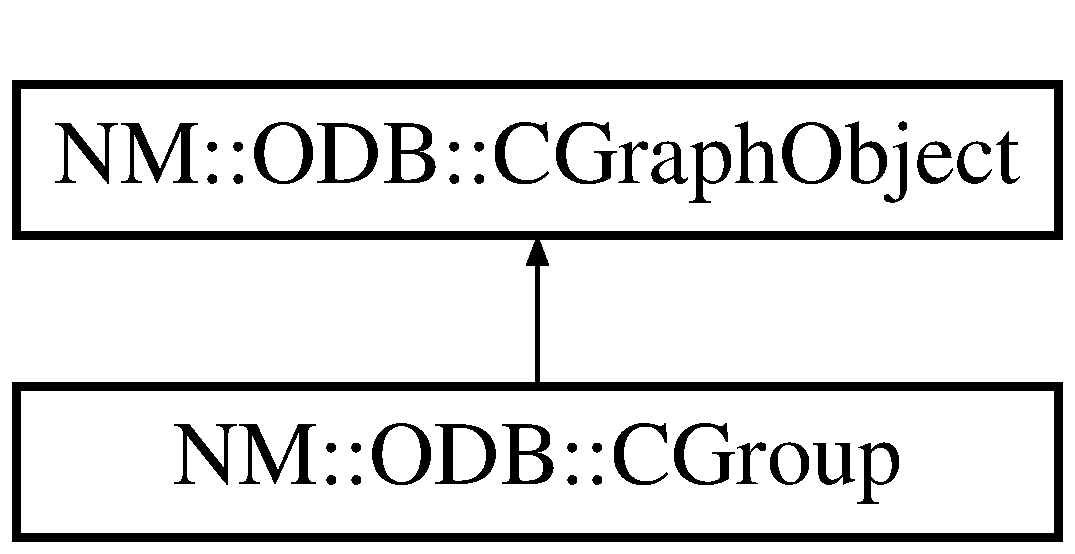
\includegraphics[height=2.000000cm]{class_n_m_1_1_o_d_b_1_1_c_group}
\end{center}
\end{figure}
\subsection*{Public Member Functions}
\begin{DoxyCompactItemize}
\item 
\hyperlink{class_n_m_1_1_o_d_b_1_1_c_group_aba1babf005f4718e0917ea77ce0e2cda}{C\+Group} ()
\item 
\hyperlink{class_n_m_1_1_o_d_b_1_1_c_group_a585eabaa9c717d45b28f7011173c218c}{$\sim$\+C\+Group} ()
\item 
\hyperlink{class_n_m_1_1_o_d_b_1_1_c_group}{C\+Group} $\ast$ \hyperlink{class_n_m_1_1_o_d_b_1_1_c_group_a3e5d4ed073cad6a4ceb06cab70c84c21}{clone} (size\+\_\+t new\+Object\+U\+I\+D) const 
\item 
\hyperlink{class_n_m_1_1_o_d_b_1_1_c_group_a651346a5c17274a9b886ccfee4cb178a}{C\+Group} (const \hyperlink{class_n_m_1_1_o_d_b_1_1_c_group}{C\+Group} \&o, const \hyperlink{namespace_n_m_1_1_o_d_b_a262b64fab56baaa96e18bac4ada88265}{O\+B\+J\+E\+C\+T\+U\+I\+D} New\+U\+I\+D)
\item 
bool \hyperlink{class_n_m_1_1_o_d_b_1_1_c_group_adff338636685a3b3562b86fd0d23bebb}{Point\+In\+Object} (int x, int y)
\end{DoxyCompactItemize}
\subsection*{Additional Inherited Members}


\subsection{Detailed Description}
Class \hyperlink{class_n_m_1_1_o_d_b_1_1_c_group}{C\+Group} 

\subsection{Constructor \& Destructor Documentation}
\hypertarget{class_n_m_1_1_o_d_b_1_1_c_group_aba1babf005f4718e0917ea77ce0e2cda}{}\index{N\+M\+::\+O\+D\+B\+::\+C\+Group@{N\+M\+::\+O\+D\+B\+::\+C\+Group}!C\+Group@{C\+Group}}
\index{C\+Group@{C\+Group}!N\+M\+::\+O\+D\+B\+::\+C\+Group@{N\+M\+::\+O\+D\+B\+::\+C\+Group}}
\subsubsection[{C\+Group()}]{\setlength{\rightskip}{0pt plus 5cm}N\+M\+::\+O\+D\+B\+::\+C\+Group\+::\+C\+Group (
\begin{DoxyParamCaption}
{}
\end{DoxyParamCaption}
)\hspace{0.3cm}{\ttfamily [inline]}}\label{class_n_m_1_1_o_d_b_1_1_c_group_aba1babf005f4718e0917ea77ce0e2cda}
\hypertarget{class_n_m_1_1_o_d_b_1_1_c_group_a585eabaa9c717d45b28f7011173c218c}{}\index{N\+M\+::\+O\+D\+B\+::\+C\+Group@{N\+M\+::\+O\+D\+B\+::\+C\+Group}!````~C\+Group@{$\sim$\+C\+Group}}
\index{````~C\+Group@{$\sim$\+C\+Group}!N\+M\+::\+O\+D\+B\+::\+C\+Group@{N\+M\+::\+O\+D\+B\+::\+C\+Group}}
\subsubsection[{$\sim$\+C\+Group()}]{\setlength{\rightskip}{0pt plus 5cm}N\+M\+::\+O\+D\+B\+::\+C\+Group\+::$\sim$\+C\+Group (
\begin{DoxyParamCaption}
{}
\end{DoxyParamCaption}
)\hspace{0.3cm}{\ttfamily [inline]}}\label{class_n_m_1_1_o_d_b_1_1_c_group_a585eabaa9c717d45b28f7011173c218c}
\hypertarget{class_n_m_1_1_o_d_b_1_1_c_group_a651346a5c17274a9b886ccfee4cb178a}{}\index{N\+M\+::\+O\+D\+B\+::\+C\+Group@{N\+M\+::\+O\+D\+B\+::\+C\+Group}!C\+Group@{C\+Group}}
\index{C\+Group@{C\+Group}!N\+M\+::\+O\+D\+B\+::\+C\+Group@{N\+M\+::\+O\+D\+B\+::\+C\+Group}}
\subsubsection[{C\+Group(const C\+Group \&o, const O\+B\+J\+E\+C\+T\+U\+I\+D New\+U\+I\+D)}]{\setlength{\rightskip}{0pt plus 5cm}N\+M\+::\+O\+D\+B\+::\+C\+Group\+::\+C\+Group (
\begin{DoxyParamCaption}
\item[{const {\bf C\+Group} \&}]{o, }
\item[{const {\bf O\+B\+J\+E\+C\+T\+U\+I\+D}}]{New\+U\+I\+D}
\end{DoxyParamCaption}
)\hspace{0.3cm}{\ttfamily [inline]}}\label{class_n_m_1_1_o_d_b_1_1_c_group_a651346a5c17274a9b886ccfee4cb178a}


\subsection{Member Function Documentation}
\hypertarget{class_n_m_1_1_o_d_b_1_1_c_group_a3e5d4ed073cad6a4ceb06cab70c84c21}{}\index{N\+M\+::\+O\+D\+B\+::\+C\+Group@{N\+M\+::\+O\+D\+B\+::\+C\+Group}!clone@{clone}}
\index{clone@{clone}!N\+M\+::\+O\+D\+B\+::\+C\+Group@{N\+M\+::\+O\+D\+B\+::\+C\+Group}}
\subsubsection[{clone(size\+\_\+t new\+Object\+U\+I\+D) const }]{\setlength{\rightskip}{0pt plus 5cm}{\bf C\+Group}$\ast$ N\+M\+::\+O\+D\+B\+::\+C\+Group\+::clone (
\begin{DoxyParamCaption}
\item[{size\+\_\+t}]{new\+Object\+U\+I\+D}
\end{DoxyParamCaption}
) const\hspace{0.3cm}{\ttfamily [inline]}, {\ttfamily [virtual]}}\label{class_n_m_1_1_o_d_b_1_1_c_group_a3e5d4ed073cad6a4ceb06cab70c84c21}


Implements \hyperlink{class_n_m_1_1_o_d_b_1_1_c_graph_object_aa0ca9ee294c6b42e39fb2c3a6598b506}{N\+M\+::\+O\+D\+B\+::\+C\+Graph\+Object}.

\hypertarget{class_n_m_1_1_o_d_b_1_1_c_group_adff338636685a3b3562b86fd0d23bebb}{}\index{N\+M\+::\+O\+D\+B\+::\+C\+Group@{N\+M\+::\+O\+D\+B\+::\+C\+Group}!Point\+In\+Object@{Point\+In\+Object}}
\index{Point\+In\+Object@{Point\+In\+Object}!N\+M\+::\+O\+D\+B\+::\+C\+Group@{N\+M\+::\+O\+D\+B\+::\+C\+Group}}
\subsubsection[{Point\+In\+Object(int x, int y)}]{\setlength{\rightskip}{0pt plus 5cm}bool N\+M\+::\+O\+D\+B\+::\+C\+Group\+::\+Point\+In\+Object (
\begin{DoxyParamCaption}
\item[{int}]{x, }
\item[{int}]{y}
\end{DoxyParamCaption}
)\hspace{0.3cm}{\ttfamily [inline]}}\label{class_n_m_1_1_o_d_b_1_1_c_group_adff338636685a3b3562b86fd0d23bebb}
void Draw\+Object(\+::\+Gdiplus\+::\+Graphics \&gr, \+::\+Gdiplus\+::\+Font \&font) \{ U\+N\+R\+E\+F\+E\+R\+E\+N\+C\+E\+D\+\_\+\+P\+A\+R\+A\+M\+E\+T\+E\+R(gr); U\+N\+R\+E\+F\+E\+R\+E\+N\+C\+E\+D\+\_\+\+P\+A\+R\+A\+M\+E\+T\+E\+R(font); \}; 

The documentation for this class was generated from the following file\+:\begin{DoxyCompactItemize}
\item 
C\+:/\+Users/\+Simon/\+Documents/\+Personal/\+Source Code/\+Projects/\+Network\+Modeller/\+Object\+Database/\+Data\+Objects/\hyperlink{_graph_objects_8h}{Graph\+Objects.\+h}\end{DoxyCompactItemize}

\hypertarget{class_n_m_1_1_o_d_b_1_1_c_layer}{}\section{N\+M\+:\+:O\+D\+B\+:\+:C\+Layer Class Reference}
\label{class_n_m_1_1_o_d_b_1_1_c_layer}\index{N\+M\+::\+O\+D\+B\+::\+C\+Layer@{N\+M\+::\+O\+D\+B\+::\+C\+Layer}}


{\ttfamily \#include $<$Graph\+Objects.\+h$>$}

Inheritance diagram for N\+M\+:\+:O\+D\+B\+:\+:C\+Layer\+:\begin{figure}[H]
\begin{center}
\leavevmode
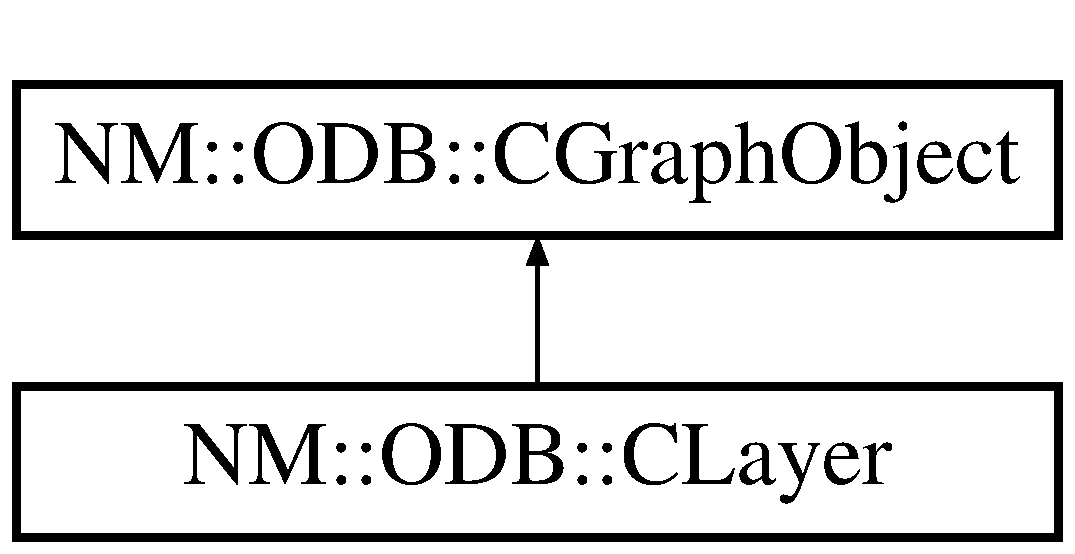
\includegraphics[height=2.000000cm]{class_n_m_1_1_o_d_b_1_1_c_layer}
\end{center}
\end{figure}
\subsection*{Public Member Functions}
\begin{DoxyCompactItemize}
\item 
\hyperlink{class_n_m_1_1_o_d_b_1_1_c_layer_a7da458775eac06098198c388edcff3d3}{C\+Layer} ()
\item 
\hyperlink{class_n_m_1_1_o_d_b_1_1_c_layer_a9f2abe118101e0f4eed653fc3d6230a1}{$\sim$\+C\+Layer} ()
\item 
\hyperlink{class_n_m_1_1_o_d_b_1_1_c_layer}{C\+Layer} $\ast$ \hyperlink{class_n_m_1_1_o_d_b_1_1_c_layer_a683492260348c94f9f3660f55d1a2438}{clone} (size\+\_\+t new\+Object\+U\+I\+D) const 
\item 
\hyperlink{class_n_m_1_1_o_d_b_1_1_c_layer_ac8dfe4da12a1fcb05517ff4567b5e3bb}{C\+Layer} (const \hyperlink{class_n_m_1_1_o_d_b_1_1_c_layer}{C\+Layer} \&o, const \hyperlink{namespace_n_m_1_1_o_d_b_a262b64fab56baaa96e18bac4ada88265}{O\+B\+J\+E\+C\+T\+U\+I\+D} New\+U\+I\+D)
\end{DoxyCompactItemize}
\subsection*{Friends}
\begin{DoxyCompactItemize}
\item 
class \hyperlink{class_n_m_1_1_o_d_b_1_1_c_layer_acc9f3446da3623694f17d73565a728db}{C\+Layer\+Table}
\end{DoxyCompactItemize}
\subsection*{Additional Inherited Members}


\subsection{Detailed Description}
Class \hyperlink{class_n_m_1_1_o_d_b_1_1_c_layer}{C\+Layer} 

\subsection{Constructor \& Destructor Documentation}
\hypertarget{class_n_m_1_1_o_d_b_1_1_c_layer_a7da458775eac06098198c388edcff3d3}{}\index{N\+M\+::\+O\+D\+B\+::\+C\+Layer@{N\+M\+::\+O\+D\+B\+::\+C\+Layer}!C\+Layer@{C\+Layer}}
\index{C\+Layer@{C\+Layer}!N\+M\+::\+O\+D\+B\+::\+C\+Layer@{N\+M\+::\+O\+D\+B\+::\+C\+Layer}}
\subsubsection[{C\+Layer()}]{\setlength{\rightskip}{0pt plus 5cm}N\+M\+::\+O\+D\+B\+::\+C\+Layer\+::\+C\+Layer (
\begin{DoxyParamCaption}
{}
\end{DoxyParamCaption}
)\hspace{0.3cm}{\ttfamily [inline]}}\label{class_n_m_1_1_o_d_b_1_1_c_layer_a7da458775eac06098198c388edcff3d3}
\hypertarget{class_n_m_1_1_o_d_b_1_1_c_layer_a9f2abe118101e0f4eed653fc3d6230a1}{}\index{N\+M\+::\+O\+D\+B\+::\+C\+Layer@{N\+M\+::\+O\+D\+B\+::\+C\+Layer}!````~C\+Layer@{$\sim$\+C\+Layer}}
\index{````~C\+Layer@{$\sim$\+C\+Layer}!N\+M\+::\+O\+D\+B\+::\+C\+Layer@{N\+M\+::\+O\+D\+B\+::\+C\+Layer}}
\subsubsection[{$\sim$\+C\+Layer()}]{\setlength{\rightskip}{0pt plus 5cm}N\+M\+::\+O\+D\+B\+::\+C\+Layer\+::$\sim$\+C\+Layer (
\begin{DoxyParamCaption}
{}
\end{DoxyParamCaption}
)\hspace{0.3cm}{\ttfamily [inline]}}\label{class_n_m_1_1_o_d_b_1_1_c_layer_a9f2abe118101e0f4eed653fc3d6230a1}
\hypertarget{class_n_m_1_1_o_d_b_1_1_c_layer_ac8dfe4da12a1fcb05517ff4567b5e3bb}{}\index{N\+M\+::\+O\+D\+B\+::\+C\+Layer@{N\+M\+::\+O\+D\+B\+::\+C\+Layer}!C\+Layer@{C\+Layer}}
\index{C\+Layer@{C\+Layer}!N\+M\+::\+O\+D\+B\+::\+C\+Layer@{N\+M\+::\+O\+D\+B\+::\+C\+Layer}}
\subsubsection[{C\+Layer(const C\+Layer \&o, const O\+B\+J\+E\+C\+T\+U\+I\+D New\+U\+I\+D)}]{\setlength{\rightskip}{0pt plus 5cm}N\+M\+::\+O\+D\+B\+::\+C\+Layer\+::\+C\+Layer (
\begin{DoxyParamCaption}
\item[{const {\bf C\+Layer} \&}]{o, }
\item[{const {\bf O\+B\+J\+E\+C\+T\+U\+I\+D}}]{New\+U\+I\+D}
\end{DoxyParamCaption}
)\hspace{0.3cm}{\ttfamily [inline]}}\label{class_n_m_1_1_o_d_b_1_1_c_layer_ac8dfe4da12a1fcb05517ff4567b5e3bb}


\subsection{Member Function Documentation}
\hypertarget{class_n_m_1_1_o_d_b_1_1_c_layer_a683492260348c94f9f3660f55d1a2438}{}\index{N\+M\+::\+O\+D\+B\+::\+C\+Layer@{N\+M\+::\+O\+D\+B\+::\+C\+Layer}!clone@{clone}}
\index{clone@{clone}!N\+M\+::\+O\+D\+B\+::\+C\+Layer@{N\+M\+::\+O\+D\+B\+::\+C\+Layer}}
\subsubsection[{clone(size\+\_\+t new\+Object\+U\+I\+D) const }]{\setlength{\rightskip}{0pt plus 5cm}{\bf C\+Layer}$\ast$ N\+M\+::\+O\+D\+B\+::\+C\+Layer\+::clone (
\begin{DoxyParamCaption}
\item[{size\+\_\+t}]{new\+Object\+U\+I\+D}
\end{DoxyParamCaption}
) const\hspace{0.3cm}{\ttfamily [inline]}, {\ttfamily [virtual]}}\label{class_n_m_1_1_o_d_b_1_1_c_layer_a683492260348c94f9f3660f55d1a2438}


Implements \hyperlink{class_n_m_1_1_o_d_b_1_1_c_graph_object_aa0ca9ee294c6b42e39fb2c3a6598b506}{N\+M\+::\+O\+D\+B\+::\+C\+Graph\+Object}.



\subsection{Friends And Related Function Documentation}
\hypertarget{class_n_m_1_1_o_d_b_1_1_c_layer_acc9f3446da3623694f17d73565a728db}{}\index{N\+M\+::\+O\+D\+B\+::\+C\+Layer@{N\+M\+::\+O\+D\+B\+::\+C\+Layer}!C\+Layer\+Table@{C\+Layer\+Table}}
\index{C\+Layer\+Table@{C\+Layer\+Table}!N\+M\+::\+O\+D\+B\+::\+C\+Layer@{N\+M\+::\+O\+D\+B\+::\+C\+Layer}}
\subsubsection[{C\+Layer\+Table}]{\setlength{\rightskip}{0pt plus 5cm}friend class {\bf C\+Layer\+Table}\hspace{0.3cm}{\ttfamily [friend]}}\label{class_n_m_1_1_o_d_b_1_1_c_layer_acc9f3446da3623694f17d73565a728db}


The documentation for this class was generated from the following file\+:\begin{DoxyCompactItemize}
\item 
C\+:/\+Users/\+Simon/\+Documents/\+Personal/\+Source Code/\+Projects/\+Network\+Modeller/\+Object\+Database/\+Data\+Objects/\hyperlink{_graph_objects_8h}{Graph\+Objects.\+h}\end{DoxyCompactItemize}

\hypertarget{class_n_m_1_1_o_d_b_1_1_c_layer_table}{}\section{N\+M\+:\+:O\+D\+B\+:\+:C\+Layer\+Table Class Reference}
\label{class_n_m_1_1_o_d_b_1_1_c_layer_table}\index{N\+M\+::\+O\+D\+B\+::\+C\+Layer\+Table@{N\+M\+::\+O\+D\+B\+::\+C\+Layer\+Table}}


{\ttfamily \#include $<$Layer\+Table.\+h$>$}

Inheritance diagram for N\+M\+:\+:O\+D\+B\+:\+:C\+Layer\+Table\+:\begin{figure}[H]
\begin{center}
\leavevmode
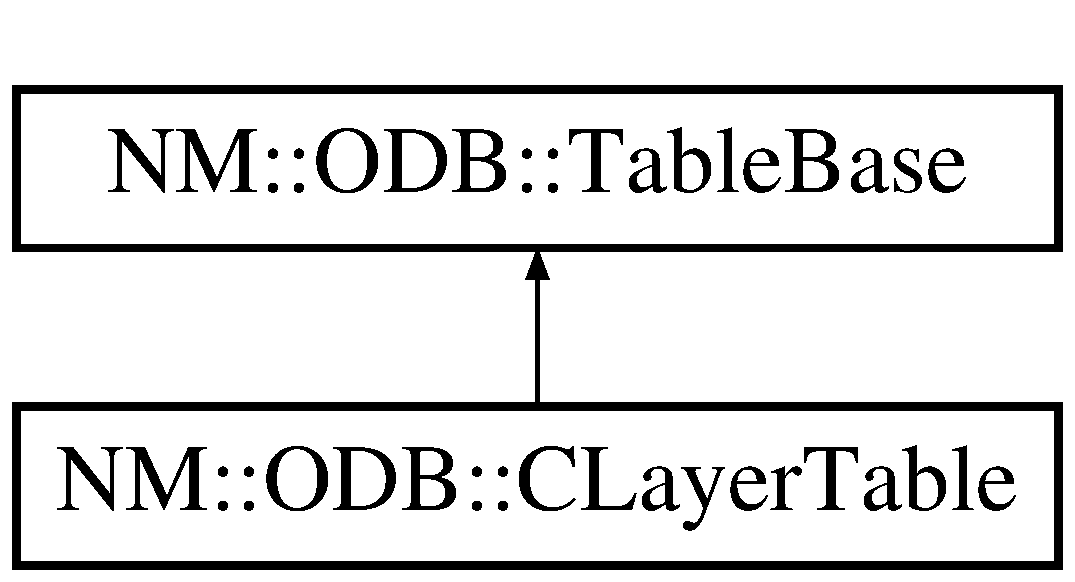
\includegraphics[height=2.000000cm]{class_n_m_1_1_o_d_b_1_1_c_layer_table}
\end{center}
\end{figure}
\subsection*{Public Types}
\begin{DoxyCompactItemize}
\item 
typedef \+::std\+::vector$<$ \hyperlink{class_n_m_1_1_o_d_b_1_1_c_layer}{C\+Layer} $\ast$ $>$\+::iterator \hyperlink{class_n_m_1_1_o_d_b_1_1_c_layer_table_a434102a84f3ecccf339809c0060fa80f}{L\+A\+Y\+E\+R\+\_\+\+I\+T\+E\+R\+A\+T\+O\+R}
\item 
typedef \+::std\+::vector$<$ \hyperlink{class_n_m_1_1_o_d_b_1_1_c_graph_object}{C\+Graph\+Object} $\ast$ $>$ \hyperlink{class_n_m_1_1_o_d_b_1_1_c_layer_table_ab1a405cd3c4cc2536d1af07fe96ddd92}{L\+A\+Y\+E\+R\+\_\+\+V\+E\+C\+T\+O\+R}
\end{DoxyCompactItemize}
\subsection*{Public Member Functions}
\begin{DoxyCompactItemize}
\item 
\hyperlink{class_n_m_1_1_o_d_b_1_1_c_layer_table_a3bd3aa3cfc0edd9188c6542484140a89}{C\+Layer\+Table} (\hyperlink{class_n_m_1_1_o_d_b_1_1_c_graph_object_factory}{C\+Graph\+Object\+Factory} $\ast$object\+Factory)
\item 
\hyperlink{class_n_m_1_1_o_d_b_1_1_c_layer_table_aee72d52f48bdc5d4ddc794c76c1860e0}{$\sim$\+C\+Layer\+Table} (void)
\item 
\hyperlink{namespace_n_m_1_1_o_d_b_a262b64fab56baaa96e18bac4ada88265}{O\+B\+J\+E\+C\+T\+U\+I\+D} \hyperlink{class_n_m_1_1_o_d_b_1_1_c_layer_table_a11754d097db8435c8e9320be09a2d067}{Create\+Layer} (\hyperlink{namespace_n_m_1_1_o_d_b_a8770283da9792324e1afe8104d40123b}{O\+B\+J\+E\+C\+T\+A\+T\+T\+R\+I\+B\+U\+T\+E\+S} $\ast$attribute\+Map I\+N, \hyperlink{class_n_m_1_1_o_d_b_1_1_c_graph_object}{C\+Graph\+Object} $\ast$$\ast$p\+Object O\+U\+T)
\item 
bool \hyperlink{class_n_m_1_1_o_d_b_1_1_c_layer_table_a1e39594b2ca8dae39543eb995f28a0c0}{Destroy\+Layer} (size\+\_\+t uid)
\item 
void \hyperlink{class_n_m_1_1_o_d_b_1_1_c_layer_table_aea55a9942f623ba6536f8c2bc6b976a8}{Clear} (void)
\item 
void \hyperlink{class_n_m_1_1_o_d_b_1_1_c_layer_table_aea0edc60fd8ad0e455c276c900a0b93c}{Refresh\+Layer\+Visibility} ()
\item 
\hyperlink{class_n_m_1_1_o_d_b_1_1_c_layer}{C\+Layer} $\ast$ \hyperlink{class_n_m_1_1_o_d_b_1_1_c_layer_table_ab733b17744ea9d457852662aabf7ed58}{Get\+Default\+Layer} ()
\item 
bool \hyperlink{class_n_m_1_1_o_d_b_1_1_c_layer_table_a71a6bb2dbac48f3dd636c25d7d1b31f0}{Set\+Value} (\hyperlink{class_n_m_1_1_o_d_b_1_1_c_graph_object}{C\+Graph\+Object} $\ast$, size\+\_\+t idx, \hyperlink{class_n_m_1_1_o_d_b_1_1_value}{Value} const \&v)
\item 
bool \hyperlink{class_n_m_1_1_o_d_b_1_1_c_layer_table_a589923308ca7e92665b9999572d36bbd}{Set\+Value} (\hyperlink{class_n_m_1_1_o_d_b_1_1_c_graph_object}{C\+Graph\+Object} $\ast$, const \+::std\+::wstring \&attrname, \hyperlink{class_n_m_1_1_o_d_b_1_1_value}{Value} const \&v)
\end{DoxyCompactItemize}
\subsection*{Public Attributes}
\begin{DoxyCompactItemize}
\item 
\hyperlink{class_n_m_1_1_o_d_b_1_1_c_layer_table_ab1a405cd3c4cc2536d1af07fe96ddd92}{L\+A\+Y\+E\+R\+\_\+\+V\+E\+C\+T\+O\+R} \hyperlink{class_n_m_1_1_o_d_b_1_1_c_layer_table_a24f25cc4cd1e097b5c66f25369654fed}{layers}
\end{DoxyCompactItemize}
\subsection*{Friends}
\begin{DoxyCompactItemize}
\item 
class \hyperlink{class_n_m_1_1_o_d_b_1_1_c_layer_table_a8451ee9e81bc51a04afb10dc6ee7e07e}{C\+Object\+Database}
\end{DoxyCompactItemize}


\subsection{Member Typedef Documentation}
\hypertarget{class_n_m_1_1_o_d_b_1_1_c_layer_table_a434102a84f3ecccf339809c0060fa80f}{}\index{N\+M\+::\+O\+D\+B\+::\+C\+Layer\+Table@{N\+M\+::\+O\+D\+B\+::\+C\+Layer\+Table}!L\+A\+Y\+E\+R\+\_\+\+I\+T\+E\+R\+A\+T\+O\+R@{L\+A\+Y\+E\+R\+\_\+\+I\+T\+E\+R\+A\+T\+O\+R}}
\index{L\+A\+Y\+E\+R\+\_\+\+I\+T\+E\+R\+A\+T\+O\+R@{L\+A\+Y\+E\+R\+\_\+\+I\+T\+E\+R\+A\+T\+O\+R}!N\+M\+::\+O\+D\+B\+::\+C\+Layer\+Table@{N\+M\+::\+O\+D\+B\+::\+C\+Layer\+Table}}
\subsubsection[{L\+A\+Y\+E\+R\+\_\+\+I\+T\+E\+R\+A\+T\+O\+R}]{\setlength{\rightskip}{0pt plus 5cm}typedef \+::std\+::vector$<${\bf C\+Layer}$\ast$$>$\+::iterator {\bf N\+M\+::\+O\+D\+B\+::\+C\+Layer\+Table\+::\+L\+A\+Y\+E\+R\+\_\+\+I\+T\+E\+R\+A\+T\+O\+R}}\label{class_n_m_1_1_o_d_b_1_1_c_layer_table_a434102a84f3ecccf339809c0060fa80f}
\hypertarget{class_n_m_1_1_o_d_b_1_1_c_layer_table_ab1a405cd3c4cc2536d1af07fe96ddd92}{}\index{N\+M\+::\+O\+D\+B\+::\+C\+Layer\+Table@{N\+M\+::\+O\+D\+B\+::\+C\+Layer\+Table}!L\+A\+Y\+E\+R\+\_\+\+V\+E\+C\+T\+O\+R@{L\+A\+Y\+E\+R\+\_\+\+V\+E\+C\+T\+O\+R}}
\index{L\+A\+Y\+E\+R\+\_\+\+V\+E\+C\+T\+O\+R@{L\+A\+Y\+E\+R\+\_\+\+V\+E\+C\+T\+O\+R}!N\+M\+::\+O\+D\+B\+::\+C\+Layer\+Table@{N\+M\+::\+O\+D\+B\+::\+C\+Layer\+Table}}
\subsubsection[{L\+A\+Y\+E\+R\+\_\+\+V\+E\+C\+T\+O\+R}]{\setlength{\rightskip}{0pt plus 5cm}typedef \+::std\+::vector$<${\bf C\+Graph\+Object}$\ast$$>$ {\bf N\+M\+::\+O\+D\+B\+::\+C\+Layer\+Table\+::\+L\+A\+Y\+E\+R\+\_\+\+V\+E\+C\+T\+O\+R}}\label{class_n_m_1_1_o_d_b_1_1_c_layer_table_ab1a405cd3c4cc2536d1af07fe96ddd92}


\subsection{Constructor \& Destructor Documentation}
\hypertarget{class_n_m_1_1_o_d_b_1_1_c_layer_table_a3bd3aa3cfc0edd9188c6542484140a89}{}\index{N\+M\+::\+O\+D\+B\+::\+C\+Layer\+Table@{N\+M\+::\+O\+D\+B\+::\+C\+Layer\+Table}!C\+Layer\+Table@{C\+Layer\+Table}}
\index{C\+Layer\+Table@{C\+Layer\+Table}!N\+M\+::\+O\+D\+B\+::\+C\+Layer\+Table@{N\+M\+::\+O\+D\+B\+::\+C\+Layer\+Table}}
\subsubsection[{C\+Layer\+Table(\+C\+Graph\+Object\+Factory $\ast$object\+Factory)}]{\setlength{\rightskip}{0pt plus 5cm}N\+M\+::\+O\+D\+B\+::\+C\+Layer\+Table\+::\+C\+Layer\+Table (
\begin{DoxyParamCaption}
\item[{{\bf C\+Graph\+Object\+Factory} $\ast$}]{object\+Factory}
\end{DoxyParamCaption}
)}\label{class_n_m_1_1_o_d_b_1_1_c_layer_table_a3bd3aa3cfc0edd9188c6542484140a89}
\hypertarget{class_n_m_1_1_o_d_b_1_1_c_layer_table_aee72d52f48bdc5d4ddc794c76c1860e0}{}\index{N\+M\+::\+O\+D\+B\+::\+C\+Layer\+Table@{N\+M\+::\+O\+D\+B\+::\+C\+Layer\+Table}!````~C\+Layer\+Table@{$\sim$\+C\+Layer\+Table}}
\index{````~C\+Layer\+Table@{$\sim$\+C\+Layer\+Table}!N\+M\+::\+O\+D\+B\+::\+C\+Layer\+Table@{N\+M\+::\+O\+D\+B\+::\+C\+Layer\+Table}}
\subsubsection[{$\sim$\+C\+Layer\+Table(void)}]{\setlength{\rightskip}{0pt plus 5cm}N\+M\+::\+O\+D\+B\+::\+C\+Layer\+Table\+::$\sim$\+C\+Layer\+Table (
\begin{DoxyParamCaption}
\item[{void}]{}
\end{DoxyParamCaption}
)}\label{class_n_m_1_1_o_d_b_1_1_c_layer_table_aee72d52f48bdc5d4ddc794c76c1860e0}


\subsection{Member Function Documentation}
\hypertarget{class_n_m_1_1_o_d_b_1_1_c_layer_table_aea55a9942f623ba6536f8c2bc6b976a8}{}\index{N\+M\+::\+O\+D\+B\+::\+C\+Layer\+Table@{N\+M\+::\+O\+D\+B\+::\+C\+Layer\+Table}!Clear@{Clear}}
\index{Clear@{Clear}!N\+M\+::\+O\+D\+B\+::\+C\+Layer\+Table@{N\+M\+::\+O\+D\+B\+::\+C\+Layer\+Table}}
\subsubsection[{Clear(void)}]{\setlength{\rightskip}{0pt plus 5cm}void N\+M\+::\+O\+D\+B\+::\+C\+Layer\+Table\+::\+Clear (
\begin{DoxyParamCaption}
\item[{void}]{}
\end{DoxyParamCaption}
)}\label{class_n_m_1_1_o_d_b_1_1_c_layer_table_aea55a9942f623ba6536f8c2bc6b976a8}
\hypertarget{class_n_m_1_1_o_d_b_1_1_c_layer_table_a11754d097db8435c8e9320be09a2d067}{}\index{N\+M\+::\+O\+D\+B\+::\+C\+Layer\+Table@{N\+M\+::\+O\+D\+B\+::\+C\+Layer\+Table}!Create\+Layer@{Create\+Layer}}
\index{Create\+Layer@{Create\+Layer}!N\+M\+::\+O\+D\+B\+::\+C\+Layer\+Table@{N\+M\+::\+O\+D\+B\+::\+C\+Layer\+Table}}
\subsubsection[{Create\+Layer(\+O\+B\+J\+E\+C\+T\+A\+T\+T\+R\+I\+B\+U\+T\+E\+S $\ast$attribute\+Map I\+N, C\+Graph\+Object $\ast$$\ast$p\+Object O\+U\+T)}]{\setlength{\rightskip}{0pt plus 5cm}{\bf O\+B\+J\+E\+C\+T\+U\+I\+D} N\+M\+::\+O\+D\+B\+::\+C\+Layer\+Table\+::\+Create\+Layer (
\begin{DoxyParamCaption}
\item[{{\bf O\+B\+J\+E\+C\+T\+A\+T\+T\+R\+I\+B\+U\+T\+E\+S} $\ast$attribute\+Map}]{I\+N, }
\item[{{\bf C\+Graph\+Object} $\ast$$\ast$p\+Object}]{O\+U\+T}
\end{DoxyParamCaption}
)}\label{class_n_m_1_1_o_d_b_1_1_c_layer_table_a11754d097db8435c8e9320be09a2d067}
\hypertarget{class_n_m_1_1_o_d_b_1_1_c_layer_table_a1e39594b2ca8dae39543eb995f28a0c0}{}\index{N\+M\+::\+O\+D\+B\+::\+C\+Layer\+Table@{N\+M\+::\+O\+D\+B\+::\+C\+Layer\+Table}!Destroy\+Layer@{Destroy\+Layer}}
\index{Destroy\+Layer@{Destroy\+Layer}!N\+M\+::\+O\+D\+B\+::\+C\+Layer\+Table@{N\+M\+::\+O\+D\+B\+::\+C\+Layer\+Table}}
\subsubsection[{Destroy\+Layer(size\+\_\+t uid)}]{\setlength{\rightskip}{0pt plus 5cm}bool N\+M\+::\+O\+D\+B\+::\+C\+Layer\+Table\+::\+Destroy\+Layer (
\begin{DoxyParamCaption}
\item[{size\+\_\+t}]{uid}
\end{DoxyParamCaption}
)}\label{class_n_m_1_1_o_d_b_1_1_c_layer_table_a1e39594b2ca8dae39543eb995f28a0c0}
\hypertarget{class_n_m_1_1_o_d_b_1_1_c_layer_table_ab733b17744ea9d457852662aabf7ed58}{}\index{N\+M\+::\+O\+D\+B\+::\+C\+Layer\+Table@{N\+M\+::\+O\+D\+B\+::\+C\+Layer\+Table}!Get\+Default\+Layer@{Get\+Default\+Layer}}
\index{Get\+Default\+Layer@{Get\+Default\+Layer}!N\+M\+::\+O\+D\+B\+::\+C\+Layer\+Table@{N\+M\+::\+O\+D\+B\+::\+C\+Layer\+Table}}
\subsubsection[{Get\+Default\+Layer()}]{\setlength{\rightskip}{0pt plus 5cm}{\bf C\+Layer}$\ast$ N\+M\+::\+O\+D\+B\+::\+C\+Layer\+Table\+::\+Get\+Default\+Layer (
\begin{DoxyParamCaption}
{}
\end{DoxyParamCaption}
)}\label{class_n_m_1_1_o_d_b_1_1_c_layer_table_ab733b17744ea9d457852662aabf7ed58}
\hypertarget{class_n_m_1_1_o_d_b_1_1_c_layer_table_aea0edc60fd8ad0e455c276c900a0b93c}{}\index{N\+M\+::\+O\+D\+B\+::\+C\+Layer\+Table@{N\+M\+::\+O\+D\+B\+::\+C\+Layer\+Table}!Refresh\+Layer\+Visibility@{Refresh\+Layer\+Visibility}}
\index{Refresh\+Layer\+Visibility@{Refresh\+Layer\+Visibility}!N\+M\+::\+O\+D\+B\+::\+C\+Layer\+Table@{N\+M\+::\+O\+D\+B\+::\+C\+Layer\+Table}}
\subsubsection[{Refresh\+Layer\+Visibility()}]{\setlength{\rightskip}{0pt plus 5cm}void N\+M\+::\+O\+D\+B\+::\+C\+Layer\+Table\+::\+Refresh\+Layer\+Visibility (
\begin{DoxyParamCaption}
{}
\end{DoxyParamCaption}
)}\label{class_n_m_1_1_o_d_b_1_1_c_layer_table_aea0edc60fd8ad0e455c276c900a0b93c}
\hypertarget{class_n_m_1_1_o_d_b_1_1_c_layer_table_a71a6bb2dbac48f3dd636c25d7d1b31f0}{}\index{N\+M\+::\+O\+D\+B\+::\+C\+Layer\+Table@{N\+M\+::\+O\+D\+B\+::\+C\+Layer\+Table}!Set\+Value@{Set\+Value}}
\index{Set\+Value@{Set\+Value}!N\+M\+::\+O\+D\+B\+::\+C\+Layer\+Table@{N\+M\+::\+O\+D\+B\+::\+C\+Layer\+Table}}
\subsubsection[{Set\+Value(\+C\+Graph\+Object $\ast$, size\+\_\+t idx, Value const \&v)}]{\setlength{\rightskip}{0pt plus 5cm}bool N\+M\+::\+O\+D\+B\+::\+C\+Layer\+Table\+::\+Set\+Value (
\begin{DoxyParamCaption}
\item[{{\bf C\+Graph\+Object} $\ast$}]{layer, }
\item[{size\+\_\+t}]{idx, }
\item[{{\bf Value} const \&}]{v}
\end{DoxyParamCaption}
)\hspace{0.3cm}{\ttfamily [virtual]}}\label{class_n_m_1_1_o_d_b_1_1_c_layer_table_a71a6bb2dbac48f3dd636c25d7d1b31f0}


Implements \hyperlink{class_n_m_1_1_o_d_b_1_1_table_base_afbc340c36e140f2a8184d2585cc3b5d5}{N\+M\+::\+O\+D\+B\+::\+Table\+Base}.

\hypertarget{class_n_m_1_1_o_d_b_1_1_c_layer_table_a589923308ca7e92665b9999572d36bbd}{}\index{N\+M\+::\+O\+D\+B\+::\+C\+Layer\+Table@{N\+M\+::\+O\+D\+B\+::\+C\+Layer\+Table}!Set\+Value@{Set\+Value}}
\index{Set\+Value@{Set\+Value}!N\+M\+::\+O\+D\+B\+::\+C\+Layer\+Table@{N\+M\+::\+O\+D\+B\+::\+C\+Layer\+Table}}
\subsubsection[{Set\+Value(\+C\+Graph\+Object $\ast$, const \+::std\+::wstring \&attrname, Value const \&v)}]{\setlength{\rightskip}{0pt plus 5cm}bool N\+M\+::\+O\+D\+B\+::\+C\+Layer\+Table\+::\+Set\+Value (
\begin{DoxyParamCaption}
\item[{{\bf C\+Graph\+Object} $\ast$}]{layer, }
\item[{const \+::std\+::wstring \&}]{attrname, }
\item[{{\bf Value} const \&}]{v}
\end{DoxyParamCaption}
)\hspace{0.3cm}{\ttfamily [virtual]}}\label{class_n_m_1_1_o_d_b_1_1_c_layer_table_a589923308ca7e92665b9999572d36bbd}


Implements \hyperlink{class_n_m_1_1_o_d_b_1_1_table_base_a3e55bfe64ccdf81e6a96941b3f9a5fb4}{N\+M\+::\+O\+D\+B\+::\+Table\+Base}.



\subsection{Friends And Related Function Documentation}
\hypertarget{class_n_m_1_1_o_d_b_1_1_c_layer_table_a8451ee9e81bc51a04afb10dc6ee7e07e}{}\index{N\+M\+::\+O\+D\+B\+::\+C\+Layer\+Table@{N\+M\+::\+O\+D\+B\+::\+C\+Layer\+Table}!C\+Object\+Database@{C\+Object\+Database}}
\index{C\+Object\+Database@{C\+Object\+Database}!N\+M\+::\+O\+D\+B\+::\+C\+Layer\+Table@{N\+M\+::\+O\+D\+B\+::\+C\+Layer\+Table}}
\subsubsection[{C\+Object\+Database}]{\setlength{\rightskip}{0pt plus 5cm}friend class {\bf C\+Object\+Database}\hspace{0.3cm}{\ttfamily [friend]}}\label{class_n_m_1_1_o_d_b_1_1_c_layer_table_a8451ee9e81bc51a04afb10dc6ee7e07e}


\subsection{Member Data Documentation}
\hypertarget{class_n_m_1_1_o_d_b_1_1_c_layer_table_a24f25cc4cd1e097b5c66f25369654fed}{}\index{N\+M\+::\+O\+D\+B\+::\+C\+Layer\+Table@{N\+M\+::\+O\+D\+B\+::\+C\+Layer\+Table}!layers@{layers}}
\index{layers@{layers}!N\+M\+::\+O\+D\+B\+::\+C\+Layer\+Table@{N\+M\+::\+O\+D\+B\+::\+C\+Layer\+Table}}
\subsubsection[{layers}]{\setlength{\rightskip}{0pt plus 5cm}{\bf L\+A\+Y\+E\+R\+\_\+\+V\+E\+C\+T\+O\+R} N\+M\+::\+O\+D\+B\+::\+C\+Layer\+Table\+::layers}\label{class_n_m_1_1_o_d_b_1_1_c_layer_table_a24f25cc4cd1e097b5c66f25369654fed}


The documentation for this class was generated from the following files\+:\begin{DoxyCompactItemize}
\item 
C\+:/\+Users/\+Simon/\+Documents/\+Personal/\+Source Code/\+Projects/\+Network\+Modeller/\+Object\+Database/\+Tables/\hyperlink{_layer_table_8h}{Layer\+Table.\+h}\item 
C\+:/\+Users/\+Simon/\+Documents/\+Personal/\+Source Code/\+Projects/\+Network\+Modeller/\+Object\+Database/\+Tables/\hyperlink{_layer_table_8cpp}{Layer\+Table.\+cpp}\end{DoxyCompactItemize}

\hypertarget{class_n_m_1_1_o_d_b_1_1_c_object_database}{}\section{N\+M\+:\+:O\+D\+B\+:\+:C\+Object\+Database Class Reference}
\label{class_n_m_1_1_o_d_b_1_1_c_object_database}\index{N\+M\+::\+O\+D\+B\+::\+C\+Object\+Database@{N\+M\+::\+O\+D\+B\+::\+C\+Object\+Database}}


{\ttfamily \#include $<$Object\+Database.\+h$>$}

Inheritance diagram for N\+M\+:\+:O\+D\+B\+:\+:C\+Object\+Database\+:\begin{figure}[H]
\begin{center}
\leavevmode
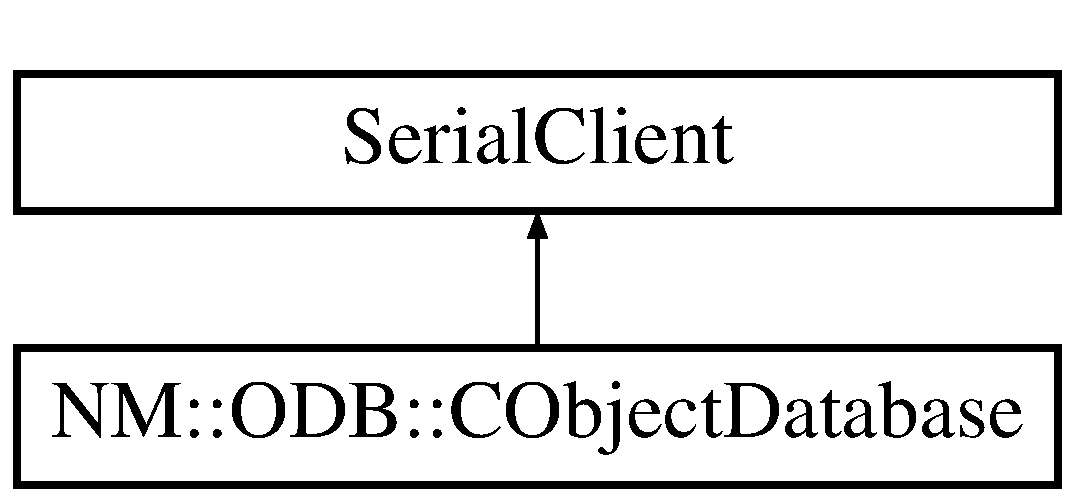
\includegraphics[height=2.000000cm]{class_n_m_1_1_o_d_b_1_1_c_object_database}
\end{center}
\end{figure}
\subsection*{Public Types}
\begin{DoxyCompactItemize}
\item 
enum \hyperlink{class_n_m_1_1_o_d_b_1_1_c_object_database_a706b0a517469d7c4ddf2a8a7730219de}{N\+O\+T\+I\+F\+Y\+\_\+\+T\+Y\+P\+E} \{ \hyperlink{class_n_m_1_1_o_d_b_1_1_c_object_database_a706b0a517469d7c4ddf2a8a7730219dead32c7592a66e6e96f15b43c9d9f13846}{N\+O\+T\+I\+F\+Y\+\_\+\+T\+Y\+P\+E\+::\+N\+O\+T\+I\+F\+Y\+\_\+\+A\+D\+D} = 1, 
\hyperlink{class_n_m_1_1_o_d_b_1_1_c_object_database_a706b0a517469d7c4ddf2a8a7730219dea3d2b0ba9bc47406c9c5abeccfcdba46e}{N\+O\+T\+I\+F\+Y\+\_\+\+T\+Y\+P\+E\+::\+N\+O\+T\+I\+F\+Y\+\_\+\+D\+E\+L\+E\+T\+E} = 2, 
\hyperlink{class_n_m_1_1_o_d_b_1_1_c_object_database_a706b0a517469d7c4ddf2a8a7730219deaa9649df4997d00fcfd6e3747944bcff7}{N\+O\+T\+I\+F\+Y\+\_\+\+T\+Y\+P\+E\+::\+N\+O\+T\+I\+F\+Y\+\_\+\+C\+H\+A\+N\+G\+E} = 4
 \}
\item 
typedef \+::std\+::vector$<$\+::std\+::wstring $>$ \hyperlink{class_n_m_1_1_o_d_b_1_1_c_object_database_af71c35cd26a6e83732da7ae538c665a0}{Object\+Attribute\+List}
\end{DoxyCompactItemize}
\subsection*{Public Member Functions}
\begin{DoxyCompactItemize}
\item 
\hyperlink{class_n_m_1_1_o_d_b_1_1_c_object_database_ac22aeb28f89fdc575ff17e23196d13ad}{$\sim$\+C\+Object\+Database} ()
\item 
bool \hyperlink{class_n_m_1_1_o_d_b_1_1_c_object_database_aa5efd0c00741e844d60ac6d24bb501c5}{Register\+Observer} (\hyperlink{class_n_m_1_1_o_d_b_1_1_c_database_observer}{C\+Database\+Observer} $\ast$p\+Observer,\+::std\+::wstring \&obsname, \hyperlink{namespace_n_m_1_1_o_d_b_ac9f60beb4a1c8a6240dd0c8baa281345}{Object\+Type},\+::std\+::vector$<$\+::std\+::wstring $>$ \&attribute\+\_\+list)
\item 
void \hyperlink{class_n_m_1_1_o_d_b_1_1_c_object_database_a8213fa91ed5c5dc93d68399729e70d59}{Un\+Register\+Observer} (\hyperlink{class_n_m_1_1_o_d_b_1_1_c_database_observer}{C\+Database\+Observer} $\ast$p\+Observer)
\item 
\hyperlink{namespace_n_m_1_1_o_d_b_a262b64fab56baaa96e18bac4ada88265}{O\+B\+J\+E\+C\+T\+U\+I\+D} \hyperlink{class_n_m_1_1_o_d_b_1_1_c_object_database_a6dbe5739671f32073170e57601ff7ad6}{Create\+Vertex} (\hyperlink{namespace_n_m_1_1_o_d_b_a74e0c94daaeea6f7e783c03a8c921022}{Vertex\+Type} vertex\+Type, \hyperlink{namespace_n_m_1_1_o_d_b_a8770283da9792324e1afe8104d40123b}{O\+B\+J\+E\+C\+T\+A\+T\+T\+R\+I\+B\+U\+T\+E\+S} $\ast$attribute\+Map)
\item 
\hyperlink{namespace_n_m_1_1_o_d_b_a262b64fab56baaa96e18bac4ada88265}{O\+B\+J\+E\+C\+T\+U\+I\+D} \hyperlink{class_n_m_1_1_o_d_b_1_1_c_object_database_af00951e6e3d9368b223ce4a68da60afb}{Create\+Edge} (\hyperlink{namespace_n_m_1_1_o_d_b_a8770283da9792324e1afe8104d40123b}{O\+B\+J\+E\+C\+T\+A\+T\+T\+R\+I\+B\+U\+T\+E\+S} $\ast$attribute\+Map)
\item 
\hyperlink{namespace_n_m_1_1_o_d_b_a262b64fab56baaa96e18bac4ada88265}{O\+B\+J\+E\+C\+T\+U\+I\+D} \hyperlink{class_n_m_1_1_o_d_b_1_1_c_object_database_ae861a71ba9030e0abd909f751aae1bdf}{Create\+Layer} (\hyperlink{namespace_n_m_1_1_o_d_b_a8770283da9792324e1afe8104d40123b}{O\+B\+J\+E\+C\+T\+A\+T\+T\+R\+I\+B\+U\+T\+E\+S} $\ast$attribute\+Map)
\item 
\hyperlink{namespace_n_m_1_1_o_d_b_a262b64fab56baaa96e18bac4ada88265}{O\+B\+J\+E\+C\+T\+U\+I\+D} \hyperlink{class_n_m_1_1_o_d_b_1_1_c_object_database_a693e0861663bbc1f73f3477ba43bcdc1}{Copy\+Vertex} (\hyperlink{namespace_n_m_1_1_o_d_b_a262b64fab56baaa96e18bac4ada88265}{O\+B\+J\+E\+C\+T\+U\+I\+D} source\+Object\+U\+I\+D)
\item 
void \hyperlink{class_n_m_1_1_o_d_b_1_1_c_object_database_a9920f00990810478e38480dee826ec5e}{Delete\+Object} (\hyperlink{namespace_n_m_1_1_o_d_b_a262b64fab56baaa96e18bac4ada88265}{O\+B\+J\+E\+C\+T\+U\+I\+D} object\+U\+I\+D, bool notify)
\item 
\hyperlink{namespace_n_m_1_1_o_d_b_ac9f60beb4a1c8a6240dd0c8baa281345}{Object\+Type} \hyperlink{class_n_m_1_1_o_d_b_1_1_c_object_database_a11952794073e4f0e0ea80561b6a7d451}{Get\+Object\+Type} (\hyperlink{namespace_n_m_1_1_o_d_b_a262b64fab56baaa96e18bac4ada88265}{O\+B\+J\+E\+C\+T\+U\+I\+D} object\+U\+I\+D)
\item 
bool \hyperlink{class_n_m_1_1_o_d_b_1_1_c_object_database_ab493c329da6a01087731de252dfcb7cb}{Validate\+Object\+U\+I\+D} (\hyperlink{namespace_n_m_1_1_o_d_b_a8770283da9792324e1afe8104d40123b}{O\+B\+J\+E\+C\+T\+A\+T\+T\+R\+I\+B\+U\+T\+E\+S} $\ast$attribute\+Map)
\item 
bool \hyperlink{class_n_m_1_1_o_d_b_1_1_c_object_database_a2576cb7591c07b7bafde7a202c893d83}{Set\+Value} (\hyperlink{namespace_n_m_1_1_o_d_b_a262b64fab56baaa96e18bac4ada88265}{O\+B\+J\+E\+C\+T\+U\+I\+D} objectuid, size\+\_\+t attribute\+Index, \hyperlink{class_n_m_1_1_o_d_b_1_1_value}{Value} const \&v)
\item 
bool \hyperlink{class_n_m_1_1_o_d_b_1_1_c_object_database_abad2ed76b834f69fa8ec4c3dcadd9630}{Set\+Value} (\hyperlink{namespace_n_m_1_1_o_d_b_a262b64fab56baaa96e18bac4ada88265}{O\+B\+J\+E\+C\+T\+U\+I\+D} objectuid, const \+::std\+::wstring \&attrname, \hyperlink{class_n_m_1_1_o_d_b_1_1_value}{Value} const \&v)
\item 
\hyperlink{namespace_n_m_1_1_o_d_b_a76ab348a70a5cf877035b8281bdd3f7b}{S\+P\+V\+A\+L\+U\+E} \hyperlink{class_n_m_1_1_o_d_b_1_1_c_object_database_a2683920d3ec18c355adb9bf9168ae9a4}{Get\+Value} (\hyperlink{namespace_n_m_1_1_o_d_b_a262b64fab56baaa96e18bac4ada88265}{O\+B\+J\+E\+C\+T\+U\+I\+D} objectuid, size\+\_\+t attribute\+Index) const 
\item 
\hyperlink{namespace_n_m_1_1_o_d_b_a76ab348a70a5cf877035b8281bdd3f7b}{S\+P\+V\+A\+L\+U\+E} \hyperlink{class_n_m_1_1_o_d_b_1_1_c_object_database_a25d14d82a6cd4f59bf2ce0a4cbcce0e6}{Get\+Value} (\hyperlink{namespace_n_m_1_1_o_d_b_a262b64fab56baaa96e18bac4ada88265}{O\+B\+J\+E\+C\+T\+U\+I\+D} objectuid, const \+::std\+::wstring \&attrname)
\item 
\hyperlink{namespace_n_m_1_1_o_d_b_a262b64fab56baaa96e18bac4ada88265}{O\+B\+J\+E\+C\+T\+U\+I\+D} \hyperlink{class_n_m_1_1_o_d_b_1_1_c_object_database_a6e76fad89f4de84dbdda126601efc837}{Get\+Vertex\+Sibling} (\hyperlink{namespace_n_m_1_1_o_d_b_a74e0c94daaeea6f7e783c03a8c921022}{Vertex\+Type} v\+Type, \hyperlink{namespace_n_m_1_1_o_d_b_a1b474aa7e937112cda42381969dcb55e}{Sibling\+Position} position)
\item 
\hyperlink{namespace_n_m_1_1_o_d_b_a262b64fab56baaa96e18bac4ada88265}{O\+B\+J\+E\+C\+T\+U\+I\+D} \hyperlink{class_n_m_1_1_o_d_b_1_1_c_object_database_a133d5a5d74bacdeba535fa55a2bd45ff}{Get\+Edge\+Sibling} (\hyperlink{namespace_n_m_1_1_o_d_b_a1ac3948936d4d0ab4367d35aa46068da}{Edge\+Type} e\+Type, \hyperlink{namespace_n_m_1_1_o_d_b_a1b474aa7e937112cda42381969dcb55e}{Sibling\+Position} position)
\item 
bool \hyperlink{class_n_m_1_1_o_d_b_1_1_c_object_database_a513e5758995acc1122abe83b1af6a9cf}{Load\+X\+M\+L\+Data} (tinyxml2\+::\+X\+M\+L\+Document $\ast$dest\+Doc, tinyxml2\+::\+X\+M\+L\+Node $\ast$current\+Node)
\item 
bool \hyperlink{class_n_m_1_1_o_d_b_1_1_c_object_database_a596806ff34088c667d0a161c4ddae14b}{Save\+X\+M\+L\+Data} (tinyxml2\+::\+X\+M\+L\+Document $\ast$dest\+Doc, tinyxml2\+::\+X\+M\+L\+Node $\ast$current\+Node)
\item 
void \hyperlink{class_n_m_1_1_o_d_b_1_1_c_object_database_afc48afb9b5beaa4797e0ab8d18b23f8b}{Clear} ()
\item 
unsigned int \hyperlink{class_n_m_1_1_o_d_b_1_1_c_object_database_ad0aaec454e7e12357f935b410503e60a}{Begin\+Update} ()
\item 
unsigned int \hyperlink{class_n_m_1_1_o_d_b_1_1_c_object_database_abbe4d83bfe24587f8bb2106d714dc2bc}{End\+Update} ()
\item 
\hyperlink{class_n_m_1_1_o_d_b_1_1_i_adjacency_matrix}{I\+Adjacency\+Matrix} \hyperlink{class_n_m_1_1_o_d_b_1_1_c_object_database_a5070b38870a434bac91e9b0445be7667}{Get\+Adjacency\+Matrix} ()
\item 
size\+\_\+t \hyperlink{class_n_m_1_1_o_d_b_1_1_c_object_database_ab7d8f69610a340eef06f979773ca2452}{Get\+Vertex\+Count} ()
\item 
size\+\_\+t \hyperlink{class_n_m_1_1_o_d_b_1_1_c_object_database_adaaa910be8b729b5fc6d23131c5e9dbd}{Get\+Edge\+Count} ()
\item 
size\+\_\+t \hyperlink{class_n_m_1_1_o_d_b_1_1_c_object_database_a02e7243f308498936443a6e34bece14e}{Get\+Vertex\+Degree} (\hyperlink{namespace_n_m_1_1_o_d_b_a262b64fab56baaa96e18bac4ada88265}{O\+B\+J\+E\+C\+T\+U\+I\+D} vertexid)
\item 
void \hyperlink{class_n_m_1_1_o_d_b_1_1_c_object_database_a68464ceb9042208a7e0213caae4ec565}{Get\+Vertex\+Edges} (\hyperlink{namespace_n_m_1_1_o_d_b_a262b64fab56baaa96e18bac4ada88265}{O\+B\+J\+E\+C\+T\+U\+I\+D} Vertex\+Src\+I\+D,\+::std\+::vector$<$ \hyperlink{namespace_n_m_1_1_o_d_b_a262b64fab56baaa96e18bac4ada88265}{O\+B\+J\+E\+C\+T\+U\+I\+D} $>$ \&edgelist)
\item 
void \hyperlink{class_n_m_1_1_o_d_b_1_1_c_object_database_a1db6ac491616398bc7e77b0ce8303c65}{Enable\+Object} (\hyperlink{namespace_n_m_1_1_o_d_b_a262b64fab56baaa96e18bac4ada88265}{O\+B\+J\+E\+C\+T\+U\+I\+D} object\+U\+I\+D, bool notify)
\item 
void \hyperlink{class_n_m_1_1_o_d_b_1_1_c_object_database_a56358106b2004a9ecce8c090244cc772}{Disable\+Object} (\hyperlink{namespace_n_m_1_1_o_d_b_a262b64fab56baaa96e18bac4ada88265}{O\+B\+J\+E\+C\+T\+U\+I\+D} object\+U\+I\+D, bool notify)
\item 
bool \hyperlink{class_n_m_1_1_o_d_b_1_1_c_object_database_ae6e500bed86f03100adc8c2fe1ab8db1}{Edit\+Edge\+Properties} (\hyperlink{namespace_n_m_1_1_o_d_b_a262b64fab56baaa96e18bac4ada88265}{O\+B\+J\+E\+C\+T\+U\+I\+D} object\+U\+I\+D)
\item 
bool \hyperlink{class_n_m_1_1_o_d_b_1_1_c_object_database_a1a46c42d2e78424571a8075d13f8a98c}{Edit\+Vertex\+Properties} (\hyperlink{namespace_n_m_1_1_o_d_b_a262b64fab56baaa96e18bac4ada88265}{O\+B\+J\+E\+C\+T\+U\+I\+D} object\+U\+I\+D)
\end{DoxyCompactItemize}
\subsection*{Static Public Member Functions}
\begin{DoxyCompactItemize}
\item 
static \hyperlink{class_n_m_1_1_o_d_b_1_1_c_object_database}{C\+Object\+Database} $\ast$ \hyperlink{class_n_m_1_1_o_d_b_1_1_c_object_database_a07e82547df5c70e6d6c97ae93b324f0d}{get\+Instance} ()
\end{DoxyCompactItemize}
\subsection*{Public Attributes}
\begin{DoxyCompactItemize}
\item 
const char $\ast$ \hyperlink{class_n_m_1_1_o_d_b_1_1_c_object_database_ac0053b2d7456d29b9377eae996607e9d}{R\+O\+O\+T\+\_\+\+N\+O\+D\+E}
\item 
const char $\ast$ \hyperlink{class_n_m_1_1_o_d_b_1_1_c_object_database_a230b67b21d543d6f4c61e9224263a6a4}{V\+E\+R\+T\+E\+X\+\_\+\+N\+O\+D\+E}
\item 
const char $\ast$ \hyperlink{class_n_m_1_1_o_d_b_1_1_c_object_database_abcbc842608896d0649521ef4a3ca7841}{E\+D\+G\+E\+\_\+\+N\+O\+D\+E}
\item 
const char $\ast$ \hyperlink{class_n_m_1_1_o_d_b_1_1_c_object_database_acec9bb950e14a68b0d145b4310f21b4a}{L\+A\+Y\+E\+R\+\_\+\+N\+O\+D\+E}
\item 
const char $\ast$ \hyperlink{class_n_m_1_1_o_d_b_1_1_c_object_database_a230d914400de585aea35da738869a152}{G\+R\+O\+U\+P\+\_\+\+N\+O\+D\+E}
\item 
const char $\ast$ \hyperlink{class_n_m_1_1_o_d_b_1_1_c_object_database_af053ab94fadcb52340487f7d227b20df}{V\+E\+R\+T\+E\+X\+\_\+\+E\+L\+E\+M\+E\+N\+T}
\item 
const char $\ast$ \hyperlink{class_n_m_1_1_o_d_b_1_1_c_object_database_ab45565354d5ce99da286da75e1f77bf6}{E\+D\+G\+E\+\_\+\+E\+L\+E\+M\+E\+N\+T}
\item 
const char $\ast$ \hyperlink{class_n_m_1_1_o_d_b_1_1_c_object_database_a656de40e11444b6b46259b150a0af2bb}{L\+A\+Y\+E\+R\+\_\+\+E\+L\+E\+M\+E\+N\+T}
\end{DoxyCompactItemize}


\subsection{Member Typedef Documentation}
\hypertarget{class_n_m_1_1_o_d_b_1_1_c_object_database_af71c35cd26a6e83732da7ae538c665a0}{}\index{N\+M\+::\+O\+D\+B\+::\+C\+Object\+Database@{N\+M\+::\+O\+D\+B\+::\+C\+Object\+Database}!Object\+Attribute\+List@{Object\+Attribute\+List}}
\index{Object\+Attribute\+List@{Object\+Attribute\+List}!N\+M\+::\+O\+D\+B\+::\+C\+Object\+Database@{N\+M\+::\+O\+D\+B\+::\+C\+Object\+Database}}
\subsubsection[{Object\+Attribute\+List}]{\setlength{\rightskip}{0pt plus 5cm}typedef \+::std\+::vector$<$\+::std\+::wstring$>$ {\bf N\+M\+::\+O\+D\+B\+::\+C\+Object\+Database\+::\+Object\+Attribute\+List}}\label{class_n_m_1_1_o_d_b_1_1_c_object_database_af71c35cd26a6e83732da7ae538c665a0}


\subsection{Member Enumeration Documentation}
\hypertarget{class_n_m_1_1_o_d_b_1_1_c_object_database_a706b0a517469d7c4ddf2a8a7730219de}{}\index{N\+M\+::\+O\+D\+B\+::\+C\+Object\+Database@{N\+M\+::\+O\+D\+B\+::\+C\+Object\+Database}!N\+O\+T\+I\+F\+Y\+\_\+\+T\+Y\+P\+E@{N\+O\+T\+I\+F\+Y\+\_\+\+T\+Y\+P\+E}}
\index{N\+O\+T\+I\+F\+Y\+\_\+\+T\+Y\+P\+E@{N\+O\+T\+I\+F\+Y\+\_\+\+T\+Y\+P\+E}!N\+M\+::\+O\+D\+B\+::\+C\+Object\+Database@{N\+M\+::\+O\+D\+B\+::\+C\+Object\+Database}}
\subsubsection[{N\+O\+T\+I\+F\+Y\+\_\+\+T\+Y\+P\+E}]{\setlength{\rightskip}{0pt plus 5cm}enum {\bf N\+M\+::\+O\+D\+B\+::\+C\+Object\+Database\+::\+N\+O\+T\+I\+F\+Y\+\_\+\+T\+Y\+P\+E}\hspace{0.3cm}{\ttfamily [strong]}}\label{class_n_m_1_1_o_d_b_1_1_c_object_database_a706b0a517469d7c4ddf2a8a7730219de}
\begin{Desc}
\item[Enumerator]\par
\begin{description}
\index{N\+O\+T\+I\+F\+Y\+\_\+\+A\+D\+D@{N\+O\+T\+I\+F\+Y\+\_\+\+A\+D\+D}!N\+M\+::\+O\+D\+B\+::\+C\+Object\+Database@{N\+M\+::\+O\+D\+B\+::\+C\+Object\+Database}}\index{N\+M\+::\+O\+D\+B\+::\+C\+Object\+Database@{N\+M\+::\+O\+D\+B\+::\+C\+Object\+Database}!N\+O\+T\+I\+F\+Y\+\_\+\+A\+D\+D@{N\+O\+T\+I\+F\+Y\+\_\+\+A\+D\+D}}\item[{\em 
\hypertarget{class_n_m_1_1_o_d_b_1_1_c_object_database_a706b0a517469d7c4ddf2a8a7730219dead32c7592a66e6e96f15b43c9d9f13846}{}N\+O\+T\+I\+F\+Y\+\_\+\+A\+D\+D\label{class_n_m_1_1_o_d_b_1_1_c_object_database_a706b0a517469d7c4ddf2a8a7730219dead32c7592a66e6e96f15b43c9d9f13846}
}]\index{N\+O\+T\+I\+F\+Y\+\_\+\+D\+E\+L\+E\+T\+E@{N\+O\+T\+I\+F\+Y\+\_\+\+D\+E\+L\+E\+T\+E}!N\+M\+::\+O\+D\+B\+::\+C\+Object\+Database@{N\+M\+::\+O\+D\+B\+::\+C\+Object\+Database}}\index{N\+M\+::\+O\+D\+B\+::\+C\+Object\+Database@{N\+M\+::\+O\+D\+B\+::\+C\+Object\+Database}!N\+O\+T\+I\+F\+Y\+\_\+\+D\+E\+L\+E\+T\+E@{N\+O\+T\+I\+F\+Y\+\_\+\+D\+E\+L\+E\+T\+E}}\item[{\em 
\hypertarget{class_n_m_1_1_o_d_b_1_1_c_object_database_a706b0a517469d7c4ddf2a8a7730219dea3d2b0ba9bc47406c9c5abeccfcdba46e}{}N\+O\+T\+I\+F\+Y\+\_\+\+D\+E\+L\+E\+T\+E\label{class_n_m_1_1_o_d_b_1_1_c_object_database_a706b0a517469d7c4ddf2a8a7730219dea3d2b0ba9bc47406c9c5abeccfcdba46e}
}]\index{N\+O\+T\+I\+F\+Y\+\_\+\+C\+H\+A\+N\+G\+E@{N\+O\+T\+I\+F\+Y\+\_\+\+C\+H\+A\+N\+G\+E}!N\+M\+::\+O\+D\+B\+::\+C\+Object\+Database@{N\+M\+::\+O\+D\+B\+::\+C\+Object\+Database}}\index{N\+M\+::\+O\+D\+B\+::\+C\+Object\+Database@{N\+M\+::\+O\+D\+B\+::\+C\+Object\+Database}!N\+O\+T\+I\+F\+Y\+\_\+\+C\+H\+A\+N\+G\+E@{N\+O\+T\+I\+F\+Y\+\_\+\+C\+H\+A\+N\+G\+E}}\item[{\em 
\hypertarget{class_n_m_1_1_o_d_b_1_1_c_object_database_a706b0a517469d7c4ddf2a8a7730219deaa9649df4997d00fcfd6e3747944bcff7}{}N\+O\+T\+I\+F\+Y\+\_\+\+C\+H\+A\+N\+G\+E\label{class_n_m_1_1_o_d_b_1_1_c_object_database_a706b0a517469d7c4ddf2a8a7730219deaa9649df4997d00fcfd6e3747944bcff7}
}]\end{description}
\end{Desc}


\subsection{Constructor \& Destructor Documentation}
\hypertarget{class_n_m_1_1_o_d_b_1_1_c_object_database_ac22aeb28f89fdc575ff17e23196d13ad}{}\index{N\+M\+::\+O\+D\+B\+::\+C\+Object\+Database@{N\+M\+::\+O\+D\+B\+::\+C\+Object\+Database}!````~C\+Object\+Database@{$\sim$\+C\+Object\+Database}}
\index{````~C\+Object\+Database@{$\sim$\+C\+Object\+Database}!N\+M\+::\+O\+D\+B\+::\+C\+Object\+Database@{N\+M\+::\+O\+D\+B\+::\+C\+Object\+Database}}
\subsubsection[{$\sim$\+C\+Object\+Database()}]{\setlength{\rightskip}{0pt plus 5cm}N\+M\+::\+O\+D\+B\+::\+C\+Object\+Database\+::$\sim$\+C\+Object\+Database (
\begin{DoxyParamCaption}
\item[{void}]{}
\end{DoxyParamCaption}
)}\label{class_n_m_1_1_o_d_b_1_1_c_object_database_ac22aeb28f89fdc575ff17e23196d13ad}


\subsection{Member Function Documentation}
\hypertarget{class_n_m_1_1_o_d_b_1_1_c_object_database_ad0aaec454e7e12357f935b410503e60a}{}\index{N\+M\+::\+O\+D\+B\+::\+C\+Object\+Database@{N\+M\+::\+O\+D\+B\+::\+C\+Object\+Database}!Begin\+Update@{Begin\+Update}}
\index{Begin\+Update@{Begin\+Update}!N\+M\+::\+O\+D\+B\+::\+C\+Object\+Database@{N\+M\+::\+O\+D\+B\+::\+C\+Object\+Database}}
\subsubsection[{Begin\+Update()}]{\setlength{\rightskip}{0pt plus 5cm}unsigned int N\+M\+::\+O\+D\+B\+::\+C\+Object\+Database\+::\+Begin\+Update (
\begin{DoxyParamCaption}
{}
\end{DoxyParamCaption}
)}\label{class_n_m_1_1_o_d_b_1_1_c_object_database_ad0aaec454e7e12357f935b410503e60a}
Begin\+Update

Starts a bulk update; stops the D\+B from sending out updates until all bulk updates are complete

Returns the number of bulk updates currently in progress (including the one called) \hypertarget{class_n_m_1_1_o_d_b_1_1_c_object_database_afc48afb9b5beaa4797e0ab8d18b23f8b}{}\index{N\+M\+::\+O\+D\+B\+::\+C\+Object\+Database@{N\+M\+::\+O\+D\+B\+::\+C\+Object\+Database}!Clear@{Clear}}
\index{Clear@{Clear}!N\+M\+::\+O\+D\+B\+::\+C\+Object\+Database@{N\+M\+::\+O\+D\+B\+::\+C\+Object\+Database}}
\subsubsection[{Clear()}]{\setlength{\rightskip}{0pt plus 5cm}void N\+M\+::\+O\+D\+B\+::\+C\+Object\+Database\+::\+Clear (
\begin{DoxyParamCaption}
{}
\end{DoxyParamCaption}
)}\label{class_n_m_1_1_o_d_b_1_1_c_object_database_afc48afb9b5beaa4797e0ab8d18b23f8b}
\hyperlink{class_n_m_1_1_o_d_b_1_1_c_object_database_afc48afb9b5beaa4797e0ab8d18b23f8b}{Clear()}

Deletes all data from the attached tables, clears the adj table and resets the object factory U\+I\+D counter \hypertarget{class_n_m_1_1_o_d_b_1_1_c_object_database_a693e0861663bbc1f73f3477ba43bcdc1}{}\index{N\+M\+::\+O\+D\+B\+::\+C\+Object\+Database@{N\+M\+::\+O\+D\+B\+::\+C\+Object\+Database}!Copy\+Vertex@{Copy\+Vertex}}
\index{Copy\+Vertex@{Copy\+Vertex}!N\+M\+::\+O\+D\+B\+::\+C\+Object\+Database@{N\+M\+::\+O\+D\+B\+::\+C\+Object\+Database}}
\subsubsection[{Copy\+Vertex(\+O\+B\+J\+E\+C\+T\+U\+I\+D source\+Object\+U\+I\+D)}]{\setlength{\rightskip}{0pt plus 5cm}{\bf O\+B\+J\+E\+C\+T\+U\+I\+D} N\+M\+::\+O\+D\+B\+::\+C\+Object\+Database\+::\+Copy\+Vertex (
\begin{DoxyParamCaption}
\item[{{\bf O\+B\+J\+E\+C\+T\+U\+I\+D}}]{source\+Object\+U\+I\+D}
\end{DoxyParamCaption}
)}\label{class_n_m_1_1_o_d_b_1_1_c_object_database_a693e0861663bbc1f73f3477ba43bcdc1}
Copy\+Vertex

Creates a copy of an existing vertex and adds to the vertex db \hypertarget{class_n_m_1_1_o_d_b_1_1_c_object_database_af00951e6e3d9368b223ce4a68da60afb}{}\index{N\+M\+::\+O\+D\+B\+::\+C\+Object\+Database@{N\+M\+::\+O\+D\+B\+::\+C\+Object\+Database}!Create\+Edge@{Create\+Edge}}
\index{Create\+Edge@{Create\+Edge}!N\+M\+::\+O\+D\+B\+::\+C\+Object\+Database@{N\+M\+::\+O\+D\+B\+::\+C\+Object\+Database}}
\subsubsection[{Create\+Edge(\+O\+B\+J\+E\+C\+T\+A\+T\+T\+R\+I\+B\+U\+T\+E\+S $\ast$attribute\+Map)}]{\setlength{\rightskip}{0pt plus 5cm}{\bf O\+B\+J\+E\+C\+T\+U\+I\+D} N\+M\+::\+O\+D\+B\+::\+C\+Object\+Database\+::\+Create\+Edge (
\begin{DoxyParamCaption}
\item[{{\bf O\+B\+J\+E\+C\+T\+A\+T\+T\+R\+I\+B\+U\+T\+E\+S} $\ast$}]{attribute\+Map}
\end{DoxyParamCaption}
)}\label{class_n_m_1_1_o_d_b_1_1_c_object_database_af00951e6e3d9368b223ce4a68da60afb}
Create\+Edge

Calls Edge\+Table to create the vertex, if success, updates the Adjacency matrix and sets observer notify \hypertarget{class_n_m_1_1_o_d_b_1_1_c_object_database_ae861a71ba9030e0abd909f751aae1bdf}{}\index{N\+M\+::\+O\+D\+B\+::\+C\+Object\+Database@{N\+M\+::\+O\+D\+B\+::\+C\+Object\+Database}!Create\+Layer@{Create\+Layer}}
\index{Create\+Layer@{Create\+Layer}!N\+M\+::\+O\+D\+B\+::\+C\+Object\+Database@{N\+M\+::\+O\+D\+B\+::\+C\+Object\+Database}}
\subsubsection[{Create\+Layer(\+O\+B\+J\+E\+C\+T\+A\+T\+T\+R\+I\+B\+U\+T\+E\+S $\ast$attribute\+Map)}]{\setlength{\rightskip}{0pt plus 5cm}{\bf O\+B\+J\+E\+C\+T\+U\+I\+D} N\+M\+::\+O\+D\+B\+::\+C\+Object\+Database\+::\+Create\+Layer (
\begin{DoxyParamCaption}
\item[{{\bf O\+B\+J\+E\+C\+T\+A\+T\+T\+R\+I\+B\+U\+T\+E\+S} $\ast$}]{attribute\+Map}
\end{DoxyParamCaption}
)}\label{class_n_m_1_1_o_d_b_1_1_c_object_database_ae861a71ba9030e0abd909f751aae1bdf}
Create\+Layer

Calls Layer\+Table to create the layer, if success, sets observer notify \hypertarget{class_n_m_1_1_o_d_b_1_1_c_object_database_a6dbe5739671f32073170e57601ff7ad6}{}\index{N\+M\+::\+O\+D\+B\+::\+C\+Object\+Database@{N\+M\+::\+O\+D\+B\+::\+C\+Object\+Database}!Create\+Vertex@{Create\+Vertex}}
\index{Create\+Vertex@{Create\+Vertex}!N\+M\+::\+O\+D\+B\+::\+C\+Object\+Database@{N\+M\+::\+O\+D\+B\+::\+C\+Object\+Database}}
\subsubsection[{Create\+Vertex(\+Vertex\+Type vertex\+Type, O\+B\+J\+E\+C\+T\+A\+T\+T\+R\+I\+B\+U\+T\+E\+S $\ast$attribute\+Map)}]{\setlength{\rightskip}{0pt plus 5cm}{\bf O\+B\+J\+E\+C\+T\+U\+I\+D} N\+M\+::\+O\+D\+B\+::\+C\+Object\+Database\+::\+Create\+Vertex (
\begin{DoxyParamCaption}
\item[{{\bf Vertex\+Type}}]{vertex\+Type, }
\item[{{\bf O\+B\+J\+E\+C\+T\+A\+T\+T\+R\+I\+B\+U\+T\+E\+S} $\ast$}]{attribute\+Map}
\end{DoxyParamCaption}
)}\label{class_n_m_1_1_o_d_b_1_1_c_object_database_a6dbe5739671f32073170e57601ff7ad6}
Create\+Vertex

Calls Vertex\+Table to create the vertex, if success, updates the Adjacency matrix and sets observer notify \hypertarget{class_n_m_1_1_o_d_b_1_1_c_object_database_a9920f00990810478e38480dee826ec5e}{}\index{N\+M\+::\+O\+D\+B\+::\+C\+Object\+Database@{N\+M\+::\+O\+D\+B\+::\+C\+Object\+Database}!Delete\+Object@{Delete\+Object}}
\index{Delete\+Object@{Delete\+Object}!N\+M\+::\+O\+D\+B\+::\+C\+Object\+Database@{N\+M\+::\+O\+D\+B\+::\+C\+Object\+Database}}
\subsubsection[{Delete\+Object(\+O\+B\+J\+E\+C\+T\+U\+I\+D object\+U\+I\+D, bool notify)}]{\setlength{\rightskip}{0pt plus 5cm}void N\+M\+::\+O\+D\+B\+::\+C\+Object\+Database\+::\+Delete\+Object (
\begin{DoxyParamCaption}
\item[{{\bf O\+B\+J\+E\+C\+T\+U\+I\+D}}]{object\+U\+I\+D, }
\item[{bool}]{notify}
\end{DoxyParamCaption}
)}\label{class_n_m_1_1_o_d_b_1_1_c_object_database_a9920f00990810478e38480dee826ec5e}
Delete\+Object

Deletes an object from the database, cleans up other infomation stores within the db too. \hypertarget{class_n_m_1_1_o_d_b_1_1_c_object_database_a56358106b2004a9ecce8c090244cc772}{}\index{N\+M\+::\+O\+D\+B\+::\+C\+Object\+Database@{N\+M\+::\+O\+D\+B\+::\+C\+Object\+Database}!Disable\+Object@{Disable\+Object}}
\index{Disable\+Object@{Disable\+Object}!N\+M\+::\+O\+D\+B\+::\+C\+Object\+Database@{N\+M\+::\+O\+D\+B\+::\+C\+Object\+Database}}
\subsubsection[{Disable\+Object(\+O\+B\+J\+E\+C\+T\+U\+I\+D object\+U\+I\+D, bool notify)}]{\setlength{\rightskip}{0pt plus 5cm}void N\+M\+::\+O\+D\+B\+::\+C\+Object\+Database\+::\+Disable\+Object (
\begin{DoxyParamCaption}
\item[{{\bf O\+B\+J\+E\+C\+T\+U\+I\+D}}]{object\+U\+I\+D, }
\item[{bool}]{notify}
\end{DoxyParamCaption}
)}\label{class_n_m_1_1_o_d_b_1_1_c_object_database_a56358106b2004a9ecce8c090244cc772}
Disable\+Object \hypertarget{class_n_m_1_1_o_d_b_1_1_c_object_database_ae6e500bed86f03100adc8c2fe1ab8db1}{}\index{N\+M\+::\+O\+D\+B\+::\+C\+Object\+Database@{N\+M\+::\+O\+D\+B\+::\+C\+Object\+Database}!Edit\+Edge\+Properties@{Edit\+Edge\+Properties}}
\index{Edit\+Edge\+Properties@{Edit\+Edge\+Properties}!N\+M\+::\+O\+D\+B\+::\+C\+Object\+Database@{N\+M\+::\+O\+D\+B\+::\+C\+Object\+Database}}
\subsubsection[{Edit\+Edge\+Properties(\+O\+B\+J\+E\+C\+T\+U\+I\+D object\+U\+I\+D)}]{\setlength{\rightskip}{0pt plus 5cm}bool N\+M\+::\+O\+D\+B\+::\+C\+Object\+Database\+::\+Edit\+Edge\+Properties (
\begin{DoxyParamCaption}
\item[{{\bf O\+B\+J\+E\+C\+T\+U\+I\+D}}]{object\+U\+I\+D}
\end{DoxyParamCaption}
)}\label{class_n_m_1_1_o_d_b_1_1_c_object_database_ae6e500bed86f03100adc8c2fe1ab8db1}
\hypertarget{class_n_m_1_1_o_d_b_1_1_c_object_database_a1a46c42d2e78424571a8075d13f8a98c}{}\index{N\+M\+::\+O\+D\+B\+::\+C\+Object\+Database@{N\+M\+::\+O\+D\+B\+::\+C\+Object\+Database}!Edit\+Vertex\+Properties@{Edit\+Vertex\+Properties}}
\index{Edit\+Vertex\+Properties@{Edit\+Vertex\+Properties}!N\+M\+::\+O\+D\+B\+::\+C\+Object\+Database@{N\+M\+::\+O\+D\+B\+::\+C\+Object\+Database}}
\subsubsection[{Edit\+Vertex\+Properties(\+O\+B\+J\+E\+C\+T\+U\+I\+D object\+U\+I\+D)}]{\setlength{\rightskip}{0pt plus 5cm}bool N\+M\+::\+O\+D\+B\+::\+C\+Object\+Database\+::\+Edit\+Vertex\+Properties (
\begin{DoxyParamCaption}
\item[{{\bf O\+B\+J\+E\+C\+T\+U\+I\+D}}]{object\+U\+I\+D}
\end{DoxyParamCaption}
)}\label{class_n_m_1_1_o_d_b_1_1_c_object_database_a1a46c42d2e78424571a8075d13f8a98c}
\hypertarget{class_n_m_1_1_o_d_b_1_1_c_object_database_a1db6ac491616398bc7e77b0ce8303c65}{}\index{N\+M\+::\+O\+D\+B\+::\+C\+Object\+Database@{N\+M\+::\+O\+D\+B\+::\+C\+Object\+Database}!Enable\+Object@{Enable\+Object}}
\index{Enable\+Object@{Enable\+Object}!N\+M\+::\+O\+D\+B\+::\+C\+Object\+Database@{N\+M\+::\+O\+D\+B\+::\+C\+Object\+Database}}
\subsubsection[{Enable\+Object(\+O\+B\+J\+E\+C\+T\+U\+I\+D object\+U\+I\+D, bool notify)}]{\setlength{\rightskip}{0pt plus 5cm}void N\+M\+::\+O\+D\+B\+::\+C\+Object\+Database\+::\+Enable\+Object (
\begin{DoxyParamCaption}
\item[{{\bf O\+B\+J\+E\+C\+T\+U\+I\+D}}]{object\+U\+I\+D, }
\item[{bool}]{notify}
\end{DoxyParamCaption}
)}\label{class_n_m_1_1_o_d_b_1_1_c_object_database_a1db6ac491616398bc7e77b0ce8303c65}
Enable\+Object \hypertarget{class_n_m_1_1_o_d_b_1_1_c_object_database_abbe4d83bfe24587f8bb2106d714dc2bc}{}\index{N\+M\+::\+O\+D\+B\+::\+C\+Object\+Database@{N\+M\+::\+O\+D\+B\+::\+C\+Object\+Database}!End\+Update@{End\+Update}}
\index{End\+Update@{End\+Update}!N\+M\+::\+O\+D\+B\+::\+C\+Object\+Database@{N\+M\+::\+O\+D\+B\+::\+C\+Object\+Database}}
\subsubsection[{End\+Update()}]{\setlength{\rightskip}{0pt plus 5cm}unsigned int N\+M\+::\+O\+D\+B\+::\+C\+Object\+Database\+::\+End\+Update (
\begin{DoxyParamCaption}
{}
\end{DoxyParamCaption}
)}\label{class_n_m_1_1_o_d_b_1_1_c_object_database_abbe4d83bfe24587f8bb2106d714dc2bc}
End\+Update

Finishes a bulk update, returns the number of bulk updates in progress (excluding this one) \hypertarget{class_n_m_1_1_o_d_b_1_1_c_object_database_a5070b38870a434bac91e9b0445be7667}{}\index{N\+M\+::\+O\+D\+B\+::\+C\+Object\+Database@{N\+M\+::\+O\+D\+B\+::\+C\+Object\+Database}!Get\+Adjacency\+Matrix@{Get\+Adjacency\+Matrix}}
\index{Get\+Adjacency\+Matrix@{Get\+Adjacency\+Matrix}!N\+M\+::\+O\+D\+B\+::\+C\+Object\+Database@{N\+M\+::\+O\+D\+B\+::\+C\+Object\+Database}}
\subsubsection[{Get\+Adjacency\+Matrix()}]{\setlength{\rightskip}{0pt plus 5cm}{\bf I\+Adjacency\+Matrix} N\+M\+::\+O\+D\+B\+::\+C\+Object\+Database\+::\+Get\+Adjacency\+Matrix (
\begin{DoxyParamCaption}
{}
\end{DoxyParamCaption}
)}\label{class_n_m_1_1_o_d_b_1_1_c_object_database_a5070b38870a434bac91e9b0445be7667}
Get\+Adjacency\+Matrix

Returns a handle to the Adjacency\+Matrix instance \hypertarget{class_n_m_1_1_o_d_b_1_1_c_object_database_adaaa910be8b729b5fc6d23131c5e9dbd}{}\index{N\+M\+::\+O\+D\+B\+::\+C\+Object\+Database@{N\+M\+::\+O\+D\+B\+::\+C\+Object\+Database}!Get\+Edge\+Count@{Get\+Edge\+Count}}
\index{Get\+Edge\+Count@{Get\+Edge\+Count}!N\+M\+::\+O\+D\+B\+::\+C\+Object\+Database@{N\+M\+::\+O\+D\+B\+::\+C\+Object\+Database}}
\subsubsection[{Get\+Edge\+Count()}]{\setlength{\rightskip}{0pt plus 5cm}size\+\_\+t N\+M\+::\+O\+D\+B\+::\+C\+Object\+Database\+::\+Get\+Edge\+Count (
\begin{DoxyParamCaption}
{}
\end{DoxyParamCaption}
)}\label{class_n_m_1_1_o_d_b_1_1_c_object_database_adaaa910be8b729b5fc6d23131c5e9dbd}
Get\+Edge\+Count

Returns the size of the Edge Table (\# records) \hypertarget{class_n_m_1_1_o_d_b_1_1_c_object_database_a133d5a5d74bacdeba535fa55a2bd45ff}{}\index{N\+M\+::\+O\+D\+B\+::\+C\+Object\+Database@{N\+M\+::\+O\+D\+B\+::\+C\+Object\+Database}!Get\+Edge\+Sibling@{Get\+Edge\+Sibling}}
\index{Get\+Edge\+Sibling@{Get\+Edge\+Sibling}!N\+M\+::\+O\+D\+B\+::\+C\+Object\+Database@{N\+M\+::\+O\+D\+B\+::\+C\+Object\+Database}}
\subsubsection[{Get\+Edge\+Sibling(\+Edge\+Type e\+Type, Sibling\+Position position)}]{\setlength{\rightskip}{0pt plus 5cm}{\bf O\+B\+J\+E\+C\+T\+U\+I\+D} N\+M\+::\+O\+D\+B\+::\+C\+Object\+Database\+::\+Get\+Edge\+Sibling (
\begin{DoxyParamCaption}
\item[{{\bf Edge\+Type}}]{e\+Type, }
\item[{{\bf Sibling\+Position}}]{position}
\end{DoxyParamCaption}
)}\label{class_n_m_1_1_o_d_b_1_1_c_object_database_a133d5a5d74bacdeba535fa55a2bd45ff}
\hypertarget{class_n_m_1_1_o_d_b_1_1_c_object_database_a07e82547df5c70e6d6c97ae93b324f0d}{}\index{N\+M\+::\+O\+D\+B\+::\+C\+Object\+Database@{N\+M\+::\+O\+D\+B\+::\+C\+Object\+Database}!get\+Instance@{get\+Instance}}
\index{get\+Instance@{get\+Instance}!N\+M\+::\+O\+D\+B\+::\+C\+Object\+Database@{N\+M\+::\+O\+D\+B\+::\+C\+Object\+Database}}
\subsubsection[{get\+Instance()}]{\setlength{\rightskip}{0pt plus 5cm}{\bf C\+Object\+Database} $\ast$ N\+M\+::\+O\+D\+B\+::\+C\+Object\+Database\+::get\+Instance (
\begin{DoxyParamCaption}
{}
\end{DoxyParamCaption}
)\hspace{0.3cm}{\ttfamily [static]}}\label{class_n_m_1_1_o_d_b_1_1_c_object_database_a07e82547df5c70e6d6c97ae93b324f0d}
\hypertarget{class_n_m_1_1_o_d_b_1_1_c_object_database_a11952794073e4f0e0ea80561b6a7d451}{}\index{N\+M\+::\+O\+D\+B\+::\+C\+Object\+Database@{N\+M\+::\+O\+D\+B\+::\+C\+Object\+Database}!Get\+Object\+Type@{Get\+Object\+Type}}
\index{Get\+Object\+Type@{Get\+Object\+Type}!N\+M\+::\+O\+D\+B\+::\+C\+Object\+Database@{N\+M\+::\+O\+D\+B\+::\+C\+Object\+Database}}
\subsubsection[{Get\+Object\+Type(\+O\+B\+J\+E\+C\+T\+U\+I\+D object\+U\+I\+D)}]{\setlength{\rightskip}{0pt plus 5cm}{\bf Object\+Type} N\+M\+::\+O\+D\+B\+::\+C\+Object\+Database\+::\+Get\+Object\+Type (
\begin{DoxyParamCaption}
\item[{{\bf O\+B\+J\+E\+C\+T\+U\+I\+D}}]{object\+U\+I\+D}
\end{DoxyParamCaption}
)}\label{class_n_m_1_1_o_d_b_1_1_c_object_database_a11952794073e4f0e0ea80561b6a7d451}
Get\+Object\+Type

Returns the enum class Object\+Type for a given object U\+I\+D, i.\+e. Vertex, Edge, Group, layer etc \hypertarget{class_n_m_1_1_o_d_b_1_1_c_object_database_a2683920d3ec18c355adb9bf9168ae9a4}{}\index{N\+M\+::\+O\+D\+B\+::\+C\+Object\+Database@{N\+M\+::\+O\+D\+B\+::\+C\+Object\+Database}!Get\+Value@{Get\+Value}}
\index{Get\+Value@{Get\+Value}!N\+M\+::\+O\+D\+B\+::\+C\+Object\+Database@{N\+M\+::\+O\+D\+B\+::\+C\+Object\+Database}}
\subsubsection[{Get\+Value(\+O\+B\+J\+E\+C\+T\+U\+I\+D objectuid, size\+\_\+t attribute\+Index) const }]{\setlength{\rightskip}{0pt plus 5cm}{\bf S\+P\+V\+A\+L\+U\+E} N\+M\+::\+O\+D\+B\+::\+C\+Object\+Database\+::\+Get\+Value (
\begin{DoxyParamCaption}
\item[{{\bf O\+B\+J\+E\+C\+T\+U\+I\+D}}]{objectuid, }
\item[{size\+\_\+t}]{attribute\+Index}
\end{DoxyParamCaption}
) const}\label{class_n_m_1_1_o_d_b_1_1_c_object_database_a2683920d3ec18c355adb9bf9168ae9a4}
Get\+Value

Overloaded functions call the \hyperlink{class_n_m_1_1_o_d_b_1_1_c_graph_object}{C\+Graph\+Object} Get\+Value Basically map the object U\+I\+D to a pointer then call the pointer-\/$>$Get\+Value(..)

Object\+U\+I\+D, \hyperlink{class_n_m_1_1_o_d_b_1_1_attribute}{Attribute} Index Number \hypertarget{class_n_m_1_1_o_d_b_1_1_c_object_database_a25d14d82a6cd4f59bf2ce0a4cbcce0e6}{}\index{N\+M\+::\+O\+D\+B\+::\+C\+Object\+Database@{N\+M\+::\+O\+D\+B\+::\+C\+Object\+Database}!Get\+Value@{Get\+Value}}
\index{Get\+Value@{Get\+Value}!N\+M\+::\+O\+D\+B\+::\+C\+Object\+Database@{N\+M\+::\+O\+D\+B\+::\+C\+Object\+Database}}
\subsubsection[{Get\+Value(\+O\+B\+J\+E\+C\+T\+U\+I\+D objectuid, const \+::std\+::wstring \&attrname)}]{\setlength{\rightskip}{0pt plus 5cm}{\bf S\+P\+V\+A\+L\+U\+E} N\+M\+::\+O\+D\+B\+::\+C\+Object\+Database\+::\+Get\+Value (
\begin{DoxyParamCaption}
\item[{{\bf O\+B\+J\+E\+C\+T\+U\+I\+D}}]{objectuid, }
\item[{const \+::std\+::wstring \&}]{attrname}
\end{DoxyParamCaption}
)}\label{class_n_m_1_1_o_d_b_1_1_c_object_database_a25d14d82a6cd4f59bf2ce0a4cbcce0e6}
Get\+Value

Overloaded functions call the \hyperlink{class_n_m_1_1_o_d_b_1_1_c_graph_object}{C\+Graph\+Object} Get\+Value Basically map the object U\+I\+D to a pointer then call the pointer-\/$>$Get\+Value(..)

Object\+U\+I\+D, \hyperlink{class_n_m_1_1_o_d_b_1_1_attribute}{Attribute} Name \hypertarget{class_n_m_1_1_o_d_b_1_1_c_object_database_ab7d8f69610a340eef06f979773ca2452}{}\index{N\+M\+::\+O\+D\+B\+::\+C\+Object\+Database@{N\+M\+::\+O\+D\+B\+::\+C\+Object\+Database}!Get\+Vertex\+Count@{Get\+Vertex\+Count}}
\index{Get\+Vertex\+Count@{Get\+Vertex\+Count}!N\+M\+::\+O\+D\+B\+::\+C\+Object\+Database@{N\+M\+::\+O\+D\+B\+::\+C\+Object\+Database}}
\subsubsection[{Get\+Vertex\+Count()}]{\setlength{\rightskip}{0pt plus 5cm}size\+\_\+t N\+M\+::\+O\+D\+B\+::\+C\+Object\+Database\+::\+Get\+Vertex\+Count (
\begin{DoxyParamCaption}
{}
\end{DoxyParamCaption}
)}\label{class_n_m_1_1_o_d_b_1_1_c_object_database_ab7d8f69610a340eef06f979773ca2452}
Get\+Vertex\+Count

Returns the size of the Vertex Table (\# records) \hypertarget{class_n_m_1_1_o_d_b_1_1_c_object_database_a02e7243f308498936443a6e34bece14e}{}\index{N\+M\+::\+O\+D\+B\+::\+C\+Object\+Database@{N\+M\+::\+O\+D\+B\+::\+C\+Object\+Database}!Get\+Vertex\+Degree@{Get\+Vertex\+Degree}}
\index{Get\+Vertex\+Degree@{Get\+Vertex\+Degree}!N\+M\+::\+O\+D\+B\+::\+C\+Object\+Database@{N\+M\+::\+O\+D\+B\+::\+C\+Object\+Database}}
\subsubsection[{Get\+Vertex\+Degree(\+O\+B\+J\+E\+C\+T\+U\+I\+D vertexid)}]{\setlength{\rightskip}{0pt plus 5cm}size\+\_\+t N\+M\+::\+O\+D\+B\+::\+C\+Object\+Database\+::\+Get\+Vertex\+Degree (
\begin{DoxyParamCaption}
\item[{{\bf O\+B\+J\+E\+C\+T\+U\+I\+D}}]{vertexid}
\end{DoxyParamCaption}
)}\label{class_n_m_1_1_o_d_b_1_1_c_object_database_a02e7243f308498936443a6e34bece14e}
Get\+Vertex\+Degree

Returns the number of connected edges to the vertexid \hypertarget{class_n_m_1_1_o_d_b_1_1_c_object_database_a68464ceb9042208a7e0213caae4ec565}{}\index{N\+M\+::\+O\+D\+B\+::\+C\+Object\+Database@{N\+M\+::\+O\+D\+B\+::\+C\+Object\+Database}!Get\+Vertex\+Edges@{Get\+Vertex\+Edges}}
\index{Get\+Vertex\+Edges@{Get\+Vertex\+Edges}!N\+M\+::\+O\+D\+B\+::\+C\+Object\+Database@{N\+M\+::\+O\+D\+B\+::\+C\+Object\+Database}}
\subsubsection[{Get\+Vertex\+Edges(\+O\+B\+J\+E\+C\+T\+U\+I\+D Vertex\+Src\+I\+D,\+::std\+::vector$<$ O\+B\+J\+E\+C\+T\+U\+I\+D $>$ \&edgelist)}]{\setlength{\rightskip}{0pt plus 5cm}void N\+M\+::\+O\+D\+B\+::\+C\+Object\+Database\+::\+Get\+Vertex\+Edges (
\begin{DoxyParamCaption}
\item[{{\bf O\+B\+J\+E\+C\+T\+U\+I\+D}}]{Vertex\+Src\+I\+D, }
\item[{\+::std\+::vector$<$ {\bf O\+B\+J\+E\+C\+T\+U\+I\+D} $>$ \&}]{edgelist}
\end{DoxyParamCaption}
)}\label{class_n_m_1_1_o_d_b_1_1_c_object_database_a68464ceb9042208a7e0213caae4ec565}
Get\+Vertex\+Edges

Returns a std\+::list of all of the Edges U\+I\+D in the edges table connected to the Vertex\+Src\+I\+D \hypertarget{class_n_m_1_1_o_d_b_1_1_c_object_database_a6e76fad89f4de84dbdda126601efc837}{}\index{N\+M\+::\+O\+D\+B\+::\+C\+Object\+Database@{N\+M\+::\+O\+D\+B\+::\+C\+Object\+Database}!Get\+Vertex\+Sibling@{Get\+Vertex\+Sibling}}
\index{Get\+Vertex\+Sibling@{Get\+Vertex\+Sibling}!N\+M\+::\+O\+D\+B\+::\+C\+Object\+Database@{N\+M\+::\+O\+D\+B\+::\+C\+Object\+Database}}
\subsubsection[{Get\+Vertex\+Sibling(\+Vertex\+Type v\+Type, Sibling\+Position position)}]{\setlength{\rightskip}{0pt plus 5cm}{\bf O\+B\+J\+E\+C\+T\+U\+I\+D} N\+M\+::\+O\+D\+B\+::\+C\+Object\+Database\+::\+Get\+Vertex\+Sibling (
\begin{DoxyParamCaption}
\item[{{\bf Vertex\+Type}}]{v\+Type, }
\item[{{\bf Sibling\+Position}}]{position}
\end{DoxyParamCaption}
)}\label{class_n_m_1_1_o_d_b_1_1_c_object_database_a6e76fad89f4de84dbdda126601efc837}
Get\+Vertex\+Sibling \hypertarget{class_n_m_1_1_o_d_b_1_1_c_object_database_a513e5758995acc1122abe83b1af6a9cf}{}\index{N\+M\+::\+O\+D\+B\+::\+C\+Object\+Database@{N\+M\+::\+O\+D\+B\+::\+C\+Object\+Database}!Load\+X\+M\+L\+Data@{Load\+X\+M\+L\+Data}}
\index{Load\+X\+M\+L\+Data@{Load\+X\+M\+L\+Data}!N\+M\+::\+O\+D\+B\+::\+C\+Object\+Database@{N\+M\+::\+O\+D\+B\+::\+C\+Object\+Database}}
\subsubsection[{Load\+X\+M\+L\+Data(tinyxml2\+::\+X\+M\+L\+Document $\ast$dest\+Doc, tinyxml2\+::\+X\+M\+L\+Node $\ast$current\+Node)}]{\setlength{\rightskip}{0pt plus 5cm}bool N\+M\+::\+O\+D\+B\+::\+C\+Object\+Database\+::\+Load\+X\+M\+L\+Data (
\begin{DoxyParamCaption}
\item[{tinyxml2\+::\+X\+M\+L\+Document $\ast$}]{X\+M\+Ldoc, }
\item[{tinyxml2\+::\+X\+M\+L\+Node $\ast$}]{current\+Node}
\end{DoxyParamCaption}
)}\label{class_n_m_1_1_o_d_b_1_1_c_object_database_a513e5758995acc1122abe83b1af6a9cf}
Load\+X\+M\+L\+Data

Called from Serial\+Context when a new document is loaded

Iterate through the children of our root R\+O\+O\+T\+\_\+\+N\+O\+D\+E and call relevent function to process that child i.\+e. V\+E\+R\+T\+E\+X\+\_\+\+N\+O\+D\+E we should be passed the current\+Node of $<$odb$>$ (our root), children of this $<$odb$>$ will be $<$vertex$>$, $<$edge$>$, $<$layer$>$, $<$interface$>$ i.\+e.

$<$odb$>$ $<$vertex$>$ $<$/vertex$>$

$<$edge$>$ $<$/edge$>$

$<$layer$>$ $<$/layer$>$

$<$interface$>$ $<$/interface$>$

$<$/odb$>$\hypertarget{class_n_m_1_1_o_d_b_1_1_c_object_database_aa5efd0c00741e844d60ac6d24bb501c5}{}\index{N\+M\+::\+O\+D\+B\+::\+C\+Object\+Database@{N\+M\+::\+O\+D\+B\+::\+C\+Object\+Database}!Register\+Observer@{Register\+Observer}}
\index{Register\+Observer@{Register\+Observer}!N\+M\+::\+O\+D\+B\+::\+C\+Object\+Database@{N\+M\+::\+O\+D\+B\+::\+C\+Object\+Database}}
\subsubsection[{Register\+Observer(\+C\+Database\+Observer $\ast$p\+Observer,\+::std\+::wstring \&obsname, Object\+Type,\+::std\+::vector$<$\+::std\+::wstring $>$ \&attribute\+\_\+list)}]{\setlength{\rightskip}{0pt plus 5cm}bool N\+M\+::\+O\+D\+B\+::\+C\+Object\+Database\+::\+Register\+Observer (
\begin{DoxyParamCaption}
\item[{{\bf C\+Database\+Observer} $\ast$}]{p\+Observer, }
\item[{\+::std\+::wstring \&}]{obsname, }
\item[{{\bf Object\+Type}}]{object, }
\item[{\+::std\+::vector$<$\+::std\+::wstring $>$ \&}]{attribute\+\_\+list}
\end{DoxyParamCaption}
)}\label{class_n_m_1_1_o_d_b_1_1_c_object_database_aa5efd0c00741e844d60ac6d24bb501c5}
Register\+Observer

Client calls this function to register interest in one or more database updates \hypertarget{class_n_m_1_1_o_d_b_1_1_c_object_database_a596806ff34088c667d0a161c4ddae14b}{}\index{N\+M\+::\+O\+D\+B\+::\+C\+Object\+Database@{N\+M\+::\+O\+D\+B\+::\+C\+Object\+Database}!Save\+X\+M\+L\+Data@{Save\+X\+M\+L\+Data}}
\index{Save\+X\+M\+L\+Data@{Save\+X\+M\+L\+Data}!N\+M\+::\+O\+D\+B\+::\+C\+Object\+Database@{N\+M\+::\+O\+D\+B\+::\+C\+Object\+Database}}
\subsubsection[{Save\+X\+M\+L\+Data(tinyxml2\+::\+X\+M\+L\+Document $\ast$dest\+Doc, tinyxml2\+::\+X\+M\+L\+Node $\ast$current\+Node)}]{\setlength{\rightskip}{0pt plus 5cm}bool N\+M\+::\+O\+D\+B\+::\+C\+Object\+Database\+::\+Save\+X\+M\+L\+Data (
\begin{DoxyParamCaption}
\item[{tinyxml2\+::\+X\+M\+L\+Document $\ast$}]{dest\+Doc, }
\item[{tinyxml2\+::\+X\+M\+L\+Node $\ast$}]{current\+Node}
\end{DoxyParamCaption}
)}\label{class_n_m_1_1_o_d_b_1_1_c_object_database_a596806ff34088c667d0a161c4ddae14b}
Save\+X\+M\+L\+Data

Called from Serial\+Context when saving the application state \hypertarget{class_n_m_1_1_o_d_b_1_1_c_object_database_a2576cb7591c07b7bafde7a202c893d83}{}\index{N\+M\+::\+O\+D\+B\+::\+C\+Object\+Database@{N\+M\+::\+O\+D\+B\+::\+C\+Object\+Database}!Set\+Value@{Set\+Value}}
\index{Set\+Value@{Set\+Value}!N\+M\+::\+O\+D\+B\+::\+C\+Object\+Database@{N\+M\+::\+O\+D\+B\+::\+C\+Object\+Database}}
\subsubsection[{Set\+Value(\+O\+B\+J\+E\+C\+T\+U\+I\+D objectuid, size\+\_\+t attribute\+Index, Value const \&v)}]{\setlength{\rightskip}{0pt plus 5cm}bool N\+M\+::\+O\+D\+B\+::\+C\+Object\+Database\+::\+Set\+Value (
\begin{DoxyParamCaption}
\item[{{\bf O\+B\+J\+E\+C\+T\+U\+I\+D}}]{objectuid, }
\item[{size\+\_\+t}]{attribute\+Index, }
\item[{{\bf Value} const \&}]{v}
\end{DoxyParamCaption}
)}\label{class_n_m_1_1_o_d_b_1_1_c_object_database_a2576cb7591c07b7bafde7a202c893d83}
Set\+Value

Is passed the object U\+I\+D, a lookup is done to get the U\+I\+D object pointer and then the object db owner i.\+e. Vertex\+Table for a Vertex Sets the value via the object owning database Sets the serialisation service dirty flag for the Object\+Database.

Two overloaded functions, 1. passed the attribute index. 2. passed the attribute name (wstring) \hypertarget{class_n_m_1_1_o_d_b_1_1_c_object_database_abad2ed76b834f69fa8ec4c3dcadd9630}{}\index{N\+M\+::\+O\+D\+B\+::\+C\+Object\+Database@{N\+M\+::\+O\+D\+B\+::\+C\+Object\+Database}!Set\+Value@{Set\+Value}}
\index{Set\+Value@{Set\+Value}!N\+M\+::\+O\+D\+B\+::\+C\+Object\+Database@{N\+M\+::\+O\+D\+B\+::\+C\+Object\+Database}}
\subsubsection[{Set\+Value(\+O\+B\+J\+E\+C\+T\+U\+I\+D objectuid, const \+::std\+::wstring \&attrname, Value const \&v)}]{\setlength{\rightskip}{0pt plus 5cm}bool N\+M\+::\+O\+D\+B\+::\+C\+Object\+Database\+::\+Set\+Value (
\begin{DoxyParamCaption}
\item[{{\bf O\+B\+J\+E\+C\+T\+U\+I\+D}}]{objectuid, }
\item[{const \+::std\+::wstring \&}]{attrname, }
\item[{{\bf Value} const \&}]{v}
\end{DoxyParamCaption}
)}\label{class_n_m_1_1_o_d_b_1_1_c_object_database_abad2ed76b834f69fa8ec4c3dcadd9630}
Set\+Value

Is passed the object U\+I\+D, a lookup is done to get the U\+I\+D object pointer and then the object db owner i.\+e. Vertex\+Table for a Vertex Sets the value via the object owning database Sets the serialisation service dirty flag for the Object\+Database.

Two overloaded functions, 1. passed the attribute index. 2. passed the attribute name (wstring) \hypertarget{class_n_m_1_1_o_d_b_1_1_c_object_database_a8213fa91ed5c5dc93d68399729e70d59}{}\index{N\+M\+::\+O\+D\+B\+::\+C\+Object\+Database@{N\+M\+::\+O\+D\+B\+::\+C\+Object\+Database}!Un\+Register\+Observer@{Un\+Register\+Observer}}
\index{Un\+Register\+Observer@{Un\+Register\+Observer}!N\+M\+::\+O\+D\+B\+::\+C\+Object\+Database@{N\+M\+::\+O\+D\+B\+::\+C\+Object\+Database}}
\subsubsection[{Un\+Register\+Observer(\+C\+Database\+Observer $\ast$p\+Observer)}]{\setlength{\rightskip}{0pt plus 5cm}void N\+M\+::\+O\+D\+B\+::\+C\+Object\+Database\+::\+Un\+Register\+Observer (
\begin{DoxyParamCaption}
\item[{{\bf C\+Database\+Observer} $\ast$}]{p\+Observer}
\end{DoxyParamCaption}
)}\label{class_n_m_1_1_o_d_b_1_1_c_object_database_a8213fa91ed5c5dc93d68399729e70d59}
Un\+Register\+Observer

Client calls this function to de-\/register interest in one or more updates \hypertarget{class_n_m_1_1_o_d_b_1_1_c_object_database_ab493c329da6a01087731de252dfcb7cb}{}\index{N\+M\+::\+O\+D\+B\+::\+C\+Object\+Database@{N\+M\+::\+O\+D\+B\+::\+C\+Object\+Database}!Validate\+Object\+U\+I\+D@{Validate\+Object\+U\+I\+D}}
\index{Validate\+Object\+U\+I\+D@{Validate\+Object\+U\+I\+D}!N\+M\+::\+O\+D\+B\+::\+C\+Object\+Database@{N\+M\+::\+O\+D\+B\+::\+C\+Object\+Database}}
\subsubsection[{Validate\+Object\+U\+I\+D(\+O\+B\+J\+E\+C\+T\+A\+T\+T\+R\+I\+B\+U\+T\+E\+S $\ast$attribute\+Map)}]{\setlength{\rightskip}{0pt plus 5cm}bool N\+M\+::\+O\+D\+B\+::\+C\+Object\+Database\+::\+Validate\+Object\+U\+I\+D (
\begin{DoxyParamCaption}
\item[{{\bf O\+B\+J\+E\+C\+T\+A\+T\+T\+R\+I\+B\+U\+T\+E\+S} $\ast$}]{attribute\+Map}
\end{DoxyParamCaption}
)}\label{class_n_m_1_1_o_d_b_1_1_c_object_database_ab493c329da6a01087731de252dfcb7cb}
Validate\+Object\+U\+I\+D

$\ast$$\ast$$\ast$$\ast$$\ast$$\ast$$\ast$$\ast$$\ast$$\ast$$\ast$$\ast$$\ast$$\ast$$\ast$$\ast$$\ast$$\ast$$\ast$$\ast$$\ast$$\ast$$\ast$$\ast$$\ast$$\ast$$\ast$$\ast$$\ast$$\ast$$\ast$$\ast$$\ast$ N\+E\+E\+D R\+E\+D\+O I\+D S\+Y\+N\+C C\+O\+D\+E -\/ class based and code to reuse old U\+I\+Ds $\ast$$\ast$$\ast$$\ast$$\ast$$\ast$$\ast$$\ast$$\ast$$\ast$$\ast$$\ast$$\ast$$\ast$$\ast$$\ast$$\ast$$\ast$$\ast$$\ast$$\ast$$\ast$$\ast$$\ast$$\ast$$\ast$$\ast$$\ast$$\ast$$\ast$$\ast$$\ast$$\ast$$\ast$$\ast$$\ast$$\ast$$\ast$ 

\subsection{Member Data Documentation}
\hypertarget{class_n_m_1_1_o_d_b_1_1_c_object_database_ab45565354d5ce99da286da75e1f77bf6}{}\index{N\+M\+::\+O\+D\+B\+::\+C\+Object\+Database@{N\+M\+::\+O\+D\+B\+::\+C\+Object\+Database}!E\+D\+G\+E\+\_\+\+E\+L\+E\+M\+E\+N\+T@{E\+D\+G\+E\+\_\+\+E\+L\+E\+M\+E\+N\+T}}
\index{E\+D\+G\+E\+\_\+\+E\+L\+E\+M\+E\+N\+T@{E\+D\+G\+E\+\_\+\+E\+L\+E\+M\+E\+N\+T}!N\+M\+::\+O\+D\+B\+::\+C\+Object\+Database@{N\+M\+::\+O\+D\+B\+::\+C\+Object\+Database}}
\subsubsection[{E\+D\+G\+E\+\_\+\+E\+L\+E\+M\+E\+N\+T}]{\setlength{\rightskip}{0pt plus 5cm}const char$\ast$ N\+M\+::\+O\+D\+B\+::\+C\+Object\+Database\+::\+E\+D\+G\+E\+\_\+\+E\+L\+E\+M\+E\+N\+T}\label{class_n_m_1_1_o_d_b_1_1_c_object_database_ab45565354d5ce99da286da75e1f77bf6}
\hypertarget{class_n_m_1_1_o_d_b_1_1_c_object_database_abcbc842608896d0649521ef4a3ca7841}{}\index{N\+M\+::\+O\+D\+B\+::\+C\+Object\+Database@{N\+M\+::\+O\+D\+B\+::\+C\+Object\+Database}!E\+D\+G\+E\+\_\+\+N\+O\+D\+E@{E\+D\+G\+E\+\_\+\+N\+O\+D\+E}}
\index{E\+D\+G\+E\+\_\+\+N\+O\+D\+E@{E\+D\+G\+E\+\_\+\+N\+O\+D\+E}!N\+M\+::\+O\+D\+B\+::\+C\+Object\+Database@{N\+M\+::\+O\+D\+B\+::\+C\+Object\+Database}}
\subsubsection[{E\+D\+G\+E\+\_\+\+N\+O\+D\+E}]{\setlength{\rightskip}{0pt plus 5cm}const char$\ast$ N\+M\+::\+O\+D\+B\+::\+C\+Object\+Database\+::\+E\+D\+G\+E\+\_\+\+N\+O\+D\+E}\label{class_n_m_1_1_o_d_b_1_1_c_object_database_abcbc842608896d0649521ef4a3ca7841}
\hypertarget{class_n_m_1_1_o_d_b_1_1_c_object_database_a230d914400de585aea35da738869a152}{}\index{N\+M\+::\+O\+D\+B\+::\+C\+Object\+Database@{N\+M\+::\+O\+D\+B\+::\+C\+Object\+Database}!G\+R\+O\+U\+P\+\_\+\+N\+O\+D\+E@{G\+R\+O\+U\+P\+\_\+\+N\+O\+D\+E}}
\index{G\+R\+O\+U\+P\+\_\+\+N\+O\+D\+E@{G\+R\+O\+U\+P\+\_\+\+N\+O\+D\+E}!N\+M\+::\+O\+D\+B\+::\+C\+Object\+Database@{N\+M\+::\+O\+D\+B\+::\+C\+Object\+Database}}
\subsubsection[{G\+R\+O\+U\+P\+\_\+\+N\+O\+D\+E}]{\setlength{\rightskip}{0pt plus 5cm}const char$\ast$ N\+M\+::\+O\+D\+B\+::\+C\+Object\+Database\+::\+G\+R\+O\+U\+P\+\_\+\+N\+O\+D\+E}\label{class_n_m_1_1_o_d_b_1_1_c_object_database_a230d914400de585aea35da738869a152}
\hypertarget{class_n_m_1_1_o_d_b_1_1_c_object_database_a656de40e11444b6b46259b150a0af2bb}{}\index{N\+M\+::\+O\+D\+B\+::\+C\+Object\+Database@{N\+M\+::\+O\+D\+B\+::\+C\+Object\+Database}!L\+A\+Y\+E\+R\+\_\+\+E\+L\+E\+M\+E\+N\+T@{L\+A\+Y\+E\+R\+\_\+\+E\+L\+E\+M\+E\+N\+T}}
\index{L\+A\+Y\+E\+R\+\_\+\+E\+L\+E\+M\+E\+N\+T@{L\+A\+Y\+E\+R\+\_\+\+E\+L\+E\+M\+E\+N\+T}!N\+M\+::\+O\+D\+B\+::\+C\+Object\+Database@{N\+M\+::\+O\+D\+B\+::\+C\+Object\+Database}}
\subsubsection[{L\+A\+Y\+E\+R\+\_\+\+E\+L\+E\+M\+E\+N\+T}]{\setlength{\rightskip}{0pt plus 5cm}const char$\ast$ N\+M\+::\+O\+D\+B\+::\+C\+Object\+Database\+::\+L\+A\+Y\+E\+R\+\_\+\+E\+L\+E\+M\+E\+N\+T}\label{class_n_m_1_1_o_d_b_1_1_c_object_database_a656de40e11444b6b46259b150a0af2bb}
\hypertarget{class_n_m_1_1_o_d_b_1_1_c_object_database_acec9bb950e14a68b0d145b4310f21b4a}{}\index{N\+M\+::\+O\+D\+B\+::\+C\+Object\+Database@{N\+M\+::\+O\+D\+B\+::\+C\+Object\+Database}!L\+A\+Y\+E\+R\+\_\+\+N\+O\+D\+E@{L\+A\+Y\+E\+R\+\_\+\+N\+O\+D\+E}}
\index{L\+A\+Y\+E\+R\+\_\+\+N\+O\+D\+E@{L\+A\+Y\+E\+R\+\_\+\+N\+O\+D\+E}!N\+M\+::\+O\+D\+B\+::\+C\+Object\+Database@{N\+M\+::\+O\+D\+B\+::\+C\+Object\+Database}}
\subsubsection[{L\+A\+Y\+E\+R\+\_\+\+N\+O\+D\+E}]{\setlength{\rightskip}{0pt plus 5cm}const char$\ast$ N\+M\+::\+O\+D\+B\+::\+C\+Object\+Database\+::\+L\+A\+Y\+E\+R\+\_\+\+N\+O\+D\+E}\label{class_n_m_1_1_o_d_b_1_1_c_object_database_acec9bb950e14a68b0d145b4310f21b4a}
\hypertarget{class_n_m_1_1_o_d_b_1_1_c_object_database_ac0053b2d7456d29b9377eae996607e9d}{}\index{N\+M\+::\+O\+D\+B\+::\+C\+Object\+Database@{N\+M\+::\+O\+D\+B\+::\+C\+Object\+Database}!R\+O\+O\+T\+\_\+\+N\+O\+D\+E@{R\+O\+O\+T\+\_\+\+N\+O\+D\+E}}
\index{R\+O\+O\+T\+\_\+\+N\+O\+D\+E@{R\+O\+O\+T\+\_\+\+N\+O\+D\+E}!N\+M\+::\+O\+D\+B\+::\+C\+Object\+Database@{N\+M\+::\+O\+D\+B\+::\+C\+Object\+Database}}
\subsubsection[{R\+O\+O\+T\+\_\+\+N\+O\+D\+E}]{\setlength{\rightskip}{0pt plus 5cm}const char$\ast$ N\+M\+::\+O\+D\+B\+::\+C\+Object\+Database\+::\+R\+O\+O\+T\+\_\+\+N\+O\+D\+E}\label{class_n_m_1_1_o_d_b_1_1_c_object_database_ac0053b2d7456d29b9377eae996607e9d}
\hypertarget{class_n_m_1_1_o_d_b_1_1_c_object_database_af053ab94fadcb52340487f7d227b20df}{}\index{N\+M\+::\+O\+D\+B\+::\+C\+Object\+Database@{N\+M\+::\+O\+D\+B\+::\+C\+Object\+Database}!V\+E\+R\+T\+E\+X\+\_\+\+E\+L\+E\+M\+E\+N\+T@{V\+E\+R\+T\+E\+X\+\_\+\+E\+L\+E\+M\+E\+N\+T}}
\index{V\+E\+R\+T\+E\+X\+\_\+\+E\+L\+E\+M\+E\+N\+T@{V\+E\+R\+T\+E\+X\+\_\+\+E\+L\+E\+M\+E\+N\+T}!N\+M\+::\+O\+D\+B\+::\+C\+Object\+Database@{N\+M\+::\+O\+D\+B\+::\+C\+Object\+Database}}
\subsubsection[{V\+E\+R\+T\+E\+X\+\_\+\+E\+L\+E\+M\+E\+N\+T}]{\setlength{\rightskip}{0pt plus 5cm}const char$\ast$ N\+M\+::\+O\+D\+B\+::\+C\+Object\+Database\+::\+V\+E\+R\+T\+E\+X\+\_\+\+E\+L\+E\+M\+E\+N\+T}\label{class_n_m_1_1_o_d_b_1_1_c_object_database_af053ab94fadcb52340487f7d227b20df}
\hypertarget{class_n_m_1_1_o_d_b_1_1_c_object_database_a230b67b21d543d6f4c61e9224263a6a4}{}\index{N\+M\+::\+O\+D\+B\+::\+C\+Object\+Database@{N\+M\+::\+O\+D\+B\+::\+C\+Object\+Database}!V\+E\+R\+T\+E\+X\+\_\+\+N\+O\+D\+E@{V\+E\+R\+T\+E\+X\+\_\+\+N\+O\+D\+E}}
\index{V\+E\+R\+T\+E\+X\+\_\+\+N\+O\+D\+E@{V\+E\+R\+T\+E\+X\+\_\+\+N\+O\+D\+E}!N\+M\+::\+O\+D\+B\+::\+C\+Object\+Database@{N\+M\+::\+O\+D\+B\+::\+C\+Object\+Database}}
\subsubsection[{V\+E\+R\+T\+E\+X\+\_\+\+N\+O\+D\+E}]{\setlength{\rightskip}{0pt plus 5cm}const char$\ast$ N\+M\+::\+O\+D\+B\+::\+C\+Object\+Database\+::\+V\+E\+R\+T\+E\+X\+\_\+\+N\+O\+D\+E}\label{class_n_m_1_1_o_d_b_1_1_c_object_database_a230b67b21d543d6f4c61e9224263a6a4}


The documentation for this class was generated from the following files\+:\begin{DoxyCompactItemize}
\item 
C\+:/\+Users/\+Simon/\+Documents/\+Personal/\+Source Code/\+Projects/\+Network\+Modeller/\+Object\+Database/\hyperlink{_object_database_8h}{Object\+Database.\+h}\item 
C\+:/\+Users/\+Simon/\+Documents/\+Personal/\+Source Code/\+Projects/\+Network\+Modeller/\+Object\+Database/\hyperlink{_object_database_8cpp}{Object\+Database.\+cpp}\end{DoxyCompactItemize}

\hypertarget{class_n_m_1_1_o_d_b_1_1_c_object_matrix}{}\section{N\+M\+:\+:O\+D\+B\+:\+:C\+Object\+Matrix$<$ T $>$ Class Template Reference}
\label{class_n_m_1_1_o_d_b_1_1_c_object_matrix}\index{N\+M\+::\+O\+D\+B\+::\+C\+Object\+Matrix$<$ T $>$@{N\+M\+::\+O\+D\+B\+::\+C\+Object\+Matrix$<$ T $>$}}


{\ttfamily \#include $<$Adjacency\+Matrix.\+h$>$}

\subsection*{Public Member Functions}
\begin{DoxyCompactItemize}
\item 
\hyperlink{class_n_m_1_1_o_d_b_1_1_c_object_matrix_a2f702b1c3b0edfc871c42d85fb13e991}{C\+Object\+Matrix} ()
\item 
\hyperlink{class_n_m_1_1_o_d_b_1_1_c_object_matrix_a1c31e501cad45149394a6dac84bc4214}{C\+Object\+Matrix} (int rows, int cols, T defaultvalue)
\item 
virtual \hyperlink{class_n_m_1_1_o_d_b_1_1_c_object_matrix_a475f0dcfe1e32a5c7cf6201925f49398}{$\sim$\+C\+Object\+Matrix} ()
\item 
T \& \hyperlink{class_n_m_1_1_o_d_b_1_1_c_object_matrix_a39bab1a03e295f7d6f7b7d564bc81ec6}{operator()} (unsigned int row, unsigned int col)
\item 
void \hyperlink{class_n_m_1_1_o_d_b_1_1_c_object_matrix_ae438bd3d06da216c4b8a80559fd35e71}{erase} ()
\item 
void \hyperlink{class_n_m_1_1_o_d_b_1_1_c_object_matrix_aea13ec76f15561bba1e97758a3f0c5f4}{clear} (T defaultvalue=\+\_\+defaultvalue)
\item 
unsigned int \hyperlink{class_n_m_1_1_o_d_b_1_1_c_object_matrix_ac2f8c2889c99c7ab2ca180c2db07db85}{Get\+Row\+Count} ()
\item 
unsigned int \hyperlink{class_n_m_1_1_o_d_b_1_1_c_object_matrix_adf265fffcfa3501f1142cadebafabeeb}{Get\+Col\+Count} ()
\item 
int \hyperlink{class_n_m_1_1_o_d_b_1_1_c_object_matrix_a6aadd0bff6c92b0eec0362e862b1ccf5}{Insert\+Row} (unsigned int insertbeforeindex=0)
\item 
int \hyperlink{class_n_m_1_1_o_d_b_1_1_c_object_matrix_a121375ca4820cc58cdc70e868d167c72}{Insert\+Column} (unsigned int insertbeforeindex=0)
\end{DoxyCompactItemize}


\subsection{Constructor \& Destructor Documentation}
\hypertarget{class_n_m_1_1_o_d_b_1_1_c_object_matrix_a2f702b1c3b0edfc871c42d85fb13e991}{}\index{N\+M\+::\+O\+D\+B\+::\+C\+Object\+Matrix@{N\+M\+::\+O\+D\+B\+::\+C\+Object\+Matrix}!C\+Object\+Matrix@{C\+Object\+Matrix}}
\index{C\+Object\+Matrix@{C\+Object\+Matrix}!N\+M\+::\+O\+D\+B\+::\+C\+Object\+Matrix@{N\+M\+::\+O\+D\+B\+::\+C\+Object\+Matrix}}
\subsubsection[{C\+Object\+Matrix()}]{\setlength{\rightskip}{0pt plus 5cm}template$<$class T$>$ {\bf N\+M\+::\+O\+D\+B\+::\+C\+Object\+Matrix}$<$ T $>$\+::{\bf C\+Object\+Matrix} (
\begin{DoxyParamCaption}
{}
\end{DoxyParamCaption}
)\hspace{0.3cm}{\ttfamily [inline]}}\label{class_n_m_1_1_o_d_b_1_1_c_object_matrix_a2f702b1c3b0edfc871c42d85fb13e991}
\hypertarget{class_n_m_1_1_o_d_b_1_1_c_object_matrix_a1c31e501cad45149394a6dac84bc4214}{}\index{N\+M\+::\+O\+D\+B\+::\+C\+Object\+Matrix@{N\+M\+::\+O\+D\+B\+::\+C\+Object\+Matrix}!C\+Object\+Matrix@{C\+Object\+Matrix}}
\index{C\+Object\+Matrix@{C\+Object\+Matrix}!N\+M\+::\+O\+D\+B\+::\+C\+Object\+Matrix@{N\+M\+::\+O\+D\+B\+::\+C\+Object\+Matrix}}
\subsubsection[{C\+Object\+Matrix(int rows, int cols, T defaultvalue)}]{\setlength{\rightskip}{0pt plus 5cm}template$<$class T$>$ {\bf N\+M\+::\+O\+D\+B\+::\+C\+Object\+Matrix}$<$ T $>$\+::{\bf C\+Object\+Matrix} (
\begin{DoxyParamCaption}
\item[{int}]{rows, }
\item[{int}]{cols, }
\item[{T}]{defaultvalue}
\end{DoxyParamCaption}
)\hspace{0.3cm}{\ttfamily [inline]}}\label{class_n_m_1_1_o_d_b_1_1_c_object_matrix_a1c31e501cad45149394a6dac84bc4214}
Constructor Build a matrix of rows x cols. T defaultvalue is used when creating the matrix and when new rows or columns are added. \hypertarget{class_n_m_1_1_o_d_b_1_1_c_object_matrix_a475f0dcfe1e32a5c7cf6201925f49398}{}\index{N\+M\+::\+O\+D\+B\+::\+C\+Object\+Matrix@{N\+M\+::\+O\+D\+B\+::\+C\+Object\+Matrix}!````~C\+Object\+Matrix@{$\sim$\+C\+Object\+Matrix}}
\index{````~C\+Object\+Matrix@{$\sim$\+C\+Object\+Matrix}!N\+M\+::\+O\+D\+B\+::\+C\+Object\+Matrix@{N\+M\+::\+O\+D\+B\+::\+C\+Object\+Matrix}}
\subsubsection[{$\sim$\+C\+Object\+Matrix()}]{\setlength{\rightskip}{0pt plus 5cm}template$<$class T$>$ virtual {\bf N\+M\+::\+O\+D\+B\+::\+C\+Object\+Matrix}$<$ T $>$\+::$\sim${\bf C\+Object\+Matrix} (
\begin{DoxyParamCaption}
{}
\end{DoxyParamCaption}
)\hspace{0.3cm}{\ttfamily [inline]}, {\ttfamily [virtual]}}\label{class_n_m_1_1_o_d_b_1_1_c_object_matrix_a475f0dcfe1e32a5c7cf6201925f49398}


\subsection{Member Function Documentation}
\hypertarget{class_n_m_1_1_o_d_b_1_1_c_object_matrix_aea13ec76f15561bba1e97758a3f0c5f4}{}\index{N\+M\+::\+O\+D\+B\+::\+C\+Object\+Matrix@{N\+M\+::\+O\+D\+B\+::\+C\+Object\+Matrix}!clear@{clear}}
\index{clear@{clear}!N\+M\+::\+O\+D\+B\+::\+C\+Object\+Matrix@{N\+M\+::\+O\+D\+B\+::\+C\+Object\+Matrix}}
\subsubsection[{clear(\+T defaultvalue=\+\_\+defaultvalue)}]{\setlength{\rightskip}{0pt plus 5cm}template$<$class T$>$ void {\bf N\+M\+::\+O\+D\+B\+::\+C\+Object\+Matrix}$<$ T $>$\+::clear (
\begin{DoxyParamCaption}
\item[{T}]{defaultvalue = {\ttfamily \+\_\+defaultvalue}}
\end{DoxyParamCaption}
)\hspace{0.3cm}{\ttfamily [inline]}}\label{class_n_m_1_1_o_d_b_1_1_c_object_matrix_aea13ec76f15561bba1e97758a3f0c5f4}
clears/resets all values in every cell \hypertarget{class_n_m_1_1_o_d_b_1_1_c_object_matrix_ae438bd3d06da216c4b8a80559fd35e71}{}\index{N\+M\+::\+O\+D\+B\+::\+C\+Object\+Matrix@{N\+M\+::\+O\+D\+B\+::\+C\+Object\+Matrix}!erase@{erase}}
\index{erase@{erase}!N\+M\+::\+O\+D\+B\+::\+C\+Object\+Matrix@{N\+M\+::\+O\+D\+B\+::\+C\+Object\+Matrix}}
\subsubsection[{erase()}]{\setlength{\rightskip}{0pt plus 5cm}template$<$class T$>$ void {\bf N\+M\+::\+O\+D\+B\+::\+C\+Object\+Matrix}$<$ T $>$\+::erase (
\begin{DoxyParamCaption}
{}
\end{DoxyParamCaption}
)\hspace{0.3cm}{\ttfamily [inline]}}\label{class_n_m_1_1_o_d_b_1_1_c_object_matrix_ae438bd3d06da216c4b8a80559fd35e71}
removes all elements from the matrix \hypertarget{class_n_m_1_1_o_d_b_1_1_c_object_matrix_adf265fffcfa3501f1142cadebafabeeb}{}\index{N\+M\+::\+O\+D\+B\+::\+C\+Object\+Matrix@{N\+M\+::\+O\+D\+B\+::\+C\+Object\+Matrix}!Get\+Col\+Count@{Get\+Col\+Count}}
\index{Get\+Col\+Count@{Get\+Col\+Count}!N\+M\+::\+O\+D\+B\+::\+C\+Object\+Matrix@{N\+M\+::\+O\+D\+B\+::\+C\+Object\+Matrix}}
\subsubsection[{Get\+Col\+Count()}]{\setlength{\rightskip}{0pt plus 5cm}template$<$class T$>$ unsigned int {\bf N\+M\+::\+O\+D\+B\+::\+C\+Object\+Matrix}$<$ T $>$\+::Get\+Col\+Count (
\begin{DoxyParamCaption}
{}
\end{DoxyParamCaption}
)\hspace{0.3cm}{\ttfamily [inline]}}\label{class_n_m_1_1_o_d_b_1_1_c_object_matrix_adf265fffcfa3501f1142cadebafabeeb}
return the number of columns in the matrix \hypertarget{class_n_m_1_1_o_d_b_1_1_c_object_matrix_ac2f8c2889c99c7ab2ca180c2db07db85}{}\index{N\+M\+::\+O\+D\+B\+::\+C\+Object\+Matrix@{N\+M\+::\+O\+D\+B\+::\+C\+Object\+Matrix}!Get\+Row\+Count@{Get\+Row\+Count}}
\index{Get\+Row\+Count@{Get\+Row\+Count}!N\+M\+::\+O\+D\+B\+::\+C\+Object\+Matrix@{N\+M\+::\+O\+D\+B\+::\+C\+Object\+Matrix}}
\subsubsection[{Get\+Row\+Count()}]{\setlength{\rightskip}{0pt plus 5cm}template$<$class T$>$ unsigned int {\bf N\+M\+::\+O\+D\+B\+::\+C\+Object\+Matrix}$<$ T $>$\+::Get\+Row\+Count (
\begin{DoxyParamCaption}
{}
\end{DoxyParamCaption}
)\hspace{0.3cm}{\ttfamily [inline]}}\label{class_n_m_1_1_o_d_b_1_1_c_object_matrix_ac2f8c2889c99c7ab2ca180c2db07db85}
return the number of rows in the matrix. \hypertarget{class_n_m_1_1_o_d_b_1_1_c_object_matrix_a121375ca4820cc58cdc70e868d167c72}{}\index{N\+M\+::\+O\+D\+B\+::\+C\+Object\+Matrix@{N\+M\+::\+O\+D\+B\+::\+C\+Object\+Matrix}!Insert\+Column@{Insert\+Column}}
\index{Insert\+Column@{Insert\+Column}!N\+M\+::\+O\+D\+B\+::\+C\+Object\+Matrix@{N\+M\+::\+O\+D\+B\+::\+C\+Object\+Matrix}}
\subsubsection[{Insert\+Column(unsigned int insertbeforeindex=0)}]{\setlength{\rightskip}{0pt plus 5cm}template$<$class T$>$ int {\bf N\+M\+::\+O\+D\+B\+::\+C\+Object\+Matrix}$<$ T $>$\+::Insert\+Column (
\begin{DoxyParamCaption}
\item[{unsigned int}]{insertbeforeindex = {\ttfamily 0}}
\end{DoxyParamCaption}
)\hspace{0.3cm}{\ttfamily [inline]}}\label{class_n_m_1_1_o_d_b_1_1_c_object_matrix_a121375ca4820cc58cdc70e868d167c72}
Insert a new column into the matrix. unsigned int insertbeforeindex; the one based index of where to insert the new column before All existing rows will have the new column added and the default value applied. \hypertarget{class_n_m_1_1_o_d_b_1_1_c_object_matrix_a6aadd0bff6c92b0eec0362e862b1ccf5}{}\index{N\+M\+::\+O\+D\+B\+::\+C\+Object\+Matrix@{N\+M\+::\+O\+D\+B\+::\+C\+Object\+Matrix}!Insert\+Row@{Insert\+Row}}
\index{Insert\+Row@{Insert\+Row}!N\+M\+::\+O\+D\+B\+::\+C\+Object\+Matrix@{N\+M\+::\+O\+D\+B\+::\+C\+Object\+Matrix}}
\subsubsection[{Insert\+Row(unsigned int insertbeforeindex=0)}]{\setlength{\rightskip}{0pt plus 5cm}template$<$class T$>$ int {\bf N\+M\+::\+O\+D\+B\+::\+C\+Object\+Matrix}$<$ T $>$\+::Insert\+Row (
\begin{DoxyParamCaption}
\item[{unsigned int}]{insertbeforeindex = {\ttfamily 0}}
\end{DoxyParamCaption}
)\hspace{0.3cm}{\ttfamily [inline]}}\label{class_n_m_1_1_o_d_b_1_1_c_object_matrix_a6aadd0bff6c92b0eec0362e862b1ccf5}
Insert a new row into the matrix. unsigned int insertbeforeindex; the one based index of where to insert the new row before \hypertarget{class_n_m_1_1_o_d_b_1_1_c_object_matrix_a39bab1a03e295f7d6f7b7d564bc81ec6}{}\index{N\+M\+::\+O\+D\+B\+::\+C\+Object\+Matrix@{N\+M\+::\+O\+D\+B\+::\+C\+Object\+Matrix}!operator()@{operator()}}
\index{operator()@{operator()}!N\+M\+::\+O\+D\+B\+::\+C\+Object\+Matrix@{N\+M\+::\+O\+D\+B\+::\+C\+Object\+Matrix}}
\subsubsection[{operator()(unsigned int row, unsigned int col)}]{\setlength{\rightskip}{0pt plus 5cm}template$<$class T$>$ T\& {\bf N\+M\+::\+O\+D\+B\+::\+C\+Object\+Matrix}$<$ T $>$\+::operator() (
\begin{DoxyParamCaption}
\item[{unsigned int}]{row, }
\item[{unsigned int}]{col}
\end{DoxyParamCaption}
)\hspace{0.3cm}{\ttfamily [inline]}}\label{class_n_m_1_1_o_d_b_1_1_c_object_matrix_a39bab1a03e295f7d6f7b7d564bc81ec6}
Get/\+Set value at row,col 

The documentation for this class was generated from the following files\+:\begin{DoxyCompactItemize}
\item 
C\+:/\+Users/\+Simon/\+Documents/\+Personal/\+Source Code/\+Projects/\+Network\+Modeller/\+Object\+Database/\+Matrix/\hyperlink{_adjacency_matrix_8h}{Adjacency\+Matrix.\+h}\item 
C\+:/\+Users/\+Simon/\+Documents/\+Personal/\+Source Code/\+Projects/\+Network\+Modeller/\+Object\+Database/\+Matrix/\hyperlink{_matrix_8h}{Matrix.\+h}\end{DoxyCompactItemize}

\hypertarget{class_n_m_1_1_o_d_b_1_1_c_type}{}\section{N\+M\+:\+:O\+D\+B\+:\+:C\+Type Class Reference}
\label{class_n_m_1_1_o_d_b_1_1_c_type}\index{N\+M\+::\+O\+D\+B\+::\+C\+Type@{N\+M\+::\+O\+D\+B\+::\+C\+Type}}


{\ttfamily \#include $<$Type.\+h$>$}

\subsection*{Public Types}
\begin{DoxyCompactItemize}
\item 
enum \hyperlink{class_n_m_1_1_o_d_b_1_1_c_type_ad03443dbcd5bbf2ab1dfe9380d11a467}{Type\+T} \{ \\*
\hyperlink{class_n_m_1_1_o_d_b_1_1_c_type_ad03443dbcd5bbf2ab1dfe9380d11a467a7bd366fd59966536fa54eec48aa4a6f1}{Type\+String}, 
\hyperlink{class_n_m_1_1_o_d_b_1_1_c_type_ad03443dbcd5bbf2ab1dfe9380d11a467adb9d62cd9449c0d8a8055c0c20b48e74}{Type\+Int}, 
\hyperlink{class_n_m_1_1_o_d_b_1_1_c_type_ad03443dbcd5bbf2ab1dfe9380d11a467aa3693e05157432fd1b3751a3db90bdcb}{Type\+Double}, 
\hyperlink{class_n_m_1_1_o_d_b_1_1_c_type_ad03443dbcd5bbf2ab1dfe9380d11a467ac8bf047e9d106e716f09563212dba857}{Type\+Bool}, 
\\*
\hyperlink{class_n_m_1_1_o_d_b_1_1_c_type_ad03443dbcd5bbf2ab1dfe9380d11a467ac613f7b8655fc11f65ed397408511e72}{Type\+Long\+Long}, 
\hyperlink{class_n_m_1_1_o_d_b_1_1_c_type_ad03443dbcd5bbf2ab1dfe9380d11a467adaec44260b368116ab95860d6dd6f53a}{Type\+Unknown}
 \}
\end{DoxyCompactItemize}
\subsection*{Public Member Functions}
\begin{DoxyCompactItemize}
\item 
\hyperlink{class_n_m_1_1_o_d_b_1_1_c_type_a4338d7f8f8f7bce6f3267765e0f51e2c}{C\+Type} (\hyperlink{class_n_m_1_1_o_d_b_1_1_c_type_ad03443dbcd5bbf2ab1dfe9380d11a467}{Type\+T} type\+Id)
\item 
\hyperlink{class_n_m_1_1_o_d_b_1_1_base_value}{Base\+Value} $\ast$ \hyperlink{class_n_m_1_1_o_d_b_1_1_c_type_a81631dd3561c7e1f95ef6760d970aa36}{New\+Value} () const 
\item 
\hyperlink{class_n_m_1_1_o_d_b_1_1_c_type_ad03443dbcd5bbf2ab1dfe9380d11a467}{Type\+T} \hyperlink{class_n_m_1_1_o_d_b_1_1_c_type_a7e03f63f7407e1987f31c72be68b0f23}{Get\+Type} () const 
\end{DoxyCompactItemize}
\subsection*{Static Public Member Functions}
\begin{DoxyCompactItemize}
\item 
static void \hyperlink{class_n_m_1_1_o_d_b_1_1_c_type_a7e6ee72014cdb6fba32c122a61a705f9}{Init} ()
\item 
static void \hyperlink{class_n_m_1_1_o_d_b_1_1_c_type_ab4fe7b8313fd139e65e4ed83d67f606f}{Clean\+Up} ()
\end{DoxyCompactItemize}


\subsection{Member Enumeration Documentation}
\hypertarget{class_n_m_1_1_o_d_b_1_1_c_type_ad03443dbcd5bbf2ab1dfe9380d11a467}{}\index{N\+M\+::\+O\+D\+B\+::\+C\+Type@{N\+M\+::\+O\+D\+B\+::\+C\+Type}!Type\+T@{Type\+T}}
\index{Type\+T@{Type\+T}!N\+M\+::\+O\+D\+B\+::\+C\+Type@{N\+M\+::\+O\+D\+B\+::\+C\+Type}}
\subsubsection[{Type\+T}]{\setlength{\rightskip}{0pt plus 5cm}enum {\bf N\+M\+::\+O\+D\+B\+::\+C\+Type\+::\+Type\+T}}\label{class_n_m_1_1_o_d_b_1_1_c_type_ad03443dbcd5bbf2ab1dfe9380d11a467}
\begin{Desc}
\item[Enumerator]\par
\begin{description}
\index{Type\+String@{Type\+String}!N\+M\+::\+O\+D\+B\+::\+C\+Type@{N\+M\+::\+O\+D\+B\+::\+C\+Type}}\index{N\+M\+::\+O\+D\+B\+::\+C\+Type@{N\+M\+::\+O\+D\+B\+::\+C\+Type}!Type\+String@{Type\+String}}\item[{\em 
\hypertarget{class_n_m_1_1_o_d_b_1_1_c_type_ad03443dbcd5bbf2ab1dfe9380d11a467a7bd366fd59966536fa54eec48aa4a6f1}{}Type\+String\label{class_n_m_1_1_o_d_b_1_1_c_type_ad03443dbcd5bbf2ab1dfe9380d11a467a7bd366fd59966536fa54eec48aa4a6f1}
}]\index{Type\+Int@{Type\+Int}!N\+M\+::\+O\+D\+B\+::\+C\+Type@{N\+M\+::\+O\+D\+B\+::\+C\+Type}}\index{N\+M\+::\+O\+D\+B\+::\+C\+Type@{N\+M\+::\+O\+D\+B\+::\+C\+Type}!Type\+Int@{Type\+Int}}\item[{\em 
\hypertarget{class_n_m_1_1_o_d_b_1_1_c_type_ad03443dbcd5bbf2ab1dfe9380d11a467adb9d62cd9449c0d8a8055c0c20b48e74}{}Type\+Int\label{class_n_m_1_1_o_d_b_1_1_c_type_ad03443dbcd5bbf2ab1dfe9380d11a467adb9d62cd9449c0d8a8055c0c20b48e74}
}]\index{Type\+Double@{Type\+Double}!N\+M\+::\+O\+D\+B\+::\+C\+Type@{N\+M\+::\+O\+D\+B\+::\+C\+Type}}\index{N\+M\+::\+O\+D\+B\+::\+C\+Type@{N\+M\+::\+O\+D\+B\+::\+C\+Type}!Type\+Double@{Type\+Double}}\item[{\em 
\hypertarget{class_n_m_1_1_o_d_b_1_1_c_type_ad03443dbcd5bbf2ab1dfe9380d11a467aa3693e05157432fd1b3751a3db90bdcb}{}Type\+Double\label{class_n_m_1_1_o_d_b_1_1_c_type_ad03443dbcd5bbf2ab1dfe9380d11a467aa3693e05157432fd1b3751a3db90bdcb}
}]\index{Type\+Bool@{Type\+Bool}!N\+M\+::\+O\+D\+B\+::\+C\+Type@{N\+M\+::\+O\+D\+B\+::\+C\+Type}}\index{N\+M\+::\+O\+D\+B\+::\+C\+Type@{N\+M\+::\+O\+D\+B\+::\+C\+Type}!Type\+Bool@{Type\+Bool}}\item[{\em 
\hypertarget{class_n_m_1_1_o_d_b_1_1_c_type_ad03443dbcd5bbf2ab1dfe9380d11a467ac8bf047e9d106e716f09563212dba857}{}Type\+Bool\label{class_n_m_1_1_o_d_b_1_1_c_type_ad03443dbcd5bbf2ab1dfe9380d11a467ac8bf047e9d106e716f09563212dba857}
}]\index{Type\+Long\+Long@{Type\+Long\+Long}!N\+M\+::\+O\+D\+B\+::\+C\+Type@{N\+M\+::\+O\+D\+B\+::\+C\+Type}}\index{N\+M\+::\+O\+D\+B\+::\+C\+Type@{N\+M\+::\+O\+D\+B\+::\+C\+Type}!Type\+Long\+Long@{Type\+Long\+Long}}\item[{\em 
\hypertarget{class_n_m_1_1_o_d_b_1_1_c_type_ad03443dbcd5bbf2ab1dfe9380d11a467ac613f7b8655fc11f65ed397408511e72}{}Type\+Long\+Long\label{class_n_m_1_1_o_d_b_1_1_c_type_ad03443dbcd5bbf2ab1dfe9380d11a467ac613f7b8655fc11f65ed397408511e72}
}]\index{Type\+Unknown@{Type\+Unknown}!N\+M\+::\+O\+D\+B\+::\+C\+Type@{N\+M\+::\+O\+D\+B\+::\+C\+Type}}\index{N\+M\+::\+O\+D\+B\+::\+C\+Type@{N\+M\+::\+O\+D\+B\+::\+C\+Type}!Type\+Unknown@{Type\+Unknown}}\item[{\em 
\hypertarget{class_n_m_1_1_o_d_b_1_1_c_type_ad03443dbcd5bbf2ab1dfe9380d11a467adaec44260b368116ab95860d6dd6f53a}{}Type\+Unknown\label{class_n_m_1_1_o_d_b_1_1_c_type_ad03443dbcd5bbf2ab1dfe9380d11a467adaec44260b368116ab95860d6dd6f53a}
}]\end{description}
\end{Desc}


\subsection{Constructor \& Destructor Documentation}
\hypertarget{class_n_m_1_1_o_d_b_1_1_c_type_a4338d7f8f8f7bce6f3267765e0f51e2c}{}\index{N\+M\+::\+O\+D\+B\+::\+C\+Type@{N\+M\+::\+O\+D\+B\+::\+C\+Type}!C\+Type@{C\+Type}}
\index{C\+Type@{C\+Type}!N\+M\+::\+O\+D\+B\+::\+C\+Type@{N\+M\+::\+O\+D\+B\+::\+C\+Type}}
\subsubsection[{C\+Type(\+Type\+T type\+Id)}]{\setlength{\rightskip}{0pt plus 5cm}N\+M\+::\+O\+D\+B\+::\+C\+Type\+::\+C\+Type (
\begin{DoxyParamCaption}
\item[{{\bf Type\+T}}]{type\+Id}
\end{DoxyParamCaption}
)\hspace{0.3cm}{\ttfamily [inline]}, {\ttfamily [explicit]}}\label{class_n_m_1_1_o_d_b_1_1_c_type_a4338d7f8f8f7bce6f3267765e0f51e2c}


\subsection{Member Function Documentation}
\hypertarget{class_n_m_1_1_o_d_b_1_1_c_type_ab4fe7b8313fd139e65e4ed83d67f606f}{}\index{N\+M\+::\+O\+D\+B\+::\+C\+Type@{N\+M\+::\+O\+D\+B\+::\+C\+Type}!Clean\+Up@{Clean\+Up}}
\index{Clean\+Up@{Clean\+Up}!N\+M\+::\+O\+D\+B\+::\+C\+Type@{N\+M\+::\+O\+D\+B\+::\+C\+Type}}
\subsubsection[{Clean\+Up()}]{\setlength{\rightskip}{0pt plus 5cm}static void N\+M\+::\+O\+D\+B\+::\+C\+Type\+::\+Clean\+Up (
\begin{DoxyParamCaption}
{}
\end{DoxyParamCaption}
)\hspace{0.3cm}{\ttfamily [inline]}, {\ttfamily [static]}}\label{class_n_m_1_1_o_d_b_1_1_c_type_ab4fe7b8313fd139e65e4ed83d67f606f}
\hypertarget{class_n_m_1_1_o_d_b_1_1_c_type_a7e03f63f7407e1987f31c72be68b0f23}{}\index{N\+M\+::\+O\+D\+B\+::\+C\+Type@{N\+M\+::\+O\+D\+B\+::\+C\+Type}!Get\+Type@{Get\+Type}}
\index{Get\+Type@{Get\+Type}!N\+M\+::\+O\+D\+B\+::\+C\+Type@{N\+M\+::\+O\+D\+B\+::\+C\+Type}}
\subsubsection[{Get\+Type() const }]{\setlength{\rightskip}{0pt plus 5cm}{\bf Type\+T} N\+M\+::\+O\+D\+B\+::\+C\+Type\+::\+Get\+Type (
\begin{DoxyParamCaption}
{}
\end{DoxyParamCaption}
) const\hspace{0.3cm}{\ttfamily [inline]}}\label{class_n_m_1_1_o_d_b_1_1_c_type_a7e03f63f7407e1987f31c72be68b0f23}
\hypertarget{class_n_m_1_1_o_d_b_1_1_c_type_a7e6ee72014cdb6fba32c122a61a705f9}{}\index{N\+M\+::\+O\+D\+B\+::\+C\+Type@{N\+M\+::\+O\+D\+B\+::\+C\+Type}!Init@{Init}}
\index{Init@{Init}!N\+M\+::\+O\+D\+B\+::\+C\+Type@{N\+M\+::\+O\+D\+B\+::\+C\+Type}}
\subsubsection[{Init()}]{\setlength{\rightskip}{0pt plus 5cm}static void N\+M\+::\+O\+D\+B\+::\+C\+Type\+::\+Init (
\begin{DoxyParamCaption}
{}
\end{DoxyParamCaption}
)\hspace{0.3cm}{\ttfamily [inline]}, {\ttfamily [static]}}\label{class_n_m_1_1_o_d_b_1_1_c_type_a7e6ee72014cdb6fba32c122a61a705f9}
\hypertarget{class_n_m_1_1_o_d_b_1_1_c_type_a81631dd3561c7e1f95ef6760d970aa36}{}\index{N\+M\+::\+O\+D\+B\+::\+C\+Type@{N\+M\+::\+O\+D\+B\+::\+C\+Type}!New\+Value@{New\+Value}}
\index{New\+Value@{New\+Value}!N\+M\+::\+O\+D\+B\+::\+C\+Type@{N\+M\+::\+O\+D\+B\+::\+C\+Type}}
\subsubsection[{New\+Value() const }]{\setlength{\rightskip}{0pt plus 5cm}{\bf Base\+Value}$\ast$ N\+M\+::\+O\+D\+B\+::\+C\+Type\+::\+New\+Value (
\begin{DoxyParamCaption}
{}
\end{DoxyParamCaption}
) const\hspace{0.3cm}{\ttfamily [inline]}}\label{class_n_m_1_1_o_d_b_1_1_c_type_a81631dd3561c7e1f95ef6760d970aa36}


The documentation for this class was generated from the following files\+:\begin{DoxyCompactItemize}
\item 
C\+:/\+Users/\+Simon/\+Documents/\+Personal/\+Source Code/\+Projects/\+Network\+Modeller/\+Object\+Database/\+Database\+Core\+Elements/\hyperlink{_type_8h}{Type.\+h}\item 
C\+:/\+Users/\+Simon/\+Documents/\+Personal/\+Source Code/\+Projects/\+Network\+Modeller/\+Object\+Database/\+Database\+Core\+Elements/\hyperlink{_graph_object_database_8cpp}{Graph\+Object\+Database.\+cpp}\end{DoxyCompactItemize}

\hypertarget{class_n_m_1_1_o_d_b_1_1_c_vertex}{}\section{N\+M\+:\+:O\+D\+B\+:\+:C\+Vertex Class Reference}
\label{class_n_m_1_1_o_d_b_1_1_c_vertex}\index{N\+M\+::\+O\+D\+B\+::\+C\+Vertex@{N\+M\+::\+O\+D\+B\+::\+C\+Vertex}}


{\ttfamily \#include $<$Graph\+Objects.\+h$>$}

Inheritance diagram for N\+M\+:\+:O\+D\+B\+:\+:C\+Vertex\+:\begin{figure}[H]
\begin{center}
\leavevmode
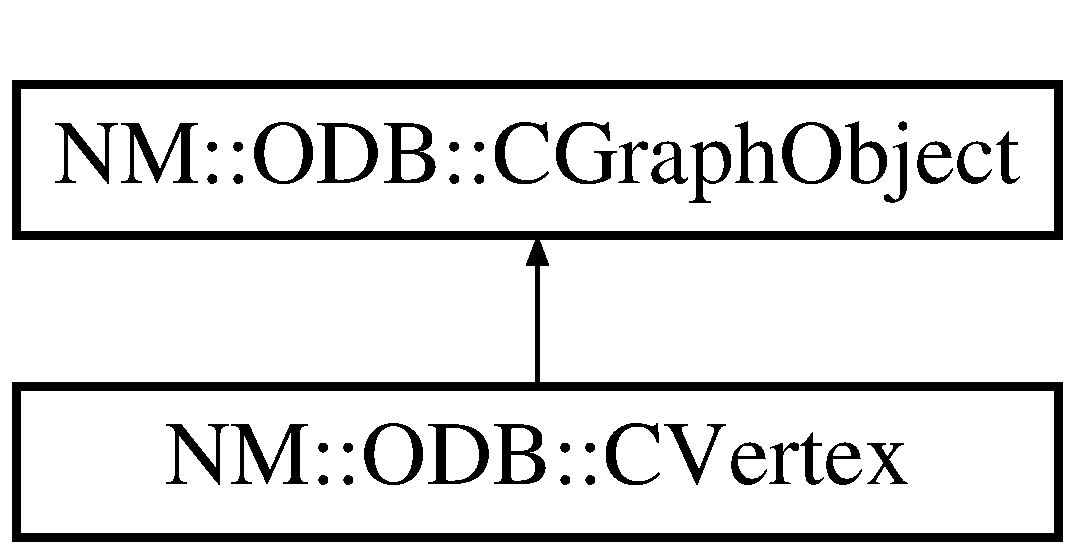
\includegraphics[height=2.000000cm]{class_n_m_1_1_o_d_b_1_1_c_vertex}
\end{center}
\end{figure}
\subsection*{Public Member Functions}
\begin{DoxyCompactItemize}
\item 
\hyperlink{class_n_m_1_1_o_d_b_1_1_c_vertex_a5e8a4fe9fda6040c0c0f28daf05bb03b}{C\+Vertex} ()
\item 
\hyperlink{class_n_m_1_1_o_d_b_1_1_c_vertex_a8e26e972a1324064e6706809ebf81377}{$\sim$\+C\+Vertex} ()
\item 
\hyperlink{class_n_m_1_1_o_d_b_1_1_c_vertex_aaa42a4697d7ad41b6f20f16a9fb96170}{C\+Vertex} (const \hyperlink{class_n_m_1_1_o_d_b_1_1_c_vertex}{C\+Vertex} \&o, const \hyperlink{namespace_n_m_1_1_o_d_b_a262b64fab56baaa96e18bac4ada88265}{O\+B\+J\+E\+C\+T\+U\+I\+D} New\+U\+I\+D)
\item 
\hyperlink{class_n_m_1_1_o_d_b_1_1_c_vertex}{C\+Vertex} $\ast$ \hyperlink{class_n_m_1_1_o_d_b_1_1_c_vertex_afe1a131c1b47dc9953e5d164a380af68}{clone} (size\+\_\+t new\+Object\+U\+I\+D) const 
\item 
bool \hyperlink{class_n_m_1_1_o_d_b_1_1_c_vertex_a5969c889748b2713e0b1742a136cdf05}{Point\+In\+Object} (int \&x, int \&y)
\end{DoxyCompactItemize}
\subsection*{Friends}
\begin{DoxyCompactItemize}
\item 
class \hyperlink{class_n_m_1_1_o_d_b_1_1_c_vertex_a1d86cbedc9bc2eb368c4ef78ee139e3d}{C\+Vertex\+Table}
\end{DoxyCompactItemize}
\subsection*{Additional Inherited Members}


\subsection{Detailed Description}
Class \hyperlink{class_n_m_1_1_o_d_b_1_1_c_vertex}{C\+Vertex} 

\subsection{Constructor \& Destructor Documentation}
\hypertarget{class_n_m_1_1_o_d_b_1_1_c_vertex_a5e8a4fe9fda6040c0c0f28daf05bb03b}{}\index{N\+M\+::\+O\+D\+B\+::\+C\+Vertex@{N\+M\+::\+O\+D\+B\+::\+C\+Vertex}!C\+Vertex@{C\+Vertex}}
\index{C\+Vertex@{C\+Vertex}!N\+M\+::\+O\+D\+B\+::\+C\+Vertex@{N\+M\+::\+O\+D\+B\+::\+C\+Vertex}}
\subsubsection[{C\+Vertex()}]{\setlength{\rightskip}{0pt plus 5cm}N\+M\+::\+O\+D\+B\+::\+C\+Vertex\+::\+C\+Vertex (
\begin{DoxyParamCaption}
{}
\end{DoxyParamCaption}
)\hspace{0.3cm}{\ttfamily [inline]}}\label{class_n_m_1_1_o_d_b_1_1_c_vertex_a5e8a4fe9fda6040c0c0f28daf05bb03b}
\hypertarget{class_n_m_1_1_o_d_b_1_1_c_vertex_a8e26e972a1324064e6706809ebf81377}{}\index{N\+M\+::\+O\+D\+B\+::\+C\+Vertex@{N\+M\+::\+O\+D\+B\+::\+C\+Vertex}!````~C\+Vertex@{$\sim$\+C\+Vertex}}
\index{````~C\+Vertex@{$\sim$\+C\+Vertex}!N\+M\+::\+O\+D\+B\+::\+C\+Vertex@{N\+M\+::\+O\+D\+B\+::\+C\+Vertex}}
\subsubsection[{$\sim$\+C\+Vertex()}]{\setlength{\rightskip}{0pt plus 5cm}N\+M\+::\+O\+D\+B\+::\+C\+Vertex\+::$\sim$\+C\+Vertex (
\begin{DoxyParamCaption}
{}
\end{DoxyParamCaption}
)\hspace{0.3cm}{\ttfamily [inline]}}\label{class_n_m_1_1_o_d_b_1_1_c_vertex_a8e26e972a1324064e6706809ebf81377}
\hypertarget{class_n_m_1_1_o_d_b_1_1_c_vertex_aaa42a4697d7ad41b6f20f16a9fb96170}{}\index{N\+M\+::\+O\+D\+B\+::\+C\+Vertex@{N\+M\+::\+O\+D\+B\+::\+C\+Vertex}!C\+Vertex@{C\+Vertex}}
\index{C\+Vertex@{C\+Vertex}!N\+M\+::\+O\+D\+B\+::\+C\+Vertex@{N\+M\+::\+O\+D\+B\+::\+C\+Vertex}}
\subsubsection[{C\+Vertex(const C\+Vertex \&o, const O\+B\+J\+E\+C\+T\+U\+I\+D New\+U\+I\+D)}]{\setlength{\rightskip}{0pt plus 5cm}N\+M\+::\+O\+D\+B\+::\+C\+Vertex\+::\+C\+Vertex (
\begin{DoxyParamCaption}
\item[{const {\bf C\+Vertex} \&}]{o, }
\item[{const {\bf O\+B\+J\+E\+C\+T\+U\+I\+D}}]{New\+U\+I\+D}
\end{DoxyParamCaption}
)\hspace{0.3cm}{\ttfamily [inline]}}\label{class_n_m_1_1_o_d_b_1_1_c_vertex_aaa42a4697d7ad41b6f20f16a9fb96170}


\subsection{Member Function Documentation}
\hypertarget{class_n_m_1_1_o_d_b_1_1_c_vertex_afe1a131c1b47dc9953e5d164a380af68}{}\index{N\+M\+::\+O\+D\+B\+::\+C\+Vertex@{N\+M\+::\+O\+D\+B\+::\+C\+Vertex}!clone@{clone}}
\index{clone@{clone}!N\+M\+::\+O\+D\+B\+::\+C\+Vertex@{N\+M\+::\+O\+D\+B\+::\+C\+Vertex}}
\subsubsection[{clone(size\+\_\+t new\+Object\+U\+I\+D) const }]{\setlength{\rightskip}{0pt plus 5cm}{\bf C\+Vertex}$\ast$ N\+M\+::\+O\+D\+B\+::\+C\+Vertex\+::clone (
\begin{DoxyParamCaption}
\item[{size\+\_\+t}]{new\+Object\+U\+I\+D}
\end{DoxyParamCaption}
) const\hspace{0.3cm}{\ttfamily [inline]}, {\ttfamily [virtual]}}\label{class_n_m_1_1_o_d_b_1_1_c_vertex_afe1a131c1b47dc9953e5d164a380af68}


Implements \hyperlink{class_n_m_1_1_o_d_b_1_1_c_graph_object_aa0ca9ee294c6b42e39fb2c3a6598b506}{N\+M\+::\+O\+D\+B\+::\+C\+Graph\+Object}.

\hypertarget{class_n_m_1_1_o_d_b_1_1_c_vertex_a5969c889748b2713e0b1742a136cdf05}{}\index{N\+M\+::\+O\+D\+B\+::\+C\+Vertex@{N\+M\+::\+O\+D\+B\+::\+C\+Vertex}!Point\+In\+Object@{Point\+In\+Object}}
\index{Point\+In\+Object@{Point\+In\+Object}!N\+M\+::\+O\+D\+B\+::\+C\+Vertex@{N\+M\+::\+O\+D\+B\+::\+C\+Vertex}}
\subsubsection[{Point\+In\+Object(int \&x, int \&y)}]{\setlength{\rightskip}{0pt plus 5cm}bool N\+M\+::\+O\+D\+B\+::\+C\+Vertex\+::\+Point\+In\+Object (
\begin{DoxyParamCaption}
\item[{int \&}]{x, }
\item[{int \&}]{y}
\end{DoxyParamCaption}
)\hspace{0.3cm}{\ttfamily [virtual]}}\label{class_n_m_1_1_o_d_b_1_1_c_vertex_a5969c889748b2713e0b1742a136cdf05}


Reimplemented from \hyperlink{class_n_m_1_1_o_d_b_1_1_c_graph_object_a8069a2286005ece610484b60ee8c0fde}{N\+M\+::\+O\+D\+B\+::\+C\+Graph\+Object}.



\subsection{Friends And Related Function Documentation}
\hypertarget{class_n_m_1_1_o_d_b_1_1_c_vertex_a1d86cbedc9bc2eb368c4ef78ee139e3d}{}\index{N\+M\+::\+O\+D\+B\+::\+C\+Vertex@{N\+M\+::\+O\+D\+B\+::\+C\+Vertex}!C\+Vertex\+Table@{C\+Vertex\+Table}}
\index{C\+Vertex\+Table@{C\+Vertex\+Table}!N\+M\+::\+O\+D\+B\+::\+C\+Vertex@{N\+M\+::\+O\+D\+B\+::\+C\+Vertex}}
\subsubsection[{C\+Vertex\+Table}]{\setlength{\rightskip}{0pt plus 5cm}friend class {\bf C\+Vertex\+Table}\hspace{0.3cm}{\ttfamily [friend]}}\label{class_n_m_1_1_o_d_b_1_1_c_vertex_a1d86cbedc9bc2eb368c4ef78ee139e3d}


The documentation for this class was generated from the following files\+:\begin{DoxyCompactItemize}
\item 
C\+:/\+Users/\+Simon/\+Documents/\+Personal/\+Source Code/\+Projects/\+Network\+Modeller/\+Object\+Database/\+Data\+Objects/\hyperlink{_graph_objects_8h}{Graph\+Objects.\+h}\item 
C\+:/\+Users/\+Simon/\+Documents/\+Personal/\+Source Code/\+Projects/\+Network\+Modeller/\+Object\+Database/\+Data\+Objects/\hyperlink{_graph_objects_8cpp}{Graph\+Objects.\+cpp}\end{DoxyCompactItemize}

\hypertarget{class_n_m_1_1_o_d_b_1_1_c_vertex_table}{}\section{N\+M\+:\+:O\+D\+B\+:\+:C\+Vertex\+Table Class Reference}
\label{class_n_m_1_1_o_d_b_1_1_c_vertex_table}\index{N\+M\+::\+O\+D\+B\+::\+C\+Vertex\+Table@{N\+M\+::\+O\+D\+B\+::\+C\+Vertex\+Table}}


{\ttfamily \#include $<$Vertex\+Table.\+h$>$}

Inheritance diagram for N\+M\+:\+:O\+D\+B\+:\+:C\+Vertex\+Table\+:\begin{figure}[H]
\begin{center}
\leavevmode
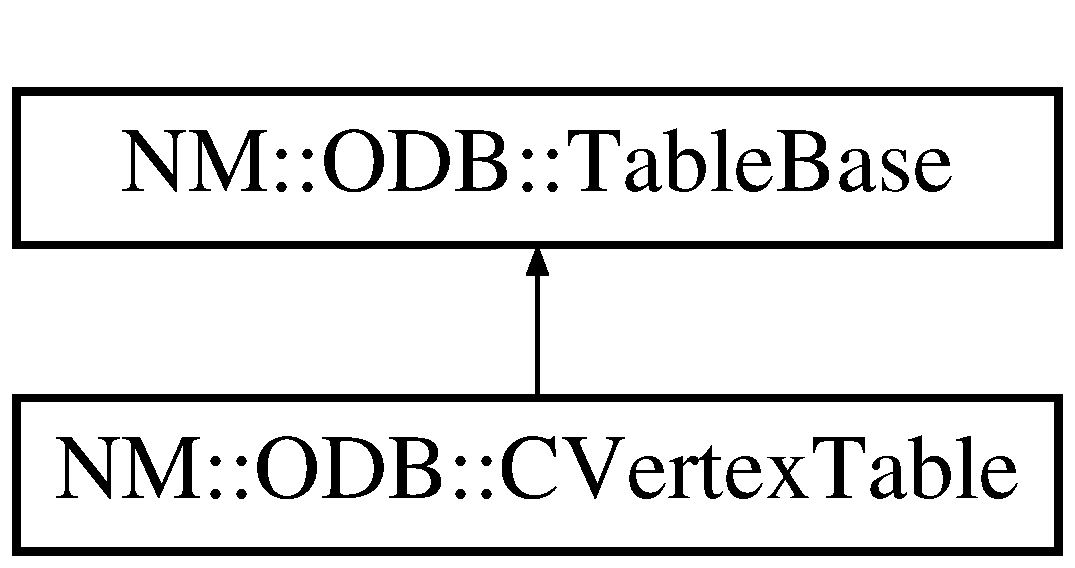
\includegraphics[height=2.000000cm]{class_n_m_1_1_o_d_b_1_1_c_vertex_table}
\end{center}
\end{figure}
\subsection*{Public Types}
\begin{DoxyCompactItemize}
\item 
typedef \+::std\+::vector$<$ \hyperlink{class_n_m_1_1_o_d_b_1_1_c_graph_object}{C\+Graph\+Object} $\ast$ $>$ \hyperlink{class_n_m_1_1_o_d_b_1_1_c_vertex_table_aad307ea0f7106397e4da74c082c3aaf7}{V\+E\+R\+T\+E\+X\+\_\+\+V\+E\+C\+T\+O\+R}
\end{DoxyCompactItemize}
\subsection*{Public Member Functions}
\begin{DoxyCompactItemize}
\item 
\hyperlink{class_n_m_1_1_o_d_b_1_1_c_vertex_table_a3862b9b2a29a5e43b7ef6dbee07e8836}{C\+Vertex\+Table} (\hyperlink{class_n_m_1_1_o_d_b_1_1_c_object_database}{C\+Object\+Database} $\ast$object\+Database, \hyperlink{class_n_m_1_1_o_d_b_1_1_c_graph_object_factory}{C\+Graph\+Object\+Factory} $\ast$object\+Factory)
\item 
\hyperlink{class_n_m_1_1_o_d_b_1_1_c_vertex_table_ae91221bed0ddbfe3bdb28d3526fa4b67}{$\sim$\+C\+Vertex\+Table} (void)
\item 
\hyperlink{namespace_n_m_1_1_o_d_b_a262b64fab56baaa96e18bac4ada88265}{O\+B\+J\+E\+C\+T\+U\+I\+D} \hyperlink{class_n_m_1_1_o_d_b_1_1_c_vertex_table_add5b10602223cd641b5dd503e86e0cbe}{Create\+Vertex} (\hyperlink{namespace_n_m_1_1_o_d_b_a74e0c94daaeea6f7e783c03a8c921022}{Vertex\+Type} vertex\+Type, \hyperlink{namespace_n_m_1_1_o_d_b_a8770283da9792324e1afe8104d40123b}{O\+B\+J\+E\+C\+T\+A\+T\+T\+R\+I\+B\+U\+T\+E\+S} $\ast$attribute\+Map I\+N, \hyperlink{class_n_m_1_1_o_d_b_1_1_c_graph_object}{C\+Graph\+Object} $\ast$$\ast$p\+Object O\+U\+T)
\item 
\hyperlink{namespace_n_m_1_1_o_d_b_a262b64fab56baaa96e18bac4ada88265}{O\+B\+J\+E\+C\+T\+U\+I\+D} \hyperlink{class_n_m_1_1_o_d_b_1_1_c_vertex_table_afb2bce5eba9132b17869930eac2b27df}{Copy\+Vertex} (\hyperlink{class_n_m_1_1_o_d_b_1_1_c_graph_object}{C\+Graph\+Object} $\ast$source\+Object I\+N, \hyperlink{namespace_n_m_1_1_o_d_b_a262b64fab56baaa96e18bac4ada88265}{O\+B\+J\+E\+C\+T\+U\+I\+D} dest\+Object\+U\+I\+D, \hyperlink{class_n_m_1_1_o_d_b_1_1_c_graph_object}{C\+Graph\+Object} $\ast$$\ast$p\+Object O\+U\+T)
\item 
bool \hyperlink{class_n_m_1_1_o_d_b_1_1_c_vertex_table_abe4bd94c203e37128e99c75afee8ea5c}{Destroy\+Vertex} (\hyperlink{class_n_m_1_1_o_d_b_1_1_c_graph_object}{C\+Graph\+Object} $\ast$p\+Object)
\item 
void \hyperlink{class_n_m_1_1_o_d_b_1_1_c_vertex_table_a86fcbaf8c65e5cb5d9963b5352120f7d}{Clear} ()
\item 
void \hyperlink{class_n_m_1_1_o_d_b_1_1_c_vertex_table_af00d1b7bfa9853437582121ab9b152a5}{Add\+Sibling} (\hyperlink{class_n_m_1_1_o_d_b_1_1_c_graph_object}{C\+Graph\+Object} $\ast$graph\+Object)
\item 
void \hyperlink{class_n_m_1_1_o_d_b_1_1_c_vertex_table_a1f133ede0be1de9c552d98820e06eed7}{Delete\+Sibling} (\hyperlink{class_n_m_1_1_o_d_b_1_1_c_graph_object}{C\+Graph\+Object} $\ast$graph\+Object)
\item 
\hyperlink{namespace_n_m_1_1_o_d_b_a262b64fab56baaa96e18bac4ada88265}{O\+B\+J\+E\+C\+T\+U\+I\+D} \hyperlink{class_n_m_1_1_o_d_b_1_1_c_vertex_table_a9dcc57ca073291f976037029ae2eb1b6}{Get\+Sibling} (\hyperlink{namespace_n_m_1_1_o_d_b_a74e0c94daaeea6f7e783c03a8c921022}{Vertex\+Type} v\+Type, \hyperlink{namespace_n_m_1_1_o_d_b_a1b474aa7e937112cda42381969dcb55e}{Sibling\+Position} position)
\item 
\hyperlink{class_n_m_1_1_o_d_b_1_1_c_vertex}{C\+Vertex} $\ast$ \hyperlink{class_n_m_1_1_o_d_b_1_1_c_vertex_table_ae3f7e93df587a2ad0241e06fb8641c9f}{Is\+In\+Vertex} (int x, int y)
\item 
bool \hyperlink{class_n_m_1_1_o_d_b_1_1_c_vertex_table_ad6c21c25a002804c3255771d15a513bf}{Set\+Value} (\hyperlink{class_n_m_1_1_o_d_b_1_1_c_graph_object}{C\+Graph\+Object} $\ast$, size\+\_\+t idx, \hyperlink{class_n_m_1_1_o_d_b_1_1_value}{Value} const \&v)
\item 
bool \hyperlink{class_n_m_1_1_o_d_b_1_1_c_vertex_table_a1433c9bce4a02925cf39e0d13ed4d19b}{Set\+Value} (\hyperlink{class_n_m_1_1_o_d_b_1_1_c_graph_object}{C\+Graph\+Object} $\ast$, const \+::std\+::wstring \&attrname, \hyperlink{class_n_m_1_1_o_d_b_1_1_value}{Value} const \&v)
\end{DoxyCompactItemize}
\subsection*{Public Attributes}
\begin{DoxyCompactItemize}
\item 
\hyperlink{class_n_m_1_1_o_d_b_1_1_c_vertex_table_aad307ea0f7106397e4da74c082c3aaf7}{V\+E\+R\+T\+E\+X\+\_\+\+V\+E\+C\+T\+O\+R} \hyperlink{class_n_m_1_1_o_d_b_1_1_c_vertex_table_af3e5fc03a2aa79bb8d4e2cac3f445a96}{verticies}
\end{DoxyCompactItemize}


\subsection{Member Typedef Documentation}
\hypertarget{class_n_m_1_1_o_d_b_1_1_c_vertex_table_aad307ea0f7106397e4da74c082c3aaf7}{}\index{N\+M\+::\+O\+D\+B\+::\+C\+Vertex\+Table@{N\+M\+::\+O\+D\+B\+::\+C\+Vertex\+Table}!V\+E\+R\+T\+E\+X\+\_\+\+V\+E\+C\+T\+O\+R@{V\+E\+R\+T\+E\+X\+\_\+\+V\+E\+C\+T\+O\+R}}
\index{V\+E\+R\+T\+E\+X\+\_\+\+V\+E\+C\+T\+O\+R@{V\+E\+R\+T\+E\+X\+\_\+\+V\+E\+C\+T\+O\+R}!N\+M\+::\+O\+D\+B\+::\+C\+Vertex\+Table@{N\+M\+::\+O\+D\+B\+::\+C\+Vertex\+Table}}
\subsubsection[{V\+E\+R\+T\+E\+X\+\_\+\+V\+E\+C\+T\+O\+R}]{\setlength{\rightskip}{0pt plus 5cm}typedef \+::std\+::vector$<${\bf C\+Graph\+Object}$\ast$$>$ {\bf N\+M\+::\+O\+D\+B\+::\+C\+Vertex\+Table\+::\+V\+E\+R\+T\+E\+X\+\_\+\+V\+E\+C\+T\+O\+R}}\label{class_n_m_1_1_o_d_b_1_1_c_vertex_table_aad307ea0f7106397e4da74c082c3aaf7}


\subsection{Constructor \& Destructor Documentation}
\hypertarget{class_n_m_1_1_o_d_b_1_1_c_vertex_table_a3862b9b2a29a5e43b7ef6dbee07e8836}{}\index{N\+M\+::\+O\+D\+B\+::\+C\+Vertex\+Table@{N\+M\+::\+O\+D\+B\+::\+C\+Vertex\+Table}!C\+Vertex\+Table@{C\+Vertex\+Table}}
\index{C\+Vertex\+Table@{C\+Vertex\+Table}!N\+M\+::\+O\+D\+B\+::\+C\+Vertex\+Table@{N\+M\+::\+O\+D\+B\+::\+C\+Vertex\+Table}}
\subsubsection[{C\+Vertex\+Table(\+C\+Object\+Database $\ast$object\+Database, C\+Graph\+Object\+Factory $\ast$object\+Factory)}]{\setlength{\rightskip}{0pt plus 5cm}N\+M\+::\+O\+D\+B\+::\+C\+Vertex\+Table\+::\+C\+Vertex\+Table (
\begin{DoxyParamCaption}
\item[{{\bf C\+Object\+Database} $\ast$}]{object\+Database, }
\item[{{\bf C\+Graph\+Object\+Factory} $\ast$}]{object\+Factory}
\end{DoxyParamCaption}
)\hspace{0.3cm}{\ttfamily [explicit]}}\label{class_n_m_1_1_o_d_b_1_1_c_vertex_table_a3862b9b2a29a5e43b7ef6dbee07e8836}
\hypertarget{class_n_m_1_1_o_d_b_1_1_c_vertex_table_ae91221bed0ddbfe3bdb28d3526fa4b67}{}\index{N\+M\+::\+O\+D\+B\+::\+C\+Vertex\+Table@{N\+M\+::\+O\+D\+B\+::\+C\+Vertex\+Table}!````~C\+Vertex\+Table@{$\sim$\+C\+Vertex\+Table}}
\index{````~C\+Vertex\+Table@{$\sim$\+C\+Vertex\+Table}!N\+M\+::\+O\+D\+B\+::\+C\+Vertex\+Table@{N\+M\+::\+O\+D\+B\+::\+C\+Vertex\+Table}}
\subsubsection[{$\sim$\+C\+Vertex\+Table(void)}]{\setlength{\rightskip}{0pt plus 5cm}N\+M\+::\+O\+D\+B\+::\+C\+Vertex\+Table\+::$\sim$\+C\+Vertex\+Table (
\begin{DoxyParamCaption}
\item[{void}]{}
\end{DoxyParamCaption}
)}\label{class_n_m_1_1_o_d_b_1_1_c_vertex_table_ae91221bed0ddbfe3bdb28d3526fa4b67}


\subsection{Member Function Documentation}
\hypertarget{class_n_m_1_1_o_d_b_1_1_c_vertex_table_af00d1b7bfa9853437582121ab9b152a5}{}\index{N\+M\+::\+O\+D\+B\+::\+C\+Vertex\+Table@{N\+M\+::\+O\+D\+B\+::\+C\+Vertex\+Table}!Add\+Sibling@{Add\+Sibling}}
\index{Add\+Sibling@{Add\+Sibling}!N\+M\+::\+O\+D\+B\+::\+C\+Vertex\+Table@{N\+M\+::\+O\+D\+B\+::\+C\+Vertex\+Table}}
\subsubsection[{Add\+Sibling(\+C\+Graph\+Object $\ast$graph\+Object)}]{\setlength{\rightskip}{0pt plus 5cm}void N\+M\+::\+O\+D\+B\+::\+C\+Vertex\+Table\+::\+Add\+Sibling (
\begin{DoxyParamCaption}
\item[{{\bf C\+Graph\+Object} $\ast$}]{graph\+Object}
\end{DoxyParamCaption}
)}\label{class_n_m_1_1_o_d_b_1_1_c_vertex_table_af00d1b7bfa9853437582121ab9b152a5}
\hypertarget{class_n_m_1_1_o_d_b_1_1_c_vertex_table_a86fcbaf8c65e5cb5d9963b5352120f7d}{}\index{N\+M\+::\+O\+D\+B\+::\+C\+Vertex\+Table@{N\+M\+::\+O\+D\+B\+::\+C\+Vertex\+Table}!Clear@{Clear}}
\index{Clear@{Clear}!N\+M\+::\+O\+D\+B\+::\+C\+Vertex\+Table@{N\+M\+::\+O\+D\+B\+::\+C\+Vertex\+Table}}
\subsubsection[{Clear()}]{\setlength{\rightskip}{0pt plus 5cm}void N\+M\+::\+O\+D\+B\+::\+C\+Vertex\+Table\+::\+Clear (
\begin{DoxyParamCaption}
\item[{void}]{}
\end{DoxyParamCaption}
)}\label{class_n_m_1_1_o_d_b_1_1_c_vertex_table_a86fcbaf8c65e5cb5d9963b5352120f7d}
\hypertarget{class_n_m_1_1_o_d_b_1_1_c_vertex_table_afb2bce5eba9132b17869930eac2b27df}{}\index{N\+M\+::\+O\+D\+B\+::\+C\+Vertex\+Table@{N\+M\+::\+O\+D\+B\+::\+C\+Vertex\+Table}!Copy\+Vertex@{Copy\+Vertex}}
\index{Copy\+Vertex@{Copy\+Vertex}!N\+M\+::\+O\+D\+B\+::\+C\+Vertex\+Table@{N\+M\+::\+O\+D\+B\+::\+C\+Vertex\+Table}}
\subsubsection[{Copy\+Vertex(\+C\+Graph\+Object $\ast$source\+Object I\+N, O\+B\+J\+E\+C\+T\+U\+I\+D dest\+Object\+U\+I\+D, C\+Graph\+Object $\ast$$\ast$p\+Object O\+U\+T)}]{\setlength{\rightskip}{0pt plus 5cm}{\bf O\+B\+J\+E\+C\+T\+U\+I\+D} N\+M\+::\+O\+D\+B\+::\+C\+Vertex\+Table\+::\+Copy\+Vertex (
\begin{DoxyParamCaption}
\item[{{\bf C\+Graph\+Object} $\ast$source\+Object}]{I\+N, }
\item[{{\bf O\+B\+J\+E\+C\+T\+U\+I\+D}}]{dest\+Object\+U\+I\+D, }
\item[{{\bf C\+Graph\+Object} $\ast$$\ast$p\+Object}]{O\+U\+T}
\end{DoxyParamCaption}
)}\label{class_n_m_1_1_o_d_b_1_1_c_vertex_table_afb2bce5eba9132b17869930eac2b27df}
\hypertarget{class_n_m_1_1_o_d_b_1_1_c_vertex_table_add5b10602223cd641b5dd503e86e0cbe}{}\index{N\+M\+::\+O\+D\+B\+::\+C\+Vertex\+Table@{N\+M\+::\+O\+D\+B\+::\+C\+Vertex\+Table}!Create\+Vertex@{Create\+Vertex}}
\index{Create\+Vertex@{Create\+Vertex}!N\+M\+::\+O\+D\+B\+::\+C\+Vertex\+Table@{N\+M\+::\+O\+D\+B\+::\+C\+Vertex\+Table}}
\subsubsection[{Create\+Vertex(\+Vertex\+Type vertex\+Type, O\+B\+J\+E\+C\+T\+A\+T\+T\+R\+I\+B\+U\+T\+E\+S $\ast$attribute\+Map I\+N, C\+Graph\+Object $\ast$$\ast$p\+Object O\+U\+T)}]{\setlength{\rightskip}{0pt plus 5cm}{\bf O\+B\+J\+E\+C\+T\+U\+I\+D} N\+M\+::\+O\+D\+B\+::\+C\+Vertex\+Table\+::\+Create\+Vertex (
\begin{DoxyParamCaption}
\item[{{\bf Vertex\+Type}}]{vertex\+Type, }
\item[{{\bf O\+B\+J\+E\+C\+T\+A\+T\+T\+R\+I\+B\+U\+T\+E\+S} $\ast$attribute\+Map}]{I\+N, }
\item[{{\bf C\+Graph\+Object} $\ast$$\ast$p\+Object}]{O\+U\+T}
\end{DoxyParamCaption}
)}\label{class_n_m_1_1_o_d_b_1_1_c_vertex_table_add5b10602223cd641b5dd503e86e0cbe}
\hypertarget{class_n_m_1_1_o_d_b_1_1_c_vertex_table_a1f133ede0be1de9c552d98820e06eed7}{}\index{N\+M\+::\+O\+D\+B\+::\+C\+Vertex\+Table@{N\+M\+::\+O\+D\+B\+::\+C\+Vertex\+Table}!Delete\+Sibling@{Delete\+Sibling}}
\index{Delete\+Sibling@{Delete\+Sibling}!N\+M\+::\+O\+D\+B\+::\+C\+Vertex\+Table@{N\+M\+::\+O\+D\+B\+::\+C\+Vertex\+Table}}
\subsubsection[{Delete\+Sibling(\+C\+Graph\+Object $\ast$graph\+Object)}]{\setlength{\rightskip}{0pt plus 5cm}void N\+M\+::\+O\+D\+B\+::\+C\+Vertex\+Table\+::\+Delete\+Sibling (
\begin{DoxyParamCaption}
\item[{{\bf C\+Graph\+Object} $\ast$}]{graph\+Object}
\end{DoxyParamCaption}
)}\label{class_n_m_1_1_o_d_b_1_1_c_vertex_table_a1f133ede0be1de9c552d98820e06eed7}
\hypertarget{class_n_m_1_1_o_d_b_1_1_c_vertex_table_abe4bd94c203e37128e99c75afee8ea5c}{}\index{N\+M\+::\+O\+D\+B\+::\+C\+Vertex\+Table@{N\+M\+::\+O\+D\+B\+::\+C\+Vertex\+Table}!Destroy\+Vertex@{Destroy\+Vertex}}
\index{Destroy\+Vertex@{Destroy\+Vertex}!N\+M\+::\+O\+D\+B\+::\+C\+Vertex\+Table@{N\+M\+::\+O\+D\+B\+::\+C\+Vertex\+Table}}
\subsubsection[{Destroy\+Vertex(\+C\+Graph\+Object $\ast$p\+Object)}]{\setlength{\rightskip}{0pt plus 5cm}bool N\+M\+::\+O\+D\+B\+::\+C\+Vertex\+Table\+::\+Destroy\+Vertex (
\begin{DoxyParamCaption}
\item[{{\bf C\+Graph\+Object} $\ast$}]{p\+Object}
\end{DoxyParamCaption}
)}\label{class_n_m_1_1_o_d_b_1_1_c_vertex_table_abe4bd94c203e37128e99c75afee8ea5c}
\hypertarget{class_n_m_1_1_o_d_b_1_1_c_vertex_table_a9dcc57ca073291f976037029ae2eb1b6}{}\index{N\+M\+::\+O\+D\+B\+::\+C\+Vertex\+Table@{N\+M\+::\+O\+D\+B\+::\+C\+Vertex\+Table}!Get\+Sibling@{Get\+Sibling}}
\index{Get\+Sibling@{Get\+Sibling}!N\+M\+::\+O\+D\+B\+::\+C\+Vertex\+Table@{N\+M\+::\+O\+D\+B\+::\+C\+Vertex\+Table}}
\subsubsection[{Get\+Sibling(\+Vertex\+Type v\+Type, Sibling\+Position position)}]{\setlength{\rightskip}{0pt plus 5cm}{\bf O\+B\+J\+E\+C\+T\+U\+I\+D} N\+M\+::\+O\+D\+B\+::\+C\+Vertex\+Table\+::\+Get\+Sibling (
\begin{DoxyParamCaption}
\item[{{\bf Vertex\+Type}}]{v\+Type, }
\item[{{\bf Sibling\+Position}}]{position}
\end{DoxyParamCaption}
)}\label{class_n_m_1_1_o_d_b_1_1_c_vertex_table_a9dcc57ca073291f976037029ae2eb1b6}
\hypertarget{class_n_m_1_1_o_d_b_1_1_c_vertex_table_ae3f7e93df587a2ad0241e06fb8641c9f}{}\index{N\+M\+::\+O\+D\+B\+::\+C\+Vertex\+Table@{N\+M\+::\+O\+D\+B\+::\+C\+Vertex\+Table}!Is\+In\+Vertex@{Is\+In\+Vertex}}
\index{Is\+In\+Vertex@{Is\+In\+Vertex}!N\+M\+::\+O\+D\+B\+::\+C\+Vertex\+Table@{N\+M\+::\+O\+D\+B\+::\+C\+Vertex\+Table}}
\subsubsection[{Is\+In\+Vertex(int x, int y)}]{\setlength{\rightskip}{0pt plus 5cm}{\bf C\+Vertex} $\ast$ N\+M\+::\+O\+D\+B\+::\+C\+Vertex\+Table\+::\+Is\+In\+Vertex (
\begin{DoxyParamCaption}
\item[{int}]{x, }
\item[{int}]{y}
\end{DoxyParamCaption}
)}\label{class_n_m_1_1_o_d_b_1_1_c_vertex_table_ae3f7e93df587a2ad0241e06fb8641c9f}
Is\+In\+Vertex -\/ needs to be moved outside of Vertex\+Table (Vertex\+Table) so its not having to access Object\+Database -\/ should be autonomous \hypertarget{class_n_m_1_1_o_d_b_1_1_c_vertex_table_ad6c21c25a002804c3255771d15a513bf}{}\index{N\+M\+::\+O\+D\+B\+::\+C\+Vertex\+Table@{N\+M\+::\+O\+D\+B\+::\+C\+Vertex\+Table}!Set\+Value@{Set\+Value}}
\index{Set\+Value@{Set\+Value}!N\+M\+::\+O\+D\+B\+::\+C\+Vertex\+Table@{N\+M\+::\+O\+D\+B\+::\+C\+Vertex\+Table}}
\subsubsection[{Set\+Value(\+C\+Graph\+Object $\ast$, size\+\_\+t idx, Value const \&v)}]{\setlength{\rightskip}{0pt plus 5cm}bool N\+M\+::\+O\+D\+B\+::\+C\+Vertex\+Table\+::\+Set\+Value (
\begin{DoxyParamCaption}
\item[{{\bf C\+Graph\+Object} $\ast$}]{vertex, }
\item[{size\+\_\+t}]{idx, }
\item[{{\bf Value} const \&}]{v}
\end{DoxyParamCaption}
)\hspace{0.3cm}{\ttfamily [virtual]}}\label{class_n_m_1_1_o_d_b_1_1_c_vertex_table_ad6c21c25a002804c3255771d15a513bf}


Implements \hyperlink{class_n_m_1_1_o_d_b_1_1_table_base_afbc340c36e140f2a8184d2585cc3b5d5}{N\+M\+::\+O\+D\+B\+::\+Table\+Base}.

\hypertarget{class_n_m_1_1_o_d_b_1_1_c_vertex_table_a1433c9bce4a02925cf39e0d13ed4d19b}{}\index{N\+M\+::\+O\+D\+B\+::\+C\+Vertex\+Table@{N\+M\+::\+O\+D\+B\+::\+C\+Vertex\+Table}!Set\+Value@{Set\+Value}}
\index{Set\+Value@{Set\+Value}!N\+M\+::\+O\+D\+B\+::\+C\+Vertex\+Table@{N\+M\+::\+O\+D\+B\+::\+C\+Vertex\+Table}}
\subsubsection[{Set\+Value(\+C\+Graph\+Object $\ast$, const \+::std\+::wstring \&attrname, Value const \&v)}]{\setlength{\rightskip}{0pt plus 5cm}bool N\+M\+::\+O\+D\+B\+::\+C\+Vertex\+Table\+::\+Set\+Value (
\begin{DoxyParamCaption}
\item[{{\bf C\+Graph\+Object} $\ast$}]{vertex, }
\item[{const \+::std\+::wstring \&}]{attrname, }
\item[{{\bf Value} const \&}]{v}
\end{DoxyParamCaption}
)\hspace{0.3cm}{\ttfamily [virtual]}}\label{class_n_m_1_1_o_d_b_1_1_c_vertex_table_a1433c9bce4a02925cf39e0d13ed4d19b}


Implements \hyperlink{class_n_m_1_1_o_d_b_1_1_table_base_a3e55bfe64ccdf81e6a96941b3f9a5fb4}{N\+M\+::\+O\+D\+B\+::\+Table\+Base}.



\subsection{Member Data Documentation}
\hypertarget{class_n_m_1_1_o_d_b_1_1_c_vertex_table_af3e5fc03a2aa79bb8d4e2cac3f445a96}{}\index{N\+M\+::\+O\+D\+B\+::\+C\+Vertex\+Table@{N\+M\+::\+O\+D\+B\+::\+C\+Vertex\+Table}!verticies@{verticies}}
\index{verticies@{verticies}!N\+M\+::\+O\+D\+B\+::\+C\+Vertex\+Table@{N\+M\+::\+O\+D\+B\+::\+C\+Vertex\+Table}}
\subsubsection[{verticies}]{\setlength{\rightskip}{0pt plus 5cm}{\bf V\+E\+R\+T\+E\+X\+\_\+\+V\+E\+C\+T\+O\+R} N\+M\+::\+O\+D\+B\+::\+C\+Vertex\+Table\+::verticies}\label{class_n_m_1_1_o_d_b_1_1_c_vertex_table_af3e5fc03a2aa79bb8d4e2cac3f445a96}


The documentation for this class was generated from the following files\+:\begin{DoxyCompactItemize}
\item 
C\+:/\+Users/\+Simon/\+Documents/\+Personal/\+Source Code/\+Projects/\+Network\+Modeller/\+Object\+Database/\+Tables/\hyperlink{_vertex_table_8h}{Vertex\+Table.\+h}\item 
C\+:/\+Users/\+Simon/\+Documents/\+Personal/\+Source Code/\+Projects/\+Network\+Modeller/\+Object\+Database/\+Tables/\hyperlink{_vertex_table_8cpp}{Vertex\+Table.\+cpp}\end{DoxyCompactItemize}

\hypertarget{class_n_m_1_1_o_d_b_1_1_database_notification_requests}{}\section{N\+M\+:\+:O\+D\+B\+:\+:Database\+Notification\+Requests Class Reference}
\label{class_n_m_1_1_o_d_b_1_1_database_notification_requests}\index{N\+M\+::\+O\+D\+B\+::\+Database\+Notification\+Requests@{N\+M\+::\+O\+D\+B\+::\+Database\+Notification\+Requests}}


{\ttfamily \#include $<$Database\+Notification\+Requests.\+h$>$}

\subsection*{Public Member Functions}
\begin{DoxyCompactItemize}
\item 
\hyperlink{class_n_m_1_1_o_d_b_1_1_database_notification_requests_aee52b22613d80f73e05e97635c8ad070}{$\sim$\+Database\+Notification\+Requests} (void)
\item 
void \hyperlink{class_n_m_1_1_o_d_b_1_1_database_notification_requests_aaec7b60add9cf7f77c607e8a56d19413}{Add\+Notification\+Request} (\hyperlink{class_n_m_1_1_o_d_b_1_1_c_database_observer}{C\+Database\+Observer} $\ast$p\+Observer, \hyperlink{namespace_n_m_1_1_o_d_b_ac9f60beb4a1c8a6240dd0c8baa281345}{Object\+Type},\+::std\+::vector$<$\+::std\+::wstring $>$ \&attribute\+\_\+list)
\item 
void \hyperlink{class_n_m_1_1_o_d_b_1_1_database_notification_requests_a25f0da2399287990dc4d597885d3c588}{Remove\+Notification\+Request} (\hyperlink{class_n_m_1_1_o_d_b_1_1_c_database_observer}{C\+Database\+Observer} $\ast$p\+Observer)
\item 
\+::std\+::set$<$ \hyperlink{class_n_m_1_1_o_d_b_1_1_c_database_observer}{C\+Database\+Observer} $\ast$ $>$ \hyperlink{class_n_m_1_1_o_d_b_1_1_database_notification_requests_aec57a4b7e864bbf9ed0a29402a55d10c}{Get\+Attribute\+Notification\+List} (\hyperlink{namespace_n_m_1_1_o_d_b_ac9f60beb4a1c8a6240dd0c8baa281345}{Object\+Type} object\+\_\+type,\+::std\+::wstring \&attribute)
\item 
bool \hyperlink{class_n_m_1_1_o_d_b_1_1_database_notification_requests_a9d5caa1bb9d4c07af7e1bb1d8be6d86f}{Is\+Object\+Attribute\+Update\+Registered} (\hyperlink{namespace_n_m_1_1_o_d_b_ac9f60beb4a1c8a6240dd0c8baa281345}{Object\+Type} object\+\_\+type,\+::std\+::wstring \&attribute)
\begin{DoxyCompactList}\small\item\em Boolean function to state if Object\+Type/\+Attribute combination is registered, not sure if we need this? \end{DoxyCompactList}\end{DoxyCompactItemize}
\subsection*{Static Public Member Functions}
\begin{DoxyCompactItemize}
\item 
static \hyperlink{class_n_m_1_1_o_d_b_1_1_database_notification_requests}{Database\+Notification\+Requests} $\ast$ \hyperlink{class_n_m_1_1_o_d_b_1_1_database_notification_requests_a5e9870a9abb510e510715dbcf3cb1fd9}{get\+Instance} ()
\end{DoxyCompactItemize}


\subsection{Constructor \& Destructor Documentation}
\hypertarget{class_n_m_1_1_o_d_b_1_1_database_notification_requests_aee52b22613d80f73e05e97635c8ad070}{}\index{N\+M\+::\+O\+D\+B\+::\+Database\+Notification\+Requests@{N\+M\+::\+O\+D\+B\+::\+Database\+Notification\+Requests}!````~Database\+Notification\+Requests@{$\sim$\+Database\+Notification\+Requests}}
\index{````~Database\+Notification\+Requests@{$\sim$\+Database\+Notification\+Requests}!N\+M\+::\+O\+D\+B\+::\+Database\+Notification\+Requests@{N\+M\+::\+O\+D\+B\+::\+Database\+Notification\+Requests}}
\subsubsection[{$\sim$\+Database\+Notification\+Requests(void)}]{\setlength{\rightskip}{0pt plus 5cm}N\+M\+::\+O\+D\+B\+::\+Database\+Notification\+Requests\+::$\sim$\+Database\+Notification\+Requests (
\begin{DoxyParamCaption}
\item[{void}]{}
\end{DoxyParamCaption}
)}\label{class_n_m_1_1_o_d_b_1_1_database_notification_requests_aee52b22613d80f73e05e97635c8ad070}


\subsection{Member Function Documentation}
\hypertarget{class_n_m_1_1_o_d_b_1_1_database_notification_requests_aaec7b60add9cf7f77c607e8a56d19413}{}\index{N\+M\+::\+O\+D\+B\+::\+Database\+Notification\+Requests@{N\+M\+::\+O\+D\+B\+::\+Database\+Notification\+Requests}!Add\+Notification\+Request@{Add\+Notification\+Request}}
\index{Add\+Notification\+Request@{Add\+Notification\+Request}!N\+M\+::\+O\+D\+B\+::\+Database\+Notification\+Requests@{N\+M\+::\+O\+D\+B\+::\+Database\+Notification\+Requests}}
\subsubsection[{Add\+Notification\+Request(\+C\+Database\+Observer $\ast$p\+Observer, Object\+Type,\+::std\+::vector$<$\+::std\+::wstring $>$ \&attribute\+\_\+list)}]{\setlength{\rightskip}{0pt plus 5cm}void N\+M\+::\+O\+D\+B\+::\+Database\+Notification\+Requests\+::\+Add\+Notification\+Request (
\begin{DoxyParamCaption}
\item[{{\bf C\+Database\+Observer} $\ast$}]{p\+Observer, }
\item[{{\bf Object\+Type}}]{object\+\_\+type, }
\item[{\+::std\+::vector$<$\+::std\+::wstring $>$ \&}]{attribute\+\_\+list}
\end{DoxyParamCaption}
)}\label{class_n_m_1_1_o_d_b_1_1_database_notification_requests_aaec7b60add9cf7f77c607e8a56d19413}
\hypertarget{class_n_m_1_1_o_d_b_1_1_database_notification_requests_aec57a4b7e864bbf9ed0a29402a55d10c}{}\index{N\+M\+::\+O\+D\+B\+::\+Database\+Notification\+Requests@{N\+M\+::\+O\+D\+B\+::\+Database\+Notification\+Requests}!Get\+Attribute\+Notification\+List@{Get\+Attribute\+Notification\+List}}
\index{Get\+Attribute\+Notification\+List@{Get\+Attribute\+Notification\+List}!N\+M\+::\+O\+D\+B\+::\+Database\+Notification\+Requests@{N\+M\+::\+O\+D\+B\+::\+Database\+Notification\+Requests}}
\subsubsection[{Get\+Attribute\+Notification\+List(\+Object\+Type object\+\_\+type,\+::std\+::wstring \&attribute)}]{\setlength{\rightskip}{0pt plus 5cm}std\+::set$<$ {\bf C\+Database\+Observer} $\ast$ $>$ N\+M\+::\+O\+D\+B\+::\+Database\+Notification\+Requests\+::\+Get\+Attribute\+Notification\+List (
\begin{DoxyParamCaption}
\item[{{\bf Object\+Type}}]{object\+\_\+type, }
\item[{\+::std\+::wstring \&}]{attribute}
\end{DoxyParamCaption}
)}\label{class_n_m_1_1_o_d_b_1_1_database_notification_requests_aec57a4b7e864bbf9ed0a29402a55d10c}
\hypertarget{class_n_m_1_1_o_d_b_1_1_database_notification_requests_a5e9870a9abb510e510715dbcf3cb1fd9}{}\index{N\+M\+::\+O\+D\+B\+::\+Database\+Notification\+Requests@{N\+M\+::\+O\+D\+B\+::\+Database\+Notification\+Requests}!get\+Instance@{get\+Instance}}
\index{get\+Instance@{get\+Instance}!N\+M\+::\+O\+D\+B\+::\+Database\+Notification\+Requests@{N\+M\+::\+O\+D\+B\+::\+Database\+Notification\+Requests}}
\subsubsection[{get\+Instance()}]{\setlength{\rightskip}{0pt plus 5cm}{\bf Database\+Notification\+Requests} $\ast$ N\+M\+::\+O\+D\+B\+::\+Database\+Notification\+Requests\+::get\+Instance (
\begin{DoxyParamCaption}
{}
\end{DoxyParamCaption}
)\hspace{0.3cm}{\ttfamily [static]}}\label{class_n_m_1_1_o_d_b_1_1_database_notification_requests_a5e9870a9abb510e510715dbcf3cb1fd9}
\hypertarget{class_n_m_1_1_o_d_b_1_1_database_notification_requests_a9d5caa1bb9d4c07af7e1bb1d8be6d86f}{}\index{N\+M\+::\+O\+D\+B\+::\+Database\+Notification\+Requests@{N\+M\+::\+O\+D\+B\+::\+Database\+Notification\+Requests}!Is\+Object\+Attribute\+Update\+Registered@{Is\+Object\+Attribute\+Update\+Registered}}
\index{Is\+Object\+Attribute\+Update\+Registered@{Is\+Object\+Attribute\+Update\+Registered}!N\+M\+::\+O\+D\+B\+::\+Database\+Notification\+Requests@{N\+M\+::\+O\+D\+B\+::\+Database\+Notification\+Requests}}
\subsubsection[{Is\+Object\+Attribute\+Update\+Registered(\+Object\+Type object\+\_\+type,\+::std\+::wstring \&attribute)}]{\setlength{\rightskip}{0pt plus 5cm}bool N\+M\+::\+O\+D\+B\+::\+Database\+Notification\+Requests\+::\+Is\+Object\+Attribute\+Update\+Registered (
\begin{DoxyParamCaption}
\item[{{\bf Object\+Type}}]{object\+\_\+type, }
\item[{\+::std\+::wstring \&}]{attribute}
\end{DoxyParamCaption}
)}\label{class_n_m_1_1_o_d_b_1_1_database_notification_requests_a9d5caa1bb9d4c07af7e1bb1d8be6d86f}


Boolean function to state if Object\+Type/\+Attribute combination is registered, not sure if we need this? 

\hypertarget{class_n_m_1_1_o_d_b_1_1_database_notification_requests_a25f0da2399287990dc4d597885d3c588}{}\index{N\+M\+::\+O\+D\+B\+::\+Database\+Notification\+Requests@{N\+M\+::\+O\+D\+B\+::\+Database\+Notification\+Requests}!Remove\+Notification\+Request@{Remove\+Notification\+Request}}
\index{Remove\+Notification\+Request@{Remove\+Notification\+Request}!N\+M\+::\+O\+D\+B\+::\+Database\+Notification\+Requests@{N\+M\+::\+O\+D\+B\+::\+Database\+Notification\+Requests}}
\subsubsection[{Remove\+Notification\+Request(\+C\+Database\+Observer $\ast$p\+Observer)}]{\setlength{\rightskip}{0pt plus 5cm}void N\+M\+::\+O\+D\+B\+::\+Database\+Notification\+Requests\+::\+Remove\+Notification\+Request (
\begin{DoxyParamCaption}
\item[{{\bf C\+Database\+Observer} $\ast$}]{p\+Observer}
\end{DoxyParamCaption}
)}\label{class_n_m_1_1_o_d_b_1_1_database_notification_requests_a25f0da2399287990dc4d597885d3c588}


The documentation for this class was generated from the following files\+:\begin{DoxyCompactItemize}
\item 
C\+:/\+Users/\+Simon/\+Documents/\+Personal/\+Source Code/\+Projects/\+Network\+Modeller/\+Object\+Database/\+Database\+Update\+Elements/\hyperlink{_database_notification_requests_8h}{Database\+Notification\+Requests.\+h}\item 
C\+:/\+Users/\+Simon/\+Documents/\+Personal/\+Source Code/\+Projects/\+Network\+Modeller/\+Object\+Database/\+Database\+Update\+Elements/\hyperlink{_database_notification_requests_8cpp}{Database\+Notification\+Requests.\+cpp}\end{DoxyCompactItemize}

\hypertarget{class_n_m_1_1_o_d_b_1_1_database_update_cache}{}\section{N\+M\+:\+:O\+D\+B\+:\+:Database\+Update\+Cache Class Reference}
\label{class_n_m_1_1_o_d_b_1_1_database_update_cache}\index{N\+M\+::\+O\+D\+B\+::\+Database\+Update\+Cache@{N\+M\+::\+O\+D\+B\+::\+Database\+Update\+Cache}}


{\ttfamily \#include $<$Database\+Update\+Cache.\+h$>$}

\subsection*{Public Types}
\begin{DoxyCompactItemize}
\item 
typedef \hyperlink{class_n_m_1_1_o_d_b_1_1_database_update_queue}{Database\+Update\+Queue} \hyperlink{class_n_m_1_1_o_d_b_1_1_database_update_cache_a3276437d24ef54dd3d31e2c27f34e84a}{queue}
\item 
typedef \hyperlink{class_n_m_1_1_o_d_b_1_1_database_update_cache_a3276437d24ef54dd3d31e2c27f34e84a}{queue} $\ast$ \hyperlink{class_n_m_1_1_o_d_b_1_1_database_update_cache_ae031bccefd897ef3c1d44a4e6c7ca99c}{queue\+\_\+ptr}
\end{DoxyCompactItemize}
\subsection*{Public Member Functions}
\begin{DoxyCompactItemize}
\item 
\hyperlink{class_n_m_1_1_o_d_b_1_1_database_update_cache_af064cf7160af5df46ebdd80d3df71434}{$\sim$\+Database\+Update\+Cache} (void)
\item 
void \hyperlink{class_n_m_1_1_o_d_b_1_1_database_update_cache_a2e906ecc8b45275c3f810afe40657a0f}{Insert\+Update} (\+::std\+::set$<$ \hyperlink{class_n_m_1_1_o_d_b_1_1_c_database_observer}{C\+Database\+Observer} $\ast$ $>$ \&, \hyperlink{class_n_m_1_1_o_d_b_1_1_database_update_record}{Database\+Update\+Record} \&)
\item 
void \hyperlink{class_n_m_1_1_o_d_b_1_1_database_update_cache_a69668e83a0c3ca8e6b9cdf9cc2e20a83}{Get\+Observer\+Queue} (I\+N \hyperlink{class_n_m_1_1_o_d_b_1_1_c_database_observer}{C\+Database\+Observer} $\ast$obs, I\+N O\+U\+T \hyperlink{class_n_m_1_1_o_d_b_1_1_database_update_queue}{Database\+Update\+Queue} $\ast$$\ast$pp\+Queue)
\item 
int \hyperlink{class_n_m_1_1_o_d_b_1_1_database_update_cache_af316bb9d19bcec424929e70f79ac81f1}{Get\+Observer\+Queue\+Size} (\hyperlink{class_n_m_1_1_o_d_b_1_1_c_database_observer}{C\+Database\+Observer} $\ast$)
\end{DoxyCompactItemize}
\subsection*{Static Public Member Functions}
\begin{DoxyCompactItemize}
\item 
static \hyperlink{class_n_m_1_1_o_d_b_1_1_database_update_cache}{Database\+Update\+Cache} $\ast$ \hyperlink{class_n_m_1_1_o_d_b_1_1_database_update_cache_a5fa9e7ca0980ec0a8f3a275a45d6c32d}{get\+Instance} ()
\end{DoxyCompactItemize}


\subsection{Member Typedef Documentation}
\hypertarget{class_n_m_1_1_o_d_b_1_1_database_update_cache_a3276437d24ef54dd3d31e2c27f34e84a}{}\index{N\+M\+::\+O\+D\+B\+::\+Database\+Update\+Cache@{N\+M\+::\+O\+D\+B\+::\+Database\+Update\+Cache}!queue@{queue}}
\index{queue@{queue}!N\+M\+::\+O\+D\+B\+::\+Database\+Update\+Cache@{N\+M\+::\+O\+D\+B\+::\+Database\+Update\+Cache}}
\subsubsection[{queue}]{\setlength{\rightskip}{0pt plus 5cm}typedef {\bf Database\+Update\+Queue} {\bf N\+M\+::\+O\+D\+B\+::\+Database\+Update\+Cache\+::queue}}\label{class_n_m_1_1_o_d_b_1_1_database_update_cache_a3276437d24ef54dd3d31e2c27f34e84a}
\hypertarget{class_n_m_1_1_o_d_b_1_1_database_update_cache_ae031bccefd897ef3c1d44a4e6c7ca99c}{}\index{N\+M\+::\+O\+D\+B\+::\+Database\+Update\+Cache@{N\+M\+::\+O\+D\+B\+::\+Database\+Update\+Cache}!queue\+\_\+ptr@{queue\+\_\+ptr}}
\index{queue\+\_\+ptr@{queue\+\_\+ptr}!N\+M\+::\+O\+D\+B\+::\+Database\+Update\+Cache@{N\+M\+::\+O\+D\+B\+::\+Database\+Update\+Cache}}
\subsubsection[{queue\+\_\+ptr}]{\setlength{\rightskip}{0pt plus 5cm}typedef {\bf queue}$\ast$ {\bf N\+M\+::\+O\+D\+B\+::\+Database\+Update\+Cache\+::queue\+\_\+ptr}}\label{class_n_m_1_1_o_d_b_1_1_database_update_cache_ae031bccefd897ef3c1d44a4e6c7ca99c}


\subsection{Constructor \& Destructor Documentation}
\hypertarget{class_n_m_1_1_o_d_b_1_1_database_update_cache_af064cf7160af5df46ebdd80d3df71434}{}\index{N\+M\+::\+O\+D\+B\+::\+Database\+Update\+Cache@{N\+M\+::\+O\+D\+B\+::\+Database\+Update\+Cache}!````~Database\+Update\+Cache@{$\sim$\+Database\+Update\+Cache}}
\index{````~Database\+Update\+Cache@{$\sim$\+Database\+Update\+Cache}!N\+M\+::\+O\+D\+B\+::\+Database\+Update\+Cache@{N\+M\+::\+O\+D\+B\+::\+Database\+Update\+Cache}}
\subsubsection[{$\sim$\+Database\+Update\+Cache(void)}]{\setlength{\rightskip}{0pt plus 5cm}N\+M\+::\+O\+D\+B\+::\+Database\+Update\+Cache\+::$\sim$\+Database\+Update\+Cache (
\begin{DoxyParamCaption}
\item[{void}]{}
\end{DoxyParamCaption}
)}\label{class_n_m_1_1_o_d_b_1_1_database_update_cache_af064cf7160af5df46ebdd80d3df71434}


\subsection{Member Function Documentation}
\hypertarget{class_n_m_1_1_o_d_b_1_1_database_update_cache_a5fa9e7ca0980ec0a8f3a275a45d6c32d}{}\index{N\+M\+::\+O\+D\+B\+::\+Database\+Update\+Cache@{N\+M\+::\+O\+D\+B\+::\+Database\+Update\+Cache}!get\+Instance@{get\+Instance}}
\index{get\+Instance@{get\+Instance}!N\+M\+::\+O\+D\+B\+::\+Database\+Update\+Cache@{N\+M\+::\+O\+D\+B\+::\+Database\+Update\+Cache}}
\subsubsection[{get\+Instance()}]{\setlength{\rightskip}{0pt plus 5cm}{\bf Database\+Update\+Cache} $\ast$ N\+M\+::\+O\+D\+B\+::\+Database\+Update\+Cache\+::get\+Instance (
\begin{DoxyParamCaption}
{}
\end{DoxyParamCaption}
)\hspace{0.3cm}{\ttfamily [static]}}\label{class_n_m_1_1_o_d_b_1_1_database_update_cache_a5fa9e7ca0980ec0a8f3a275a45d6c32d}
\hypertarget{class_n_m_1_1_o_d_b_1_1_database_update_cache_a69668e83a0c3ca8e6b9cdf9cc2e20a83}{}\index{N\+M\+::\+O\+D\+B\+::\+Database\+Update\+Cache@{N\+M\+::\+O\+D\+B\+::\+Database\+Update\+Cache}!Get\+Observer\+Queue@{Get\+Observer\+Queue}}
\index{Get\+Observer\+Queue@{Get\+Observer\+Queue}!N\+M\+::\+O\+D\+B\+::\+Database\+Update\+Cache@{N\+M\+::\+O\+D\+B\+::\+Database\+Update\+Cache}}
\subsubsection[{Get\+Observer\+Queue(\+I\+N C\+Database\+Observer $\ast$obs, I\+N O\+U\+T Database\+Update\+Queue $\ast$$\ast$pp\+Queue)}]{\setlength{\rightskip}{0pt plus 5cm}void N\+M\+::\+O\+D\+B\+::\+Database\+Update\+Cache\+::\+Get\+Observer\+Queue (
\begin{DoxyParamCaption}
\item[{I\+N {\bf C\+Database\+Observer} $\ast$}]{obs, }
\item[{I\+N O\+U\+T {\bf Database\+Update\+Queue} $\ast$$\ast$}]{pp\+Queue}
\end{DoxyParamCaption}
)}\label{class_n_m_1_1_o_d_b_1_1_database_update_cache_a69668e83a0c3ca8e6b9cdf9cc2e20a83}
\hypertarget{class_n_m_1_1_o_d_b_1_1_database_update_cache_af316bb9d19bcec424929e70f79ac81f1}{}\index{N\+M\+::\+O\+D\+B\+::\+Database\+Update\+Cache@{N\+M\+::\+O\+D\+B\+::\+Database\+Update\+Cache}!Get\+Observer\+Queue\+Size@{Get\+Observer\+Queue\+Size}}
\index{Get\+Observer\+Queue\+Size@{Get\+Observer\+Queue\+Size}!N\+M\+::\+O\+D\+B\+::\+Database\+Update\+Cache@{N\+M\+::\+O\+D\+B\+::\+Database\+Update\+Cache}}
\subsubsection[{Get\+Observer\+Queue\+Size(\+C\+Database\+Observer $\ast$)}]{\setlength{\rightskip}{0pt plus 5cm}int N\+M\+::\+O\+D\+B\+::\+Database\+Update\+Cache\+::\+Get\+Observer\+Queue\+Size (
\begin{DoxyParamCaption}
\item[{{\bf C\+Database\+Observer} $\ast$}]{obs}
\end{DoxyParamCaption}
)}\label{class_n_m_1_1_o_d_b_1_1_database_update_cache_af316bb9d19bcec424929e70f79ac81f1}
\hypertarget{class_n_m_1_1_o_d_b_1_1_database_update_cache_a2e906ecc8b45275c3f810afe40657a0f}{}\index{N\+M\+::\+O\+D\+B\+::\+Database\+Update\+Cache@{N\+M\+::\+O\+D\+B\+::\+Database\+Update\+Cache}!Insert\+Update@{Insert\+Update}}
\index{Insert\+Update@{Insert\+Update}!N\+M\+::\+O\+D\+B\+::\+Database\+Update\+Cache@{N\+M\+::\+O\+D\+B\+::\+Database\+Update\+Cache}}
\subsubsection[{Insert\+Update(\+::std\+::set$<$ C\+Database\+Observer $\ast$ $>$ \&, Database\+Update\+Record \&)}]{\setlength{\rightskip}{0pt plus 5cm}void N\+M\+::\+O\+D\+B\+::\+Database\+Update\+Cache\+::\+Insert\+Update (
\begin{DoxyParamCaption}
\item[{\+::std\+::set$<$ {\bf C\+Database\+Observer} $\ast$ $>$ \&}]{obs\+\_\+list, }
\item[{{\bf Database\+Update\+Record} \&}]{db\+\_\+update}
\end{DoxyParamCaption}
)}\label{class_n_m_1_1_o_d_b_1_1_database_update_cache_a2e906ecc8b45275c3f810afe40657a0f}


The documentation for this class was generated from the following files\+:\begin{DoxyCompactItemize}
\item 
C\+:/\+Users/\+Simon/\+Documents/\+Personal/\+Source Code/\+Projects/\+Network\+Modeller/\+Object\+Database/\+Database\+Update\+Elements/\hyperlink{_database_update_cache_8h}{Database\+Update\+Cache.\+h}\item 
C\+:/\+Users/\+Simon/\+Documents/\+Personal/\+Source Code/\+Projects/\+Network\+Modeller/\+Object\+Database/\+Database\+Update\+Elements/\hyperlink{_database_update_cache_8cpp}{Database\+Update\+Cache.\+cpp}\end{DoxyCompactItemize}

\hypertarget{class_n_m_1_1_o_d_b_1_1_database_update_queue}{}\section{N\+M\+:\+:O\+D\+B\+:\+:Database\+Update\+Queue Class Reference}
\label{class_n_m_1_1_o_d_b_1_1_database_update_queue}\index{N\+M\+::\+O\+D\+B\+::\+Database\+Update\+Queue@{N\+M\+::\+O\+D\+B\+::\+Database\+Update\+Queue}}


{\ttfamily \#include $<$Database\+Update\+Queue.\+h$>$}

\subsection*{Classes}
\begin{DoxyCompactItemize}
\item 
class \hyperlink{class_n_m_1_1_o_d_b_1_1_database_update_queue_1_1iterator}{iterator}
\end{DoxyCompactItemize}
\subsection*{Public Types}
\begin{DoxyCompactItemize}
\item 
typedef int \hyperlink{class_n_m_1_1_o_d_b_1_1_database_update_queue_a4a9f68d39b323a940c57db62b8f51506}{size\+\_\+type}
\end{DoxyCompactItemize}
\subsection*{Public Member Functions}
\begin{DoxyCompactItemize}
\item 
\hyperlink{class_n_m_1_1_o_d_b_1_1_database_update_queue_a53aee55e64568b652228f07a3328c0b4}{Database\+Update\+Queue} (void)
\item 
\hyperlink{class_n_m_1_1_o_d_b_1_1_database_update_queue_a6991cbfec3d4bd69e521d0aeac00256e}{Database\+Update\+Queue} (const \hyperlink{class_n_m_1_1_o_d_b_1_1_database_update_queue}{Database\+Update\+Queue} \&rhs)
\item 
\hyperlink{class_n_m_1_1_o_d_b_1_1_database_update_queue_a10c4fb2d1024ddb81ff46915f7204274}{$\sim$\+Database\+Update\+Queue} (void)
\item 
void \hyperlink{class_n_m_1_1_o_d_b_1_1_database_update_queue_ac45bbcc2e9fa0982b92dc1a07936c611}{Insert\+Update} (\hyperlink{class_n_m_1_1_o_d_b_1_1_database_update_record}{Database\+Update\+Record} \&update\+\_\+record)
\item 
void \hyperlink{class_n_m_1_1_o_d_b_1_1_database_update_queue_aa3eb3ca84792c938b6301b2d7e2ee6e9}{Lock} ()
\item 
bool \hyperlink{class_n_m_1_1_o_d_b_1_1_database_update_queue_a6a6c978a185e3b57abd5505518a44913}{Is\+Locked} ()
\item 
void \hyperlink{class_n_m_1_1_o_d_b_1_1_database_update_queue_a2665795812f2709d61f5a12ce813c063}{Clear} ()
\item 
int \hyperlink{class_n_m_1_1_o_d_b_1_1_database_update_queue_a40c3037ec070e8047091b7000e07cbe1}{Get\+Queue\+Size} ()
\item 
\hyperlink{class_n_m_1_1_o_d_b_1_1_database_update_queue_1_1iterator}{iterator} \hyperlink{class_n_m_1_1_o_d_b_1_1_database_update_queue_af199902f2ccc0435cb3ccd279964730a}{Begin} ()
\item 
\hyperlink{class_n_m_1_1_o_d_b_1_1_database_update_queue_1_1iterator}{iterator} \hyperlink{class_n_m_1_1_o_d_b_1_1_database_update_queue_a32679f2ab7a81338eb1852a15b844eca}{End} ()
\item 
\hyperlink{class_n_m_1_1_o_d_b_1_1_database_update_queue_a4a9f68d39b323a940c57db62b8f51506}{size\+\_\+type} \hyperlink{class_n_m_1_1_o_d_b_1_1_database_update_queue_ae40185ad2cae4e8a1def540e9957526d}{Size} ()
\end{DoxyCompactItemize}


\subsection{Member Typedef Documentation}
\hypertarget{class_n_m_1_1_o_d_b_1_1_database_update_queue_a4a9f68d39b323a940c57db62b8f51506}{}\index{N\+M\+::\+O\+D\+B\+::\+Database\+Update\+Queue@{N\+M\+::\+O\+D\+B\+::\+Database\+Update\+Queue}!size\+\_\+type@{size\+\_\+type}}
\index{size\+\_\+type@{size\+\_\+type}!N\+M\+::\+O\+D\+B\+::\+Database\+Update\+Queue@{N\+M\+::\+O\+D\+B\+::\+Database\+Update\+Queue}}
\subsubsection[{size\+\_\+type}]{\setlength{\rightskip}{0pt plus 5cm}typedef int {\bf N\+M\+::\+O\+D\+B\+::\+Database\+Update\+Queue\+::size\+\_\+type}}\label{class_n_m_1_1_o_d_b_1_1_database_update_queue_a4a9f68d39b323a940c57db62b8f51506}


\subsection{Constructor \& Destructor Documentation}
\hypertarget{class_n_m_1_1_o_d_b_1_1_database_update_queue_a53aee55e64568b652228f07a3328c0b4}{}\index{N\+M\+::\+O\+D\+B\+::\+Database\+Update\+Queue@{N\+M\+::\+O\+D\+B\+::\+Database\+Update\+Queue}!Database\+Update\+Queue@{Database\+Update\+Queue}}
\index{Database\+Update\+Queue@{Database\+Update\+Queue}!N\+M\+::\+O\+D\+B\+::\+Database\+Update\+Queue@{N\+M\+::\+O\+D\+B\+::\+Database\+Update\+Queue}}
\subsubsection[{Database\+Update\+Queue(void)}]{\setlength{\rightskip}{0pt plus 5cm}N\+M\+::\+O\+D\+B\+::\+Database\+Update\+Queue\+::\+Database\+Update\+Queue (
\begin{DoxyParamCaption}
\item[{void}]{}
\end{DoxyParamCaption}
)}\label{class_n_m_1_1_o_d_b_1_1_database_update_queue_a53aee55e64568b652228f07a3328c0b4}
\hypertarget{class_n_m_1_1_o_d_b_1_1_database_update_queue_a6991cbfec3d4bd69e521d0aeac00256e}{}\index{N\+M\+::\+O\+D\+B\+::\+Database\+Update\+Queue@{N\+M\+::\+O\+D\+B\+::\+Database\+Update\+Queue}!Database\+Update\+Queue@{Database\+Update\+Queue}}
\index{Database\+Update\+Queue@{Database\+Update\+Queue}!N\+M\+::\+O\+D\+B\+::\+Database\+Update\+Queue@{N\+M\+::\+O\+D\+B\+::\+Database\+Update\+Queue}}
\subsubsection[{Database\+Update\+Queue(const Database\+Update\+Queue \&rhs)}]{\setlength{\rightskip}{0pt plus 5cm}N\+M\+::\+O\+D\+B\+::\+Database\+Update\+Queue\+::\+Database\+Update\+Queue (
\begin{DoxyParamCaption}
\item[{const {\bf Database\+Update\+Queue} \&}]{rhs}
\end{DoxyParamCaption}
)}\label{class_n_m_1_1_o_d_b_1_1_database_update_queue_a6991cbfec3d4bd69e521d0aeac00256e}
\hypertarget{class_n_m_1_1_o_d_b_1_1_database_update_queue_a10c4fb2d1024ddb81ff46915f7204274}{}\index{N\+M\+::\+O\+D\+B\+::\+Database\+Update\+Queue@{N\+M\+::\+O\+D\+B\+::\+Database\+Update\+Queue}!````~Database\+Update\+Queue@{$\sim$\+Database\+Update\+Queue}}
\index{````~Database\+Update\+Queue@{$\sim$\+Database\+Update\+Queue}!N\+M\+::\+O\+D\+B\+::\+Database\+Update\+Queue@{N\+M\+::\+O\+D\+B\+::\+Database\+Update\+Queue}}
\subsubsection[{$\sim$\+Database\+Update\+Queue(void)}]{\setlength{\rightskip}{0pt plus 5cm}N\+M\+::\+O\+D\+B\+::\+Database\+Update\+Queue\+::$\sim$\+Database\+Update\+Queue (
\begin{DoxyParamCaption}
\item[{void}]{}
\end{DoxyParamCaption}
)}\label{class_n_m_1_1_o_d_b_1_1_database_update_queue_a10c4fb2d1024ddb81ff46915f7204274}


\subsection{Member Function Documentation}
\hypertarget{class_n_m_1_1_o_d_b_1_1_database_update_queue_af199902f2ccc0435cb3ccd279964730a}{}\index{N\+M\+::\+O\+D\+B\+::\+Database\+Update\+Queue@{N\+M\+::\+O\+D\+B\+::\+Database\+Update\+Queue}!Begin@{Begin}}
\index{Begin@{Begin}!N\+M\+::\+O\+D\+B\+::\+Database\+Update\+Queue@{N\+M\+::\+O\+D\+B\+::\+Database\+Update\+Queue}}
\subsubsection[{Begin()}]{\setlength{\rightskip}{0pt plus 5cm}{\bf iterator} N\+M\+::\+O\+D\+B\+::\+Database\+Update\+Queue\+::\+Begin (
\begin{DoxyParamCaption}
{}
\end{DoxyParamCaption}
)\hspace{0.3cm}{\ttfamily [inline]}}\label{class_n_m_1_1_o_d_b_1_1_database_update_queue_af199902f2ccc0435cb3ccd279964730a}
\hypertarget{class_n_m_1_1_o_d_b_1_1_database_update_queue_a2665795812f2709d61f5a12ce813c063}{}\index{N\+M\+::\+O\+D\+B\+::\+Database\+Update\+Queue@{N\+M\+::\+O\+D\+B\+::\+Database\+Update\+Queue}!Clear@{Clear}}
\index{Clear@{Clear}!N\+M\+::\+O\+D\+B\+::\+Database\+Update\+Queue@{N\+M\+::\+O\+D\+B\+::\+Database\+Update\+Queue}}
\subsubsection[{Clear()}]{\setlength{\rightskip}{0pt plus 5cm}void N\+M\+::\+O\+D\+B\+::\+Database\+Update\+Queue\+::\+Clear (
\begin{DoxyParamCaption}
{}
\end{DoxyParamCaption}
)}\label{class_n_m_1_1_o_d_b_1_1_database_update_queue_a2665795812f2709d61f5a12ce813c063}
\hypertarget{class_n_m_1_1_o_d_b_1_1_database_update_queue_a32679f2ab7a81338eb1852a15b844eca}{}\index{N\+M\+::\+O\+D\+B\+::\+Database\+Update\+Queue@{N\+M\+::\+O\+D\+B\+::\+Database\+Update\+Queue}!End@{End}}
\index{End@{End}!N\+M\+::\+O\+D\+B\+::\+Database\+Update\+Queue@{N\+M\+::\+O\+D\+B\+::\+Database\+Update\+Queue}}
\subsubsection[{End()}]{\setlength{\rightskip}{0pt plus 5cm}{\bf iterator} N\+M\+::\+O\+D\+B\+::\+Database\+Update\+Queue\+::\+End (
\begin{DoxyParamCaption}
{}
\end{DoxyParamCaption}
)}\label{class_n_m_1_1_o_d_b_1_1_database_update_queue_a32679f2ab7a81338eb1852a15b844eca}
\hypertarget{class_n_m_1_1_o_d_b_1_1_database_update_queue_a40c3037ec070e8047091b7000e07cbe1}{}\index{N\+M\+::\+O\+D\+B\+::\+Database\+Update\+Queue@{N\+M\+::\+O\+D\+B\+::\+Database\+Update\+Queue}!Get\+Queue\+Size@{Get\+Queue\+Size}}
\index{Get\+Queue\+Size@{Get\+Queue\+Size}!N\+M\+::\+O\+D\+B\+::\+Database\+Update\+Queue@{N\+M\+::\+O\+D\+B\+::\+Database\+Update\+Queue}}
\subsubsection[{Get\+Queue\+Size()}]{\setlength{\rightskip}{0pt plus 5cm}int N\+M\+::\+O\+D\+B\+::\+Database\+Update\+Queue\+::\+Get\+Queue\+Size (
\begin{DoxyParamCaption}
{}
\end{DoxyParamCaption}
)}\label{class_n_m_1_1_o_d_b_1_1_database_update_queue_a40c3037ec070e8047091b7000e07cbe1}
\hypertarget{class_n_m_1_1_o_d_b_1_1_database_update_queue_ac45bbcc2e9fa0982b92dc1a07936c611}{}\index{N\+M\+::\+O\+D\+B\+::\+Database\+Update\+Queue@{N\+M\+::\+O\+D\+B\+::\+Database\+Update\+Queue}!Insert\+Update@{Insert\+Update}}
\index{Insert\+Update@{Insert\+Update}!N\+M\+::\+O\+D\+B\+::\+Database\+Update\+Queue@{N\+M\+::\+O\+D\+B\+::\+Database\+Update\+Queue}}
\subsubsection[{Insert\+Update(\+Database\+Update\+Record \&update\+\_\+record)}]{\setlength{\rightskip}{0pt plus 5cm}void N\+M\+::\+O\+D\+B\+::\+Database\+Update\+Queue\+::\+Insert\+Update (
\begin{DoxyParamCaption}
\item[{{\bf Database\+Update\+Record} \&}]{update\+\_\+record}
\end{DoxyParamCaption}
)}\label{class_n_m_1_1_o_d_b_1_1_database_update_queue_ac45bbcc2e9fa0982b92dc1a07936c611}
\hypertarget{class_n_m_1_1_o_d_b_1_1_database_update_queue_a6a6c978a185e3b57abd5505518a44913}{}\index{N\+M\+::\+O\+D\+B\+::\+Database\+Update\+Queue@{N\+M\+::\+O\+D\+B\+::\+Database\+Update\+Queue}!Is\+Locked@{Is\+Locked}}
\index{Is\+Locked@{Is\+Locked}!N\+M\+::\+O\+D\+B\+::\+Database\+Update\+Queue@{N\+M\+::\+O\+D\+B\+::\+Database\+Update\+Queue}}
\subsubsection[{Is\+Locked()}]{\setlength{\rightskip}{0pt plus 5cm}bool N\+M\+::\+O\+D\+B\+::\+Database\+Update\+Queue\+::\+Is\+Locked (
\begin{DoxyParamCaption}
{}
\end{DoxyParamCaption}
)}\label{class_n_m_1_1_o_d_b_1_1_database_update_queue_a6a6c978a185e3b57abd5505518a44913}
\hypertarget{class_n_m_1_1_o_d_b_1_1_database_update_queue_aa3eb3ca84792c938b6301b2d7e2ee6e9}{}\index{N\+M\+::\+O\+D\+B\+::\+Database\+Update\+Queue@{N\+M\+::\+O\+D\+B\+::\+Database\+Update\+Queue}!Lock@{Lock}}
\index{Lock@{Lock}!N\+M\+::\+O\+D\+B\+::\+Database\+Update\+Queue@{N\+M\+::\+O\+D\+B\+::\+Database\+Update\+Queue}}
\subsubsection[{Lock()}]{\setlength{\rightskip}{0pt plus 5cm}void N\+M\+::\+O\+D\+B\+::\+Database\+Update\+Queue\+::\+Lock (
\begin{DoxyParamCaption}
{}
\end{DoxyParamCaption}
)}\label{class_n_m_1_1_o_d_b_1_1_database_update_queue_aa3eb3ca84792c938b6301b2d7e2ee6e9}
\hypertarget{class_n_m_1_1_o_d_b_1_1_database_update_queue_ae40185ad2cae4e8a1def540e9957526d}{}\index{N\+M\+::\+O\+D\+B\+::\+Database\+Update\+Queue@{N\+M\+::\+O\+D\+B\+::\+Database\+Update\+Queue}!Size@{Size}}
\index{Size@{Size}!N\+M\+::\+O\+D\+B\+::\+Database\+Update\+Queue@{N\+M\+::\+O\+D\+B\+::\+Database\+Update\+Queue}}
\subsubsection[{Size()}]{\setlength{\rightskip}{0pt plus 5cm}{\bf size\+\_\+type} N\+M\+::\+O\+D\+B\+::\+Database\+Update\+Queue\+::\+Size (
\begin{DoxyParamCaption}
{}
\end{DoxyParamCaption}
)}\label{class_n_m_1_1_o_d_b_1_1_database_update_queue_ae40185ad2cae4e8a1def540e9957526d}


The documentation for this class was generated from the following files\+:\begin{DoxyCompactItemize}
\item 
C\+:/\+Users/\+Simon/\+Documents/\+Personal/\+Source Code/\+Projects/\+Network\+Modeller/\+Object\+Database/\+Database\+Update\+Elements/\hyperlink{_database_update_queue_8h}{Database\+Update\+Queue.\+h}\item 
C\+:/\+Users/\+Simon/\+Documents/\+Personal/\+Source Code/\+Projects/\+Network\+Modeller/\+Object\+Database/\+Database\+Update\+Elements/\hyperlink{_database_update_queue_8cpp}{Database\+Update\+Queue.\+cpp}\end{DoxyCompactItemize}

\hypertarget{class_n_m_1_1_o_d_b_1_1_database_update_record}{}\section{N\+M\+:\+:O\+D\+B\+:\+:Database\+Update\+Record Class Reference}
\label{class_n_m_1_1_o_d_b_1_1_database_update_record}\index{N\+M\+::\+O\+D\+B\+::\+Database\+Update\+Record@{N\+M\+::\+O\+D\+B\+::\+Database\+Update\+Record}}


{\ttfamily \#include $<$Database\+Update\+Record.\+h$>$}

\subsection*{Public Member Functions}
\begin{DoxyCompactItemize}
\item 
\hyperlink{class_n_m_1_1_o_d_b_1_1_database_update_record_a55b1eac94cc7cadc239823269c714c84}{Database\+Update\+Record} (\hyperlink{namespace_n_m_1_1_o_d_b_a66aebefa38a81f7eeb64526035e77dfa}{Database\+Update\+Type} update\+\_\+type, int object\+\_\+id,\+::std\+::wstring \&object\+\_\+attribute\+\_\+name, \hyperlink{class_n_m_1_1_o_d_b_1_1_value}{Value} \&previous\+\_\+value, const \hyperlink{class_n_m_1_1_o_d_b_1_1_value}{Value} \&new\+\_\+value)
\item 
\hyperlink{class_n_m_1_1_o_d_b_1_1_database_update_record_a6ff2323d94a1a773d9bcc503a20385df}{Database\+Update\+Record} (const \hyperlink{class_n_m_1_1_o_d_b_1_1_database_update_record}{Database\+Update\+Record} \&rhs)
\item 
\hyperlink{class_n_m_1_1_o_d_b_1_1_database_update_record_a0d02938f5938d69efe62e30ad4d20a96}{$\sim$\+Database\+Update\+Record} (void)
\item 
\hyperlink{namespace_n_m_1_1_o_d_b_a66aebefa38a81f7eeb64526035e77dfa}{Database\+Update\+Type} \hyperlink{class_n_m_1_1_o_d_b_1_1_database_update_record_aa71854661082f55b4fc99a33d90153bd}{Get\+Update\+Type} () const 
\item 
int \hyperlink{class_n_m_1_1_o_d_b_1_1_database_update_record_a256ab628138040a2603109952c624b54}{Get\+Object\+Id} () const 
\item 
\+::std\+::wstring \hyperlink{class_n_m_1_1_o_d_b_1_1_database_update_record_ab9503ddc927d5eeea471a5fc64fafc1b}{Get\+Object\+Attribute\+Name} () const 
\item 
\hyperlink{class_n_m_1_1_o_d_b_1_1_value}{Value} \hyperlink{class_n_m_1_1_o_d_b_1_1_database_update_record_a980977f382c92c61ade77f4cc0d4e91e}{Get\+Previous\+Value} () const 
\item 
\hyperlink{class_n_m_1_1_o_d_b_1_1_value}{Value} \hyperlink{class_n_m_1_1_o_d_b_1_1_database_update_record_a8bf0b685f4075df49f58aaa01866cfec}{Get\+New\+Value} () const 
\end{DoxyCompactItemize}


\subsection{Constructor \& Destructor Documentation}
\hypertarget{class_n_m_1_1_o_d_b_1_1_database_update_record_a55b1eac94cc7cadc239823269c714c84}{}\index{N\+M\+::\+O\+D\+B\+::\+Database\+Update\+Record@{N\+M\+::\+O\+D\+B\+::\+Database\+Update\+Record}!Database\+Update\+Record@{Database\+Update\+Record}}
\index{Database\+Update\+Record@{Database\+Update\+Record}!N\+M\+::\+O\+D\+B\+::\+Database\+Update\+Record@{N\+M\+::\+O\+D\+B\+::\+Database\+Update\+Record}}
\subsubsection[{Database\+Update\+Record(\+Database\+Update\+Type update\+\_\+type, int object\+\_\+id,\+::std\+::wstring \&object\+\_\+attribute\+\_\+name, Value \&previous\+\_\+value, const Value \&new\+\_\+value)}]{\setlength{\rightskip}{0pt plus 5cm}N\+M\+::\+O\+D\+B\+::\+Database\+Update\+Record\+::\+Database\+Update\+Record (
\begin{DoxyParamCaption}
\item[{{\bf Database\+Update\+Type}}]{update\+\_\+type, }
\item[{int}]{object\+\_\+id, }
\item[{\+::std\+::wstring \&}]{object\+\_\+attribute\+\_\+name, }
\item[{{\bf Value} \&}]{previous\+\_\+value, }
\item[{const {\bf Value} \&}]{new\+\_\+value}
\end{DoxyParamCaption}
)}\label{class_n_m_1_1_o_d_b_1_1_database_update_record_a55b1eac94cc7cadc239823269c714c84}
\hypertarget{class_n_m_1_1_o_d_b_1_1_database_update_record_a6ff2323d94a1a773d9bcc503a20385df}{}\index{N\+M\+::\+O\+D\+B\+::\+Database\+Update\+Record@{N\+M\+::\+O\+D\+B\+::\+Database\+Update\+Record}!Database\+Update\+Record@{Database\+Update\+Record}}
\index{Database\+Update\+Record@{Database\+Update\+Record}!N\+M\+::\+O\+D\+B\+::\+Database\+Update\+Record@{N\+M\+::\+O\+D\+B\+::\+Database\+Update\+Record}}
\subsubsection[{Database\+Update\+Record(const Database\+Update\+Record \&rhs)}]{\setlength{\rightskip}{0pt plus 5cm}N\+M\+::\+O\+D\+B\+::\+Database\+Update\+Record\+::\+Database\+Update\+Record (
\begin{DoxyParamCaption}
\item[{const {\bf Database\+Update\+Record} \&}]{rhs}
\end{DoxyParamCaption}
)}\label{class_n_m_1_1_o_d_b_1_1_database_update_record_a6ff2323d94a1a773d9bcc503a20385df}
\hypertarget{class_n_m_1_1_o_d_b_1_1_database_update_record_a0d02938f5938d69efe62e30ad4d20a96}{}\index{N\+M\+::\+O\+D\+B\+::\+Database\+Update\+Record@{N\+M\+::\+O\+D\+B\+::\+Database\+Update\+Record}!````~Database\+Update\+Record@{$\sim$\+Database\+Update\+Record}}
\index{````~Database\+Update\+Record@{$\sim$\+Database\+Update\+Record}!N\+M\+::\+O\+D\+B\+::\+Database\+Update\+Record@{N\+M\+::\+O\+D\+B\+::\+Database\+Update\+Record}}
\subsubsection[{$\sim$\+Database\+Update\+Record(void)}]{\setlength{\rightskip}{0pt plus 5cm}N\+M\+::\+O\+D\+B\+::\+Database\+Update\+Record\+::$\sim$\+Database\+Update\+Record (
\begin{DoxyParamCaption}
\item[{void}]{}
\end{DoxyParamCaption}
)}\label{class_n_m_1_1_o_d_b_1_1_database_update_record_a0d02938f5938d69efe62e30ad4d20a96}


\subsection{Member Function Documentation}
\hypertarget{class_n_m_1_1_o_d_b_1_1_database_update_record_a8bf0b685f4075df49f58aaa01866cfec}{}\index{N\+M\+::\+O\+D\+B\+::\+Database\+Update\+Record@{N\+M\+::\+O\+D\+B\+::\+Database\+Update\+Record}!Get\+New\+Value@{Get\+New\+Value}}
\index{Get\+New\+Value@{Get\+New\+Value}!N\+M\+::\+O\+D\+B\+::\+Database\+Update\+Record@{N\+M\+::\+O\+D\+B\+::\+Database\+Update\+Record}}
\subsubsection[{Get\+New\+Value() const }]{\setlength{\rightskip}{0pt plus 5cm}{\bf Value} N\+M\+::\+O\+D\+B\+::\+Database\+Update\+Record\+::\+Get\+New\+Value (
\begin{DoxyParamCaption}
{}
\end{DoxyParamCaption}
) const}\label{class_n_m_1_1_o_d_b_1_1_database_update_record_a8bf0b685f4075df49f58aaa01866cfec}
\hypertarget{class_n_m_1_1_o_d_b_1_1_database_update_record_ab9503ddc927d5eeea471a5fc64fafc1b}{}\index{N\+M\+::\+O\+D\+B\+::\+Database\+Update\+Record@{N\+M\+::\+O\+D\+B\+::\+Database\+Update\+Record}!Get\+Object\+Attribute\+Name@{Get\+Object\+Attribute\+Name}}
\index{Get\+Object\+Attribute\+Name@{Get\+Object\+Attribute\+Name}!N\+M\+::\+O\+D\+B\+::\+Database\+Update\+Record@{N\+M\+::\+O\+D\+B\+::\+Database\+Update\+Record}}
\subsubsection[{Get\+Object\+Attribute\+Name() const }]{\setlength{\rightskip}{0pt plus 5cm}std\+::wstring N\+M\+::\+O\+D\+B\+::\+Database\+Update\+Record\+::\+Get\+Object\+Attribute\+Name (
\begin{DoxyParamCaption}
{}
\end{DoxyParamCaption}
) const}\label{class_n_m_1_1_o_d_b_1_1_database_update_record_ab9503ddc927d5eeea471a5fc64fafc1b}
\hypertarget{class_n_m_1_1_o_d_b_1_1_database_update_record_a256ab628138040a2603109952c624b54}{}\index{N\+M\+::\+O\+D\+B\+::\+Database\+Update\+Record@{N\+M\+::\+O\+D\+B\+::\+Database\+Update\+Record}!Get\+Object\+Id@{Get\+Object\+Id}}
\index{Get\+Object\+Id@{Get\+Object\+Id}!N\+M\+::\+O\+D\+B\+::\+Database\+Update\+Record@{N\+M\+::\+O\+D\+B\+::\+Database\+Update\+Record}}
\subsubsection[{Get\+Object\+Id() const }]{\setlength{\rightskip}{0pt plus 5cm}int N\+M\+::\+O\+D\+B\+::\+Database\+Update\+Record\+::\+Get\+Object\+Id (
\begin{DoxyParamCaption}
{}
\end{DoxyParamCaption}
) const}\label{class_n_m_1_1_o_d_b_1_1_database_update_record_a256ab628138040a2603109952c624b54}
\hypertarget{class_n_m_1_1_o_d_b_1_1_database_update_record_a980977f382c92c61ade77f4cc0d4e91e}{}\index{N\+M\+::\+O\+D\+B\+::\+Database\+Update\+Record@{N\+M\+::\+O\+D\+B\+::\+Database\+Update\+Record}!Get\+Previous\+Value@{Get\+Previous\+Value}}
\index{Get\+Previous\+Value@{Get\+Previous\+Value}!N\+M\+::\+O\+D\+B\+::\+Database\+Update\+Record@{N\+M\+::\+O\+D\+B\+::\+Database\+Update\+Record}}
\subsubsection[{Get\+Previous\+Value() const }]{\setlength{\rightskip}{0pt plus 5cm}{\bf Value} N\+M\+::\+O\+D\+B\+::\+Database\+Update\+Record\+::\+Get\+Previous\+Value (
\begin{DoxyParamCaption}
{}
\end{DoxyParamCaption}
) const}\label{class_n_m_1_1_o_d_b_1_1_database_update_record_a980977f382c92c61ade77f4cc0d4e91e}
\hypertarget{class_n_m_1_1_o_d_b_1_1_database_update_record_aa71854661082f55b4fc99a33d90153bd}{}\index{N\+M\+::\+O\+D\+B\+::\+Database\+Update\+Record@{N\+M\+::\+O\+D\+B\+::\+Database\+Update\+Record}!Get\+Update\+Type@{Get\+Update\+Type}}
\index{Get\+Update\+Type@{Get\+Update\+Type}!N\+M\+::\+O\+D\+B\+::\+Database\+Update\+Record@{N\+M\+::\+O\+D\+B\+::\+Database\+Update\+Record}}
\subsubsection[{Get\+Update\+Type() const }]{\setlength{\rightskip}{0pt plus 5cm}{\bf Database\+Update\+Type} N\+M\+::\+O\+D\+B\+::\+Database\+Update\+Record\+::\+Get\+Update\+Type (
\begin{DoxyParamCaption}
{}
\end{DoxyParamCaption}
) const}\label{class_n_m_1_1_o_d_b_1_1_database_update_record_aa71854661082f55b4fc99a33d90153bd}


The documentation for this class was generated from the following files\+:\begin{DoxyCompactItemize}
\item 
C\+:/\+Users/\+Simon/\+Documents/\+Personal/\+Source Code/\+Projects/\+Network\+Modeller/\+Object\+Database/\+Database\+Update\+Elements/\hyperlink{_database_update_record_8h}{Database\+Update\+Record.\+h}\item 
C\+:/\+Users/\+Simon/\+Documents/\+Personal/\+Source Code/\+Projects/\+Network\+Modeller/\+Object\+Database/\+Database\+Update\+Elements/\hyperlink{_database_update_record_8cpp}{Database\+Update\+Record.\+cpp}\end{DoxyCompactItemize}

\hypertarget{class_n_m_1_1_o_d_b_1_1_i_adjacency_matrix}{}\section{N\+M\+:\+:O\+D\+B\+:\+:I\+Adjacency\+Matrix Class Reference}
\label{class_n_m_1_1_o_d_b_1_1_i_adjacency_matrix}\index{N\+M\+::\+O\+D\+B\+::\+I\+Adjacency\+Matrix@{N\+M\+::\+O\+D\+B\+::\+I\+Adjacency\+Matrix}}


{\ttfamily \#include $<$I\+Adjacency\+Matrix.\+h$>$}

\subsection*{Public Member Functions}
\begin{DoxyCompactItemize}
\item 
\hyperlink{class_n_m_1_1_o_d_b_1_1_i_adjacency_matrix_a20dd44c7c026495fdaff982d1f5354dc}{I\+Adjacency\+Matrix} (\hyperlink{class_n_m_1_1_o_d_b_1_1_c_adjacency_matrix}{C\+Adjacency\+Matrix} \&)
\item 
\hyperlink{class_n_m_1_1_o_d_b_1_1_i_adjacency_matrix_aeff83ec45b1c5248c098652ff22409c3}{$\sim$\+I\+Adjacency\+Matrix} (void)
\item 
size\+\_\+t \hyperlink{class_n_m_1_1_o_d_b_1_1_i_adjacency_matrix_ae4b44c634f94a2a830f16dbda00abad4}{Get\+Vertex\+Connected\+Verticies} (\hyperlink{namespace_n_m_1_1_o_d_b_a262b64fab56baaa96e18bac4ada88265}{O\+B\+J\+E\+C\+T\+U\+I\+D} Vertex\+I\+D,\+::std\+::vector$<$ \hyperlink{namespace_n_m_1_1_o_d_b_a262b64fab56baaa96e18bac4ada88265}{O\+B\+J\+E\+C\+T\+U\+I\+D} $>$ \&vertexlist)
\item 
size\+\_\+t \hyperlink{class_n_m_1_1_o_d_b_1_1_i_adjacency_matrix_a416993e801c8e8d35fbbcb53f3e0f59e}{Get\+Vertex\+Connected\+Edge\+Count} (\hyperlink{namespace_n_m_1_1_o_d_b_a262b64fab56baaa96e18bac4ada88265}{O\+B\+J\+E\+C\+T\+U\+I\+D} src\+Vertex\+I\+D, \hyperlink{namespace_n_m_1_1_o_d_b_a262b64fab56baaa96e18bac4ada88265}{O\+B\+J\+E\+C\+T\+U\+I\+D} dst\+Vertex\+I\+D)
\item 
void \hyperlink{class_n_m_1_1_o_d_b_1_1_i_adjacency_matrix_ac382e1ad751ff028f9e4f9ad878c2710}{Get\+Vertex\+Connected\+Edges} (\hyperlink{namespace_n_m_1_1_o_d_b_a262b64fab56baaa96e18bac4ada88265}{O\+B\+J\+E\+C\+T\+U\+I\+D} src\+Vertex\+I\+D, \hyperlink{namespace_n_m_1_1_o_d_b_a262b64fab56baaa96e18bac4ada88265}{O\+B\+J\+E\+C\+T\+U\+I\+D} dst\+Vertex\+I\+D,\+::std\+::vector$<$ \hyperlink{namespace_n_m_1_1_o_d_b_a262b64fab56baaa96e18bac4ada88265}{O\+B\+J\+E\+C\+T\+U\+I\+D} $>$ \&edgelist)
\item 
void \hyperlink{class_n_m_1_1_o_d_b_1_1_i_adjacency_matrix_a963c4839208305123ee977de108e7289}{Get\+Vertex\+Edges} (\hyperlink{namespace_n_m_1_1_o_d_b_a262b64fab56baaa96e18bac4ada88265}{O\+B\+J\+E\+C\+T\+U\+I\+D} Vertex\+I\+D,\+::std\+::vector$<$ \hyperlink{namespace_n_m_1_1_o_d_b_a262b64fab56baaa96e18bac4ada88265}{O\+B\+J\+E\+C\+T\+U\+I\+D} $>$ \&edgelist)
\item 
size\+\_\+t \hyperlink{class_n_m_1_1_o_d_b_1_1_i_adjacency_matrix_adb7fdfbee84cd39ab0547ec02a9d194e}{Get\+Vertex\+Degree} (\hyperlink{namespace_n_m_1_1_o_d_b_a262b64fab56baaa96e18bac4ada88265}{O\+B\+J\+E\+C\+T\+U\+I\+D} Vertex\+I\+D)
\item 
void \hyperlink{class_n_m_1_1_o_d_b_1_1_i_adjacency_matrix_a5da99c1988fa1e7285cce736d7a00985}{Get\+Matrix\+Size} (size\+\_\+t \&rows, size\+\_\+t \&cols)
\end{DoxyCompactItemize}


\subsection{Constructor \& Destructor Documentation}
\hypertarget{class_n_m_1_1_o_d_b_1_1_i_adjacency_matrix_a20dd44c7c026495fdaff982d1f5354dc}{}\index{N\+M\+::\+O\+D\+B\+::\+I\+Adjacency\+Matrix@{N\+M\+::\+O\+D\+B\+::\+I\+Adjacency\+Matrix}!I\+Adjacency\+Matrix@{I\+Adjacency\+Matrix}}
\index{I\+Adjacency\+Matrix@{I\+Adjacency\+Matrix}!N\+M\+::\+O\+D\+B\+::\+I\+Adjacency\+Matrix@{N\+M\+::\+O\+D\+B\+::\+I\+Adjacency\+Matrix}}
\subsubsection[{I\+Adjacency\+Matrix(\+C\+Adjacency\+Matrix \&)}]{\setlength{\rightskip}{0pt plus 5cm}N\+M\+::\+O\+D\+B\+::\+I\+Adjacency\+Matrix\+::\+I\+Adjacency\+Matrix (
\begin{DoxyParamCaption}
\item[{{\bf C\+Adjacency\+Matrix} \&}]{adj\+Matrix}
\end{DoxyParamCaption}
)\hspace{0.3cm}{\ttfamily [explicit]}}\label{class_n_m_1_1_o_d_b_1_1_i_adjacency_matrix_a20dd44c7c026495fdaff982d1f5354dc}
\hypertarget{class_n_m_1_1_o_d_b_1_1_i_adjacency_matrix_aeff83ec45b1c5248c098652ff22409c3}{}\index{N\+M\+::\+O\+D\+B\+::\+I\+Adjacency\+Matrix@{N\+M\+::\+O\+D\+B\+::\+I\+Adjacency\+Matrix}!````~I\+Adjacency\+Matrix@{$\sim$\+I\+Adjacency\+Matrix}}
\index{````~I\+Adjacency\+Matrix@{$\sim$\+I\+Adjacency\+Matrix}!N\+M\+::\+O\+D\+B\+::\+I\+Adjacency\+Matrix@{N\+M\+::\+O\+D\+B\+::\+I\+Adjacency\+Matrix}}
\subsubsection[{$\sim$\+I\+Adjacency\+Matrix(void)}]{\setlength{\rightskip}{0pt plus 5cm}N\+M\+::\+O\+D\+B\+::\+I\+Adjacency\+Matrix\+::$\sim$\+I\+Adjacency\+Matrix (
\begin{DoxyParamCaption}
\item[{void}]{}
\end{DoxyParamCaption}
)}\label{class_n_m_1_1_o_d_b_1_1_i_adjacency_matrix_aeff83ec45b1c5248c098652ff22409c3}


\subsection{Member Function Documentation}
\hypertarget{class_n_m_1_1_o_d_b_1_1_i_adjacency_matrix_a5da99c1988fa1e7285cce736d7a00985}{}\index{N\+M\+::\+O\+D\+B\+::\+I\+Adjacency\+Matrix@{N\+M\+::\+O\+D\+B\+::\+I\+Adjacency\+Matrix}!Get\+Matrix\+Size@{Get\+Matrix\+Size}}
\index{Get\+Matrix\+Size@{Get\+Matrix\+Size}!N\+M\+::\+O\+D\+B\+::\+I\+Adjacency\+Matrix@{N\+M\+::\+O\+D\+B\+::\+I\+Adjacency\+Matrix}}
\subsubsection[{Get\+Matrix\+Size(size\+\_\+t \&rows, size\+\_\+t \&cols)}]{\setlength{\rightskip}{0pt plus 5cm}void N\+M\+::\+O\+D\+B\+::\+I\+Adjacency\+Matrix\+::\+Get\+Matrix\+Size (
\begin{DoxyParamCaption}
\item[{size\+\_\+t \&}]{rows, }
\item[{size\+\_\+t \&}]{cols}
\end{DoxyParamCaption}
)}\label{class_n_m_1_1_o_d_b_1_1_i_adjacency_matrix_a5da99c1988fa1e7285cce736d7a00985}
\hypertarget{class_n_m_1_1_o_d_b_1_1_i_adjacency_matrix_a416993e801c8e8d35fbbcb53f3e0f59e}{}\index{N\+M\+::\+O\+D\+B\+::\+I\+Adjacency\+Matrix@{N\+M\+::\+O\+D\+B\+::\+I\+Adjacency\+Matrix}!Get\+Vertex\+Connected\+Edge\+Count@{Get\+Vertex\+Connected\+Edge\+Count}}
\index{Get\+Vertex\+Connected\+Edge\+Count@{Get\+Vertex\+Connected\+Edge\+Count}!N\+M\+::\+O\+D\+B\+::\+I\+Adjacency\+Matrix@{N\+M\+::\+O\+D\+B\+::\+I\+Adjacency\+Matrix}}
\subsubsection[{Get\+Vertex\+Connected\+Edge\+Count(\+O\+B\+J\+E\+C\+T\+U\+I\+D src\+Vertex\+I\+D, O\+B\+J\+E\+C\+T\+U\+I\+D dst\+Vertex\+I\+D)}]{\setlength{\rightskip}{0pt plus 5cm}size\+\_\+t N\+M\+::\+O\+D\+B\+::\+I\+Adjacency\+Matrix\+::\+Get\+Vertex\+Connected\+Edge\+Count (
\begin{DoxyParamCaption}
\item[{{\bf O\+B\+J\+E\+C\+T\+U\+I\+D}}]{src\+Vertex\+I\+D, }
\item[{{\bf O\+B\+J\+E\+C\+T\+U\+I\+D}}]{dst\+Vertex\+I\+D}
\end{DoxyParamCaption}
)}\label{class_n_m_1_1_o_d_b_1_1_i_adjacency_matrix_a416993e801c8e8d35fbbcb53f3e0f59e}
\hypertarget{class_n_m_1_1_o_d_b_1_1_i_adjacency_matrix_ac382e1ad751ff028f9e4f9ad878c2710}{}\index{N\+M\+::\+O\+D\+B\+::\+I\+Adjacency\+Matrix@{N\+M\+::\+O\+D\+B\+::\+I\+Adjacency\+Matrix}!Get\+Vertex\+Connected\+Edges@{Get\+Vertex\+Connected\+Edges}}
\index{Get\+Vertex\+Connected\+Edges@{Get\+Vertex\+Connected\+Edges}!N\+M\+::\+O\+D\+B\+::\+I\+Adjacency\+Matrix@{N\+M\+::\+O\+D\+B\+::\+I\+Adjacency\+Matrix}}
\subsubsection[{Get\+Vertex\+Connected\+Edges(\+O\+B\+J\+E\+C\+T\+U\+I\+D src\+Vertex\+I\+D, O\+B\+J\+E\+C\+T\+U\+I\+D dst\+Vertex\+I\+D,\+::std\+::vector$<$ O\+B\+J\+E\+C\+T\+U\+I\+D $>$ \&edgelist)}]{\setlength{\rightskip}{0pt plus 5cm}void N\+M\+::\+O\+D\+B\+::\+I\+Adjacency\+Matrix\+::\+Get\+Vertex\+Connected\+Edges (
\begin{DoxyParamCaption}
\item[{{\bf O\+B\+J\+E\+C\+T\+U\+I\+D}}]{src\+Vertex\+I\+D, }
\item[{{\bf O\+B\+J\+E\+C\+T\+U\+I\+D}}]{dst\+Vertex\+I\+D, }
\item[{\+::std\+::vector$<$ {\bf O\+B\+J\+E\+C\+T\+U\+I\+D} $>$ \&}]{edgelist}
\end{DoxyParamCaption}
)}\label{class_n_m_1_1_o_d_b_1_1_i_adjacency_matrix_ac382e1ad751ff028f9e4f9ad878c2710}
\hypertarget{class_n_m_1_1_o_d_b_1_1_i_adjacency_matrix_ae4b44c634f94a2a830f16dbda00abad4}{}\index{N\+M\+::\+O\+D\+B\+::\+I\+Adjacency\+Matrix@{N\+M\+::\+O\+D\+B\+::\+I\+Adjacency\+Matrix}!Get\+Vertex\+Connected\+Verticies@{Get\+Vertex\+Connected\+Verticies}}
\index{Get\+Vertex\+Connected\+Verticies@{Get\+Vertex\+Connected\+Verticies}!N\+M\+::\+O\+D\+B\+::\+I\+Adjacency\+Matrix@{N\+M\+::\+O\+D\+B\+::\+I\+Adjacency\+Matrix}}
\subsubsection[{Get\+Vertex\+Connected\+Verticies(\+O\+B\+J\+E\+C\+T\+U\+I\+D Vertex\+I\+D,\+::std\+::vector$<$ O\+B\+J\+E\+C\+T\+U\+I\+D $>$ \&vertexlist)}]{\setlength{\rightskip}{0pt plus 5cm}size\+\_\+t N\+M\+::\+O\+D\+B\+::\+I\+Adjacency\+Matrix\+::\+Get\+Vertex\+Connected\+Verticies (
\begin{DoxyParamCaption}
\item[{{\bf O\+B\+J\+E\+C\+T\+U\+I\+D}}]{Vertex\+I\+D, }
\item[{\+::std\+::vector$<$ {\bf O\+B\+J\+E\+C\+T\+U\+I\+D} $>$ \&}]{vertexlist}
\end{DoxyParamCaption}
)}\label{class_n_m_1_1_o_d_b_1_1_i_adjacency_matrix_ae4b44c634f94a2a830f16dbda00abad4}
\hypertarget{class_n_m_1_1_o_d_b_1_1_i_adjacency_matrix_adb7fdfbee84cd39ab0547ec02a9d194e}{}\index{N\+M\+::\+O\+D\+B\+::\+I\+Adjacency\+Matrix@{N\+M\+::\+O\+D\+B\+::\+I\+Adjacency\+Matrix}!Get\+Vertex\+Degree@{Get\+Vertex\+Degree}}
\index{Get\+Vertex\+Degree@{Get\+Vertex\+Degree}!N\+M\+::\+O\+D\+B\+::\+I\+Adjacency\+Matrix@{N\+M\+::\+O\+D\+B\+::\+I\+Adjacency\+Matrix}}
\subsubsection[{Get\+Vertex\+Degree(\+O\+B\+J\+E\+C\+T\+U\+I\+D Vertex\+I\+D)}]{\setlength{\rightskip}{0pt plus 5cm}size\+\_\+t N\+M\+::\+O\+D\+B\+::\+I\+Adjacency\+Matrix\+::\+Get\+Vertex\+Degree (
\begin{DoxyParamCaption}
\item[{{\bf O\+B\+J\+E\+C\+T\+U\+I\+D}}]{Vertex\+I\+D}
\end{DoxyParamCaption}
)}\label{class_n_m_1_1_o_d_b_1_1_i_adjacency_matrix_adb7fdfbee84cd39ab0547ec02a9d194e}
\hypertarget{class_n_m_1_1_o_d_b_1_1_i_adjacency_matrix_a963c4839208305123ee977de108e7289}{}\index{N\+M\+::\+O\+D\+B\+::\+I\+Adjacency\+Matrix@{N\+M\+::\+O\+D\+B\+::\+I\+Adjacency\+Matrix}!Get\+Vertex\+Edges@{Get\+Vertex\+Edges}}
\index{Get\+Vertex\+Edges@{Get\+Vertex\+Edges}!N\+M\+::\+O\+D\+B\+::\+I\+Adjacency\+Matrix@{N\+M\+::\+O\+D\+B\+::\+I\+Adjacency\+Matrix}}
\subsubsection[{Get\+Vertex\+Edges(\+O\+B\+J\+E\+C\+T\+U\+I\+D Vertex\+I\+D,\+::std\+::vector$<$ O\+B\+J\+E\+C\+T\+U\+I\+D $>$ \&edgelist)}]{\setlength{\rightskip}{0pt plus 5cm}void N\+M\+::\+O\+D\+B\+::\+I\+Adjacency\+Matrix\+::\+Get\+Vertex\+Edges (
\begin{DoxyParamCaption}
\item[{{\bf O\+B\+J\+E\+C\+T\+U\+I\+D}}]{Vertex\+I\+D, }
\item[{\+::std\+::vector$<$ {\bf O\+B\+J\+E\+C\+T\+U\+I\+D} $>$ \&}]{edgelist}
\end{DoxyParamCaption}
)}\label{class_n_m_1_1_o_d_b_1_1_i_adjacency_matrix_a963c4839208305123ee977de108e7289}


The documentation for this class was generated from the following files\+:\begin{DoxyCompactItemize}
\item 
C\+:/\+Users/\+Simon/\+Documents/\+Personal/\+Source Code/\+Projects/\+Network\+Modeller/\+Object\+Database/\+Interfaces/\hyperlink{_i_adjacency_matrix_8h}{I\+Adjacency\+Matrix.\+h}\item 
C\+:/\+Users/\+Simon/\+Documents/\+Personal/\+Source Code/\+Projects/\+Network\+Modeller/\+Object\+Database/\+Interfaces/\hyperlink{_i_adjacency_matrix_8cpp}{I\+Adjacency\+Matrix.\+cpp}\end{DoxyCompactItemize}

\hypertarget{class_n_m_1_1_o_d_b_1_1_i_object_database}{}\section{N\+M\+:\+:O\+D\+B\+:\+:I\+Object\+Database Class Reference}
\label{class_n_m_1_1_o_d_b_1_1_i_object_database}\index{N\+M\+::\+O\+D\+B\+::\+I\+Object\+Database@{N\+M\+::\+O\+D\+B\+::\+I\+Object\+Database}}


{\ttfamily \#include $<$I\+Object\+Database.\+h$>$}

\subsection*{Public Member Functions}
\begin{DoxyCompactItemize}
\item 
\hyperlink{class_n_m_1_1_o_d_b_1_1_i_object_database_a8fcf7cc3fa9265d5c82851e574b0ccc1}{I\+Object\+Database} (void)
\item 
\hyperlink{class_n_m_1_1_o_d_b_1_1_i_object_database_a80e994be7dd82a47561eb35227b3dbc7}{$\sim$\+I\+Object\+Database} (void)
\item 
bool \hyperlink{class_n_m_1_1_o_d_b_1_1_i_object_database_a922a235f0ece8aadb7f4927e192b82a1}{Register\+Observer} (\hyperlink{class_n_m_1_1_o_d_b_1_1_c_database_observer}{C\+Database\+Observer} $\ast$p\+Observer,\+::std\+::wstring \&obsname, \hyperlink{namespace_n_m_1_1_o_d_b_ac9f60beb4a1c8a6240dd0c8baa281345}{Object\+Type},\+::std\+::vector$<$\+::std\+::wstring $>$ \&attribute\+\_\+list)
\item 
void \hyperlink{class_n_m_1_1_o_d_b_1_1_i_object_database_a7354bdd24c0e4edce69b1dad0fc3d36a}{Un\+Register\+Observer} (\hyperlink{class_n_m_1_1_o_d_b_1_1_c_database_observer}{C\+Database\+Observer} $\ast$p\+Observer)
\item 
\hyperlink{namespace_n_m_1_1_o_d_b_a262b64fab56baaa96e18bac4ada88265}{O\+B\+J\+E\+C\+T\+U\+I\+D} \hyperlink{class_n_m_1_1_o_d_b_1_1_i_object_database_a85b6724d2cb2f47bcdcbacbec8a61dc7}{Create\+Vertex} (\hyperlink{namespace_n_m_1_1_o_d_b_a74e0c94daaeea6f7e783c03a8c921022}{Vertex\+Type} vertex\+Type, \hyperlink{namespace_n_m_1_1_o_d_b_a8770283da9792324e1afe8104d40123b}{O\+B\+J\+E\+C\+T\+A\+T\+T\+R\+I\+B\+U\+T\+E\+S} $\ast$vertex\+\_\+attribute\+\_\+map)
\item 
\hyperlink{namespace_n_m_1_1_o_d_b_a262b64fab56baaa96e18bac4ada88265}{O\+B\+J\+E\+C\+T\+U\+I\+D} \hyperlink{class_n_m_1_1_o_d_b_1_1_i_object_database_acc11ae10eb71160e4a388f7f3fe9416f}{Create\+Edge} (\hyperlink{namespace_n_m_1_1_o_d_b_a8770283da9792324e1afe8104d40123b}{O\+B\+J\+E\+C\+T\+A\+T\+T\+R\+I\+B\+U\+T\+E\+S} $\ast$edge\+\_\+attribute\+\_\+map)
\item 
\hyperlink{namespace_n_m_1_1_o_d_b_a262b64fab56baaa96e18bac4ada88265}{O\+B\+J\+E\+C\+T\+U\+I\+D} \hyperlink{class_n_m_1_1_o_d_b_1_1_i_object_database_a032bac6f5232ae0e5f542a0236d3911e}{Create\+Layer} (\hyperlink{namespace_n_m_1_1_o_d_b_a8770283da9792324e1afe8104d40123b}{O\+B\+J\+E\+C\+T\+A\+T\+T\+R\+I\+B\+U\+T\+E\+S} $\ast$layer\+\_\+attribute\+\_\+map)
\item 
\hyperlink{namespace_n_m_1_1_o_d_b_a262b64fab56baaa96e18bac4ada88265}{O\+B\+J\+E\+C\+T\+U\+I\+D} \hyperlink{class_n_m_1_1_o_d_b_1_1_i_object_database_a5a1efa4f6554bb600d65693cd7e5bb62}{Copy\+Vertex} (\hyperlink{namespace_n_m_1_1_o_d_b_a262b64fab56baaa96e18bac4ada88265}{O\+B\+J\+E\+C\+T\+U\+I\+D} source\+Object\+U\+I\+D)
\item 
void \hyperlink{class_n_m_1_1_o_d_b_1_1_i_object_database_a108c2b6c75443ac125f016ce3215f240}{Delete\+Object} (\hyperlink{namespace_n_m_1_1_o_d_b_a262b64fab56baaa96e18bac4ada88265}{O\+B\+J\+E\+C\+T\+U\+I\+D} object\+U\+I\+D, bool notify)
\item 
bool \hyperlink{class_n_m_1_1_o_d_b_1_1_i_object_database_ac233e4fc979b3ca7565cbaf796d9e379}{Set\+Value} (\hyperlink{namespace_n_m_1_1_o_d_b_a262b64fab56baaa96e18bac4ada88265}{O\+B\+J\+E\+C\+T\+U\+I\+D} objectuid, size\+\_\+t attribute\+\_\+idx, \hyperlink{class_n_m_1_1_o_d_b_1_1_value}{Value} const \&v)
\item 
bool \hyperlink{class_n_m_1_1_o_d_b_1_1_i_object_database_ae7c8dcaa99b3879a005c0e6324333bff}{Set\+Value} (\hyperlink{namespace_n_m_1_1_o_d_b_a262b64fab56baaa96e18bac4ada88265}{O\+B\+J\+E\+C\+T\+U\+I\+D} objectuid, const \+::std\+::wstring \&attrname, \hyperlink{class_n_m_1_1_o_d_b_1_1_value}{Value} const \&v)
\item 
\hyperlink{namespace_n_m_1_1_o_d_b_a76ab348a70a5cf877035b8281bdd3f7b}{S\+P\+V\+A\+L\+U\+E} \hyperlink{class_n_m_1_1_o_d_b_1_1_i_object_database_a4c33ad8984c795563075eea1fe20fa38}{Get\+Value} (\hyperlink{namespace_n_m_1_1_o_d_b_a262b64fab56baaa96e18bac4ada88265}{O\+B\+J\+E\+C\+T\+U\+I\+D} objectuid, size\+\_\+t idx) const 
\item 
\hyperlink{namespace_n_m_1_1_o_d_b_a76ab348a70a5cf877035b8281bdd3f7b}{S\+P\+V\+A\+L\+U\+E} \hyperlink{class_n_m_1_1_o_d_b_1_1_i_object_database_ad47323cfb9223ea97dc47845a43de8a3}{Get\+Value} (\hyperlink{namespace_n_m_1_1_o_d_b_a262b64fab56baaa96e18bac4ada88265}{O\+B\+J\+E\+C\+T\+U\+I\+D} objectuid, const \+::std\+::wstring \&attrname)
\item 
\hyperlink{namespace_n_m_1_1_o_d_b_a262b64fab56baaa96e18bac4ada88265}{O\+B\+J\+E\+C\+T\+U\+I\+D} \hyperlink{class_n_m_1_1_o_d_b_1_1_i_object_database_abf8b87f9d736141340887d10afbf9d9a}{Get\+Vertex\+Sibling} (\hyperlink{namespace_n_m_1_1_o_d_b_a74e0c94daaeea6f7e783c03a8c921022}{Vertex\+Type} v\+Type, \hyperlink{namespace_n_m_1_1_o_d_b_a1b474aa7e937112cda42381969dcb55e}{Sibling\+Position} position)
\item 
unsigned int \hyperlink{class_n_m_1_1_o_d_b_1_1_i_object_database_a1a697681c20dc080b807785c7be8d15c}{Begin\+Update} ()
\item 
unsigned int \hyperlink{class_n_m_1_1_o_d_b_1_1_i_object_database_af18cccbeb8f2e6db8e35ea719e4e62b6}{End\+Update} ()
\end{DoxyCompactItemize}


\subsection{Detailed Description}
class \hyperlink{class_n_m_1_1_o_d_b_1_1_i_object_database}{I\+Object\+Database} 

\subsection{Constructor \& Destructor Documentation}
\hypertarget{class_n_m_1_1_o_d_b_1_1_i_object_database_a8fcf7cc3fa9265d5c82851e574b0ccc1}{}\index{N\+M\+::\+O\+D\+B\+::\+I\+Object\+Database@{N\+M\+::\+O\+D\+B\+::\+I\+Object\+Database}!I\+Object\+Database@{I\+Object\+Database}}
\index{I\+Object\+Database@{I\+Object\+Database}!N\+M\+::\+O\+D\+B\+::\+I\+Object\+Database@{N\+M\+::\+O\+D\+B\+::\+I\+Object\+Database}}
\subsubsection[{I\+Object\+Database(void)}]{\setlength{\rightskip}{0pt plus 5cm}N\+M\+::\+O\+D\+B\+::\+I\+Object\+Database\+::\+I\+Object\+Database (
\begin{DoxyParamCaption}
\item[{void}]{}
\end{DoxyParamCaption}
)}\label{class_n_m_1_1_o_d_b_1_1_i_object_database_a8fcf7cc3fa9265d5c82851e574b0ccc1}
\hypertarget{class_n_m_1_1_o_d_b_1_1_i_object_database_a80e994be7dd82a47561eb35227b3dbc7}{}\index{N\+M\+::\+O\+D\+B\+::\+I\+Object\+Database@{N\+M\+::\+O\+D\+B\+::\+I\+Object\+Database}!````~I\+Object\+Database@{$\sim$\+I\+Object\+Database}}
\index{````~I\+Object\+Database@{$\sim$\+I\+Object\+Database}!N\+M\+::\+O\+D\+B\+::\+I\+Object\+Database@{N\+M\+::\+O\+D\+B\+::\+I\+Object\+Database}}
\subsubsection[{$\sim$\+I\+Object\+Database(void)}]{\setlength{\rightskip}{0pt plus 5cm}N\+M\+::\+O\+D\+B\+::\+I\+Object\+Database\+::$\sim$\+I\+Object\+Database (
\begin{DoxyParamCaption}
\item[{void}]{}
\end{DoxyParamCaption}
)}\label{class_n_m_1_1_o_d_b_1_1_i_object_database_a80e994be7dd82a47561eb35227b3dbc7}


\subsection{Member Function Documentation}
\hypertarget{class_n_m_1_1_o_d_b_1_1_i_object_database_a1a697681c20dc080b807785c7be8d15c}{}\index{N\+M\+::\+O\+D\+B\+::\+I\+Object\+Database@{N\+M\+::\+O\+D\+B\+::\+I\+Object\+Database}!Begin\+Update@{Begin\+Update}}
\index{Begin\+Update@{Begin\+Update}!N\+M\+::\+O\+D\+B\+::\+I\+Object\+Database@{N\+M\+::\+O\+D\+B\+::\+I\+Object\+Database}}
\subsubsection[{Begin\+Update()}]{\setlength{\rightskip}{0pt plus 5cm}unsigned int N\+M\+::\+O\+D\+B\+::\+I\+Object\+Database\+::\+Begin\+Update (
\begin{DoxyParamCaption}
{}
\end{DoxyParamCaption}
)}\label{class_n_m_1_1_o_d_b_1_1_i_object_database_a1a697681c20dc080b807785c7be8d15c}
\hypertarget{class_n_m_1_1_o_d_b_1_1_i_object_database_a5a1efa4f6554bb600d65693cd7e5bb62}{}\index{N\+M\+::\+O\+D\+B\+::\+I\+Object\+Database@{N\+M\+::\+O\+D\+B\+::\+I\+Object\+Database}!Copy\+Vertex@{Copy\+Vertex}}
\index{Copy\+Vertex@{Copy\+Vertex}!N\+M\+::\+O\+D\+B\+::\+I\+Object\+Database@{N\+M\+::\+O\+D\+B\+::\+I\+Object\+Database}}
\subsubsection[{Copy\+Vertex(\+O\+B\+J\+E\+C\+T\+U\+I\+D source\+Object\+U\+I\+D)}]{\setlength{\rightskip}{0pt plus 5cm}{\bf O\+B\+J\+E\+C\+T\+U\+I\+D} N\+M\+::\+O\+D\+B\+::\+I\+Object\+Database\+::\+Copy\+Vertex (
\begin{DoxyParamCaption}
\item[{{\bf O\+B\+J\+E\+C\+T\+U\+I\+D}}]{source\+Object\+U\+I\+D}
\end{DoxyParamCaption}
)}\label{class_n_m_1_1_o_d_b_1_1_i_object_database_a5a1efa4f6554bb600d65693cd7e5bb62}
\hypertarget{class_n_m_1_1_o_d_b_1_1_i_object_database_acc11ae10eb71160e4a388f7f3fe9416f}{}\index{N\+M\+::\+O\+D\+B\+::\+I\+Object\+Database@{N\+M\+::\+O\+D\+B\+::\+I\+Object\+Database}!Create\+Edge@{Create\+Edge}}
\index{Create\+Edge@{Create\+Edge}!N\+M\+::\+O\+D\+B\+::\+I\+Object\+Database@{N\+M\+::\+O\+D\+B\+::\+I\+Object\+Database}}
\subsubsection[{Create\+Edge(\+O\+B\+J\+E\+C\+T\+A\+T\+T\+R\+I\+B\+U\+T\+E\+S $\ast$edge\+\_\+attribute\+\_\+map)}]{\setlength{\rightskip}{0pt plus 5cm}{\bf O\+B\+J\+E\+C\+T\+U\+I\+D} N\+M\+::\+O\+D\+B\+::\+I\+Object\+Database\+::\+Create\+Edge (
\begin{DoxyParamCaption}
\item[{{\bf O\+B\+J\+E\+C\+T\+A\+T\+T\+R\+I\+B\+U\+T\+E\+S} $\ast$}]{edge\+\_\+attribute\+\_\+map}
\end{DoxyParamCaption}
)}\label{class_n_m_1_1_o_d_b_1_1_i_object_database_acc11ae10eb71160e4a388f7f3fe9416f}
\hypertarget{class_n_m_1_1_o_d_b_1_1_i_object_database_a032bac6f5232ae0e5f542a0236d3911e}{}\index{N\+M\+::\+O\+D\+B\+::\+I\+Object\+Database@{N\+M\+::\+O\+D\+B\+::\+I\+Object\+Database}!Create\+Layer@{Create\+Layer}}
\index{Create\+Layer@{Create\+Layer}!N\+M\+::\+O\+D\+B\+::\+I\+Object\+Database@{N\+M\+::\+O\+D\+B\+::\+I\+Object\+Database}}
\subsubsection[{Create\+Layer(\+O\+B\+J\+E\+C\+T\+A\+T\+T\+R\+I\+B\+U\+T\+E\+S $\ast$layer\+\_\+attribute\+\_\+map)}]{\setlength{\rightskip}{0pt plus 5cm}{\bf O\+B\+J\+E\+C\+T\+U\+I\+D} N\+M\+::\+O\+D\+B\+::\+I\+Object\+Database\+::\+Create\+Layer (
\begin{DoxyParamCaption}
\item[{{\bf O\+B\+J\+E\+C\+T\+A\+T\+T\+R\+I\+B\+U\+T\+E\+S} $\ast$}]{layer\+\_\+attribute\+\_\+map}
\end{DoxyParamCaption}
)}\label{class_n_m_1_1_o_d_b_1_1_i_object_database_a032bac6f5232ae0e5f542a0236d3911e}
\hypertarget{class_n_m_1_1_o_d_b_1_1_i_object_database_a85b6724d2cb2f47bcdcbacbec8a61dc7}{}\index{N\+M\+::\+O\+D\+B\+::\+I\+Object\+Database@{N\+M\+::\+O\+D\+B\+::\+I\+Object\+Database}!Create\+Vertex@{Create\+Vertex}}
\index{Create\+Vertex@{Create\+Vertex}!N\+M\+::\+O\+D\+B\+::\+I\+Object\+Database@{N\+M\+::\+O\+D\+B\+::\+I\+Object\+Database}}
\subsubsection[{Create\+Vertex(\+Vertex\+Type vertex\+Type, O\+B\+J\+E\+C\+T\+A\+T\+T\+R\+I\+B\+U\+T\+E\+S $\ast$vertex\+\_\+attribute\+\_\+map)}]{\setlength{\rightskip}{0pt plus 5cm}{\bf O\+B\+J\+E\+C\+T\+U\+I\+D} N\+M\+::\+O\+D\+B\+::\+I\+Object\+Database\+::\+Create\+Vertex (
\begin{DoxyParamCaption}
\item[{{\bf Vertex\+Type}}]{vertex\+Type, }
\item[{{\bf O\+B\+J\+E\+C\+T\+A\+T\+T\+R\+I\+B\+U\+T\+E\+S} $\ast$}]{vertex\+\_\+attribute\+\_\+map}
\end{DoxyParamCaption}
)}\label{class_n_m_1_1_o_d_b_1_1_i_object_database_a85b6724d2cb2f47bcdcbacbec8a61dc7}
\hypertarget{class_n_m_1_1_o_d_b_1_1_i_object_database_a108c2b6c75443ac125f016ce3215f240}{}\index{N\+M\+::\+O\+D\+B\+::\+I\+Object\+Database@{N\+M\+::\+O\+D\+B\+::\+I\+Object\+Database}!Delete\+Object@{Delete\+Object}}
\index{Delete\+Object@{Delete\+Object}!N\+M\+::\+O\+D\+B\+::\+I\+Object\+Database@{N\+M\+::\+O\+D\+B\+::\+I\+Object\+Database}}
\subsubsection[{Delete\+Object(\+O\+B\+J\+E\+C\+T\+U\+I\+D object\+U\+I\+D, bool notify)}]{\setlength{\rightskip}{0pt plus 5cm}void N\+M\+::\+O\+D\+B\+::\+I\+Object\+Database\+::\+Delete\+Object (
\begin{DoxyParamCaption}
\item[{{\bf O\+B\+J\+E\+C\+T\+U\+I\+D}}]{object\+U\+I\+D, }
\item[{bool}]{notify}
\end{DoxyParamCaption}
)}\label{class_n_m_1_1_o_d_b_1_1_i_object_database_a108c2b6c75443ac125f016ce3215f240}
\hypertarget{class_n_m_1_1_o_d_b_1_1_i_object_database_af18cccbeb8f2e6db8e35ea719e4e62b6}{}\index{N\+M\+::\+O\+D\+B\+::\+I\+Object\+Database@{N\+M\+::\+O\+D\+B\+::\+I\+Object\+Database}!End\+Update@{End\+Update}}
\index{End\+Update@{End\+Update}!N\+M\+::\+O\+D\+B\+::\+I\+Object\+Database@{N\+M\+::\+O\+D\+B\+::\+I\+Object\+Database}}
\subsubsection[{End\+Update()}]{\setlength{\rightskip}{0pt plus 5cm}unsigned int N\+M\+::\+O\+D\+B\+::\+I\+Object\+Database\+::\+End\+Update (
\begin{DoxyParamCaption}
{}
\end{DoxyParamCaption}
)}\label{class_n_m_1_1_o_d_b_1_1_i_object_database_af18cccbeb8f2e6db8e35ea719e4e62b6}
\hypertarget{class_n_m_1_1_o_d_b_1_1_i_object_database_a4c33ad8984c795563075eea1fe20fa38}{}\index{N\+M\+::\+O\+D\+B\+::\+I\+Object\+Database@{N\+M\+::\+O\+D\+B\+::\+I\+Object\+Database}!Get\+Value@{Get\+Value}}
\index{Get\+Value@{Get\+Value}!N\+M\+::\+O\+D\+B\+::\+I\+Object\+Database@{N\+M\+::\+O\+D\+B\+::\+I\+Object\+Database}}
\subsubsection[{Get\+Value(\+O\+B\+J\+E\+C\+T\+U\+I\+D objectuid, size\+\_\+t idx) const }]{\setlength{\rightskip}{0pt plus 5cm}{\bf S\+P\+V\+A\+L\+U\+E} N\+M\+::\+O\+D\+B\+::\+I\+Object\+Database\+::\+Get\+Value (
\begin{DoxyParamCaption}
\item[{{\bf O\+B\+J\+E\+C\+T\+U\+I\+D}}]{objectuid, }
\item[{size\+\_\+t}]{idx}
\end{DoxyParamCaption}
) const}\label{class_n_m_1_1_o_d_b_1_1_i_object_database_a4c33ad8984c795563075eea1fe20fa38}
\hypertarget{class_n_m_1_1_o_d_b_1_1_i_object_database_ad47323cfb9223ea97dc47845a43de8a3}{}\index{N\+M\+::\+O\+D\+B\+::\+I\+Object\+Database@{N\+M\+::\+O\+D\+B\+::\+I\+Object\+Database}!Get\+Value@{Get\+Value}}
\index{Get\+Value@{Get\+Value}!N\+M\+::\+O\+D\+B\+::\+I\+Object\+Database@{N\+M\+::\+O\+D\+B\+::\+I\+Object\+Database}}
\subsubsection[{Get\+Value(\+O\+B\+J\+E\+C\+T\+U\+I\+D objectuid, const \+::std\+::wstring \&attrname)}]{\setlength{\rightskip}{0pt plus 5cm}{\bf S\+P\+V\+A\+L\+U\+E} N\+M\+::\+O\+D\+B\+::\+I\+Object\+Database\+::\+Get\+Value (
\begin{DoxyParamCaption}
\item[{{\bf O\+B\+J\+E\+C\+T\+U\+I\+D}}]{objectuid, }
\item[{const \+::std\+::wstring \&}]{attrname}
\end{DoxyParamCaption}
)}\label{class_n_m_1_1_o_d_b_1_1_i_object_database_ad47323cfb9223ea97dc47845a43de8a3}
\hypertarget{class_n_m_1_1_o_d_b_1_1_i_object_database_abf8b87f9d736141340887d10afbf9d9a}{}\index{N\+M\+::\+O\+D\+B\+::\+I\+Object\+Database@{N\+M\+::\+O\+D\+B\+::\+I\+Object\+Database}!Get\+Vertex\+Sibling@{Get\+Vertex\+Sibling}}
\index{Get\+Vertex\+Sibling@{Get\+Vertex\+Sibling}!N\+M\+::\+O\+D\+B\+::\+I\+Object\+Database@{N\+M\+::\+O\+D\+B\+::\+I\+Object\+Database}}
\subsubsection[{Get\+Vertex\+Sibling(\+Vertex\+Type v\+Type, Sibling\+Position position)}]{\setlength{\rightskip}{0pt plus 5cm}{\bf O\+B\+J\+E\+C\+T\+U\+I\+D} N\+M\+::\+O\+D\+B\+::\+I\+Object\+Database\+::\+Get\+Vertex\+Sibling (
\begin{DoxyParamCaption}
\item[{{\bf Vertex\+Type}}]{v\+Type, }
\item[{{\bf Sibling\+Position}}]{position}
\end{DoxyParamCaption}
)}\label{class_n_m_1_1_o_d_b_1_1_i_object_database_abf8b87f9d736141340887d10afbf9d9a}
\hypertarget{class_n_m_1_1_o_d_b_1_1_i_object_database_a922a235f0ece8aadb7f4927e192b82a1}{}\index{N\+M\+::\+O\+D\+B\+::\+I\+Object\+Database@{N\+M\+::\+O\+D\+B\+::\+I\+Object\+Database}!Register\+Observer@{Register\+Observer}}
\index{Register\+Observer@{Register\+Observer}!N\+M\+::\+O\+D\+B\+::\+I\+Object\+Database@{N\+M\+::\+O\+D\+B\+::\+I\+Object\+Database}}
\subsubsection[{Register\+Observer(\+C\+Database\+Observer $\ast$p\+Observer,\+::std\+::wstring \&obsname, Object\+Type,\+::std\+::vector$<$\+::std\+::wstring $>$ \&attribute\+\_\+list)}]{\setlength{\rightskip}{0pt plus 5cm}bool N\+M\+::\+O\+D\+B\+::\+I\+Object\+Database\+::\+Register\+Observer (
\begin{DoxyParamCaption}
\item[{{\bf C\+Database\+Observer} $\ast$}]{p\+Observer, }
\item[{\+::std\+::wstring \&}]{obsname, }
\item[{{\bf Object\+Type}}]{object\+Type, }
\item[{\+::std\+::vector$<$\+::std\+::wstring $>$ \&}]{attribute\+\_\+list}
\end{DoxyParamCaption}
)}\label{class_n_m_1_1_o_d_b_1_1_i_object_database_a922a235f0ece8aadb7f4927e192b82a1}
\hypertarget{class_n_m_1_1_o_d_b_1_1_i_object_database_ac233e4fc979b3ca7565cbaf796d9e379}{}\index{N\+M\+::\+O\+D\+B\+::\+I\+Object\+Database@{N\+M\+::\+O\+D\+B\+::\+I\+Object\+Database}!Set\+Value@{Set\+Value}}
\index{Set\+Value@{Set\+Value}!N\+M\+::\+O\+D\+B\+::\+I\+Object\+Database@{N\+M\+::\+O\+D\+B\+::\+I\+Object\+Database}}
\subsubsection[{Set\+Value(\+O\+B\+J\+E\+C\+T\+U\+I\+D objectuid, size\+\_\+t attribute\+\_\+idx, Value const \&v)}]{\setlength{\rightskip}{0pt plus 5cm}bool N\+M\+::\+O\+D\+B\+::\+I\+Object\+Database\+::\+Set\+Value (
\begin{DoxyParamCaption}
\item[{{\bf O\+B\+J\+E\+C\+T\+U\+I\+D}}]{objectuid, }
\item[{size\+\_\+t}]{attribute\+\_\+idx, }
\item[{{\bf Value} const \&}]{v}
\end{DoxyParamCaption}
)}\label{class_n_m_1_1_o_d_b_1_1_i_object_database_ac233e4fc979b3ca7565cbaf796d9e379}
\hypertarget{class_n_m_1_1_o_d_b_1_1_i_object_database_ae7c8dcaa99b3879a005c0e6324333bff}{}\index{N\+M\+::\+O\+D\+B\+::\+I\+Object\+Database@{N\+M\+::\+O\+D\+B\+::\+I\+Object\+Database}!Set\+Value@{Set\+Value}}
\index{Set\+Value@{Set\+Value}!N\+M\+::\+O\+D\+B\+::\+I\+Object\+Database@{N\+M\+::\+O\+D\+B\+::\+I\+Object\+Database}}
\subsubsection[{Set\+Value(\+O\+B\+J\+E\+C\+T\+U\+I\+D objectuid, const \+::std\+::wstring \&attrname, Value const \&v)}]{\setlength{\rightskip}{0pt plus 5cm}bool N\+M\+::\+O\+D\+B\+::\+I\+Object\+Database\+::\+Set\+Value (
\begin{DoxyParamCaption}
\item[{{\bf O\+B\+J\+E\+C\+T\+U\+I\+D}}]{objectuid, }
\item[{const \+::std\+::wstring \&}]{attrname, }
\item[{{\bf Value} const \&}]{v}
\end{DoxyParamCaption}
)}\label{class_n_m_1_1_o_d_b_1_1_i_object_database_ae7c8dcaa99b3879a005c0e6324333bff}
\hypertarget{class_n_m_1_1_o_d_b_1_1_i_object_database_a7354bdd24c0e4edce69b1dad0fc3d36a}{}\index{N\+M\+::\+O\+D\+B\+::\+I\+Object\+Database@{N\+M\+::\+O\+D\+B\+::\+I\+Object\+Database}!Un\+Register\+Observer@{Un\+Register\+Observer}}
\index{Un\+Register\+Observer@{Un\+Register\+Observer}!N\+M\+::\+O\+D\+B\+::\+I\+Object\+Database@{N\+M\+::\+O\+D\+B\+::\+I\+Object\+Database}}
\subsubsection[{Un\+Register\+Observer(\+C\+Database\+Observer $\ast$p\+Observer)}]{\setlength{\rightskip}{0pt plus 5cm}void N\+M\+::\+O\+D\+B\+::\+I\+Object\+Database\+::\+Un\+Register\+Observer (
\begin{DoxyParamCaption}
\item[{{\bf C\+Database\+Observer} $\ast$}]{p\+Observer}
\end{DoxyParamCaption}
)}\label{class_n_m_1_1_o_d_b_1_1_i_object_database_a7354bdd24c0e4edce69b1dad0fc3d36a}


The documentation for this class was generated from the following files\+:\begin{DoxyCompactItemize}
\item 
C\+:/\+Users/\+Simon/\+Documents/\+Personal/\+Source Code/\+Projects/\+Network\+Modeller/\+Object\+Database/\+Interfaces/\hyperlink{_i_object_database_8h}{I\+Object\+Database.\+h}\item 
C\+:/\+Users/\+Simon/\+Documents/\+Personal/\+Source Code/\+Projects/\+Network\+Modeller/\+Object\+Database/\+Interfaces/\hyperlink{_i_object_database_8cpp}{I\+Object\+Database.\+cpp}\end{DoxyCompactItemize}

\hypertarget{class_n_m_1_1_o_d_b_1_1_database_update_queue_1_1iterator}{}\section{N\+M\+:\+:O\+D\+B\+:\+:Database\+Update\+Queue\+:\+:iterator Class Reference}
\label{class_n_m_1_1_o_d_b_1_1_database_update_queue_1_1iterator}\index{N\+M\+::\+O\+D\+B\+::\+Database\+Update\+Queue\+::iterator@{N\+M\+::\+O\+D\+B\+::\+Database\+Update\+Queue\+::iterator}}


{\ttfamily \#include $<$Database\+Update\+Queue.\+h$>$}

\subsection*{Public Types}
\begin{DoxyCompactItemize}
\item 
typedef \+::std\+::forward\+\_\+iterator\+\_\+tag \hyperlink{class_n_m_1_1_o_d_b_1_1_database_update_queue_1_1iterator_add6003c575e89d3573a3de306ef4b0f0}{iterator\+\_\+category}
\item 
typedef \+::std\+::map$<$ int, \hyperlink{class_n_m_1_1_o_d_b_1_1_object_update}{Object\+Update} $\ast$ $>$ \hyperlink{class_n_m_1_1_o_d_b_1_1_database_update_queue_1_1iterator_a4951d6dfa3ad7586cce163d30c3331d6}{objectmap}
\item 
typedef \+::std\+::map$<$\+::std\+::wstring, \hyperlink{class_n_m_1_1_o_d_b_1_1_attribute_update}{Attribute\+Update} $\ast$ $>$ \hyperlink{class_n_m_1_1_o_d_b_1_1_database_update_queue_1_1iterator_a6faa13ae9c82d09c665a93e670bdf834}{attr\+\_\+map}
\item 
typedef \hyperlink{class_n_m_1_1_o_d_b_1_1_database_update_queue_1_1iterator_a4951d6dfa3ad7586cce163d30c3331d6}{objectmap} $\ast$ \hyperlink{class_n_m_1_1_o_d_b_1_1_database_update_queue_1_1iterator_a7e0e43f97e56b1be581d21297b8b3f44}{pointer}
\item 
typedef \hyperlink{class_n_m_1_1_o_d_b_1_1_database_update_queue_1_1iterator_a4951d6dfa3ad7586cce163d30c3331d6}{objectmap} \hyperlink{class_n_m_1_1_o_d_b_1_1_database_update_queue_1_1iterator_a66a74e1a4ccceab5c6c90021140dcc41}{value\+\_\+type}
\item 
typedef \hyperlink{class_n_m_1_1_o_d_b_1_1_database_update_queue_1_1iterator_a4951d6dfa3ad7586cce163d30c3331d6}{objectmap} \& \hyperlink{class_n_m_1_1_o_d_b_1_1_database_update_queue_1_1iterator_a56732f54ef4ebd0af68d39345843140e}{reference}
\item 
typedef int \hyperlink{class_n_m_1_1_o_d_b_1_1_database_update_queue_1_1iterator_ae438f0fd65eabcca2f4f006a459a2665}{difference\+\_\+type}
\end{DoxyCompactItemize}
\subsection*{Public Member Functions}
\begin{DoxyCompactItemize}
\item 
\hyperlink{class_n_m_1_1_o_d_b_1_1_database_update_queue_1_1iterator_a7fab4fb3cd11d41030b2bb98b9bc7c79}{iterator} (\hyperlink{class_n_m_1_1_o_d_b_1_1_database_update_queue_1_1iterator_a7e0e43f97e56b1be581d21297b8b3f44}{pointer} ptr)
\item 
\hyperlink{class_n_m_1_1_o_d_b_1_1_database_update_queue_1_1iterator}{iterator} \hyperlink{class_n_m_1_1_o_d_b_1_1_database_update_queue_1_1iterator_a47ff3210b4bc1151096cdb95b2c8c8fb}{operator++} ()
\item 
\hyperlink{class_n_m_1_1_o_d_b_1_1_database_update_queue_1_1iterator}{iterator} \hyperlink{class_n_m_1_1_o_d_b_1_1_database_update_queue_1_1iterator_acf4d83570f62ac3287ec3001ebcd93c9}{operator++} (int ignore)
\item 
\hyperlink{class_n_m_1_1_o_d_b_1_1_database_update_queue_1_1iterator_a56732f54ef4ebd0af68d39345843140e}{reference} \hyperlink{class_n_m_1_1_o_d_b_1_1_database_update_queue_1_1iterator_a7387b29520d17585dda2768c071efe9b}{operator$\ast$} ()
\item 
\hyperlink{class_n_m_1_1_o_d_b_1_1_database_update_queue_1_1iterator_a7e0e43f97e56b1be581d21297b8b3f44}{pointer} \hyperlink{class_n_m_1_1_o_d_b_1_1_database_update_queue_1_1iterator_a65cbba8851b60c97bcdec86141144623}{operator-\/$>$} ()
\end{DoxyCompactItemize}


\subsection{Member Typedef Documentation}
\hypertarget{class_n_m_1_1_o_d_b_1_1_database_update_queue_1_1iterator_a6faa13ae9c82d09c665a93e670bdf834}{}\index{N\+M\+::\+O\+D\+B\+::\+Database\+Update\+Queue\+::iterator@{N\+M\+::\+O\+D\+B\+::\+Database\+Update\+Queue\+::iterator}!attr\+\_\+map@{attr\+\_\+map}}
\index{attr\+\_\+map@{attr\+\_\+map}!N\+M\+::\+O\+D\+B\+::\+Database\+Update\+Queue\+::iterator@{N\+M\+::\+O\+D\+B\+::\+Database\+Update\+Queue\+::iterator}}
\subsubsection[{attr\+\_\+map}]{\setlength{\rightskip}{0pt plus 5cm}typedef \+::std\+::map$<$\+::std\+::wstring, {\bf Attribute\+Update}$\ast$$>$ {\bf N\+M\+::\+O\+D\+B\+::\+Database\+Update\+Queue\+::iterator\+::attr\+\_\+map}}\label{class_n_m_1_1_o_d_b_1_1_database_update_queue_1_1iterator_a6faa13ae9c82d09c665a93e670bdf834}
\hypertarget{class_n_m_1_1_o_d_b_1_1_database_update_queue_1_1iterator_ae438f0fd65eabcca2f4f006a459a2665}{}\index{N\+M\+::\+O\+D\+B\+::\+Database\+Update\+Queue\+::iterator@{N\+M\+::\+O\+D\+B\+::\+Database\+Update\+Queue\+::iterator}!difference\+\_\+type@{difference\+\_\+type}}
\index{difference\+\_\+type@{difference\+\_\+type}!N\+M\+::\+O\+D\+B\+::\+Database\+Update\+Queue\+::iterator@{N\+M\+::\+O\+D\+B\+::\+Database\+Update\+Queue\+::iterator}}
\subsubsection[{difference\+\_\+type}]{\setlength{\rightskip}{0pt plus 5cm}typedef int {\bf N\+M\+::\+O\+D\+B\+::\+Database\+Update\+Queue\+::iterator\+::difference\+\_\+type}}\label{class_n_m_1_1_o_d_b_1_1_database_update_queue_1_1iterator_ae438f0fd65eabcca2f4f006a459a2665}
\hypertarget{class_n_m_1_1_o_d_b_1_1_database_update_queue_1_1iterator_add6003c575e89d3573a3de306ef4b0f0}{}\index{N\+M\+::\+O\+D\+B\+::\+Database\+Update\+Queue\+::iterator@{N\+M\+::\+O\+D\+B\+::\+Database\+Update\+Queue\+::iterator}!iterator\+\_\+category@{iterator\+\_\+category}}
\index{iterator\+\_\+category@{iterator\+\_\+category}!N\+M\+::\+O\+D\+B\+::\+Database\+Update\+Queue\+::iterator@{N\+M\+::\+O\+D\+B\+::\+Database\+Update\+Queue\+::iterator}}
\subsubsection[{iterator\+\_\+category}]{\setlength{\rightskip}{0pt plus 5cm}typedef \+::std\+::forward\+\_\+iterator\+\_\+tag {\bf N\+M\+::\+O\+D\+B\+::\+Database\+Update\+Queue\+::iterator\+::iterator\+\_\+category}}\label{class_n_m_1_1_o_d_b_1_1_database_update_queue_1_1iterator_add6003c575e89d3573a3de306ef4b0f0}
\hypertarget{class_n_m_1_1_o_d_b_1_1_database_update_queue_1_1iterator_a4951d6dfa3ad7586cce163d30c3331d6}{}\index{N\+M\+::\+O\+D\+B\+::\+Database\+Update\+Queue\+::iterator@{N\+M\+::\+O\+D\+B\+::\+Database\+Update\+Queue\+::iterator}!objectmap@{objectmap}}
\index{objectmap@{objectmap}!N\+M\+::\+O\+D\+B\+::\+Database\+Update\+Queue\+::iterator@{N\+M\+::\+O\+D\+B\+::\+Database\+Update\+Queue\+::iterator}}
\subsubsection[{objectmap}]{\setlength{\rightskip}{0pt plus 5cm}typedef \+::std\+::map$<$int, {\bf Object\+Update}$\ast$$>$ {\bf N\+M\+::\+O\+D\+B\+::\+Database\+Update\+Queue\+::iterator\+::objectmap}}\label{class_n_m_1_1_o_d_b_1_1_database_update_queue_1_1iterator_a4951d6dfa3ad7586cce163d30c3331d6}
\hypertarget{class_n_m_1_1_o_d_b_1_1_database_update_queue_1_1iterator_a7e0e43f97e56b1be581d21297b8b3f44}{}\index{N\+M\+::\+O\+D\+B\+::\+Database\+Update\+Queue\+::iterator@{N\+M\+::\+O\+D\+B\+::\+Database\+Update\+Queue\+::iterator}!pointer@{pointer}}
\index{pointer@{pointer}!N\+M\+::\+O\+D\+B\+::\+Database\+Update\+Queue\+::iterator@{N\+M\+::\+O\+D\+B\+::\+Database\+Update\+Queue\+::iterator}}
\subsubsection[{pointer}]{\setlength{\rightskip}{0pt plus 5cm}typedef {\bf objectmap}$\ast$ {\bf N\+M\+::\+O\+D\+B\+::\+Database\+Update\+Queue\+::iterator\+::pointer}}\label{class_n_m_1_1_o_d_b_1_1_database_update_queue_1_1iterator_a7e0e43f97e56b1be581d21297b8b3f44}
\hypertarget{class_n_m_1_1_o_d_b_1_1_database_update_queue_1_1iterator_a56732f54ef4ebd0af68d39345843140e}{}\index{N\+M\+::\+O\+D\+B\+::\+Database\+Update\+Queue\+::iterator@{N\+M\+::\+O\+D\+B\+::\+Database\+Update\+Queue\+::iterator}!reference@{reference}}
\index{reference@{reference}!N\+M\+::\+O\+D\+B\+::\+Database\+Update\+Queue\+::iterator@{N\+M\+::\+O\+D\+B\+::\+Database\+Update\+Queue\+::iterator}}
\subsubsection[{reference}]{\setlength{\rightskip}{0pt plus 5cm}typedef {\bf objectmap}\& {\bf N\+M\+::\+O\+D\+B\+::\+Database\+Update\+Queue\+::iterator\+::reference}}\label{class_n_m_1_1_o_d_b_1_1_database_update_queue_1_1iterator_a56732f54ef4ebd0af68d39345843140e}
\hypertarget{class_n_m_1_1_o_d_b_1_1_database_update_queue_1_1iterator_a66a74e1a4ccceab5c6c90021140dcc41}{}\index{N\+M\+::\+O\+D\+B\+::\+Database\+Update\+Queue\+::iterator@{N\+M\+::\+O\+D\+B\+::\+Database\+Update\+Queue\+::iterator}!value\+\_\+type@{value\+\_\+type}}
\index{value\+\_\+type@{value\+\_\+type}!N\+M\+::\+O\+D\+B\+::\+Database\+Update\+Queue\+::iterator@{N\+M\+::\+O\+D\+B\+::\+Database\+Update\+Queue\+::iterator}}
\subsubsection[{value\+\_\+type}]{\setlength{\rightskip}{0pt plus 5cm}typedef {\bf objectmap} {\bf N\+M\+::\+O\+D\+B\+::\+Database\+Update\+Queue\+::iterator\+::value\+\_\+type}}\label{class_n_m_1_1_o_d_b_1_1_database_update_queue_1_1iterator_a66a74e1a4ccceab5c6c90021140dcc41}


\subsection{Constructor \& Destructor Documentation}
\hypertarget{class_n_m_1_1_o_d_b_1_1_database_update_queue_1_1iterator_a7fab4fb3cd11d41030b2bb98b9bc7c79}{}\index{N\+M\+::\+O\+D\+B\+::\+Database\+Update\+Queue\+::iterator@{N\+M\+::\+O\+D\+B\+::\+Database\+Update\+Queue\+::iterator}!iterator@{iterator}}
\index{iterator@{iterator}!N\+M\+::\+O\+D\+B\+::\+Database\+Update\+Queue\+::iterator@{N\+M\+::\+O\+D\+B\+::\+Database\+Update\+Queue\+::iterator}}
\subsubsection[{iterator(pointer ptr)}]{\setlength{\rightskip}{0pt plus 5cm}N\+M\+::\+O\+D\+B\+::\+Database\+Update\+Queue\+::iterator\+::iterator (
\begin{DoxyParamCaption}
\item[{{\bf pointer}}]{ptr}
\end{DoxyParamCaption}
)\hspace{0.3cm}{\ttfamily [inline]}}\label{class_n_m_1_1_o_d_b_1_1_database_update_queue_1_1iterator_a7fab4fb3cd11d41030b2bb98b9bc7c79}


\subsection{Member Function Documentation}
\hypertarget{class_n_m_1_1_o_d_b_1_1_database_update_queue_1_1iterator_a7387b29520d17585dda2768c071efe9b}{}\index{N\+M\+::\+O\+D\+B\+::\+Database\+Update\+Queue\+::iterator@{N\+M\+::\+O\+D\+B\+::\+Database\+Update\+Queue\+::iterator}!operator$\ast$@{operator$\ast$}}
\index{operator$\ast$@{operator$\ast$}!N\+M\+::\+O\+D\+B\+::\+Database\+Update\+Queue\+::iterator@{N\+M\+::\+O\+D\+B\+::\+Database\+Update\+Queue\+::iterator}}
\subsubsection[{operator$\ast$()}]{\setlength{\rightskip}{0pt plus 5cm}{\bf reference} N\+M\+::\+O\+D\+B\+::\+Database\+Update\+Queue\+::iterator\+::operator$\ast$ (
\begin{DoxyParamCaption}
{}
\end{DoxyParamCaption}
)}\label{class_n_m_1_1_o_d_b_1_1_database_update_queue_1_1iterator_a7387b29520d17585dda2768c071efe9b}
\hypertarget{class_n_m_1_1_o_d_b_1_1_database_update_queue_1_1iterator_a47ff3210b4bc1151096cdb95b2c8c8fb}{}\index{N\+M\+::\+O\+D\+B\+::\+Database\+Update\+Queue\+::iterator@{N\+M\+::\+O\+D\+B\+::\+Database\+Update\+Queue\+::iterator}!operator++@{operator++}}
\index{operator++@{operator++}!N\+M\+::\+O\+D\+B\+::\+Database\+Update\+Queue\+::iterator@{N\+M\+::\+O\+D\+B\+::\+Database\+Update\+Queue\+::iterator}}
\subsubsection[{operator++()}]{\setlength{\rightskip}{0pt plus 5cm}{\bf iterator} N\+M\+::\+O\+D\+B\+::\+Database\+Update\+Queue\+::iterator\+::operator++ (
\begin{DoxyParamCaption}
{}
\end{DoxyParamCaption}
)}\label{class_n_m_1_1_o_d_b_1_1_database_update_queue_1_1iterator_a47ff3210b4bc1151096cdb95b2c8c8fb}
\hypertarget{class_n_m_1_1_o_d_b_1_1_database_update_queue_1_1iterator_acf4d83570f62ac3287ec3001ebcd93c9}{}\index{N\+M\+::\+O\+D\+B\+::\+Database\+Update\+Queue\+::iterator@{N\+M\+::\+O\+D\+B\+::\+Database\+Update\+Queue\+::iterator}!operator++@{operator++}}
\index{operator++@{operator++}!N\+M\+::\+O\+D\+B\+::\+Database\+Update\+Queue\+::iterator@{N\+M\+::\+O\+D\+B\+::\+Database\+Update\+Queue\+::iterator}}
\subsubsection[{operator++(int ignore)}]{\setlength{\rightskip}{0pt plus 5cm}{\bf iterator} N\+M\+::\+O\+D\+B\+::\+Database\+Update\+Queue\+::iterator\+::operator++ (
\begin{DoxyParamCaption}
\item[{int}]{ignore}
\end{DoxyParamCaption}
)}\label{class_n_m_1_1_o_d_b_1_1_database_update_queue_1_1iterator_acf4d83570f62ac3287ec3001ebcd93c9}
\hypertarget{class_n_m_1_1_o_d_b_1_1_database_update_queue_1_1iterator_a65cbba8851b60c97bcdec86141144623}{}\index{N\+M\+::\+O\+D\+B\+::\+Database\+Update\+Queue\+::iterator@{N\+M\+::\+O\+D\+B\+::\+Database\+Update\+Queue\+::iterator}!operator-\/$>$@{operator-\/$>$}}
\index{operator-\/$>$@{operator-\/$>$}!N\+M\+::\+O\+D\+B\+::\+Database\+Update\+Queue\+::iterator@{N\+M\+::\+O\+D\+B\+::\+Database\+Update\+Queue\+::iterator}}
\subsubsection[{operator-\/$>$()}]{\setlength{\rightskip}{0pt plus 5cm}{\bf pointer} N\+M\+::\+O\+D\+B\+::\+Database\+Update\+Queue\+::iterator\+::operator-\/$>$ (
\begin{DoxyParamCaption}
{}
\end{DoxyParamCaption}
)}\label{class_n_m_1_1_o_d_b_1_1_database_update_queue_1_1iterator_a65cbba8851b60c97bcdec86141144623}


The documentation for this class was generated from the following file\+:\begin{DoxyCompactItemize}
\item 
C\+:/\+Users/\+Simon/\+Documents/\+Personal/\+Source Code/\+Projects/\+Network\+Modeller/\+Object\+Database/\+Database\+Update\+Elements/\hyperlink{_database_update_queue_8h}{Database\+Update\+Queue.\+h}\end{DoxyCompactItemize}

\hypertarget{class_n_m_1_1_o_d_b_1_1_object_update}{}\section{N\+M\+:\+:O\+D\+B\+:\+:Object\+Update Class Reference}
\label{class_n_m_1_1_o_d_b_1_1_object_update}\index{N\+M\+::\+O\+D\+B\+::\+Object\+Update@{N\+M\+::\+O\+D\+B\+::\+Object\+Update}}


{\ttfamily \#include $<$Object\+Update.\+h$>$}

\subsection*{Public Member Functions}
\begin{DoxyCompactItemize}
\item 
\hyperlink{class_n_m_1_1_o_d_b_1_1_object_update_a6e7c6413cce92c16aa6b80cf41a9de26}{Object\+Update} (void)
\item 
\hyperlink{class_n_m_1_1_o_d_b_1_1_object_update_a942f9dc0adda67c3c96dadd4ecae4ba9}{Object\+Update} (const \hyperlink{class_n_m_1_1_o_d_b_1_1_object_update}{Object\+Update} \&rhs)
\item 
\hyperlink{class_n_m_1_1_o_d_b_1_1_object_update_a551a1bc9318051cfd2eb84240d36fdab}{$\sim$\+Object\+Update} (void)
\item 
void \hyperlink{class_n_m_1_1_o_d_b_1_1_object_update_a56e307f1e2d9d94002062d19e2b97c13}{Set\+Update\+Type} (\hyperlink{namespace_n_m_1_1_o_d_b_a66aebefa38a81f7eeb64526035e77dfa}{Database\+Update\+Type} update\+\_\+type)
\item 
\hyperlink{namespace_n_m_1_1_o_d_b_a66aebefa38a81f7eeb64526035e77dfa}{Database\+Update\+Type} \hyperlink{class_n_m_1_1_o_d_b_1_1_object_update_a44261733cc151459fb7b1d9d40909d95}{Get\+Update\+Type} ()
\item 
void \hyperlink{class_n_m_1_1_o_d_b_1_1_object_update_a94c8541eeeb996b06302c3de4eb1728e}{Insert\+Update} (\hyperlink{class_n_m_1_1_o_d_b_1_1_database_update_record}{Database\+Update\+Record} \&update\+\_\+record)
\end{DoxyCompactItemize}


\subsection{Constructor \& Destructor Documentation}
\hypertarget{class_n_m_1_1_o_d_b_1_1_object_update_a6e7c6413cce92c16aa6b80cf41a9de26}{}\index{N\+M\+::\+O\+D\+B\+::\+Object\+Update@{N\+M\+::\+O\+D\+B\+::\+Object\+Update}!Object\+Update@{Object\+Update}}
\index{Object\+Update@{Object\+Update}!N\+M\+::\+O\+D\+B\+::\+Object\+Update@{N\+M\+::\+O\+D\+B\+::\+Object\+Update}}
\subsubsection[{Object\+Update(void)}]{\setlength{\rightskip}{0pt plus 5cm}N\+M\+::\+O\+D\+B\+::\+Object\+Update\+::\+Object\+Update (
\begin{DoxyParamCaption}
\item[{void}]{}
\end{DoxyParamCaption}
)}\label{class_n_m_1_1_o_d_b_1_1_object_update_a6e7c6413cce92c16aa6b80cf41a9de26}
\hypertarget{class_n_m_1_1_o_d_b_1_1_object_update_a942f9dc0adda67c3c96dadd4ecae4ba9}{}\index{N\+M\+::\+O\+D\+B\+::\+Object\+Update@{N\+M\+::\+O\+D\+B\+::\+Object\+Update}!Object\+Update@{Object\+Update}}
\index{Object\+Update@{Object\+Update}!N\+M\+::\+O\+D\+B\+::\+Object\+Update@{N\+M\+::\+O\+D\+B\+::\+Object\+Update}}
\subsubsection[{Object\+Update(const Object\+Update \&rhs)}]{\setlength{\rightskip}{0pt plus 5cm}N\+M\+::\+O\+D\+B\+::\+Object\+Update\+::\+Object\+Update (
\begin{DoxyParamCaption}
\item[{const {\bf Object\+Update} \&}]{rhs}
\end{DoxyParamCaption}
)}\label{class_n_m_1_1_o_d_b_1_1_object_update_a942f9dc0adda67c3c96dadd4ecae4ba9}
\hypertarget{class_n_m_1_1_o_d_b_1_1_object_update_a551a1bc9318051cfd2eb84240d36fdab}{}\index{N\+M\+::\+O\+D\+B\+::\+Object\+Update@{N\+M\+::\+O\+D\+B\+::\+Object\+Update}!````~Object\+Update@{$\sim$\+Object\+Update}}
\index{````~Object\+Update@{$\sim$\+Object\+Update}!N\+M\+::\+O\+D\+B\+::\+Object\+Update@{N\+M\+::\+O\+D\+B\+::\+Object\+Update}}
\subsubsection[{$\sim$\+Object\+Update(void)}]{\setlength{\rightskip}{0pt plus 5cm}N\+M\+::\+O\+D\+B\+::\+Object\+Update\+::$\sim$\+Object\+Update (
\begin{DoxyParamCaption}
\item[{void}]{}
\end{DoxyParamCaption}
)}\label{class_n_m_1_1_o_d_b_1_1_object_update_a551a1bc9318051cfd2eb84240d36fdab}


\subsection{Member Function Documentation}
\hypertarget{class_n_m_1_1_o_d_b_1_1_object_update_a44261733cc151459fb7b1d9d40909d95}{}\index{N\+M\+::\+O\+D\+B\+::\+Object\+Update@{N\+M\+::\+O\+D\+B\+::\+Object\+Update}!Get\+Update\+Type@{Get\+Update\+Type}}
\index{Get\+Update\+Type@{Get\+Update\+Type}!N\+M\+::\+O\+D\+B\+::\+Object\+Update@{N\+M\+::\+O\+D\+B\+::\+Object\+Update}}
\subsubsection[{Get\+Update\+Type()}]{\setlength{\rightskip}{0pt plus 5cm}{\bf Database\+Update\+Type} N\+M\+::\+O\+D\+B\+::\+Object\+Update\+::\+Get\+Update\+Type (
\begin{DoxyParamCaption}
{}
\end{DoxyParamCaption}
)}\label{class_n_m_1_1_o_d_b_1_1_object_update_a44261733cc151459fb7b1d9d40909d95}
\hypertarget{class_n_m_1_1_o_d_b_1_1_object_update_a94c8541eeeb996b06302c3de4eb1728e}{}\index{N\+M\+::\+O\+D\+B\+::\+Object\+Update@{N\+M\+::\+O\+D\+B\+::\+Object\+Update}!Insert\+Update@{Insert\+Update}}
\index{Insert\+Update@{Insert\+Update}!N\+M\+::\+O\+D\+B\+::\+Object\+Update@{N\+M\+::\+O\+D\+B\+::\+Object\+Update}}
\subsubsection[{Insert\+Update(\+Database\+Update\+Record \&update\+\_\+record)}]{\setlength{\rightskip}{0pt plus 5cm}void N\+M\+::\+O\+D\+B\+::\+Object\+Update\+::\+Insert\+Update (
\begin{DoxyParamCaption}
\item[{{\bf Database\+Update\+Record} \&}]{update\+\_\+record}
\end{DoxyParamCaption}
)}\label{class_n_m_1_1_o_d_b_1_1_object_update_a94c8541eeeb996b06302c3de4eb1728e}
\hypertarget{class_n_m_1_1_o_d_b_1_1_object_update_a56e307f1e2d9d94002062d19e2b97c13}{}\index{N\+M\+::\+O\+D\+B\+::\+Object\+Update@{N\+M\+::\+O\+D\+B\+::\+Object\+Update}!Set\+Update\+Type@{Set\+Update\+Type}}
\index{Set\+Update\+Type@{Set\+Update\+Type}!N\+M\+::\+O\+D\+B\+::\+Object\+Update@{N\+M\+::\+O\+D\+B\+::\+Object\+Update}}
\subsubsection[{Set\+Update\+Type(\+Database\+Update\+Type update\+\_\+type)}]{\setlength{\rightskip}{0pt plus 5cm}void N\+M\+::\+O\+D\+B\+::\+Object\+Update\+::\+Set\+Update\+Type (
\begin{DoxyParamCaption}
\item[{{\bf Database\+Update\+Type}}]{update\+\_\+type}
\end{DoxyParamCaption}
)}\label{class_n_m_1_1_o_d_b_1_1_object_update_a56e307f1e2d9d94002062d19e2b97c13}


The documentation for this class was generated from the following files\+:\begin{DoxyCompactItemize}
\item 
C\+:/\+Users/\+Simon/\+Documents/\+Personal/\+Source Code/\+Projects/\+Network\+Modeller/\+Object\+Database/\+Database\+Update\+Elements/\hyperlink{_object_update_8h}{Object\+Update.\+h}\item 
C\+:/\+Users/\+Simon/\+Documents/\+Personal/\+Source Code/\+Projects/\+Network\+Modeller/\+Object\+Database/\+Database\+Update\+Elements/\hyperlink{_object_update_8cpp}{Object\+Update.\+cpp}\end{DoxyCompactItemize}

\hypertarget{class_n_m_1_1_o_d_b_1_1_real_value}{}\section{N\+M\+:\+:O\+D\+B\+:\+:Real\+Value$<$ T $>$ Class Template Reference}
\label{class_n_m_1_1_o_d_b_1_1_real_value}\index{N\+M\+::\+O\+D\+B\+::\+Real\+Value$<$ T $>$@{N\+M\+::\+O\+D\+B\+::\+Real\+Value$<$ T $>$}}


{\ttfamily \#include $<$Real\+Value.\+h$>$}

Inheritance diagram for N\+M\+:\+:O\+D\+B\+:\+:Real\+Value$<$ T $>$\+:\begin{figure}[H]
\begin{center}
\leavevmode
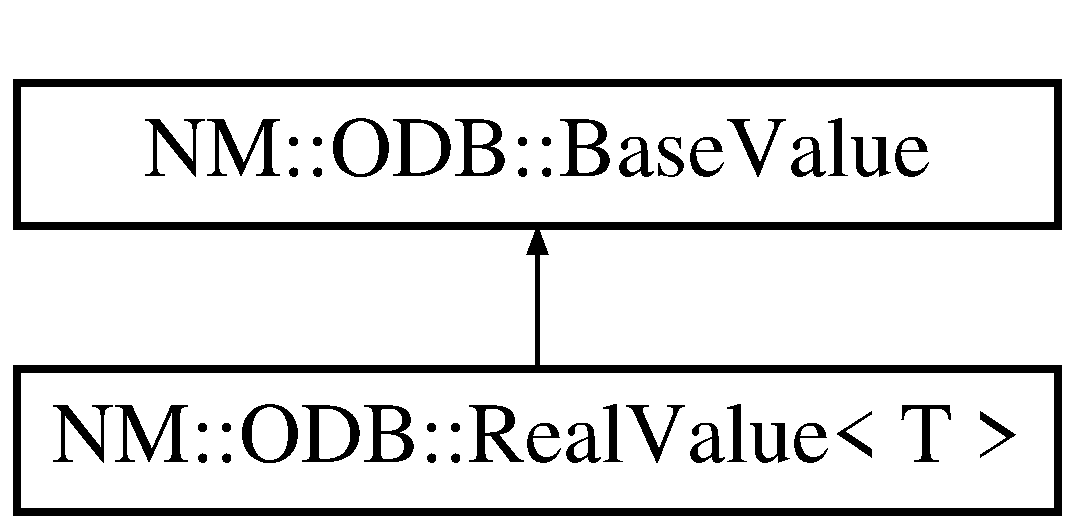
\includegraphics[height=2.000000cm]{class_n_m_1_1_o_d_b_1_1_real_value}
\end{center}
\end{figure}
\subsection*{Public Member Functions}
\begin{DoxyCompactItemize}
\item 
\hyperlink{class_n_m_1_1_o_d_b_1_1_real_value_a6461d728d15aed7ea529343546a364d4}{Real\+Value} (T v)
\item 
\hyperlink{class_n_m_1_1_o_d_b_1_1_real_value_abeec86c680999ab208b0cd8772813338}{$\sim$\+Real\+Value} ()
\item 
\hyperlink{class_n_m_1_1_o_d_b_1_1_real_value}{Real\+Value} $\ast$ \hyperlink{class_n_m_1_1_o_d_b_1_1_real_value_aef8e2c45cf4001f5115d24f8beb1f4df}{Clone} () const 
\item 
\hyperlink{class_n_m_1_1_o_d_b_1_1_real_value_ae521a99bc67b860d58c905a02e39895d}{operator T} () const 
\item 
void \hyperlink{class_n_m_1_1_o_d_b_1_1_real_value_a51fcdc7f0511e26b923ccfc47e20cb08}{Set} (\hyperlink{class_n_m_1_1_o_d_b_1_1_value}{Value} const \&v)
\item 
\+::std\+::wstring \hyperlink{class_n_m_1_1_o_d_b_1_1_real_value_ac34574ad4f573ea467b5469403379f14}{Get\+String\+Value} ()
\item 
bool \hyperlink{class_n_m_1_1_o_d_b_1_1_real_value_a296f8da033d8e15c56d666b4df7fe93f}{operator==} (\hyperlink{class_n_m_1_1_o_d_b_1_1_base_value}{Base\+Value} const \&rhs)
\item 
bool \hyperlink{class_n_m_1_1_o_d_b_1_1_real_value_ad517ae8cfd80888a798c17ecee7435fe}{operator$<$} (\hyperlink{class_n_m_1_1_o_d_b_1_1_base_value}{Base\+Value} const \&rhs)
\item 
bool \hyperlink{class_n_m_1_1_o_d_b_1_1_real_value_a4c7dfb8876b4963fc61104fc19de7b28}{operator$>$} (\hyperlink{class_n_m_1_1_o_d_b_1_1_base_value}{Base\+Value} const \&rhs)
\end{DoxyCompactItemize}
\subsection*{Additional Inherited Members}


\subsection{Detailed Description}
\subsubsection*{template$<$typename T$>$class N\+M\+::\+O\+D\+B\+::\+Real\+Value$<$ T $>$}

Class \hyperlink{class_n_m_1_1_o_d_b_1_1_real_value}{Real\+Value}

The \hyperlink{class_n_m_1_1_o_d_b_1_1_real_value}{Real\+Value} class actually holds the assigned value; Has no direct relationship to \hyperlink{class_n_m_1_1_o_d_b_1_1_attribute}{Attribute} (or visa versa) other than mapped (linked) in each C\+Graph\+Object(\+Vertex, Edge, etc) class \hyperlink{class_n_m_1_1_o_d_b_1_1_attribute}{Attribute}$<$-\/$>$\hyperlink{class_n_m_1_1_o_d_b_1_1_value}{Value} \hyperlink{class_n_m_1_1_o_d_b_1_1_value}{Value} holds a pointer to \hyperlink{class_n_m_1_1_o_d_b_1_1_base_value}{Base\+Value} abstract class of which \hyperlink{class_n_m_1_1_o_d_b_1_1_real_value}{Real\+Value} is the concrete class holding the T datatype and actual assigned value 

\subsection{Constructor \& Destructor Documentation}
\hypertarget{class_n_m_1_1_o_d_b_1_1_real_value_a6461d728d15aed7ea529343546a364d4}{}\index{N\+M\+::\+O\+D\+B\+::\+Real\+Value@{N\+M\+::\+O\+D\+B\+::\+Real\+Value}!Real\+Value@{Real\+Value}}
\index{Real\+Value@{Real\+Value}!N\+M\+::\+O\+D\+B\+::\+Real\+Value@{N\+M\+::\+O\+D\+B\+::\+Real\+Value}}
\subsubsection[{Real\+Value(\+T v)}]{\setlength{\rightskip}{0pt plus 5cm}template$<$typename T$>$ {\bf N\+M\+::\+O\+D\+B\+::\+Real\+Value}$<$ T $>$\+::{\bf Real\+Value} (
\begin{DoxyParamCaption}
\item[{T}]{v}
\end{DoxyParamCaption}
)\hspace{0.3cm}{\ttfamily [inline]}}\label{class_n_m_1_1_o_d_b_1_1_real_value_a6461d728d15aed7ea529343546a364d4}
\hypertarget{class_n_m_1_1_o_d_b_1_1_real_value_abeec86c680999ab208b0cd8772813338}{}\index{N\+M\+::\+O\+D\+B\+::\+Real\+Value@{N\+M\+::\+O\+D\+B\+::\+Real\+Value}!````~Real\+Value@{$\sim$\+Real\+Value}}
\index{````~Real\+Value@{$\sim$\+Real\+Value}!N\+M\+::\+O\+D\+B\+::\+Real\+Value@{N\+M\+::\+O\+D\+B\+::\+Real\+Value}}
\subsubsection[{$\sim$\+Real\+Value()}]{\setlength{\rightskip}{0pt plus 5cm}template$<$typename T$>$ {\bf N\+M\+::\+O\+D\+B\+::\+Real\+Value}$<$ T $>$\+::$\sim${\bf Real\+Value} (
\begin{DoxyParamCaption}
{}
\end{DoxyParamCaption}
)\hspace{0.3cm}{\ttfamily [inline]}}\label{class_n_m_1_1_o_d_b_1_1_real_value_abeec86c680999ab208b0cd8772813338}


\subsection{Member Function Documentation}
\hypertarget{class_n_m_1_1_o_d_b_1_1_real_value_aef8e2c45cf4001f5115d24f8beb1f4df}{}\index{N\+M\+::\+O\+D\+B\+::\+Real\+Value@{N\+M\+::\+O\+D\+B\+::\+Real\+Value}!Clone@{Clone}}
\index{Clone@{Clone}!N\+M\+::\+O\+D\+B\+::\+Real\+Value@{N\+M\+::\+O\+D\+B\+::\+Real\+Value}}
\subsubsection[{Clone() const }]{\setlength{\rightskip}{0pt plus 5cm}template$<$typename T$>$ {\bf Real\+Value}$\ast$ {\bf N\+M\+::\+O\+D\+B\+::\+Real\+Value}$<$ T $>$\+::Clone (
\begin{DoxyParamCaption}
{}
\end{DoxyParamCaption}
) const\hspace{0.3cm}{\ttfamily [inline]}, {\ttfamily [virtual]}}\label{class_n_m_1_1_o_d_b_1_1_real_value_aef8e2c45cf4001f5115d24f8beb1f4df}


Implements \hyperlink{class_n_m_1_1_o_d_b_1_1_base_value_a6e8d5f0d19f1be681fcf582e98cfdfa9}{N\+M\+::\+O\+D\+B\+::\+Base\+Value}.

\hypertarget{class_n_m_1_1_o_d_b_1_1_real_value_ac34574ad4f573ea467b5469403379f14}{}\index{N\+M\+::\+O\+D\+B\+::\+Real\+Value@{N\+M\+::\+O\+D\+B\+::\+Real\+Value}!Get\+String\+Value@{Get\+String\+Value}}
\index{Get\+String\+Value@{Get\+String\+Value}!N\+M\+::\+O\+D\+B\+::\+Real\+Value@{N\+M\+::\+O\+D\+B\+::\+Real\+Value}}
\subsubsection[{Get\+String\+Value()}]{\setlength{\rightskip}{0pt plus 5cm}template$<$typename T$>$ \+::std\+::wstring {\bf N\+M\+::\+O\+D\+B\+::\+Real\+Value}$<$ T $>$\+::Get\+String\+Value (
\begin{DoxyParamCaption}
{}
\end{DoxyParamCaption}
)\hspace{0.3cm}{\ttfamily [inline]}, {\ttfamily [virtual]}}\label{class_n_m_1_1_o_d_b_1_1_real_value_ac34574ad4f573ea467b5469403379f14}


Implements \hyperlink{class_n_m_1_1_o_d_b_1_1_base_value_a1081e74053801b5c525c169e15f63fd3}{N\+M\+::\+O\+D\+B\+::\+Base\+Value}.

\hypertarget{class_n_m_1_1_o_d_b_1_1_real_value_ae521a99bc67b860d58c905a02e39895d}{}\index{N\+M\+::\+O\+D\+B\+::\+Real\+Value@{N\+M\+::\+O\+D\+B\+::\+Real\+Value}!operator T@{operator T}}
\index{operator T@{operator T}!N\+M\+::\+O\+D\+B\+::\+Real\+Value@{N\+M\+::\+O\+D\+B\+::\+Real\+Value}}
\subsubsection[{operator T() const }]{\setlength{\rightskip}{0pt plus 5cm}template$<$typename T$>$ {\bf N\+M\+::\+O\+D\+B\+::\+Real\+Value}$<$ T $>$\+::operator T (
\begin{DoxyParamCaption}
{}
\end{DoxyParamCaption}
) const\hspace{0.3cm}{\ttfamily [inline]}}\label{class_n_m_1_1_o_d_b_1_1_real_value_ae521a99bc67b860d58c905a02e39895d}
\hypertarget{class_n_m_1_1_o_d_b_1_1_real_value_ad517ae8cfd80888a798c17ecee7435fe}{}\index{N\+M\+::\+O\+D\+B\+::\+Real\+Value@{N\+M\+::\+O\+D\+B\+::\+Real\+Value}!operator$<$@{operator$<$}}
\index{operator$<$@{operator$<$}!N\+M\+::\+O\+D\+B\+::\+Real\+Value@{N\+M\+::\+O\+D\+B\+::\+Real\+Value}}
\subsubsection[{operator$<$(\+Base\+Value const \&rhs)}]{\setlength{\rightskip}{0pt plus 5cm}template$<$typename T$>$ bool {\bf N\+M\+::\+O\+D\+B\+::\+Real\+Value}$<$ T $>$\+::operator$<$ (
\begin{DoxyParamCaption}
\item[{{\bf Base\+Value} const \&}]{rhs}
\end{DoxyParamCaption}
)\hspace{0.3cm}{\ttfamily [inline]}, {\ttfamily [virtual]}}\label{class_n_m_1_1_o_d_b_1_1_real_value_ad517ae8cfd80888a798c17ecee7435fe}


Implements \hyperlink{class_n_m_1_1_o_d_b_1_1_base_value_ad6c041908183a43952a17dda329c372a}{N\+M\+::\+O\+D\+B\+::\+Base\+Value}.

\hypertarget{class_n_m_1_1_o_d_b_1_1_real_value_a296f8da033d8e15c56d666b4df7fe93f}{}\index{N\+M\+::\+O\+D\+B\+::\+Real\+Value@{N\+M\+::\+O\+D\+B\+::\+Real\+Value}!operator==@{operator==}}
\index{operator==@{operator==}!N\+M\+::\+O\+D\+B\+::\+Real\+Value@{N\+M\+::\+O\+D\+B\+::\+Real\+Value}}
\subsubsection[{operator==(\+Base\+Value const \&rhs)}]{\setlength{\rightskip}{0pt plus 5cm}template$<$typename T$>$ bool {\bf N\+M\+::\+O\+D\+B\+::\+Real\+Value}$<$ T $>$\+::operator== (
\begin{DoxyParamCaption}
\item[{{\bf Base\+Value} const \&}]{rhs}
\end{DoxyParamCaption}
)\hspace{0.3cm}{\ttfamily [inline]}, {\ttfamily [virtual]}}\label{class_n_m_1_1_o_d_b_1_1_real_value_a296f8da033d8e15c56d666b4df7fe93f}


Implements \hyperlink{class_n_m_1_1_o_d_b_1_1_base_value_a821b57552a15fd85e67f6d3949f19d4d}{N\+M\+::\+O\+D\+B\+::\+Base\+Value}.

\hypertarget{class_n_m_1_1_o_d_b_1_1_real_value_a4c7dfb8876b4963fc61104fc19de7b28}{}\index{N\+M\+::\+O\+D\+B\+::\+Real\+Value@{N\+M\+::\+O\+D\+B\+::\+Real\+Value}!operator$>$@{operator$>$}}
\index{operator$>$@{operator$>$}!N\+M\+::\+O\+D\+B\+::\+Real\+Value@{N\+M\+::\+O\+D\+B\+::\+Real\+Value}}
\subsubsection[{operator$>$(\+Base\+Value const \&rhs)}]{\setlength{\rightskip}{0pt plus 5cm}template$<$typename T$>$ bool {\bf N\+M\+::\+O\+D\+B\+::\+Real\+Value}$<$ T $>$\+::operator$>$ (
\begin{DoxyParamCaption}
\item[{{\bf Base\+Value} const \&}]{rhs}
\end{DoxyParamCaption}
)\hspace{0.3cm}{\ttfamily [inline]}, {\ttfamily [virtual]}}\label{class_n_m_1_1_o_d_b_1_1_real_value_a4c7dfb8876b4963fc61104fc19de7b28}


Implements \hyperlink{class_n_m_1_1_o_d_b_1_1_base_value_aa36d79ee7fd479c798ea6adfabca0b06}{N\+M\+::\+O\+D\+B\+::\+Base\+Value}.

\hypertarget{class_n_m_1_1_o_d_b_1_1_real_value_a51fcdc7f0511e26b923ccfc47e20cb08}{}\index{N\+M\+::\+O\+D\+B\+::\+Real\+Value@{N\+M\+::\+O\+D\+B\+::\+Real\+Value}!Set@{Set}}
\index{Set@{Set}!N\+M\+::\+O\+D\+B\+::\+Real\+Value@{N\+M\+::\+O\+D\+B\+::\+Real\+Value}}
\subsubsection[{Set(\+Value const \&v)}]{\setlength{\rightskip}{0pt plus 5cm}template$<$typename T$>$ void {\bf N\+M\+::\+O\+D\+B\+::\+Real\+Value}$<$ T $>$\+::Set (
\begin{DoxyParamCaption}
\item[{{\bf Value} const \&}]{v}
\end{DoxyParamCaption}
)\hspace{0.3cm}{\ttfamily [inline]}, {\ttfamily [virtual]}}\label{class_n_m_1_1_o_d_b_1_1_real_value_a51fcdc7f0511e26b923ccfc47e20cb08}


Implements \hyperlink{class_n_m_1_1_o_d_b_1_1_base_value_a343cd72d2116513509db379f6faab465}{N\+M\+::\+O\+D\+B\+::\+Base\+Value}.



The documentation for this class was generated from the following file\+:\begin{DoxyCompactItemize}
\item 
C\+:/\+Users/\+Simon/\+Documents/\+Personal/\+Source Code/\+Projects/\+Network\+Modeller/\+Object\+Database/\+Database\+Core\+Elements/\hyperlink{_real_value_8h}{Real\+Value.\+h}\end{DoxyCompactItemize}

\hypertarget{class_n_m_1_1_o_d_b_1_1_sibling}{}\section{N\+M\+:\+:O\+D\+B\+:\+:Sibling Class Reference}
\label{class_n_m_1_1_o_d_b_1_1_sibling}\index{N\+M\+::\+O\+D\+B\+::\+Sibling@{N\+M\+::\+O\+D\+B\+::\+Sibling}}


{\ttfamily \#include $<$Sibling.\+h$>$}

\subsection*{Public Member Functions}
\begin{DoxyCompactItemize}
\item 
\hyperlink{class_n_m_1_1_o_d_b_1_1_sibling_a8e1dd2129154963690b293a95a4edc8c}{Sibling} (\hyperlink{namespace_n_m_1_1_o_d_b_a74e0c94daaeea6f7e783c03a8c921022}{Vertex\+Type} vertex\+Type, \hyperlink{class_n_m_1_1_o_d_b_1_1_c_object_database}{C\+Object\+Database} $\ast$object\+Database\+Ptr)
\item 
\hyperlink{class_n_m_1_1_o_d_b_1_1_sibling_a58c3098a6404d7579457d7250e5bde17}{$\sim$\+Sibling} (void)
\item 
void \hyperlink{class_n_m_1_1_o_d_b_1_1_sibling_acd3e3b9e232b13b70416cda63e8e2d02}{Add\+Sibling} (\hyperlink{class_n_m_1_1_o_d_b_1_1_c_graph_object}{C\+Graph\+Object} $\ast$graph\+Object)
\item 
void \hyperlink{class_n_m_1_1_o_d_b_1_1_sibling_a672ba157483b838ede7c98b3718ed49d}{Delete\+Sibling} (\hyperlink{class_n_m_1_1_o_d_b_1_1_c_graph_object}{C\+Graph\+Object} $\ast$graph\+Object)
\item 
\hyperlink{namespace_n_m_1_1_o_d_b_a262b64fab56baaa96e18bac4ada88265}{O\+B\+J\+E\+C\+T\+U\+I\+D} \hyperlink{class_n_m_1_1_o_d_b_1_1_sibling_a6810fdb47161d77e2b1945933a40178f}{Get\+Sibling} (\hyperlink{namespace_n_m_1_1_o_d_b_a1b474aa7e937112cda42381969dcb55e}{Sibling\+Position} position)
\end{DoxyCompactItemize}


\subsection{Constructor \& Destructor Documentation}
\hypertarget{class_n_m_1_1_o_d_b_1_1_sibling_a8e1dd2129154963690b293a95a4edc8c}{}\index{N\+M\+::\+O\+D\+B\+::\+Sibling@{N\+M\+::\+O\+D\+B\+::\+Sibling}!Sibling@{Sibling}}
\index{Sibling@{Sibling}!N\+M\+::\+O\+D\+B\+::\+Sibling@{N\+M\+::\+O\+D\+B\+::\+Sibling}}
\subsubsection[{Sibling(\+Vertex\+Type vertex\+Type, C\+Object\+Database $\ast$object\+Database\+Ptr)}]{\setlength{\rightskip}{0pt plus 5cm}N\+M\+::\+O\+D\+B\+::\+Sibling\+::\+Sibling (
\begin{DoxyParamCaption}
\item[{{\bf Vertex\+Type}}]{vertex\+Type, }
\item[{{\bf C\+Object\+Database} $\ast$}]{object\+Database\+Ptr}
\end{DoxyParamCaption}
)\hspace{0.3cm}{\ttfamily [explicit]}}\label{class_n_m_1_1_o_d_b_1_1_sibling_a8e1dd2129154963690b293a95a4edc8c}
\hypertarget{class_n_m_1_1_o_d_b_1_1_sibling_a58c3098a6404d7579457d7250e5bde17}{}\index{N\+M\+::\+O\+D\+B\+::\+Sibling@{N\+M\+::\+O\+D\+B\+::\+Sibling}!````~Sibling@{$\sim$\+Sibling}}
\index{````~Sibling@{$\sim$\+Sibling}!N\+M\+::\+O\+D\+B\+::\+Sibling@{N\+M\+::\+O\+D\+B\+::\+Sibling}}
\subsubsection[{$\sim$\+Sibling(void)}]{\setlength{\rightskip}{0pt plus 5cm}N\+M\+::\+O\+D\+B\+::\+Sibling\+::$\sim$\+Sibling (
\begin{DoxyParamCaption}
\item[{void}]{}
\end{DoxyParamCaption}
)}\label{class_n_m_1_1_o_d_b_1_1_sibling_a58c3098a6404d7579457d7250e5bde17}


\subsection{Member Function Documentation}
\hypertarget{class_n_m_1_1_o_d_b_1_1_sibling_acd3e3b9e232b13b70416cda63e8e2d02}{}\index{N\+M\+::\+O\+D\+B\+::\+Sibling@{N\+M\+::\+O\+D\+B\+::\+Sibling}!Add\+Sibling@{Add\+Sibling}}
\index{Add\+Sibling@{Add\+Sibling}!N\+M\+::\+O\+D\+B\+::\+Sibling@{N\+M\+::\+O\+D\+B\+::\+Sibling}}
\subsubsection[{Add\+Sibling(\+C\+Graph\+Object $\ast$graph\+Object)}]{\setlength{\rightskip}{0pt plus 5cm}void N\+M\+::\+O\+D\+B\+::\+Sibling\+::\+Add\+Sibling (
\begin{DoxyParamCaption}
\item[{{\bf C\+Graph\+Object} $\ast$}]{graph\+Object}
\end{DoxyParamCaption}
)}\label{class_n_m_1_1_o_d_b_1_1_sibling_acd3e3b9e232b13b70416cda63e8e2d02}
Add\+Sibling

Adds a sibling to the end of the chain and updates the nextsibling value of the previous node to point to the new node if this is not the first node. \hypertarget{class_n_m_1_1_o_d_b_1_1_sibling_a672ba157483b838ede7c98b3718ed49d}{}\index{N\+M\+::\+O\+D\+B\+::\+Sibling@{N\+M\+::\+O\+D\+B\+::\+Sibling}!Delete\+Sibling@{Delete\+Sibling}}
\index{Delete\+Sibling@{Delete\+Sibling}!N\+M\+::\+O\+D\+B\+::\+Sibling@{N\+M\+::\+O\+D\+B\+::\+Sibling}}
\subsubsection[{Delete\+Sibling(\+C\+Graph\+Object $\ast$graph\+Object)}]{\setlength{\rightskip}{0pt plus 5cm}void N\+M\+::\+O\+D\+B\+::\+Sibling\+::\+Delete\+Sibling (
\begin{DoxyParamCaption}
\item[{{\bf C\+Graph\+Object} $\ast$}]{graph\+Object}
\end{DoxyParamCaption}
)}\label{class_n_m_1_1_o_d_b_1_1_sibling_a672ba157483b838ede7c98b3718ed49d}
Delete\+Sibling

Updates the previoussibling and nextsibling values of the previous and next nodes of the deleted node. Removes the deleted node from the chain and reconnects the chain where the gap is left from deleting the node \hypertarget{class_n_m_1_1_o_d_b_1_1_sibling_a6810fdb47161d77e2b1945933a40178f}{}\index{N\+M\+::\+O\+D\+B\+::\+Sibling@{N\+M\+::\+O\+D\+B\+::\+Sibling}!Get\+Sibling@{Get\+Sibling}}
\index{Get\+Sibling@{Get\+Sibling}!N\+M\+::\+O\+D\+B\+::\+Sibling@{N\+M\+::\+O\+D\+B\+::\+Sibling}}
\subsubsection[{Get\+Sibling(\+Sibling\+Position position)}]{\setlength{\rightskip}{0pt plus 5cm}{\bf O\+B\+J\+E\+C\+T\+U\+I\+D} N\+M\+::\+O\+D\+B\+::\+Sibling\+::\+Get\+Sibling (
\begin{DoxyParamCaption}
\item[{{\bf Sibling\+Position}}]{position}
\end{DoxyParamCaption}
)}\label{class_n_m_1_1_o_d_b_1_1_sibling_a6810fdb47161d77e2b1945933a40178f}


The documentation for this class was generated from the following files\+:\begin{DoxyCompactItemize}
\item 
C\+:/\+Users/\+Simon/\+Documents/\+Personal/\+Source Code/\+Projects/\+Network\+Modeller/\+Object\+Database/\+Tables/\hyperlink{_sibling_8h}{Sibling.\+h}\item 
C\+:/\+Users/\+Simon/\+Documents/\+Personal/\+Source Code/\+Projects/\+Network\+Modeller/\+Object\+Database/\+Tables/\hyperlink{_sibling_8cpp}{Sibling.\+cpp}\end{DoxyCompactItemize}

\hypertarget{class_n_m_1_1_o_d_b_1_1_table_base}{}\section{N\+M\+:\+:O\+D\+B\+:\+:Table\+Base Class Reference}
\label{class_n_m_1_1_o_d_b_1_1_table_base}\index{N\+M\+::\+O\+D\+B\+::\+Table\+Base@{N\+M\+::\+O\+D\+B\+::\+Table\+Base}}


{\ttfamily \#include $<$Table\+Base.\+h$>$}

Inheritance diagram for N\+M\+:\+:O\+D\+B\+:\+:Table\+Base\+:\begin{figure}[H]
\begin{center}
\leavevmode
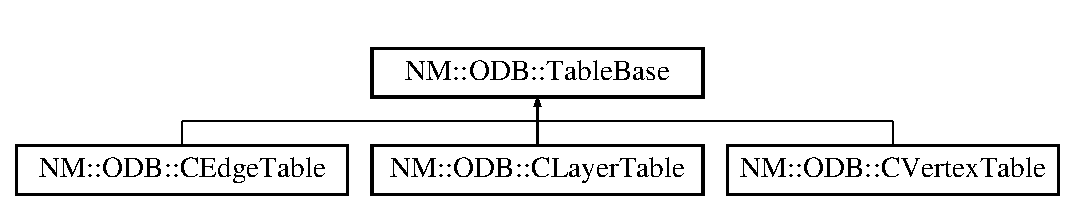
\includegraphics[height=2.000000cm]{class_n_m_1_1_o_d_b_1_1_table_base}
\end{center}
\end{figure}
\subsection*{Public Member Functions}
\begin{DoxyCompactItemize}
\item 
\hyperlink{class_n_m_1_1_o_d_b_1_1_table_base_a14bbb3fa911bf761577ac277cbec2fb3}{Table\+Base} (void)
\item 
\hyperlink{class_n_m_1_1_o_d_b_1_1_table_base_aa87f8c3ccff845bd464f0baa02bb507e}{$\sim$\+Table\+Base} (void)
\item 
virtual bool \hyperlink{class_n_m_1_1_o_d_b_1_1_table_base_afbc340c36e140f2a8184d2585cc3b5d5}{Set\+Value} (\hyperlink{class_n_m_1_1_o_d_b_1_1_c_graph_object}{C\+Graph\+Object} $\ast$, size\+\_\+t idx, \hyperlink{class_n_m_1_1_o_d_b_1_1_value}{Value} const \&v)=0
\item 
virtual bool \hyperlink{class_n_m_1_1_o_d_b_1_1_table_base_a3e55bfe64ccdf81e6a96941b3f9a5fb4}{Set\+Value} (\hyperlink{class_n_m_1_1_o_d_b_1_1_c_graph_object}{C\+Graph\+Object} $\ast$, const \+::std\+::wstring \&attrname, \hyperlink{class_n_m_1_1_o_d_b_1_1_value}{Value} const \&v)=0
\end{DoxyCompactItemize}


\subsection{Constructor \& Destructor Documentation}
\hypertarget{class_n_m_1_1_o_d_b_1_1_table_base_a14bbb3fa911bf761577ac277cbec2fb3}{}\index{N\+M\+::\+O\+D\+B\+::\+Table\+Base@{N\+M\+::\+O\+D\+B\+::\+Table\+Base}!Table\+Base@{Table\+Base}}
\index{Table\+Base@{Table\+Base}!N\+M\+::\+O\+D\+B\+::\+Table\+Base@{N\+M\+::\+O\+D\+B\+::\+Table\+Base}}
\subsubsection[{Table\+Base(void)}]{\setlength{\rightskip}{0pt plus 5cm}N\+M\+::\+O\+D\+B\+::\+Table\+Base\+::\+Table\+Base (
\begin{DoxyParamCaption}
\item[{void}]{}
\end{DoxyParamCaption}
)}\label{class_n_m_1_1_o_d_b_1_1_table_base_a14bbb3fa911bf761577ac277cbec2fb3}
\hypertarget{class_n_m_1_1_o_d_b_1_1_table_base_aa87f8c3ccff845bd464f0baa02bb507e}{}\index{N\+M\+::\+O\+D\+B\+::\+Table\+Base@{N\+M\+::\+O\+D\+B\+::\+Table\+Base}!````~Table\+Base@{$\sim$\+Table\+Base}}
\index{````~Table\+Base@{$\sim$\+Table\+Base}!N\+M\+::\+O\+D\+B\+::\+Table\+Base@{N\+M\+::\+O\+D\+B\+::\+Table\+Base}}
\subsubsection[{$\sim$\+Table\+Base(void)}]{\setlength{\rightskip}{0pt plus 5cm}N\+M\+::\+O\+D\+B\+::\+Table\+Base\+::$\sim$\+Table\+Base (
\begin{DoxyParamCaption}
\item[{void}]{}
\end{DoxyParamCaption}
)}\label{class_n_m_1_1_o_d_b_1_1_table_base_aa87f8c3ccff845bd464f0baa02bb507e}


\subsection{Member Function Documentation}
\hypertarget{class_n_m_1_1_o_d_b_1_1_table_base_afbc340c36e140f2a8184d2585cc3b5d5}{}\index{N\+M\+::\+O\+D\+B\+::\+Table\+Base@{N\+M\+::\+O\+D\+B\+::\+Table\+Base}!Set\+Value@{Set\+Value}}
\index{Set\+Value@{Set\+Value}!N\+M\+::\+O\+D\+B\+::\+Table\+Base@{N\+M\+::\+O\+D\+B\+::\+Table\+Base}}
\subsubsection[{Set\+Value(\+C\+Graph\+Object $\ast$, size\+\_\+t idx, Value const \&v)=0}]{\setlength{\rightskip}{0pt plus 5cm}virtual bool N\+M\+::\+O\+D\+B\+::\+Table\+Base\+::\+Set\+Value (
\begin{DoxyParamCaption}
\item[{{\bf C\+Graph\+Object} $\ast$}]{, }
\item[{size\+\_\+t}]{idx, }
\item[{{\bf Value} const \&}]{v}
\end{DoxyParamCaption}
)\hspace{0.3cm}{\ttfamily [pure virtual]}}\label{class_n_m_1_1_o_d_b_1_1_table_base_afbc340c36e140f2a8184d2585cc3b5d5}


Implemented in \hyperlink{class_n_m_1_1_o_d_b_1_1_c_vertex_table_ad6c21c25a002804c3255771d15a513bf}{N\+M\+::\+O\+D\+B\+::\+C\+Vertex\+Table}, \hyperlink{class_n_m_1_1_o_d_b_1_1_c_layer_table_a71a6bb2dbac48f3dd636c25d7d1b31f0}{N\+M\+::\+O\+D\+B\+::\+C\+Layer\+Table}, and \hyperlink{class_n_m_1_1_o_d_b_1_1_c_edge_table_a67f722668bfebd46ac05288e20523003}{N\+M\+::\+O\+D\+B\+::\+C\+Edge\+Table}.

\hypertarget{class_n_m_1_1_o_d_b_1_1_table_base_a3e55bfe64ccdf81e6a96941b3f9a5fb4}{}\index{N\+M\+::\+O\+D\+B\+::\+Table\+Base@{N\+M\+::\+O\+D\+B\+::\+Table\+Base}!Set\+Value@{Set\+Value}}
\index{Set\+Value@{Set\+Value}!N\+M\+::\+O\+D\+B\+::\+Table\+Base@{N\+M\+::\+O\+D\+B\+::\+Table\+Base}}
\subsubsection[{Set\+Value(\+C\+Graph\+Object $\ast$, const \+::std\+::wstring \&attrname, Value const \&v)=0}]{\setlength{\rightskip}{0pt plus 5cm}virtual bool N\+M\+::\+O\+D\+B\+::\+Table\+Base\+::\+Set\+Value (
\begin{DoxyParamCaption}
\item[{{\bf C\+Graph\+Object} $\ast$}]{, }
\item[{const \+::std\+::wstring \&}]{attrname, }
\item[{{\bf Value} const \&}]{v}
\end{DoxyParamCaption}
)\hspace{0.3cm}{\ttfamily [pure virtual]}}\label{class_n_m_1_1_o_d_b_1_1_table_base_a3e55bfe64ccdf81e6a96941b3f9a5fb4}


Implemented in \hyperlink{class_n_m_1_1_o_d_b_1_1_c_vertex_table_a1433c9bce4a02925cf39e0d13ed4d19b}{N\+M\+::\+O\+D\+B\+::\+C\+Vertex\+Table}, \hyperlink{class_n_m_1_1_o_d_b_1_1_c_layer_table_a589923308ca7e92665b9999572d36bbd}{N\+M\+::\+O\+D\+B\+::\+C\+Layer\+Table}, and \hyperlink{class_n_m_1_1_o_d_b_1_1_c_edge_table_ad210f2bbf1ba2c9e3a314814a8c1df9e}{N\+M\+::\+O\+D\+B\+::\+C\+Edge\+Table}.



The documentation for this class was generated from the following files\+:\begin{DoxyCompactItemize}
\item 
C\+:/\+Users/\+Simon/\+Documents/\+Personal/\+Source Code/\+Projects/\+Network\+Modeller/\+Object\+Database/\+Tables/\hyperlink{_table_base_8h}{Table\+Base.\+h}\item 
C\+:/\+Users/\+Simon/\+Documents/\+Personal/\+Source Code/\+Projects/\+Network\+Modeller/\+Object\+Database/\+Tables/\hyperlink{_table_base_8cpp}{Table\+Base.\+cpp}\end{DoxyCompactItemize}

\hypertarget{class_n_m_1_1_o_d_b_1_1_value}{}\section{N\+M\+:\+:O\+D\+B\+:\+:Value Class Reference}
\label{class_n_m_1_1_o_d_b_1_1_value}\index{N\+M\+::\+O\+D\+B\+::\+Value@{N\+M\+::\+O\+D\+B\+::\+Value}}


{\ttfamily \#include $<$Value.\+h$>$}

\subsection*{Public Member Functions}
\begin{DoxyCompactItemize}
\item 
\hyperlink{class_n_m_1_1_o_d_b_1_1_value_aff9458b1709a5a8e4cb533009a60c872}{Value} (\hyperlink{class_n_m_1_1_o_d_b_1_1_base_value}{Base\+Value} const \&bv)
\item 
\hyperlink{class_n_m_1_1_o_d_b_1_1_value_af54d981ec82cdf060be9e2bf09895c4c}{Value} (const \hyperlink{class_n_m_1_1_o_d_b_1_1_value}{Value} \&rhs)
\item 
\hyperlink{class_n_m_1_1_o_d_b_1_1_value}{Value} \& \hyperlink{class_n_m_1_1_o_d_b_1_1_value_a230d165d17cb0a6d7f658f052eef4b2c}{operator=} (const \hyperlink{class_n_m_1_1_o_d_b_1_1_value}{Value} \&rhs)
\item 
\hyperlink{class_n_m_1_1_o_d_b_1_1_value_a89465dc415cf1e79bdfb661aa038eda0}{$\sim$\+Value} ()
\item 
{\footnotesize template$<$typename T $>$ }\\T \hyperlink{class_n_m_1_1_o_d_b_1_1_value_a274f294d919e7baba602d42d65c1e3a8}{Get} () const 
\item 
bool \hyperlink{class_n_m_1_1_o_d_b_1_1_value_a3c8038dd797e998e49931ea25ee5a1d2}{operator==} (const \hyperlink{class_n_m_1_1_o_d_b_1_1_value}{Value} \&rhs)
\item 
bool \hyperlink{class_n_m_1_1_o_d_b_1_1_value_ad4017a9ca04a72d93963c3a2d030c1da}{operator$<$} (const \hyperlink{class_n_m_1_1_o_d_b_1_1_value}{Value} \&rhs)
\item 
bool \hyperlink{class_n_m_1_1_o_d_b_1_1_value_aa73e9b2f51907a0ce259bf35cc677479}{operator$>$} (const \hyperlink{class_n_m_1_1_o_d_b_1_1_value}{Value} \&rhs)
\end{DoxyCompactItemize}


\subsection{Constructor \& Destructor Documentation}
\hypertarget{class_n_m_1_1_o_d_b_1_1_value_aff9458b1709a5a8e4cb533009a60c872}{}\index{N\+M\+::\+O\+D\+B\+::\+Value@{N\+M\+::\+O\+D\+B\+::\+Value}!Value@{Value}}
\index{Value@{Value}!N\+M\+::\+O\+D\+B\+::\+Value@{N\+M\+::\+O\+D\+B\+::\+Value}}
\subsubsection[{Value(\+Base\+Value const \&bv)}]{\setlength{\rightskip}{0pt plus 5cm}N\+M\+::\+O\+D\+B\+::\+Value\+::\+Value (
\begin{DoxyParamCaption}
\item[{{\bf Base\+Value} const \&}]{bv}
\end{DoxyParamCaption}
)}\label{class_n_m_1_1_o_d_b_1_1_value_aff9458b1709a5a8e4cb533009a60c872}
\hypertarget{class_n_m_1_1_o_d_b_1_1_value_af54d981ec82cdf060be9e2bf09895c4c}{}\index{N\+M\+::\+O\+D\+B\+::\+Value@{N\+M\+::\+O\+D\+B\+::\+Value}!Value@{Value}}
\index{Value@{Value}!N\+M\+::\+O\+D\+B\+::\+Value@{N\+M\+::\+O\+D\+B\+::\+Value}}
\subsubsection[{Value(const Value \&rhs)}]{\setlength{\rightskip}{0pt plus 5cm}N\+M\+::\+O\+D\+B\+::\+Value\+::\+Value (
\begin{DoxyParamCaption}
\item[{const {\bf Value} \&}]{rhs}
\end{DoxyParamCaption}
)}\label{class_n_m_1_1_o_d_b_1_1_value_af54d981ec82cdf060be9e2bf09895c4c}
\hypertarget{class_n_m_1_1_o_d_b_1_1_value_a89465dc415cf1e79bdfb661aa038eda0}{}\index{N\+M\+::\+O\+D\+B\+::\+Value@{N\+M\+::\+O\+D\+B\+::\+Value}!````~Value@{$\sim$\+Value}}
\index{````~Value@{$\sim$\+Value}!N\+M\+::\+O\+D\+B\+::\+Value@{N\+M\+::\+O\+D\+B\+::\+Value}}
\subsubsection[{$\sim$\+Value()}]{\setlength{\rightskip}{0pt plus 5cm}N\+M\+::\+O\+D\+B\+::\+Value\+::$\sim$\+Value (
\begin{DoxyParamCaption}
{}
\end{DoxyParamCaption}
)}\label{class_n_m_1_1_o_d_b_1_1_value_a89465dc415cf1e79bdfb661aa038eda0}


\subsection{Member Function Documentation}
\hypertarget{class_n_m_1_1_o_d_b_1_1_value_a274f294d919e7baba602d42d65c1e3a8}{}\index{N\+M\+::\+O\+D\+B\+::\+Value@{N\+M\+::\+O\+D\+B\+::\+Value}!Get@{Get}}
\index{Get@{Get}!N\+M\+::\+O\+D\+B\+::\+Value@{N\+M\+::\+O\+D\+B\+::\+Value}}
\subsubsection[{Get() const }]{\setlength{\rightskip}{0pt plus 5cm}template$<$typename T $>$ T N\+M\+::\+O\+D\+B\+::\+Value\+::\+Get (
\begin{DoxyParamCaption}
{}
\end{DoxyParamCaption}
) const\hspace{0.3cm}{\ttfamily [inline]}}\label{class_n_m_1_1_o_d_b_1_1_value_a274f294d919e7baba602d42d65c1e3a8}
Get \hyperlink{class_n_m_1_1_o_d_b_1_1_value}{Value} by type

Returns the value as its native type i.\+e. int, double, float etc

moved out of \hyperlink{_value_8cpp}{Value.\+cpp} due to linker errors \hypertarget{class_n_m_1_1_o_d_b_1_1_value_ad4017a9ca04a72d93963c3a2d030c1da}{}\index{N\+M\+::\+O\+D\+B\+::\+Value@{N\+M\+::\+O\+D\+B\+::\+Value}!operator$<$@{operator$<$}}
\index{operator$<$@{operator$<$}!N\+M\+::\+O\+D\+B\+::\+Value@{N\+M\+::\+O\+D\+B\+::\+Value}}
\subsubsection[{operator$<$(const Value \&rhs)}]{\setlength{\rightskip}{0pt plus 5cm}bool N\+M\+::\+O\+D\+B\+::\+Value\+::operator$<$ (
\begin{DoxyParamCaption}
\item[{const {\bf Value} \&}]{rhs}
\end{DoxyParamCaption}
)}\label{class_n_m_1_1_o_d_b_1_1_value_ad4017a9ca04a72d93963c3a2d030c1da}
\hypertarget{class_n_m_1_1_o_d_b_1_1_value_a230d165d17cb0a6d7f658f052eef4b2c}{}\index{N\+M\+::\+O\+D\+B\+::\+Value@{N\+M\+::\+O\+D\+B\+::\+Value}!operator=@{operator=}}
\index{operator=@{operator=}!N\+M\+::\+O\+D\+B\+::\+Value@{N\+M\+::\+O\+D\+B\+::\+Value}}
\subsubsection[{operator=(const Value \&rhs)}]{\setlength{\rightskip}{0pt plus 5cm}{\bf Value} \& N\+M\+::\+O\+D\+B\+::\+Value\+::operator= (
\begin{DoxyParamCaption}
\item[{const {\bf Value} \&}]{rhs}
\end{DoxyParamCaption}
)}\label{class_n_m_1_1_o_d_b_1_1_value_a230d165d17cb0a6d7f658f052eef4b2c}
\hypertarget{class_n_m_1_1_o_d_b_1_1_value_a3c8038dd797e998e49931ea25ee5a1d2}{}\index{N\+M\+::\+O\+D\+B\+::\+Value@{N\+M\+::\+O\+D\+B\+::\+Value}!operator==@{operator==}}
\index{operator==@{operator==}!N\+M\+::\+O\+D\+B\+::\+Value@{N\+M\+::\+O\+D\+B\+::\+Value}}
\subsubsection[{operator==(const Value \&rhs)}]{\setlength{\rightskip}{0pt plus 5cm}bool N\+M\+::\+O\+D\+B\+::\+Value\+::operator== (
\begin{DoxyParamCaption}
\item[{const {\bf Value} \&}]{rhs}
\end{DoxyParamCaption}
)}\label{class_n_m_1_1_o_d_b_1_1_value_a3c8038dd797e998e49931ea25ee5a1d2}
\hypertarget{class_n_m_1_1_o_d_b_1_1_value_aa73e9b2f51907a0ce259bf35cc677479}{}\index{N\+M\+::\+O\+D\+B\+::\+Value@{N\+M\+::\+O\+D\+B\+::\+Value}!operator$>$@{operator$>$}}
\index{operator$>$@{operator$>$}!N\+M\+::\+O\+D\+B\+::\+Value@{N\+M\+::\+O\+D\+B\+::\+Value}}
\subsubsection[{operator$>$(const Value \&rhs)}]{\setlength{\rightskip}{0pt plus 5cm}bool N\+M\+::\+O\+D\+B\+::\+Value\+::operator$>$ (
\begin{DoxyParamCaption}
\item[{const {\bf Value} \&}]{rhs}
\end{DoxyParamCaption}
)}\label{class_n_m_1_1_o_d_b_1_1_value_aa73e9b2f51907a0ce259bf35cc677479}


The documentation for this class was generated from the following files\+:\begin{DoxyCompactItemize}
\item 
C\+:/\+Users/\+Simon/\+Documents/\+Personal/\+Source Code/\+Projects/\+Network\+Modeller/\+Object\+Database/\+Database\+Core\+Elements/\hyperlink{_value_8h}{Value.\+h}\item 
C\+:/\+Users/\+Simon/\+Documents/\+Personal/\+Source Code/\+Projects/\+Network\+Modeller/\+Object\+Database/\+Database\+Core\+Elements/\hyperlink{_value_8cpp}{Value.\+cpp}\end{DoxyCompactItemize}

\chapter{File Documentation}
\hypertarget{attribute_8cpp}{}\section{C\+:/\+Users/\+Simon/\+Documents/\+Personal/\+Source Code/\+Projects/\+Network\+Modeller/\+Object\+Database/\+Database\+Core\+Elements/attribute.cpp File Reference}
\label{attribute_8cpp}\index{C\+:/\+Users/\+Simon/\+Documents/\+Personal/\+Source Code/\+Projects/\+Network\+Modeller/\+Object\+Database/\+Database\+Core\+Elements/attribute.\+cpp@{C\+:/\+Users/\+Simon/\+Documents/\+Personal/\+Source Code/\+Projects/\+Network\+Modeller/\+Object\+Database/\+Database\+Core\+Elements/attribute.\+cpp}}
{\ttfamily \#include \char`\"{}stdafx.\+h\char`\"{}}\\*
{\ttfamily \#include \char`\"{}Attribute.\+h\char`\"{}}\\*

\hypertarget{attribute_8h}{}\section{C\+:/\+Users/\+Simon/\+Documents/\+Personal/\+Source Code/\+Projects/\+Network\+Modeller/\+Object\+Database/\+Database\+Core\+Elements/attribute.h File Reference}
\label{attribute_8h}\index{C\+:/\+Users/\+Simon/\+Documents/\+Personal/\+Source Code/\+Projects/\+Network\+Modeller/\+Object\+Database/\+Database\+Core\+Elements/attribute.\+h@{C\+:/\+Users/\+Simon/\+Documents/\+Personal/\+Source Code/\+Projects/\+Network\+Modeller/\+Object\+Database/\+Database\+Core\+Elements/attribute.\+h}}
{\ttfamily \#include $<$string$>$}\\*
{\ttfamily \#include \char`\"{}Value.\+h\char`\"{}}\\*
{\ttfamily \#include \char`\"{}Type.\+h\char`\"{}}\\*
\subsection*{Classes}
\begin{DoxyCompactItemize}
\item 
class \hyperlink{class_n_m_1_1_o_d_b_1_1_attribute}{N\+M\+::\+O\+D\+B\+::\+Attribute}
\end{DoxyCompactItemize}
\subsection*{Namespaces}
\begin{DoxyCompactItemize}
\item 
 \hyperlink{namespace_n_m}{N\+M}
\item 
 \hyperlink{namespace_n_m_1_1_o_d_b}{N\+M\+::\+O\+D\+B}
\end{DoxyCompactItemize}

\hypertarget{_base_value_8h}{}\section{C\+:/\+Users/\+Simon/\+Documents/\+Personal/\+Source Code/\+Projects/\+Network\+Modeller/\+Object\+Database/\+Database\+Core\+Elements/\+Base\+Value.h File Reference}
\label{_base_value_8h}\index{C\+:/\+Users/\+Simon/\+Documents/\+Personal/\+Source Code/\+Projects/\+Network\+Modeller/\+Object\+Database/\+Database\+Core\+Elements/\+Base\+Value.\+h@{C\+:/\+Users/\+Simon/\+Documents/\+Personal/\+Source Code/\+Projects/\+Network\+Modeller/\+Object\+Database/\+Database\+Core\+Elements/\+Base\+Value.\+h}}
{\ttfamily \#include $<$string$>$}\\*
\subsection*{Classes}
\begin{DoxyCompactItemize}
\item 
class \hyperlink{class_n_m_1_1_o_d_b_1_1_base_value}{N\+M\+::\+O\+D\+B\+::\+Base\+Value}
\end{DoxyCompactItemize}
\subsection*{Namespaces}
\begin{DoxyCompactItemize}
\item 
 \hyperlink{namespace_n_m}{N\+M}
\item 
 \hyperlink{namespace_n_m_1_1_o_d_b}{N\+M\+::\+O\+D\+B}
\end{DoxyCompactItemize}

\hypertarget{_graph_object_database_8cpp}{}\section{C\+:/\+Users/\+Simon/\+Documents/\+Personal/\+Source Code/\+Projects/\+Network\+Modeller/\+Object\+Database/\+Database\+Core\+Elements/\+Graph\+Object\+Database.cpp File Reference}
\label{_graph_object_database_8cpp}\index{C\+:/\+Users/\+Simon/\+Documents/\+Personal/\+Source Code/\+Projects/\+Network\+Modeller/\+Object\+Database/\+Database\+Core\+Elements/\+Graph\+Object\+Database.\+cpp@{C\+:/\+Users/\+Simon/\+Documents/\+Personal/\+Source Code/\+Projects/\+Network\+Modeller/\+Object\+Database/\+Database\+Core\+Elements/\+Graph\+Object\+Database.\+cpp}}
{\ttfamily \#include \char`\"{}stdafx.\+h\char`\"{}}\\*
{\ttfamily \#include \char`\"{}Graph\+Object\+Database.\+h\char`\"{}}\\*
{\ttfamily \#include \char`\"{}C\+Type.\+h\char`\"{}}\\*
{\ttfamily \#include $<$vector$>$}\\*
\subsection*{Namespaces}
\begin{DoxyCompactItemize}
\item 
 \hyperlink{namespace_n_m}{N\+M}
\item 
 \hyperlink{namespace_n_m_1_1_o_d_b}{N\+M\+::\+O\+D\+B}
\end{DoxyCompactItemize}

\hypertarget{_graph_object_database_8h}{}\section{C\+:/\+Users/\+Simon/\+Documents/\+Personal/\+Source Code/\+Projects/\+Network\+Modeller/\+Object\+Database/\+Database\+Core\+Elements/\+Graph\+Object\+Database.h File Reference}
\label{_graph_object_database_8h}\index{C\+:/\+Users/\+Simon/\+Documents/\+Personal/\+Source Code/\+Projects/\+Network\+Modeller/\+Object\+Database/\+Database\+Core\+Elements/\+Graph\+Object\+Database.\+h@{C\+:/\+Users/\+Simon/\+Documents/\+Personal/\+Source Code/\+Projects/\+Network\+Modeller/\+Object\+Database/\+Database\+Core\+Elements/\+Graph\+Object\+Database.\+h}}
{\ttfamily \#include \char`\"{}Base\+Value.\+h\char`\"{}}\\*
{\ttfamily \#include \char`\"{}Value.\+h\char`\"{}}\\*
{\ttfamily \#include \char`\"{}Real\+Value.\+h\char`\"{}}\\*
{\ttfamily \#include \char`\"{}Type.\+h\char`\"{}}\\*
{\ttfamily \#include \char`\"{}Attribute.\+h\char`\"{}}\\*

\hypertarget{_real_value_8cpp}{}\section{C\+:/\+Users/\+Simon/\+Documents/\+Personal/\+Source Code/\+Projects/\+Network\+Modeller/\+Object\+Database/\+Database\+Core\+Elements/\+Real\+Value.cpp File Reference}
\label{_real_value_8cpp}\index{C\+:/\+Users/\+Simon/\+Documents/\+Personal/\+Source Code/\+Projects/\+Network\+Modeller/\+Object\+Database/\+Database\+Core\+Elements/\+Real\+Value.\+cpp@{C\+:/\+Users/\+Simon/\+Documents/\+Personal/\+Source Code/\+Projects/\+Network\+Modeller/\+Object\+Database/\+Database\+Core\+Elements/\+Real\+Value.\+cpp}}

\hypertarget{_real_value_8h}{}\section{C\+:/\+Users/\+Simon/\+Documents/\+Personal/\+Source Code/\+Projects/\+Network\+Modeller/\+Object\+Database/\+Database\+Core\+Elements/\+Real\+Value.h File Reference}
\label{_real_value_8h}\index{C\+:/\+Users/\+Simon/\+Documents/\+Personal/\+Source Code/\+Projects/\+Network\+Modeller/\+Object\+Database/\+Database\+Core\+Elements/\+Real\+Value.\+h@{C\+:/\+Users/\+Simon/\+Documents/\+Personal/\+Source Code/\+Projects/\+Network\+Modeller/\+Object\+Database/\+Database\+Core\+Elements/\+Real\+Value.\+h}}
{\ttfamily \#include \char`\"{}Base\+Value.\+h\char`\"{}}\\*
\subsection*{Classes}
\begin{DoxyCompactItemize}
\item 
class \hyperlink{class_n_m_1_1_o_d_b_1_1_real_value}{N\+M\+::\+O\+D\+B\+::\+Real\+Value$<$ T $>$}
\end{DoxyCompactItemize}
\subsection*{Namespaces}
\begin{DoxyCompactItemize}
\item 
 \hyperlink{namespace_n_m}{N\+M}
\item 
 \hyperlink{namespace_n_m_1_1_o_d_b}{N\+M\+::\+O\+D\+B}
\end{DoxyCompactItemize}

\hypertarget{_type_8h}{}\section{C\+:/\+Users/\+Simon/\+Documents/\+Personal/\+Source Code/\+Projects/\+Network\+Modeller/\+Object\+Database/\+Database\+Core\+Elements/\+Type.h File Reference}
\label{_type_8h}\index{C\+:/\+Users/\+Simon/\+Documents/\+Personal/\+Source Code/\+Projects/\+Network\+Modeller/\+Object\+Database/\+Database\+Core\+Elements/\+Type.\+h@{C\+:/\+Users/\+Simon/\+Documents/\+Personal/\+Source Code/\+Projects/\+Network\+Modeller/\+Object\+Database/\+Database\+Core\+Elements/\+Type.\+h}}
{\ttfamily \#include $<$vector$>$}\\*
{\ttfamily \#include \char`\"{}Real\+Value.\+h\char`\"{}}\\*
{\ttfamily \#include \char`\"{}..\textbackslash{}\+Interfaces\textbackslash{}\+Object\+Database\+Defines.\+h\char`\"{}}\\*
\subsection*{Classes}
\begin{DoxyCompactItemize}
\item 
class \hyperlink{class_n_m_1_1_o_d_b_1_1_c_type}{N\+M\+::\+O\+D\+B\+::\+C\+Type}
\end{DoxyCompactItemize}
\subsection*{Namespaces}
\begin{DoxyCompactItemize}
\item 
 \hyperlink{namespace_n_m}{N\+M}
\item 
 \hyperlink{namespace_n_m_1_1_o_d_b}{N\+M\+::\+O\+D\+B}
\end{DoxyCompactItemize}

\hypertarget{_value_8cpp}{}\section{C\+:/\+Users/\+Simon/\+Documents/\+Personal/\+Source Code/\+Projects/\+Network\+Modeller/\+Object\+Database/\+Database\+Core\+Elements/\+Value.cpp File Reference}
\label{_value_8cpp}\index{C\+:/\+Users/\+Simon/\+Documents/\+Personal/\+Source Code/\+Projects/\+Network\+Modeller/\+Object\+Database/\+Database\+Core\+Elements/\+Value.\+cpp@{C\+:/\+Users/\+Simon/\+Documents/\+Personal/\+Source Code/\+Projects/\+Network\+Modeller/\+Object\+Database/\+Database\+Core\+Elements/\+Value.\+cpp}}
{\ttfamily \#include \char`\"{}stdafx.\+h\char`\"{}}\\*
{\ttfamily \#include \char`\"{}Value.\+h\char`\"{}}\\*
{\ttfamily \#include \char`\"{}Graph\+Object\+Database.\+h\char`\"{}}\\*
\subsection*{Namespaces}
\begin{DoxyCompactItemize}
\item 
 \hyperlink{namespace_n_m}{N\+M}
\item 
 \hyperlink{namespace_n_m_1_1_o_d_b}{N\+M\+::\+O\+D\+B}
\end{DoxyCompactItemize}

\hypertarget{_value_8h}{}\section{C\+:/\+Users/\+Simon/\+Documents/\+Personal/\+Source Code/\+Projects/\+Network\+Modeller/\+Object\+Database/\+Database\+Core\+Elements/\+Value.h File Reference}
\label{_value_8h}\index{C\+:/\+Users/\+Simon/\+Documents/\+Personal/\+Source Code/\+Projects/\+Network\+Modeller/\+Object\+Database/\+Database\+Core\+Elements/\+Value.\+h@{C\+:/\+Users/\+Simon/\+Documents/\+Personal/\+Source Code/\+Projects/\+Network\+Modeller/\+Object\+Database/\+Database\+Core\+Elements/\+Value.\+h}}
\subsection*{Classes}
\begin{DoxyCompactItemize}
\item 
class \hyperlink{class_n_m_1_1_o_d_b_1_1_value}{N\+M\+::\+O\+D\+B\+::\+Value}
\end{DoxyCompactItemize}
\subsection*{Namespaces}
\begin{DoxyCompactItemize}
\item 
 \hyperlink{namespace_n_m}{N\+M}
\item 
 \hyperlink{namespace_n_m_1_1_o_d_b}{N\+M\+::\+O\+D\+B}
\end{DoxyCompactItemize}

\hypertarget{_database_observer_8h}{}\section{C\+:/\+Users/\+Simon/\+Documents/\+Personal/\+Source Code/\+Projects/\+Network\+Modeller/\+Object\+Database/\+Database\+Observer.h File Reference}
\label{_database_observer_8h}\index{C\+:/\+Users/\+Simon/\+Documents/\+Personal/\+Source Code/\+Projects/\+Network\+Modeller/\+Object\+Database/\+Database\+Observer.\+h@{C\+:/\+Users/\+Simon/\+Documents/\+Personal/\+Source Code/\+Projects/\+Network\+Modeller/\+Object\+Database/\+Database\+Observer.\+h}}
\subsection*{Classes}
\begin{DoxyCompactItemize}
\item 
class \hyperlink{class_n_m_1_1_o_d_b_1_1_c_database_observer}{N\+M\+::\+O\+D\+B\+::\+C\+Database\+Observer}
\end{DoxyCompactItemize}
\subsection*{Namespaces}
\begin{DoxyCompactItemize}
\item 
 \hyperlink{namespace_n_m}{N\+M}
\item 
 \hyperlink{namespace_n_m_1_1_o_d_b}{N\+M\+::\+O\+D\+B}
\end{DoxyCompactItemize}

\hypertarget{_attribute_update_8cpp}{}\section{C\+:/\+Users/\+Simon/\+Documents/\+Personal/\+Source Code/\+Projects/\+Network\+Modeller/\+Object\+Database/\+Database\+Update\+Elements/\+Attribute\+Update.cpp File Reference}
\label{_attribute_update_8cpp}\index{C\+:/\+Users/\+Simon/\+Documents/\+Personal/\+Source Code/\+Projects/\+Network\+Modeller/\+Object\+Database/\+Database\+Update\+Elements/\+Attribute\+Update.\+cpp@{C\+:/\+Users/\+Simon/\+Documents/\+Personal/\+Source Code/\+Projects/\+Network\+Modeller/\+Object\+Database/\+Database\+Update\+Elements/\+Attribute\+Update.\+cpp}}
{\ttfamily \#include \char`\"{}stdafx.\+h\char`\"{}}\\*
{\ttfamily \#include \char`\"{}Attribute\+Update.\+h\char`\"{}}\\*
\subsection*{Namespaces}
\begin{DoxyCompactItemize}
\item 
 \hyperlink{namespace_n_m}{N\+M}
\item 
 \hyperlink{namespace_n_m_1_1_o_d_b}{N\+M\+::\+O\+D\+B}
\end{DoxyCompactItemize}

\hypertarget{_attribute_update_8h}{}\section{C\+:/\+Users/\+Simon/\+Documents/\+Personal/\+Source Code/\+Projects/\+Network\+Modeller/\+Object\+Database/\+Database\+Update\+Elements/\+Attribute\+Update.h File Reference}
\label{_attribute_update_8h}\index{C\+:/\+Users/\+Simon/\+Documents/\+Personal/\+Source Code/\+Projects/\+Network\+Modeller/\+Object\+Database/\+Database\+Update\+Elements/\+Attribute\+Update.\+h@{C\+:/\+Users/\+Simon/\+Documents/\+Personal/\+Source Code/\+Projects/\+Network\+Modeller/\+Object\+Database/\+Database\+Update\+Elements/\+Attribute\+Update.\+h}}
{\ttfamily \#include \char`\"{}..\textbackslash{}\+Database\+Core\+Elements\textbackslash{}\+Value.\+h\char`\"{}}\\*
\subsection*{Classes}
\begin{DoxyCompactItemize}
\item 
class \hyperlink{class_n_m_1_1_o_d_b_1_1_attribute_update}{N\+M\+::\+O\+D\+B\+::\+Attribute\+Update}
\end{DoxyCompactItemize}
\subsection*{Namespaces}
\begin{DoxyCompactItemize}
\item 
 \hyperlink{namespace_n_m}{N\+M}
\item 
 \hyperlink{namespace_n_m_1_1_o_d_b}{N\+M\+::\+O\+D\+B}
\end{DoxyCompactItemize}

\hypertarget{_database_notification_requests_8cpp}{}\section{C\+:/\+Users/\+Simon/\+Documents/\+Personal/\+Source Code/\+Projects/\+Network\+Modeller/\+Object\+Database/\+Database\+Update\+Elements/\+Database\+Notification\+Requests.cpp File Reference}
\label{_database_notification_requests_8cpp}\index{C\+:/\+Users/\+Simon/\+Documents/\+Personal/\+Source Code/\+Projects/\+Network\+Modeller/\+Object\+Database/\+Database\+Update\+Elements/\+Database\+Notification\+Requests.\+cpp@{C\+:/\+Users/\+Simon/\+Documents/\+Personal/\+Source Code/\+Projects/\+Network\+Modeller/\+Object\+Database/\+Database\+Update\+Elements/\+Database\+Notification\+Requests.\+cpp}}
{\ttfamily \#include \char`\"{}stdafx.\+h\char`\"{}}\\*
{\ttfamily \#include \char`\"{}Database\+Notification\+Requests.\+h\char`\"{}}\\*
{\ttfamily \#include $<$vector$>$}\\*
\subsection*{Namespaces}
\begin{DoxyCompactItemize}
\item 
 \hyperlink{namespace_n_m}{N\+M}
\item 
 \hyperlink{namespace_n_m_1_1_o_d_b}{N\+M\+::\+O\+D\+B}
\end{DoxyCompactItemize}

\hypertarget{_database_notification_requests_8h}{}\section{C\+:/\+Users/\+Simon/\+Documents/\+Personal/\+Source Code/\+Projects/\+Network\+Modeller/\+Object\+Database/\+Database\+Update\+Elements/\+Database\+Notification\+Requests.h File Reference}
\label{_database_notification_requests_8h}\index{C\+:/\+Users/\+Simon/\+Documents/\+Personal/\+Source Code/\+Projects/\+Network\+Modeller/\+Object\+Database/\+Database\+Update\+Elements/\+Database\+Notification\+Requests.\+h@{C\+:/\+Users/\+Simon/\+Documents/\+Personal/\+Source Code/\+Projects/\+Network\+Modeller/\+Object\+Database/\+Database\+Update\+Elements/\+Database\+Notification\+Requests.\+h}}
{\ttfamily \#include \char`\"{}..\textbackslash{}\+Factory\textbackslash{}\+Graph\+Object\+Factory.\+h\char`\"{}}\\*
{\ttfamily \#include $<$string$>$}\\*
{\ttfamily \#include $<$set$>$}\\*
{\ttfamily \#include $<$map$>$}\\*
{\ttfamily \#include $<$vector$>$}\\*
\subsection*{Classes}
\begin{DoxyCompactItemize}
\item 
class \hyperlink{class_n_m_1_1_o_d_b_1_1_database_notification_requests}{N\+M\+::\+O\+D\+B\+::\+Database\+Notification\+Requests}
\end{DoxyCompactItemize}
\subsection*{Namespaces}
\begin{DoxyCompactItemize}
\item 
 \hyperlink{namespace_n_m}{N\+M}
\item 
 \hyperlink{namespace_n_m_1_1_o_d_b}{N\+M\+::\+O\+D\+B}
\end{DoxyCompactItemize}

\hypertarget{_database_update_cache_8cpp}{}\section{C\+:/\+Users/\+Simon/\+Documents/\+Personal/\+Source Code/\+Projects/\+Network\+Modeller/\+Object\+Database/\+Database\+Update\+Elements/\+Database\+Update\+Cache.cpp File Reference}
\label{_database_update_cache_8cpp}\index{C\+:/\+Users/\+Simon/\+Documents/\+Personal/\+Source Code/\+Projects/\+Network\+Modeller/\+Object\+Database/\+Database\+Update\+Elements/\+Database\+Update\+Cache.\+cpp@{C\+:/\+Users/\+Simon/\+Documents/\+Personal/\+Source Code/\+Projects/\+Network\+Modeller/\+Object\+Database/\+Database\+Update\+Elements/\+Database\+Update\+Cache.\+cpp}}
{\ttfamily \#include \char`\"{}stdafx.\+h\char`\"{}}\\*
{\ttfamily \#include \char`\"{}Database\+Update\+Cache.\+h\char`\"{}}\\*
{\ttfamily \#include \char`\"{}Database\+Update\+Record.\+h\char`\"{}}\\*
{\ttfamily \#include \char`\"{}Database\+Update\+Queue.\+h\char`\"{}}\\*
\subsection*{Namespaces}
\begin{DoxyCompactItemize}
\item 
 \hyperlink{namespace_n_m}{N\+M}
\item 
 \hyperlink{namespace_n_m_1_1_o_d_b}{N\+M\+::\+O\+D\+B}
\end{DoxyCompactItemize}

\hypertarget{_database_update_cache_8h}{}\section{C\+:/\+Users/\+Simon/\+Documents/\+Personal/\+Source Code/\+Projects/\+Network\+Modeller/\+Object\+Database/\+Database\+Update\+Elements/\+Database\+Update\+Cache.h File Reference}
\label{_database_update_cache_8h}\index{C\+:/\+Users/\+Simon/\+Documents/\+Personal/\+Source Code/\+Projects/\+Network\+Modeller/\+Object\+Database/\+Database\+Update\+Elements/\+Database\+Update\+Cache.\+h@{C\+:/\+Users/\+Simon/\+Documents/\+Personal/\+Source Code/\+Projects/\+Network\+Modeller/\+Object\+Database/\+Database\+Update\+Elements/\+Database\+Update\+Cache.\+h}}
{\ttfamily \#include $<$map$>$}\\*
{\ttfamily \#include $<$queue$>$}\\*
{\ttfamily \#include $<$set$>$}\\*
{\ttfamily \#include $<$utility$>$}\\*
\subsection*{Classes}
\begin{DoxyCompactItemize}
\item 
class \hyperlink{class_n_m_1_1_o_d_b_1_1_database_update_cache}{N\+M\+::\+O\+D\+B\+::\+Database\+Update\+Cache}
\end{DoxyCompactItemize}
\subsection*{Namespaces}
\begin{DoxyCompactItemize}
\item 
 \hyperlink{namespace_n_m}{N\+M}
\item 
 \hyperlink{namespace_n_m_1_1_o_d_b}{N\+M\+::\+O\+D\+B}
\end{DoxyCompactItemize}

\hypertarget{_database_update_common_8h}{}\section{C\+:/\+Users/\+Simon/\+Documents/\+Personal/\+Source Code/\+Projects/\+Network\+Modeller/\+Object\+Database/\+Database\+Update\+Elements/\+Database\+Update\+Common.h File Reference}
\label{_database_update_common_8h}\index{C\+:/\+Users/\+Simon/\+Documents/\+Personal/\+Source Code/\+Projects/\+Network\+Modeller/\+Object\+Database/\+Database\+Update\+Elements/\+Database\+Update\+Common.\+h@{C\+:/\+Users/\+Simon/\+Documents/\+Personal/\+Source Code/\+Projects/\+Network\+Modeller/\+Object\+Database/\+Database\+Update\+Elements/\+Database\+Update\+Common.\+h}}
\subsection*{Namespaces}
\begin{DoxyCompactItemize}
\item 
 \hyperlink{namespace_n_m}{N\+M}
\item 
 \hyperlink{namespace_n_m_1_1_o_d_b}{N\+M\+::\+O\+D\+B}
\end{DoxyCompactItemize}
\subsection*{Enumerations}
\begin{DoxyCompactItemize}
\item 
enum \hyperlink{namespace_n_m_1_1_o_d_b_a66aebefa38a81f7eeb64526035e77dfa}{N\+M\+::\+O\+D\+B\+::\+Database\+Update\+Type} \{ \hyperlink{namespace_n_m_1_1_o_d_b_a66aebefa38a81f7eeb64526035e77dfaa686e697538050e4664636337cc3b834f}{N\+M\+::\+O\+D\+B\+::\+Database\+Update\+Type\+::\+Create} = 0x1, 
\hyperlink{namespace_n_m_1_1_o_d_b_a66aebefa38a81f7eeb64526035e77dfaa06933067aafd48425d67bcb01bba5cb6}{N\+M\+::\+O\+D\+B\+::\+Database\+Update\+Type\+::\+Update} = 0x2, 
\hyperlink{namespace_n_m_1_1_o_d_b_a66aebefa38a81f7eeb64526035e77dfaaf2a6c498fb90ee345d997f888fce3b18}{N\+M\+::\+O\+D\+B\+::\+Database\+Update\+Type\+::\+Delete} = 0x4
 \}
\end{DoxyCompactItemize}

\hypertarget{_database_update_queue_8cpp}{}\section{C\+:/\+Users/\+Simon/\+Documents/\+Personal/\+Source Code/\+Projects/\+Network\+Modeller/\+Object\+Database/\+Database\+Update\+Elements/\+Database\+Update\+Queue.cpp File Reference}
\label{_database_update_queue_8cpp}\index{C\+:/\+Users/\+Simon/\+Documents/\+Personal/\+Source Code/\+Projects/\+Network\+Modeller/\+Object\+Database/\+Database\+Update\+Elements/\+Database\+Update\+Queue.\+cpp@{C\+:/\+Users/\+Simon/\+Documents/\+Personal/\+Source Code/\+Projects/\+Network\+Modeller/\+Object\+Database/\+Database\+Update\+Elements/\+Database\+Update\+Queue.\+cpp}}
{\ttfamily \#include \char`\"{}stdafx.\+h\char`\"{}}\\*
{\ttfamily \#include $<$assert.\+h$>$}\\*
{\ttfamily \#include \char`\"{}Database\+Update\+Queue.\+h\char`\"{}}\\*
{\ttfamily \#include \char`\"{}Database\+Update\+Record.\+h\char`\"{}}\\*
{\ttfamily \#include \char`\"{}Object\+Update.\+h\char`\"{}}\\*
\subsection*{Namespaces}
\begin{DoxyCompactItemize}
\item 
 \hyperlink{namespace_n_m}{N\+M}
\item 
 \hyperlink{namespace_n_m_1_1_o_d_b}{N\+M\+::\+O\+D\+B}
\end{DoxyCompactItemize}

\hypertarget{_database_update_queue_8h}{}\section{C\+:/\+Users/\+Simon/\+Documents/\+Personal/\+Source Code/\+Projects/\+Network\+Modeller/\+Object\+Database/\+Database\+Update\+Elements/\+Database\+Update\+Queue.h File Reference}
\label{_database_update_queue_8h}\index{C\+:/\+Users/\+Simon/\+Documents/\+Personal/\+Source Code/\+Projects/\+Network\+Modeller/\+Object\+Database/\+Database\+Update\+Elements/\+Database\+Update\+Queue.\+h@{C\+:/\+Users/\+Simon/\+Documents/\+Personal/\+Source Code/\+Projects/\+Network\+Modeller/\+Object\+Database/\+Database\+Update\+Elements/\+Database\+Update\+Queue.\+h}}
{\ttfamily \#include $<$map$>$}\\*
\subsection*{Classes}
\begin{DoxyCompactItemize}
\item 
class \hyperlink{class_n_m_1_1_o_d_b_1_1_database_update_queue}{N\+M\+::\+O\+D\+B\+::\+Database\+Update\+Queue}
\item 
class \hyperlink{class_n_m_1_1_o_d_b_1_1_database_update_queue_1_1iterator}{N\+M\+::\+O\+D\+B\+::\+Database\+Update\+Queue\+::iterator}
\end{DoxyCompactItemize}
\subsection*{Namespaces}
\begin{DoxyCompactItemize}
\item 
 \hyperlink{namespace_n_m}{N\+M}
\item 
 \hyperlink{namespace_n_m_1_1_o_d_b}{N\+M\+::\+O\+D\+B}
\end{DoxyCompactItemize}

\hypertarget{_database_update_record_8cpp}{}\section{C\+:/\+Users/\+Simon/\+Documents/\+Personal/\+Source Code/\+Projects/\+Network\+Modeller/\+Object\+Database/\+Database\+Update\+Elements/\+Database\+Update\+Record.cpp File Reference}
\label{_database_update_record_8cpp}\index{C\+:/\+Users/\+Simon/\+Documents/\+Personal/\+Source Code/\+Projects/\+Network\+Modeller/\+Object\+Database/\+Database\+Update\+Elements/\+Database\+Update\+Record.\+cpp@{C\+:/\+Users/\+Simon/\+Documents/\+Personal/\+Source Code/\+Projects/\+Network\+Modeller/\+Object\+Database/\+Database\+Update\+Elements/\+Database\+Update\+Record.\+cpp}}
{\ttfamily \#include \char`\"{}stdafx.\+h\char`\"{}}\\*
{\ttfamily \#include \char`\"{}Database\+Update\+Record.\+h\char`\"{}}\\*
{\ttfamily \#include \char`\"{}..\textbackslash{}\+Database\+Core\+Elements\textbackslash{}\+Graph\+Object\+Database.\+h\char`\"{}}\\*
\subsection*{Namespaces}
\begin{DoxyCompactItemize}
\item 
 \hyperlink{namespace_n_m}{N\+M}
\item 
 \hyperlink{namespace_n_m_1_1_o_d_b}{N\+M\+::\+O\+D\+B}
\end{DoxyCompactItemize}

\hypertarget{_database_update_record_8h}{}\section{C\+:/\+Users/\+Simon/\+Documents/\+Personal/\+Source Code/\+Projects/\+Network\+Modeller/\+Object\+Database/\+Database\+Update\+Elements/\+Database\+Update\+Record.h File Reference}
\label{_database_update_record_8h}\index{C\+:/\+Users/\+Simon/\+Documents/\+Personal/\+Source Code/\+Projects/\+Network\+Modeller/\+Object\+Database/\+Database\+Update\+Elements/\+Database\+Update\+Record.\+h@{C\+:/\+Users/\+Simon/\+Documents/\+Personal/\+Source Code/\+Projects/\+Network\+Modeller/\+Object\+Database/\+Database\+Update\+Elements/\+Database\+Update\+Record.\+h}}
{\ttfamily \#include $<$string$>$}\\*
{\ttfamily \#include \char`\"{}..\textbackslash{}\+Database\+Core\+Elements\textbackslash{}\+Graph\+Object\+Database.\+h\char`\"{}}\\*
\subsection*{Classes}
\begin{DoxyCompactItemize}
\item 
class \hyperlink{class_n_m_1_1_o_d_b_1_1_database_update_record}{N\+M\+::\+O\+D\+B\+::\+Database\+Update\+Record}
\end{DoxyCompactItemize}
\subsection*{Namespaces}
\begin{DoxyCompactItemize}
\item 
 \hyperlink{namespace_n_m}{N\+M}
\item 
 \hyperlink{namespace_n_m_1_1_o_d_b}{N\+M\+::\+O\+D\+B}
\end{DoxyCompactItemize}

\hypertarget{_object_update_8cpp}{}\section{C\+:/\+Users/\+Simon/\+Documents/\+Personal/\+Source Code/\+Projects/\+Network\+Modeller/\+Object\+Database/\+Database\+Update\+Elements/\+Object\+Update.cpp File Reference}
\label{_object_update_8cpp}\index{C\+:/\+Users/\+Simon/\+Documents/\+Personal/\+Source Code/\+Projects/\+Network\+Modeller/\+Object\+Database/\+Database\+Update\+Elements/\+Object\+Update.\+cpp@{C\+:/\+Users/\+Simon/\+Documents/\+Personal/\+Source Code/\+Projects/\+Network\+Modeller/\+Object\+Database/\+Database\+Update\+Elements/\+Object\+Update.\+cpp}}
{\ttfamily \#include \char`\"{}stdafx.\+h\char`\"{}}\\*
{\ttfamily \#include \char`\"{}Object\+Update.\+h\char`\"{}}\\*
{\ttfamily \#include \char`\"{}Database\+Update\+Common.\+h\char`\"{}}\\*
{\ttfamily \#include \char`\"{}Database\+Update\+Record.\+h\char`\"{}}\\*
{\ttfamily \#include \char`\"{}Attribute\+Update.\+h\char`\"{}}\\*
\subsection*{Namespaces}
\begin{DoxyCompactItemize}
\item 
 \hyperlink{namespace_n_m}{N\+M}
\item 
 \hyperlink{namespace_n_m_1_1_o_d_b}{N\+M\+::\+O\+D\+B}
\end{DoxyCompactItemize}

\hypertarget{_object_update_8h}{}\section{C\+:/\+Users/\+Simon/\+Documents/\+Personal/\+Source Code/\+Projects/\+Network\+Modeller/\+Object\+Database/\+Database\+Update\+Elements/\+Object\+Update.h File Reference}
\label{_object_update_8h}\index{C\+:/\+Users/\+Simon/\+Documents/\+Personal/\+Source Code/\+Projects/\+Network\+Modeller/\+Object\+Database/\+Database\+Update\+Elements/\+Object\+Update.\+h@{C\+:/\+Users/\+Simon/\+Documents/\+Personal/\+Source Code/\+Projects/\+Network\+Modeller/\+Object\+Database/\+Database\+Update\+Elements/\+Object\+Update.\+h}}
{\ttfamily \#include $<$map$>$}\\*
{\ttfamily \#include $<$string$>$}\\*
\subsection*{Classes}
\begin{DoxyCompactItemize}
\item 
class \hyperlink{class_n_m_1_1_o_d_b_1_1_object_update}{N\+M\+::\+O\+D\+B\+::\+Object\+Update}
\end{DoxyCompactItemize}
\subsection*{Namespaces}
\begin{DoxyCompactItemize}
\item 
 \hyperlink{namespace_n_m}{N\+M}
\item 
 \hyperlink{namespace_n_m_1_1_o_d_b}{N\+M\+::\+O\+D\+B}
\end{DoxyCompactItemize}

\hypertarget{_graph_objects_8cpp}{}\section{C\+:/\+Users/\+Simon/\+Documents/\+Personal/\+Source Code/\+Projects/\+Network\+Modeller/\+Object\+Database/\+Data\+Objects/\+Graph\+Objects.cpp File Reference}
\label{_graph_objects_8cpp}\index{C\+:/\+Users/\+Simon/\+Documents/\+Personal/\+Source Code/\+Projects/\+Network\+Modeller/\+Object\+Database/\+Data\+Objects/\+Graph\+Objects.\+cpp@{C\+:/\+Users/\+Simon/\+Documents/\+Personal/\+Source Code/\+Projects/\+Network\+Modeller/\+Object\+Database/\+Data\+Objects/\+Graph\+Objects.\+cpp}}
{\ttfamily \#include \char`\"{}Std\+Afx.\+h\char`\"{}}\\*
{\ttfamily \#include \char`\"{}Graph\+Objects.\+h\char`\"{}}\\*
{\ttfamily \#include \char`\"{}..\textbackslash{}\+Object\+Database.\+h\char`\"{}}\\*
{\ttfamily \#include \char`\"{}..\textbackslash{}..\textbackslash{}misc\+\_\+libs\textbackslash{}conversion\+\_\+functions.\+h\char`\"{}}\\*
{\ttfamily \#include \char`\"{}..\textbackslash{}\+Database\+Update\+Elements\textbackslash{}\+Database\+Notification\+Requests.\+h\char`\"{}}\\*
{\ttfamily \#include \char`\"{}..\textbackslash{}\+Database\+Update\+Elements\textbackslash{}\+Database\+Update\+Record.\+h\char`\"{}}\\*
{\ttfamily \#include \char`\"{}..\textbackslash{}\+Database\+Update\+Elements\textbackslash{}\+Database\+Update\+Cache.\+h\char`\"{}}\\*
{\ttfamily \#include \char`\"{}..\textbackslash{}\+Database\+Update\+Elements\textbackslash{}\+Database\+Update\+Common.\+h\char`\"{}}\\*
{\ttfamily \#include $<$functional$>$}\\*
\subsection*{Namespaces}
\begin{DoxyCompactItemize}
\item 
 \hyperlink{namespace_n_m}{N\+M}
\item 
 \hyperlink{namespace_n_m_1_1_o_d_b}{N\+M\+::\+O\+D\+B}
\end{DoxyCompactItemize}

\hypertarget{_graph_objects_8h}{}\section{C\+:/\+Users/\+Simon/\+Documents/\+Personal/\+Source Code/\+Projects/\+Network\+Modeller/\+Object\+Database/\+Data\+Objects/\+Graph\+Objects.h File Reference}
\label{_graph_objects_8h}\index{C\+:/\+Users/\+Simon/\+Documents/\+Personal/\+Source Code/\+Projects/\+Network\+Modeller/\+Object\+Database/\+Data\+Objects/\+Graph\+Objects.\+h@{C\+:/\+Users/\+Simon/\+Documents/\+Personal/\+Source Code/\+Projects/\+Network\+Modeller/\+Object\+Database/\+Data\+Objects/\+Graph\+Objects.\+h}}
{\ttfamily \#include \char`\"{}..\textbackslash{}\+Database\+Core\+Elements\textbackslash{}\+Graph\+Object\+Database.\+h\char`\"{}}\\*
{\ttfamily \#include \char`\"{}..\textbackslash{}\+Interfaces\textbackslash{}\+Object\+Database\+Defines.\+h\char`\"{}}\\*
{\ttfamily \#include $<$assert.\+h$>$}\\*
{\ttfamily \#include $<$map$>$}\\*
{\ttfamily \#include $<$algorithm$>$}\\*
{\ttfamily \#include $<$list$>$}\\*
{\ttfamily \#include $<$set$>$}\\*
\subsection*{Classes}
\begin{DoxyCompactItemize}
\item 
class \hyperlink{class_n_m_1_1_o_d_b_1_1_c_graph_object}{N\+M\+::\+O\+D\+B\+::\+C\+Graph\+Object}
\item 
class \hyperlink{class_n_m_1_1_o_d_b_1_1_c_edge}{N\+M\+::\+O\+D\+B\+::\+C\+Edge}
\item 
class \hyperlink{class_n_m_1_1_o_d_b_1_1_c_layer}{N\+M\+::\+O\+D\+B\+::\+C\+Layer}
\item 
class \hyperlink{class_n_m_1_1_o_d_b_1_1_c_group}{N\+M\+::\+O\+D\+B\+::\+C\+Group}
\item 
class \hyperlink{class_n_m_1_1_o_d_b_1_1_c_vertex}{N\+M\+::\+O\+D\+B\+::\+C\+Vertex}
\end{DoxyCompactItemize}
\subsection*{Namespaces}
\begin{DoxyCompactItemize}
\item 
 \hyperlink{namespace_n_m}{N\+M}
\item 
 \hyperlink{namespace_n_m_1_1_o_d_b}{N\+M\+::\+O\+D\+B}
\end{DoxyCompactItemize}

\hypertarget{_graph_database_validation_8h}{}\section{C\+:/\+Users/\+Simon/\+Documents/\+Personal/\+Source Code/\+Projects/\+Network\+Modeller/\+Object\+Database/\+Factory/\+Graph\+Database\+Validation.h File Reference}
\label{_graph_database_validation_8h}\index{C\+:/\+Users/\+Simon/\+Documents/\+Personal/\+Source Code/\+Projects/\+Network\+Modeller/\+Object\+Database/\+Factory/\+Graph\+Database\+Validation.\+h@{C\+:/\+Users/\+Simon/\+Documents/\+Personal/\+Source Code/\+Projects/\+Network\+Modeller/\+Object\+Database/\+Factory/\+Graph\+Database\+Validation.\+h}}
{\ttfamily \#include \char`\"{}..\textbackslash{}\+Object\+Database.\+h\char`\"{}}\\*
{\ttfamily \#include $<$string$>$}\\*
\subsection*{Namespaces}
\begin{DoxyCompactItemize}
\item 
 \hyperlink{namespace_n_m}{N\+M}
\item 
 \hyperlink{namespace_n_m_1_1_o_d_b}{N\+M\+::\+O\+D\+B}
\end{DoxyCompactItemize}
\subsection*{Functions}
\begin{DoxyCompactItemize}
\item 
bool \hyperlink{namespace_n_m_1_1_o_d_b_aeeabc6d3c429398d50dc3068a9d368d5}{N\+M\+::\+O\+D\+B\+::\+Update\+Selected\+List} (C\+Graph\+Object $\ast$go, const Value \&value)
\item 
bool \hyperlink{namespace_n_m_1_1_o_d_b_a6fa1a5823ebe38bcc63d0bc3f763490a}{N\+M\+::\+O\+D\+B\+::\+Validate\+R\+G\+B} (C\+Graph\+Object $\ast$go, const Value \&value)
\item 
bool \hyperlink{namespace_n_m_1_1_o_d_b_a06512e780429615a8a630c597c7e01e6}{N\+M\+::\+O\+D\+B\+::\+Validate\+Short\+Name} (C\+Graph\+Object $\ast$go, const Value \&value)
\item 
bool \hyperlink{namespace_n_m_1_1_o_d_b_a43b4ca78a4f89bba7d83fed9a2ee46db}{N\+M\+::\+O\+D\+B\+::\+Validate\+Transparency} (C\+Graph\+Object $\ast$go, const Value \&value)
\item 
bool \hyperlink{namespace_n_m_1_1_o_d_b_aa96361eb049c92303ea787388b358c0c}{N\+M\+::\+O\+D\+B\+::\+Validate\+Weight} (C\+Graph\+Object $\ast$go, const Value \&value)
\end{DoxyCompactItemize}

\hypertarget{_graph_object_factory_8cpp}{}\section{C\+:/\+Users/\+Simon/\+Documents/\+Personal/\+Source Code/\+Projects/\+Network\+Modeller/\+Object\+Database/\+Factory/\+Graph\+Object\+Factory.cpp File Reference}
\label{_graph_object_factory_8cpp}\index{C\+:/\+Users/\+Simon/\+Documents/\+Personal/\+Source Code/\+Projects/\+Network\+Modeller/\+Object\+Database/\+Factory/\+Graph\+Object\+Factory.\+cpp@{C\+:/\+Users/\+Simon/\+Documents/\+Personal/\+Source Code/\+Projects/\+Network\+Modeller/\+Object\+Database/\+Factory/\+Graph\+Object\+Factory.\+cpp}}
{\ttfamily \#include \char`\"{}stdafx.\+h\char`\"{}}\\*
{\ttfamily \#include \char`\"{}Graph\+Object\+Factory.\+h\char`\"{}}\\*
{\ttfamily \#include \char`\"{}Graph\+Database\+Validation.\+h\char`\"{}}\\*
\subsection*{Namespaces}
\begin{DoxyCompactItemize}
\item 
 \hyperlink{namespace_n_m}{N\+M}
\item 
 \hyperlink{namespace_n_m_1_1_o_d_b}{N\+M\+::\+O\+D\+B}
\end{DoxyCompactItemize}

\hypertarget{_graph_object_factory_8h}{}\section{C\+:/\+Users/\+Simon/\+Documents/\+Personal/\+Source Code/\+Projects/\+Network\+Modeller/\+Object\+Database/\+Factory/\+Graph\+Object\+Factory.h File Reference}
\label{_graph_object_factory_8h}\index{C\+:/\+Users/\+Simon/\+Documents/\+Personal/\+Source Code/\+Projects/\+Network\+Modeller/\+Object\+Database/\+Factory/\+Graph\+Object\+Factory.\+h@{C\+:/\+Users/\+Simon/\+Documents/\+Personal/\+Source Code/\+Projects/\+Network\+Modeller/\+Object\+Database/\+Factory/\+Graph\+Object\+Factory.\+h}}
{\ttfamily \#include $<$map$>$}\\*
{\ttfamily \#include \char`\"{}..\textbackslash{}\+Data\+Objects\textbackslash{}\+Graph\+Objects.\+h\char`\"{}}\\*
{\ttfamily \#include \char`\"{}..\textbackslash{}\+Interfaces\textbackslash{}\+Object\+Database\+Defines.\+h\char`\"{}}\\*
\subsection*{Classes}
\begin{DoxyCompactItemize}
\item 
class \hyperlink{class_n_m_1_1_o_d_b_1_1_c_graph_object_factory}{N\+M\+::\+O\+D\+B\+::\+C\+Graph\+Object\+Factory}
\end{DoxyCompactItemize}
\subsection*{Namespaces}
\begin{DoxyCompactItemize}
\item 
 \hyperlink{namespace_n_m}{N\+M}
\item 
 \hyperlink{namespace_n_m_1_1_o_d_b}{N\+M\+::\+O\+D\+B}
\end{DoxyCompactItemize}

\hypertarget{_i_adjacency_matrix_8cpp}{}\section{C\+:/\+Users/\+Simon/\+Documents/\+Personal/\+Source Code/\+Projects/\+Network\+Modeller/\+Object\+Database/\+Interfaces/\+I\+Adjacency\+Matrix.cpp File Reference}
\label{_i_adjacency_matrix_8cpp}\index{C\+:/\+Users/\+Simon/\+Documents/\+Personal/\+Source Code/\+Projects/\+Network\+Modeller/\+Object\+Database/\+Interfaces/\+I\+Adjacency\+Matrix.\+cpp@{C\+:/\+Users/\+Simon/\+Documents/\+Personal/\+Source Code/\+Projects/\+Network\+Modeller/\+Object\+Database/\+Interfaces/\+I\+Adjacency\+Matrix.\+cpp}}
{\ttfamily \#include \char`\"{}stdafx.\+h\char`\"{}}\\*
{\ttfamily \#include \char`\"{}I\+Adjacency\+Matrix.\+h\char`\"{}}\\*
\subsection*{Namespaces}
\begin{DoxyCompactItemize}
\item 
 \hyperlink{namespace_n_m}{N\+M}
\item 
 \hyperlink{namespace_n_m_1_1_o_d_b}{N\+M\+::\+O\+D\+B}
\end{DoxyCompactItemize}

\hypertarget{_i_adjacency_matrix_8h}{}\section{C\+:/\+Users/\+Simon/\+Documents/\+Personal/\+Source Code/\+Projects/\+Network\+Modeller/\+Object\+Database/\+Interfaces/\+I\+Adjacency\+Matrix.h File Reference}
\label{_i_adjacency_matrix_8h}\index{C\+:/\+Users/\+Simon/\+Documents/\+Personal/\+Source Code/\+Projects/\+Network\+Modeller/\+Object\+Database/\+Interfaces/\+I\+Adjacency\+Matrix.\+h@{C\+:/\+Users/\+Simon/\+Documents/\+Personal/\+Source Code/\+Projects/\+Network\+Modeller/\+Object\+Database/\+Interfaces/\+I\+Adjacency\+Matrix.\+h}}
{\ttfamily \#include \char`\"{}..\textbackslash{}\+Matrix\textbackslash{}\+Adjacency\+Matrix.\+h\char`\"{}}\\*
{\ttfamily \#include \char`\"{}..\textbackslash{}\+Interfaces\textbackslash{}\+Object\+Database\+Defines.\+h\char`\"{}}\\*
\subsection*{Classes}
\begin{DoxyCompactItemize}
\item 
class \hyperlink{class_n_m_1_1_o_d_b_1_1_i_adjacency_matrix}{N\+M\+::\+O\+D\+B\+::\+I\+Adjacency\+Matrix}
\end{DoxyCompactItemize}
\subsection*{Namespaces}
\begin{DoxyCompactItemize}
\item 
 \hyperlink{namespace_n_m}{N\+M}
\item 
 \hyperlink{namespace_n_m_1_1_o_d_b}{N\+M\+::\+O\+D\+B}
\end{DoxyCompactItemize}

\hypertarget{_i_object_database_8cpp}{}\section{C\+:/\+Users/\+Simon/\+Documents/\+Personal/\+Source Code/\+Projects/\+Network\+Modeller/\+Object\+Database/\+Interfaces/\+I\+Object\+Database.cpp File Reference}
\label{_i_object_database_8cpp}\index{C\+:/\+Users/\+Simon/\+Documents/\+Personal/\+Source Code/\+Projects/\+Network\+Modeller/\+Object\+Database/\+Interfaces/\+I\+Object\+Database.\+cpp@{C\+:/\+Users/\+Simon/\+Documents/\+Personal/\+Source Code/\+Projects/\+Network\+Modeller/\+Object\+Database/\+Interfaces/\+I\+Object\+Database.\+cpp}}
{\ttfamily \#include \char`\"{}stdafx.\+h\char`\"{}}\\*
{\ttfamily \#include \char`\"{}I\+Object\+Database.\+h\char`\"{}}\\*
{\ttfamily \#include \char`\"{}..\textbackslash{}\+Object\+Database.\+h\char`\"{}}\\*
\subsection*{Namespaces}
\begin{DoxyCompactItemize}
\item 
 \hyperlink{namespace_n_m}{N\+M}
\item 
 \hyperlink{namespace_n_m_1_1_o_d_b}{N\+M\+::\+O\+D\+B}
\end{DoxyCompactItemize}

\hypertarget{_i_object_database_8h}{}\section{C\+:/\+Users/\+Simon/\+Documents/\+Personal/\+Source Code/\+Projects/\+Network\+Modeller/\+Object\+Database/\+Interfaces/\+I\+Object\+Database.h File Reference}
\label{_i_object_database_8h}\index{C\+:/\+Users/\+Simon/\+Documents/\+Personal/\+Source Code/\+Projects/\+Network\+Modeller/\+Object\+Database/\+Interfaces/\+I\+Object\+Database.\+h@{C\+:/\+Users/\+Simon/\+Documents/\+Personal/\+Source Code/\+Projects/\+Network\+Modeller/\+Object\+Database/\+Interfaces/\+I\+Object\+Database.\+h}}
{\ttfamily \#include \char`\"{}..\textbackslash{}\+Interfaces\textbackslash{}\+Object\+Database\+Defines.\+h\char`\"{}}\\*
{\ttfamily \#include \char`\"{}..\textbackslash{}\+Database\+Core\+Elements\textbackslash{}\+Value.\+h\char`\"{}}\\*
\subsection*{Classes}
\begin{DoxyCompactItemize}
\item 
class \hyperlink{class_n_m_1_1_o_d_b_1_1_i_object_database}{N\+M\+::\+O\+D\+B\+::\+I\+Object\+Database}
\end{DoxyCompactItemize}
\subsection*{Namespaces}
\begin{DoxyCompactItemize}
\item 
 \hyperlink{namespace_n_m}{N\+M}
\item 
 \hyperlink{namespace_n_m_1_1_o_d_b}{N\+M\+::\+O\+D\+B}
\end{DoxyCompactItemize}

\hypertarget{_object_database_defines_8h}{}\section{C\+:/\+Users/\+Simon/\+Documents/\+Personal/\+Source Code/\+Projects/\+Network\+Modeller/\+Object\+Database/\+Interfaces/\+Object\+Database\+Defines.h File Reference}
\label{_object_database_defines_8h}\index{C\+:/\+Users/\+Simon/\+Documents/\+Personal/\+Source Code/\+Projects/\+Network\+Modeller/\+Object\+Database/\+Interfaces/\+Object\+Database\+Defines.\+h@{C\+:/\+Users/\+Simon/\+Documents/\+Personal/\+Source Code/\+Projects/\+Network\+Modeller/\+Object\+Database/\+Interfaces/\+Object\+Database\+Defines.\+h}}
{\ttfamily \#include \char`\"{}..\textbackslash{}\+Database\+Core\+Elements\textbackslash{}\+Real\+Value.\+h\char`\"{}}\\*
{\ttfamily \#include $<$memory$>$}\\*
{\ttfamily \#include $<$string$>$}\\*
{\ttfamily \#include $<$vector$>$}\\*
{\ttfamily \#include $<$map$>$}\\*
\subsection*{Namespaces}
\begin{DoxyCompactItemize}
\item 
 \hyperlink{namespace_n_m}{N\+M}
\item 
 \hyperlink{namespace_n_m_1_1_o_d_b}{N\+M\+::\+O\+D\+B}
\end{DoxyCompactItemize}
\subsection*{Typedefs}
\begin{DoxyCompactItemize}
\item 
typedef \+::std\+::wstring \hyperlink{namespace_n_m_1_1_o_d_b_a161b9ce7f87980e7c8eb8ff025ce2bfb}{N\+M\+::\+O\+D\+B\+::\+O\+D\+B\+W\+String}
\item 
typedef int \hyperlink{namespace_n_m_1_1_o_d_b_acf98aab2c033b53aaf56ea6f29bdfebc}{N\+M\+::\+O\+D\+B\+::\+O\+D\+B\+Int}
\item 
typedef double \hyperlink{namespace_n_m_1_1_o_d_b_aab2fa1265921c1a3dfe688e6d9ed74b0}{N\+M\+::\+O\+D\+B\+::\+O\+D\+B\+Double}
\item 
typedef bool \hyperlink{namespace_n_m_1_1_o_d_b_a9e7aa4d096ccb752b1251596f1728865}{N\+M\+::\+O\+D\+B\+::\+O\+D\+B\+Bool}
\item 
typedef long long \hyperlink{namespace_n_m_1_1_o_d_b_a3c16fb1fdbac58c8888df8dccc9e8353}{N\+M\+::\+O\+D\+B\+::\+O\+D\+B\+Long\+Long}
\item 
typedef Real\+Value$<$ O\+D\+B\+W\+String $>$ \hyperlink{namespace_n_m_1_1_o_d_b_a1253623839775f675b83137b1b1d2eea}{N\+M\+::\+O\+D\+B\+::real\+\_\+string}
\item 
typedef Real\+Value$<$ O\+D\+B\+Int $>$ \hyperlink{namespace_n_m_1_1_o_d_b_a26974c6ae050437cf6dd2c7e680e9f31}{N\+M\+::\+O\+D\+B\+::real\+\_\+int}
\item 
typedef Real\+Value$<$ O\+D\+B\+Double $>$ \hyperlink{namespace_n_m_1_1_o_d_b_a7ac7e14198555160d04917c61d489cd0}{N\+M\+::\+O\+D\+B\+::real\+\_\+double}
\item 
typedef Real\+Value$<$ O\+D\+B\+Bool $>$ \hyperlink{namespace_n_m_1_1_o_d_b_a35501430d0cd9713ef5d32a79e4f546e}{N\+M\+::\+O\+D\+B\+::real\+\_\+bool}
\item 
typedef Real\+Value$<$ O\+D\+B\+Long\+Long $>$ \hyperlink{namespace_n_m_1_1_o_d_b_afd47e24435091d2bb616b270d5e70f56}{N\+M\+::\+O\+D\+B\+::real\+\_\+longlong}
\item 
typedef O\+D\+B\+Int \hyperlink{namespace_n_m_1_1_o_d_b_a262b64fab56baaa96e18bac4ada88265}{N\+M\+::\+O\+D\+B\+::\+O\+B\+J\+E\+C\+T\+U\+I\+D}
\item 
typedef \+::std\+::shared\+\_\+ptr$<$ Value $>$ \hyperlink{namespace_n_m_1_1_o_d_b_a76ab348a70a5cf877035b8281bdd3f7b}{N\+M\+::\+O\+D\+B\+::\+S\+P\+V\+A\+L\+U\+E}
\item 
typedef \+::std\+::wstring \hyperlink{namespace_n_m_1_1_o_d_b_ab49df7074ab35e6849b911f49296fc6d}{N\+M\+::\+O\+D\+B\+::\+A\+T\+T\+R\+I\+B\+U\+T\+E\+N\+A\+M\+E}
\item 
typedef \+::std\+::wstring \hyperlink{namespace_n_m_1_1_o_d_b_a10ebd904480d7e3c24aae1b9a541244f}{N\+M\+::\+O\+D\+B\+::\+A\+T\+T\+R\+I\+B\+U\+T\+E\+S\+T\+R\+I\+N\+G\+V\+A\+L\+U\+E}
\item 
typedef \+::std\+::map$<$ A\+T\+T\+R\+I\+B\+U\+T\+E\+N\+A\+M\+E, A\+T\+T\+R\+I\+B\+U\+T\+E\+S\+T\+R\+I\+N\+G\+V\+A\+L\+U\+E $>$ \hyperlink{namespace_n_m_1_1_o_d_b_a8770283da9792324e1afe8104d40123b}{N\+M\+::\+O\+D\+B\+::\+O\+B\+J\+E\+C\+T\+A\+T\+T\+R\+I\+B\+U\+T\+E\+S}
\item 
typedef \+::std\+::tuple$<$\+::std\+::wstring,\+::std\+::wstring $>$ \hyperlink{namespace_n_m_1_1_o_d_b_a29a75b5b2c58f9f06906435b0cfbe0bc}{N\+M\+::\+O\+D\+B\+::\+A\+T\+T\+R\+\_\+\+V\+A\+L\+\_\+\+P\+A\+I\+R}
\begin{DoxyCompactList}\small\item\em For X\+M\+L Document. \end{DoxyCompactList}\item 
typedef \+::std\+::vector$<$ A\+T\+T\+R\+\_\+\+V\+A\+L\+\_\+\+P\+A\+I\+R $>$ \hyperlink{namespace_n_m_1_1_o_d_b_a1e2d4b975f511d2c5c16056f39548b52}{N\+M\+::\+O\+D\+B\+::\+A\+T\+T\+R\+I\+B\+U\+T\+E\+S}
\item 
typedef \+::std\+::vector$<$ A\+T\+T\+R\+I\+B\+U\+T\+E\+S $>$ \hyperlink{namespace_n_m_1_1_o_d_b_a613699879177c24fa47723325b9be6cb}{N\+M\+::\+O\+D\+B\+::\+N\+O\+D\+E\+S}
\end{DoxyCompactItemize}
\subsection*{Enumerations}
\begin{DoxyCompactItemize}
\item 
enum \hyperlink{namespace_n_m_1_1_o_d_b_ac9f60beb4a1c8a6240dd0c8baa281345}{N\+M\+::\+O\+D\+B\+::\+Object\+Type} \{ \\*
\hyperlink{namespace_n_m_1_1_o_d_b_ac9f60beb4a1c8a6240dd0c8baa281345a554481c225bae1bff5a2d15e6f8b7400}{N\+M\+::\+O\+D\+B\+::\+Object\+Type\+::\+Object\+Vertex} = 1, 
\hyperlink{namespace_n_m_1_1_o_d_b_ac9f60beb4a1c8a6240dd0c8baa281345a397aca5cf8c70dcc546fd34c10f9f9c5}{N\+M\+::\+O\+D\+B\+::\+Object\+Type\+::\+Object\+Edge} = 2, 
\hyperlink{namespace_n_m_1_1_o_d_b_ac9f60beb4a1c8a6240dd0c8baa281345a03d81c8b3dfdf88091a261d6a92f75a6}{N\+M\+::\+O\+D\+B\+::\+Object\+Type\+::\+Object\+Group} = 3, 
\hyperlink{namespace_n_m_1_1_o_d_b_ac9f60beb4a1c8a6240dd0c8baa281345a00f6cdcdc37108f9d9eee06bdb05d31e}{N\+M\+::\+O\+D\+B\+::\+Object\+Type\+::\+Object\+Layer} = 4, 
\\*
\hyperlink{namespace_n_m_1_1_o_d_b_ac9f60beb4a1c8a6240dd0c8baa281345a950d7ba5dd3429e9e53e117271336ef6}{N\+M\+::\+O\+D\+B\+::\+Object\+Type\+::\+Object\+Invalid} = 255
 \}\begin{DoxyCompactList}\small\item\em Object type deeply statically assigned to every created object. \end{DoxyCompactList}
\item 
enum \hyperlink{namespace_n_m_1_1_o_d_b_a74e0c94daaeea6f7e783c03a8c921022}{N\+M\+::\+O\+D\+B\+::\+Vertex\+Type} \{ \\*
\hyperlink{namespace_n_m_1_1_o_d_b_a74e0c94daaeea6f7e783c03a8c921022a9cd72ef099fa539e3b793ffb8d36f0bd}{N\+M\+::\+O\+D\+B\+::\+Vertex\+Type\+::\+Router} = 1, 
\hyperlink{namespace_n_m_1_1_o_d_b_a74e0c94daaeea6f7e783c03a8c921022abbc155fb2b111bf61c4f5ff892915e6b}{N\+M\+::\+O\+D\+B\+::\+Vertex\+Type\+::\+Switch} = 2, 
\hyperlink{namespace_n_m_1_1_o_d_b_a74e0c94daaeea6f7e783c03a8c921022a3c1aac82863ed9e5a9aca8ce687f711d}{N\+M\+::\+O\+D\+B\+::\+Vertex\+Type\+::\+Interface} = 3, 
\hyperlink{namespace_n_m_1_1_o_d_b_a74e0c94daaeea6f7e783c03a8c921022a2e4b7e66cd3715235c82aa017ee1192e}{N\+M\+::\+O\+D\+B\+::\+Vertex\+Type\+::\+Hub}, 
\\*
\hyperlink{namespace_n_m_1_1_o_d_b_a74e0c94daaeea6f7e783c03a8c921022ad3b3350cb648f345b0a21a048df0cf45}{N\+M\+::\+O\+D\+B\+::\+Vertex\+Type\+::\+Repeater}, 
\hyperlink{namespace_n_m_1_1_o_d_b_a74e0c94daaeea6f7e783c03a8c921022ac9e3acf12422cb8e37766fc783ec6d69}{N\+M\+::\+O\+D\+B\+::\+Vertex\+Type\+::\+Modem}, 
\hyperlink{namespace_n_m_1_1_o_d_b_a74e0c94daaeea6f7e783c03a8c921022a220071ab44b426f80ef21f1c552c363c}{N\+M\+::\+O\+D\+B\+::\+Vertex\+Type\+::\+N\+I\+C}, 
\hyperlink{namespace_n_m_1_1_o_d_b_a74e0c94daaeea6f7e783c03a8c921022ade8504b73ea228d0ea9bbce69752092e}{N\+M\+::\+O\+D\+B\+::\+Vertex\+Type\+::\+Bridge}
 \}\begin{DoxyCompactList}\small\item\em Vertex Type. \end{DoxyCompactList}
\item 
enum \hyperlink{namespace_n_m_1_1_o_d_b_a1ac3948936d4d0ab4367d35aa46068da}{N\+M\+::\+O\+D\+B\+::\+Edge\+Type} \{ \\*
\hyperlink{namespace_n_m_1_1_o_d_b_a1ac3948936d4d0ab4367d35aa46068daaf64f36f616e64cfb59796505c1a4e8e1}{N\+M\+::\+O\+D\+B\+::\+Edge\+Type\+::\+Backplane} = 1, 
\hyperlink{namespace_n_m_1_1_o_d_b_a1ac3948936d4d0ab4367d35aa46068daa157d4fa155a471eb0023715782a949c2}{N\+M\+::\+O\+D\+B\+::\+Edge\+Type\+::\+D\+W\+D\+M}, 
\hyperlink{namespace_n_m_1_1_o_d_b_a1ac3948936d4d0ab4367d35aa46068daabe2ae05fb04ddcf6efa31e63e0f0e111}{N\+M\+::\+O\+D\+B\+::\+Edge\+Type\+::\+Ethernet}, 
\hyperlink{namespace_n_m_1_1_o_d_b_a1ac3948936d4d0ab4367d35aa46068daac4287f31832c171d30494384d34e6d97}{N\+M\+::\+O\+D\+B\+::\+Edge\+Type\+::\+S\+O\+N\+E\+T}, 
\\*
\hyperlink{namespace_n_m_1_1_o_d_b_a1ac3948936d4d0ab4367d35aa46068daad0c60e36ae4b8442ed85ce30caae7c95}{N\+M\+::\+O\+D\+B\+::\+Edge\+Type\+::\+S\+D\+H}, 
\hyperlink{namespace_n_m_1_1_o_d_b_a1ac3948936d4d0ab4367d35aa46068daa292f535a3b6fe8853df2f03c8ed890a1}{N\+M\+::\+O\+D\+B\+::\+Edge\+Type\+::\+A\+T\+M}, 
\hyperlink{namespace_n_m_1_1_o_d_b_a1ac3948936d4d0ab4367d35aa46068daaa9239e910fbb8ce36f850b3dbe6d98af}{N\+M\+::\+O\+D\+B\+::\+Edge\+Type\+::\+Frame\+Relay}, 
\hyperlink{namespace_n_m_1_1_o_d_b_a1ac3948936d4d0ab4367d35aa46068daace499dea30cfce118f4fe85da0227e83}{N\+M\+::\+O\+D\+B\+::\+Edge\+Type\+::\+T1}, 
\\*
\hyperlink{namespace_n_m_1_1_o_d_b_a1ac3948936d4d0ab4367d35aa46068daa48ed5d2db39237d7ae5e829b17581629}{N\+M\+::\+O\+D\+B\+::\+Edge\+Type\+::\+E1}, 
\hyperlink{namespace_n_m_1_1_o_d_b_a1ac3948936d4d0ab4367d35aa46068daa54b02ae91c8c6b0aac069c84b9f78178}{N\+M\+::\+O\+D\+B\+::\+Edge\+Type\+::\+T3}, 
\hyperlink{namespace_n_m_1_1_o_d_b_a1ac3948936d4d0ab4367d35aa46068daab29bcbb0f188e0093434a5f213285f46}{N\+M\+::\+O\+D\+B\+::\+Edge\+Type\+::\+E3}, 
\hyperlink{namespace_n_m_1_1_o_d_b_a1ac3948936d4d0ab4367d35aa46068daa6b76a4f6461388db72ddf5cc41979c4b}{N\+M\+::\+O\+D\+B\+::\+Edge\+Type\+::\+I\+S\+D\+N}, 
\\*
\hyperlink{namespace_n_m_1_1_o_d_b_a1ac3948936d4d0ab4367d35aa46068daab512600a0f150f5bdf9934d515aea5dd}{N\+M\+::\+O\+D\+B\+::\+Edge\+Type\+::\+S\+M\+D\+S}, 
\hyperlink{namespace_n_m_1_1_o_d_b_a1ac3948936d4d0ab4367d35aa46068daaed50e8c7eb72b1e8cd4f89af085a7c2a}{N\+M\+::\+O\+D\+B\+::\+Edge\+Type\+::\+A\+D\+S\+L}, 
\hyperlink{namespace_n_m_1_1_o_d_b_a1ac3948936d4d0ab4367d35aa46068daa56255bb2915ceb9e94fee2d2a750e61c}{N\+M\+::\+O\+D\+B\+::\+Edge\+Type\+::\+A\+D\+S\+L2}, 
\hyperlink{namespace_n_m_1_1_o_d_b_a1ac3948936d4d0ab4367d35aa46068daaef80bb8b076492a60807ff9ca10bee42}{N\+M\+::\+O\+D\+B\+::\+Edge\+Type\+::\+A\+D\+S\+L2plus}, 
\\*
\hyperlink{namespace_n_m_1_1_o_d_b_a1ac3948936d4d0ab4367d35aa46068daaa230ed6cdd0a223ddca6246ddfd9da79}{N\+M\+::\+O\+D\+B\+::\+Edge\+Type\+::\+V\+D\+S\+L}, 
\hyperlink{namespace_n_m_1_1_o_d_b_a1ac3948936d4d0ab4367d35aa46068daa859d19d4cb0c9d5a26bcc86f4c8aad61}{N\+M\+::\+O\+D\+B\+::\+Edge\+Type\+::\+V\+D\+S\+L2}
 \}\begin{DoxyCompactList}\small\item\em Edge Type. \end{DoxyCompactList}
\item 
enum \hyperlink{namespace_n_m_1_1_o_d_b_a1b474aa7e937112cda42381969dcb55e}{N\+M\+::\+O\+D\+B\+::\+Sibling\+Position} \{ \hyperlink{namespace_n_m_1_1_o_d_b_a1b474aa7e937112cda42381969dcb55ea7fb55ed0b7a30342ba6da306428cae04}{N\+M\+::\+O\+D\+B\+::\+Sibling\+Position\+::\+First}, 
\hyperlink{namespace_n_m_1_1_o_d_b_a1b474aa7e937112cda42381969dcb55ead55b30607c2a9a2616347d6edb789f6b}{N\+M\+::\+O\+D\+B\+::\+Sibling\+Position\+::\+Last}
 \}\begin{DoxyCompactList}\small\item\em Used when getting the first or last object for a Vertex\+Type. \end{DoxyCompactList}
\item 
enum \hyperlink{namespace_n_m_1_1_o_d_b_a3c1c138c7d11b589aaa8863b6a8c1317}{N\+M\+::\+O\+D\+B\+::\+Attribute\+Filter} \{ \\*
\hyperlink{namespace_n_m_1_1_o_d_b_a3c1c138c7d11b589aaa8863b6a8c1317ab1c94ca2fbc3e78fc30069c8d0f01680}{N\+M\+::\+O\+D\+B\+::\+Attribute\+Filter\+::\+All}, 
\hyperlink{namespace_n_m_1_1_o_d_b_a3c1c138c7d11b589aaa8863b6a8c1317ac5c2ba169fe9f4c9dd1a57a274b5f2c2}{N\+M\+::\+O\+D\+B\+::\+Attribute\+Filter\+::\+User\+Modify}, 
\hyperlink{namespace_n_m_1_1_o_d_b_a3c1c138c7d11b589aaa8863b6a8c1317ab651efdb98a5d6bd2b3935d0c3f4a5e2}{N\+M\+::\+O\+D\+B\+::\+Attribute\+Filter\+::\+Required}, 
\hyperlink{namespace_n_m_1_1_o_d_b_a3c1c138c7d11b589aaa8863b6a8c1317a32a7aaf47c67e07f529ea3feea00dec9}{N\+M\+::\+O\+D\+B\+::\+Attribute\+Filter\+::\+Serialize}, 
\\*
\hyperlink{namespace_n_m_1_1_o_d_b_a3c1c138c7d11b589aaa8863b6a8c1317ad0f2e5376298c880665077b565ffd7dd}{N\+M\+::\+O\+D\+B\+::\+Attribute\+Filter\+::\+Locked}
 \}
\item 
enum \hyperlink{namespace_n_m_1_1_o_d_b_a0051eba4d616ecd0de959e3590185281}{N\+M\+::\+O\+D\+B\+::\+Border\+Line\+Type} \{ \hyperlink{namespace_n_m_1_1_o_d_b_a0051eba4d616ecd0de959e3590185281ae41480b6bbfbf7407974a88d3d34f4fa}{N\+M\+::\+O\+D\+B\+::\+Border\+Line\+Type\+::\+Solid} = 1, 
\hyperlink{namespace_n_m_1_1_o_d_b_a0051eba4d616ecd0de959e3590185281a3663598d5c5858b5a6040b1bbed4f187}{N\+M\+::\+O\+D\+B\+::\+Border\+Line\+Type\+::\+Dash} = 2, 
\hyperlink{namespace_n_m_1_1_o_d_b_a0051eba4d616ecd0de959e3590185281aaf6c6cf7a454b4ef4a850ac4d960a2cc}{N\+M\+::\+O\+D\+B\+::\+Border\+Line\+Type\+::\+Dot} = 3, 
\hyperlink{namespace_n_m_1_1_o_d_b_a0051eba4d616ecd0de959e3590185281aef1c598821948808c4dbd57821281a31}{N\+M\+::\+O\+D\+B\+::\+Border\+Line\+Type\+::\+Dash\+Dot} = 4
 \}\begin{DoxyCompactList}\small\item\em Borders for drawn objects. \end{DoxyCompactList}
\item 
enum \hyperlink{namespace_n_m_1_1_o_d_b_abc8d78b50c080a27c6481599789409d1}{N\+M\+::\+O\+D\+B\+::\+Time\+Unit} \{ \\*
\hyperlink{namespace_n_m_1_1_o_d_b_abc8d78b50c080a27c6481599789409d1a537c66b24ef5c83b7382cdc3f34885f2}{N\+M\+::\+O\+D\+B\+::\+Time\+Unit\+::\+Year} = 1, 
\hyperlink{namespace_n_m_1_1_o_d_b_abc8d78b50c080a27c6481599789409d1a7cbb885aa1164b390a0bc050a64e1812}{N\+M\+::\+O\+D\+B\+::\+Time\+Unit\+::\+Month}, 
\hyperlink{namespace_n_m_1_1_o_d_b_abc8d78b50c080a27c6481599789409d1a03727ac48595a24daed975559c944a44}{N\+M\+::\+O\+D\+B\+::\+Time\+Unit\+::\+Day}, 
\hyperlink{namespace_n_m_1_1_o_d_b_abc8d78b50c080a27c6481599789409d1ab55e509c697e4cca0e1d160a7806698f}{N\+M\+::\+O\+D\+B\+::\+Time\+Unit\+::\+Hour}, 
\\*
\hyperlink{namespace_n_m_1_1_o_d_b_abc8d78b50c080a27c6481599789409d1a62902641c38f3a4a8eb3212454360e24}{N\+M\+::\+O\+D\+B\+::\+Time\+Unit\+::\+Minute}, 
\hyperlink{namespace_n_m_1_1_o_d_b_abc8d78b50c080a27c6481599789409d1ac22cf8376b1893dcfcef0649fe1a7d87}{N\+M\+::\+O\+D\+B\+::\+Time\+Unit\+::\+Second}, 
\hyperlink{namespace_n_m_1_1_o_d_b_abc8d78b50c080a27c6481599789409d1a709eac30ac1d033b2175f2499ea0ae81}{N\+M\+::\+O\+D\+B\+::\+Time\+Unit\+::\+Milli\+Second}, 
\hyperlink{namespace_n_m_1_1_o_d_b_abc8d78b50c080a27c6481599789409d1a298cf0d7bff35249758126269a6247bd}{N\+M\+::\+O\+D\+B\+::\+Time\+Unit\+::\+Micro\+Second}, 
\\*
\hyperlink{namespace_n_m_1_1_o_d_b_abc8d78b50c080a27c6481599789409d1a104e648645e4368817a2cffaf340b014}{N\+M\+::\+O\+D\+B\+::\+Time\+Unit\+::\+Nano\+Second}, 
\hyperlink{namespace_n_m_1_1_o_d_b_abc8d78b50c080a27c6481599789409d1a627cdccd0dd320d6d22faa5b1a7be331}{N\+M\+::\+O\+D\+B\+::\+Time\+Unit\+::\+Pico\+Second}
 \}\begin{DoxyCompactList}\small\item\em Measurement Units for Time Intervals. \end{DoxyCompactList}
\item 
enum \hyperlink{namespace_n_m_1_1_o_d_b_a82ec977b166b6e4d8c1078f4b40cfeeb}{N\+M\+::\+O\+D\+B\+::\+Bandwidth\+Units} \{ \\*
\hyperlink{namespace_n_m_1_1_o_d_b_a82ec977b166b6e4d8c1078f4b40cfeebaecf6fbc4690b6ecd2245d8db1602bda7}{N\+M\+::\+O\+D\+B\+::\+Bandwidth\+Units\+::bps} = 1, 
\hyperlink{namespace_n_m_1_1_o_d_b_a82ec977b166b6e4d8c1078f4b40cfeebab99d40c4c3087ba4b0f089a27c43edcf}{N\+M\+::\+O\+D\+B\+::\+Bandwidth\+Units\+::\+Kbps}, 
\hyperlink{namespace_n_m_1_1_o_d_b_a82ec977b166b6e4d8c1078f4b40cfeebaa2f7c2a743a6cdf5ede1d4320346b574}{N\+M\+::\+O\+D\+B\+::\+Bandwidth\+Units\+::\+Mbps}, 
\hyperlink{namespace_n_m_1_1_o_d_b_a82ec977b166b6e4d8c1078f4b40cfeebae6e66a64a195b5f506856d32a4e8031b}{N\+M\+::\+O\+D\+B\+::\+Bandwidth\+Units\+::\+Gbps}, 
\\*
\hyperlink{namespace_n_m_1_1_o_d_b_a82ec977b166b6e4d8c1078f4b40cfeeba50dbfff253c0cd0840f2c65b98182365}{N\+M\+::\+O\+D\+B\+::\+Bandwidth\+Units\+::\+Tbps}
 \}\begin{DoxyCompactList}\small\item\em Measurement Units for Links. \end{DoxyCompactList}
\end{DoxyCompactItemize}

\hypertarget{_adjacency_matrix_8cpp}{}\section{C\+:/\+Users/\+Simon/\+Documents/\+Personal/\+Source Code/\+Projects/\+Network\+Modeller/\+Object\+Database/\+Matrix/\+Adjacency\+Matrix.cpp File Reference}
\label{_adjacency_matrix_8cpp}\index{C\+:/\+Users/\+Simon/\+Documents/\+Personal/\+Source Code/\+Projects/\+Network\+Modeller/\+Object\+Database/\+Matrix/\+Adjacency\+Matrix.\+cpp@{C\+:/\+Users/\+Simon/\+Documents/\+Personal/\+Source Code/\+Projects/\+Network\+Modeller/\+Object\+Database/\+Matrix/\+Adjacency\+Matrix.\+cpp}}
{\ttfamily \#include \char`\"{}stdafx.\+h\char`\"{}}\\*
{\ttfamily \#include \char`\"{}Matrix.\+h\char`\"{}}\\*
{\ttfamily \#include \char`\"{}Adjacency\+Matrix.\+h\char`\"{}}\\*
{\ttfamily \#include $<$algorithm$>$}\\*
{\ttfamily \#include $<$stdio.\+h$>$}\\*
{\ttfamily \#include $<$iostream$>$}\\*
{\ttfamily \#include $<$io.\+h$>$}\\*
{\ttfamily \#include $<$fcntl.\+h$>$}\\*
\subsection*{Namespaces}
\begin{DoxyCompactItemize}
\item 
 \hyperlink{namespace_n_m}{N\+M}
\item 
 \hyperlink{namespace_n_m_1_1_o_d_b}{N\+M\+::\+O\+D\+B}
\end{DoxyCompactItemize}

\hypertarget{_adjacency_matrix_8h}{}\section{C\+:/\+Users/\+Simon/\+Documents/\+Personal/\+Source Code/\+Projects/\+Network\+Modeller/\+Object\+Database/\+Matrix/\+Adjacency\+Matrix.h File Reference}
\label{_adjacency_matrix_8h}\index{C\+:/\+Users/\+Simon/\+Documents/\+Personal/\+Source Code/\+Projects/\+Network\+Modeller/\+Object\+Database/\+Matrix/\+Adjacency\+Matrix.\+h@{C\+:/\+Users/\+Simon/\+Documents/\+Personal/\+Source Code/\+Projects/\+Network\+Modeller/\+Object\+Database/\+Matrix/\+Adjacency\+Matrix.\+h}}
{\ttfamily \#include \char`\"{}..\textbackslash{}\+Interfaces\textbackslash{}\+Object\+Database\+Defines.\+h\char`\"{}}\\*
{\ttfamily \#include $<$vector$>$}\\*
{\ttfamily \#include $<$map$>$}\\*
\subsection*{Classes}
\begin{DoxyCompactItemize}
\item 
class \hyperlink{class_n_m_1_1_o_d_b_1_1_c_object_matrix}{N\+M\+::\+O\+D\+B\+::\+C\+Object\+Matrix$<$ T $>$}
\item 
class \hyperlink{class_n_m_1_1_o_d_b_1_1_c_adjacency_matrix}{N\+M\+::\+O\+D\+B\+::\+C\+Adjacency\+Matrix}
\end{DoxyCompactItemize}
\subsection*{Namespaces}
\begin{DoxyCompactItemize}
\item 
 \hyperlink{namespace_n_m}{N\+M}
\item 
 \hyperlink{namespace_n_m_1_1_o_d_b}{N\+M\+::\+O\+D\+B}
\end{DoxyCompactItemize}

\hypertarget{_matrix_8h}{}\section{C\+:/\+Users/\+Simon/\+Documents/\+Personal/\+Source Code/\+Projects/\+Network\+Modeller/\+Object\+Database/\+Matrix/\+Matrix.h File Reference}
\label{_matrix_8h}\index{C\+:/\+Users/\+Simon/\+Documents/\+Personal/\+Source Code/\+Projects/\+Network\+Modeller/\+Object\+Database/\+Matrix/\+Matrix.\+h@{C\+:/\+Users/\+Simon/\+Documents/\+Personal/\+Source Code/\+Projects/\+Network\+Modeller/\+Object\+Database/\+Matrix/\+Matrix.\+h}}
{\ttfamily \#include $<$vector$>$}\\*
{\ttfamily \#include $<$assert.\+h$>$}\\*
\subsection*{Classes}
\begin{DoxyCompactItemize}
\item 
class \hyperlink{class_n_m_1_1_o_d_b_1_1_c_object_matrix}{N\+M\+::\+O\+D\+B\+::\+C\+Object\+Matrix$<$ T $>$}
\end{DoxyCompactItemize}
\subsection*{Namespaces}
\begin{DoxyCompactItemize}
\item 
 \hyperlink{namespace_n_m}{N\+M}
\item 
 \hyperlink{namespace_n_m_1_1_o_d_b}{N\+M\+::\+O\+D\+B}
\end{DoxyCompactItemize}

\hypertarget{_object_database_8cpp}{}\section{C\+:/\+Users/\+Simon/\+Documents/\+Personal/\+Source Code/\+Projects/\+Network\+Modeller/\+Object\+Database/\+Object\+Database.cpp File Reference}
\label{_object_database_8cpp}\index{C\+:/\+Users/\+Simon/\+Documents/\+Personal/\+Source Code/\+Projects/\+Network\+Modeller/\+Object\+Database/\+Object\+Database.\+cpp@{C\+:/\+Users/\+Simon/\+Documents/\+Personal/\+Source Code/\+Projects/\+Network\+Modeller/\+Object\+Database/\+Object\+Database.\+cpp}}
{\ttfamily \#include \char`\"{}stdafx.\+h\char`\"{}}\\*
{\ttfamily \#include \char`\"{}Object\+Database.\+h\char`\"{}}\\*
{\ttfamily \#include \char`\"{}.\textbackslash{}\+Factory\textbackslash{}\+Graph\+Object\+Factory.\+h\char`\"{}}\\*
{\ttfamily \#include \char`\"{}.\textbackslash{}\+Tables\textbackslash{}\+Table\+Base.\+h\char`\"{}}\\*
{\ttfamily \#include \char`\"{}.\textbackslash{}\+Tables\textbackslash{}\+Vertex\+Table.\+h\char`\"{}}\\*
{\ttfamily \#include \char`\"{}.\textbackslash{}\+Tables\textbackslash{}\+Edge\+Table.\+h\char`\"{}}\\*
{\ttfamily \#include \char`\"{}.\textbackslash{}\+Tables\textbackslash{}\+Layer\+Table.\+h\char`\"{}}\\*
{\ttfamily \#include \char`\"{}.\textbackslash{}\+Matrix\textbackslash{}\+Adjacency\+Matrix.\+h\char`\"{}}\\*
{\ttfamily \#include \char`\"{}.\textbackslash{}\+Interfaces\textbackslash{}\+I\+Adjacency\+Matrix.\+h\char`\"{}}\\*
{\ttfamily \#include \char`\"{}Database\+Observer.\+h\char`\"{}}\\*
{\ttfamily \#include \char`\"{}.\textbackslash{}\+Database\+Update\+Elements\textbackslash{}\+Database\+Notification\+Requests.\+h\char`\"{}}\\*
{\ttfamily \#include \char`\"{}.\textbackslash{}\+Database\+Update\+Elements\textbackslash{}\+Database\+Update\+Cache.\+h\char`\"{}}\\*
{\ttfamily \#include \char`\"{}.\textbackslash{}\+Database\+Update\+Elements\textbackslash{}\+Database\+Update\+Record.\+h\char`\"{}}\\*
{\ttfamily \#include \char`\"{}.\textbackslash{}\+Database\+Update\+Elements\textbackslash{}\+Database\+Update\+Common.\+h\char`\"{}}\\*
{\ttfamily \#include \char`\"{}..\textbackslash{}\+Network\+Modeller\textbackslash{}\+App.\+h\char`\"{}}\\*
{\ttfamily \#include \char`\"{}..\textbackslash{}\+Serialization\textbackslash{}\+Serial\+Context.\+h\char`\"{}}\\*
{\ttfamily \#include $<$sstream$>$}\\*
{\ttfamily \#include $<$time.\+h$>$}\\*
\subsection*{Namespaces}
\begin{DoxyCompactItemize}
\item 
 \hyperlink{namespace_n_m}{N\+M}
\item 
 \hyperlink{namespace_n_m_1_1_o_d_b}{N\+M\+::\+O\+D\+B}
\end{DoxyCompactItemize}
\subsection*{Functions}
\begin{DoxyCompactItemize}
\item 
void \hyperlink{_object_database_8cpp_aa00908b470d7c6af4acea21474389127}{W\+Ct\+M\+B} (const \+::std\+::wstring \&ws,\+::std\+::string \&mbs)
\item 
void \hyperlink{_object_database_8cpp_a9c65624200cb87f945d56a479d1a08e2}{M\+Bt\+W\+C} (\+::std\+::wstring \&ws, const \+::std\+::string \&mbs)
\end{DoxyCompactItemize}
\subsection*{Variables}
\begin{DoxyCompactItemize}
\item 
N\+M\+::\+Serial\+::\+Serial\+Context $\ast$ \hyperlink{_object_database_8cpp_af03e10e894d9f9bc025283a7b91fb7f6}{serial}
\end{DoxyCompactItemize}


\subsection{Function Documentation}
\hypertarget{_object_database_8cpp_a9c65624200cb87f945d56a479d1a08e2}{}\index{Object\+Database.\+cpp@{Object\+Database.\+cpp}!M\+Bt\+W\+C@{M\+Bt\+W\+C}}
\index{M\+Bt\+W\+C@{M\+Bt\+W\+C}!Object\+Database.\+cpp@{Object\+Database.\+cpp}}
\subsubsection[{M\+Bt\+W\+C(\+::std\+::wstring \&ws, const \+::std\+::string \&mbs)}]{\setlength{\rightskip}{0pt plus 5cm}void M\+Bt\+W\+C (
\begin{DoxyParamCaption}
\item[{\+::std\+::wstring \&}]{ws, }
\item[{const \+::std\+::string \&}]{mbs}
\end{DoxyParamCaption}
)}\label{_object_database_8cpp_a9c65624200cb87f945d56a479d1a08e2}
\hypertarget{_object_database_8cpp_aa00908b470d7c6af4acea21474389127}{}\index{Object\+Database.\+cpp@{Object\+Database.\+cpp}!W\+Ct\+M\+B@{W\+Ct\+M\+B}}
\index{W\+Ct\+M\+B@{W\+Ct\+M\+B}!Object\+Database.\+cpp@{Object\+Database.\+cpp}}
\subsubsection[{W\+Ct\+M\+B(const \+::std\+::wstring \&ws,\+::std\+::string \&mbs)}]{\setlength{\rightskip}{0pt plus 5cm}void W\+Ct\+M\+B (
\begin{DoxyParamCaption}
\item[{const \+::std\+::wstring \&}]{ws, }
\item[{\+::std\+::string \&}]{mbs}
\end{DoxyParamCaption}
)}\label{_object_database_8cpp_aa00908b470d7c6af4acea21474389127}


\subsection{Variable Documentation}
\hypertarget{_object_database_8cpp_af03e10e894d9f9bc025283a7b91fb7f6}{}\index{Object\+Database.\+cpp@{Object\+Database.\+cpp}!serial@{serial}}
\index{serial@{serial}!Object\+Database.\+cpp@{Object\+Database.\+cpp}}
\subsubsection[{serial}]{\setlength{\rightskip}{0pt plus 5cm}N\+M\+::\+Serial\+::\+Serial\+Context$\ast$ serial}\label{_object_database_8cpp_af03e10e894d9f9bc025283a7b91fb7f6}

\hypertarget{_object_database_8h}{}\section{C\+:/\+Users/\+Simon/\+Documents/\+Personal/\+Source Code/\+Projects/\+Network\+Modeller/\+Object\+Database/\+Object\+Database.h File Reference}
\label{_object_database_8h}\index{C\+:/\+Users/\+Simon/\+Documents/\+Personal/\+Source Code/\+Projects/\+Network\+Modeller/\+Object\+Database/\+Object\+Database.\+h@{C\+:/\+Users/\+Simon/\+Documents/\+Personal/\+Source Code/\+Projects/\+Network\+Modeller/\+Object\+Database/\+Object\+Database.\+h}}
{\ttfamily \#include \char`\"{}.\textbackslash{}\+Factory\textbackslash{}\+Graph\+Object\+Factory.\+h\char`\"{}}\\*
{\ttfamily \#include \char`\"{}.\textbackslash{}\+Interfaces\textbackslash{}\+Object\+Database\+Defines.\+h\char`\"{}}\\*
{\ttfamily \#include \char`\"{}..\textbackslash{}\+Serialization\textbackslash{}\+Serial\+Client.\+h\char`\"{}}\\*
{\ttfamily \#include $<$string$>$}\\*
{\ttfamily \#include $<$list$>$}\\*
{\ttfamily \#include $<$memory$>$}\\*
\subsection*{Classes}
\begin{DoxyCompactItemize}
\item 
class \hyperlink{class_n_m_1_1_o_d_b_1_1_c_object_database}{N\+M\+::\+O\+D\+B\+::\+C\+Object\+Database}
\end{DoxyCompactItemize}
\subsection*{Namespaces}
\begin{DoxyCompactItemize}
\item 
 \hyperlink{namespace_n_m}{N\+M}
\item 
 \hyperlink{namespace_n_m_1_1_serial}{N\+M\+::\+Serial}
\item 
 \hyperlink{namespace_n_m_1_1_o_d_b}{N\+M\+::\+O\+D\+B}
\end{DoxyCompactItemize}
\subsection*{Macros}
\begin{DoxyCompactItemize}
\item 
\#define \hyperlink{_object_database_8h_a91f61c17afb162de7fef1e84e55be1c6}{T\+E\+S\+T\+A\+P\+P}~1
\end{DoxyCompactItemize}


\subsection{Macro Definition Documentation}
\hypertarget{_object_database_8h_a91f61c17afb162de7fef1e84e55be1c6}{}\index{Object\+Database.\+h@{Object\+Database.\+h}!T\+E\+S\+T\+A\+P\+P@{T\+E\+S\+T\+A\+P\+P}}
\index{T\+E\+S\+T\+A\+P\+P@{T\+E\+S\+T\+A\+P\+P}!Object\+Database.\+h@{Object\+Database.\+h}}
\subsubsection[{T\+E\+S\+T\+A\+P\+P}]{\setlength{\rightskip}{0pt plus 5cm}\#define T\+E\+S\+T\+A\+P\+P~1}\label{_object_database_8h_a91f61c17afb162de7fef1e84e55be1c6}

\hypertarget{stdafx_8cpp}{}\section{C\+:/\+Users/\+Simon/\+Documents/\+Personal/\+Source Code/\+Projects/\+Network\+Modeller/\+Object\+Database/stdafx.cpp File Reference}
\label{stdafx_8cpp}\index{C\+:/\+Users/\+Simon/\+Documents/\+Personal/\+Source Code/\+Projects/\+Network\+Modeller/\+Object\+Database/stdafx.\+cpp@{C\+:/\+Users/\+Simon/\+Documents/\+Personal/\+Source Code/\+Projects/\+Network\+Modeller/\+Object\+Database/stdafx.\+cpp}}
{\ttfamily \#include \char`\"{}stdafx.\+h\char`\"{}}\\*

\hypertarget{stdafx_8h}{}\section{C\+:/\+Users/\+Simon/\+Documents/\+Personal/\+Source Code/\+Projects/\+Network\+Modeller/\+Object\+Database/stdafx.h File Reference}
\label{stdafx_8h}\index{C\+:/\+Users/\+Simon/\+Documents/\+Personal/\+Source Code/\+Projects/\+Network\+Modeller/\+Object\+Database/stdafx.\+h@{C\+:/\+Users/\+Simon/\+Documents/\+Personal/\+Source Code/\+Projects/\+Network\+Modeller/\+Object\+Database/stdafx.\+h}}
{\ttfamily \#include \char`\"{}targetver.\+h\char`\"{}}\\*
{\ttfamily \#include $<$windows.\+h$>$}\\*
{\ttfamily \#include $<$windowsx.\+h$>$}\\*

\hypertarget{_edge_table_8cpp}{}\section{C\+:/\+Users/\+Simon/\+Documents/\+Personal/\+Source Code/\+Projects/\+Network\+Modeller/\+Object\+Database/\+Tables/\+Edge\+Table.cpp File Reference}
\label{_edge_table_8cpp}\index{C\+:/\+Users/\+Simon/\+Documents/\+Personal/\+Source Code/\+Projects/\+Network\+Modeller/\+Object\+Database/\+Tables/\+Edge\+Table.\+cpp@{C\+:/\+Users/\+Simon/\+Documents/\+Personal/\+Source Code/\+Projects/\+Network\+Modeller/\+Object\+Database/\+Tables/\+Edge\+Table.\+cpp}}
{\ttfamily \#include \char`\"{}Std\+Afx.\+h\char`\"{}}\\*
{\ttfamily \#include \char`\"{}Edge\+Table.\+h\char`\"{}}\\*
{\ttfamily \#include \char`\"{}..\textbackslash{}\+Factory\textbackslash{}\+Graph\+Object\+Factory.\+h\char`\"{}}\\*
{\ttfamily \#include $<$assert.\+h$>$}\\*
{\ttfamily \#include $<$tuple$>$}\\*
{\ttfamily \#include $<$sstream$>$}\\*
\subsection*{Namespaces}
\begin{DoxyCompactItemize}
\item 
 \hyperlink{namespace_n_m}{N\+M}
\item 
 \hyperlink{namespace_n_m_1_1_o_d_b}{N\+M\+::\+O\+D\+B}
\end{DoxyCompactItemize}
\subsection*{Functions}
\begin{DoxyCompactItemize}
\item 
void \hyperlink{_edge_table_8cpp_aa00908b470d7c6af4acea21474389127}{W\+Ct\+M\+B} (const \+::std\+::wstring \&ws,\+::std\+::string \&mbs)
\item 
void \hyperlink{_edge_table_8cpp_a9c65624200cb87f945d56a479d1a08e2}{M\+Bt\+W\+C} (\+::std\+::wstring \&ws, const \+::std\+::string \&mbs)
\end{DoxyCompactItemize}


\subsection{Function Documentation}
\hypertarget{_edge_table_8cpp_a9c65624200cb87f945d56a479d1a08e2}{}\index{Edge\+Table.\+cpp@{Edge\+Table.\+cpp}!M\+Bt\+W\+C@{M\+Bt\+W\+C}}
\index{M\+Bt\+W\+C@{M\+Bt\+W\+C}!Edge\+Table.\+cpp@{Edge\+Table.\+cpp}}
\subsubsection[{M\+Bt\+W\+C(\+::std\+::wstring \&ws, const \+::std\+::string \&mbs)}]{\setlength{\rightskip}{0pt plus 5cm}void M\+Bt\+W\+C (
\begin{DoxyParamCaption}
\item[{\+::std\+::wstring \&}]{ws, }
\item[{const \+::std\+::string \&}]{mbs}
\end{DoxyParamCaption}
)}\label{_edge_table_8cpp_a9c65624200cb87f945d56a479d1a08e2}
\hypertarget{_edge_table_8cpp_aa00908b470d7c6af4acea21474389127}{}\index{Edge\+Table.\+cpp@{Edge\+Table.\+cpp}!W\+Ct\+M\+B@{W\+Ct\+M\+B}}
\index{W\+Ct\+M\+B@{W\+Ct\+M\+B}!Edge\+Table.\+cpp@{Edge\+Table.\+cpp}}
\subsubsection[{W\+Ct\+M\+B(const \+::std\+::wstring \&ws,\+::std\+::string \&mbs)}]{\setlength{\rightskip}{0pt plus 5cm}void W\+Ct\+M\+B (
\begin{DoxyParamCaption}
\item[{const \+::std\+::wstring \&}]{ws, }
\item[{\+::std\+::string \&}]{mbs}
\end{DoxyParamCaption}
)}\label{_edge_table_8cpp_aa00908b470d7c6af4acea21474389127}

\hypertarget{_edge_table_8h}{}\section{C\+:/\+Users/\+Simon/\+Documents/\+Personal/\+Source Code/\+Projects/\+Network\+Modeller/\+Object\+Database/\+Tables/\+Edge\+Table.h File Reference}
\label{_edge_table_8h}\index{C\+:/\+Users/\+Simon/\+Documents/\+Personal/\+Source Code/\+Projects/\+Network\+Modeller/\+Object\+Database/\+Tables/\+Edge\+Table.\+h@{C\+:/\+Users/\+Simon/\+Documents/\+Personal/\+Source Code/\+Projects/\+Network\+Modeller/\+Object\+Database/\+Tables/\+Edge\+Table.\+h}}
{\ttfamily \#include \char`\"{}Table\+Base.\+h\char`\"{}}\\*
{\ttfamily \#include \char`\"{}..\textbackslash{}\+Interfaces\textbackslash{}\+Object\+Database\+Defines.\+h\char`\"{}}\\*
{\ttfamily \#include $<$string$>$}\\*
{\ttfamily \#include $<$vector$>$}\\*
\subsection*{Classes}
\begin{DoxyCompactItemize}
\item 
class \hyperlink{class_n_m_1_1_o_d_b_1_1_c_edge_table}{N\+M\+::\+O\+D\+B\+::\+C\+Edge\+Table}
\end{DoxyCompactItemize}
\subsection*{Namespaces}
\begin{DoxyCompactItemize}
\item 
 \hyperlink{namespace_n_m}{N\+M}
\item 
 \hyperlink{namespace_n_m_1_1_o_d_b}{N\+M\+::\+O\+D\+B}
\end{DoxyCompactItemize}

\hypertarget{_layer_table_8cpp}{}\section{C\+:/\+Users/\+Simon/\+Documents/\+Personal/\+Source Code/\+Projects/\+Network\+Modeller/\+Object\+Database/\+Tables/\+Layer\+Table.cpp File Reference}
\label{_layer_table_8cpp}\index{C\+:/\+Users/\+Simon/\+Documents/\+Personal/\+Source Code/\+Projects/\+Network\+Modeller/\+Object\+Database/\+Tables/\+Layer\+Table.\+cpp@{C\+:/\+Users/\+Simon/\+Documents/\+Personal/\+Source Code/\+Projects/\+Network\+Modeller/\+Object\+Database/\+Tables/\+Layer\+Table.\+cpp}}
{\ttfamily \#include \char`\"{}stdafx.\+h\char`\"{}}\\*
{\ttfamily \#include \char`\"{}Layer\+Table.\+h\char`\"{}}\\*
{\ttfamily \#include \char`\"{}..\textbackslash{}\+Factory\textbackslash{}\+Graph\+Object\+Factory.\+h\char`\"{}}\\*
{\ttfamily \#include $<$tuple$>$}\\*
{\ttfamily \#include $<$sstream$>$}\\*
\subsection*{Namespaces}
\begin{DoxyCompactItemize}
\item 
 \hyperlink{namespace_n_m}{N\+M}
\item 
 \hyperlink{namespace_n_m_1_1_o_d_b}{N\+M\+::\+O\+D\+B}
\end{DoxyCompactItemize}
\subsection*{Functions}
\begin{DoxyCompactItemize}
\item 
void \hyperlink{_layer_table_8cpp_aa00908b470d7c6af4acea21474389127}{W\+Ct\+M\+B} (const \+::std\+::wstring \&ws,\+::std\+::string \&mbs)
\item 
void \hyperlink{_layer_table_8cpp_a9c65624200cb87f945d56a479d1a08e2}{M\+Bt\+W\+C} (\+::std\+::wstring \&ws, const \+::std\+::string \&mbs)
\end{DoxyCompactItemize}


\subsection{Function Documentation}
\hypertarget{_layer_table_8cpp_a9c65624200cb87f945d56a479d1a08e2}{}\index{Layer\+Table.\+cpp@{Layer\+Table.\+cpp}!M\+Bt\+W\+C@{M\+Bt\+W\+C}}
\index{M\+Bt\+W\+C@{M\+Bt\+W\+C}!Layer\+Table.\+cpp@{Layer\+Table.\+cpp}}
\subsubsection[{M\+Bt\+W\+C(\+::std\+::wstring \&ws, const \+::std\+::string \&mbs)}]{\setlength{\rightskip}{0pt plus 5cm}void M\+Bt\+W\+C (
\begin{DoxyParamCaption}
\item[{\+::std\+::wstring \&}]{ws, }
\item[{const \+::std\+::string \&}]{mbs}
\end{DoxyParamCaption}
)}\label{_layer_table_8cpp_a9c65624200cb87f945d56a479d1a08e2}
\hypertarget{_layer_table_8cpp_aa00908b470d7c6af4acea21474389127}{}\index{Layer\+Table.\+cpp@{Layer\+Table.\+cpp}!W\+Ct\+M\+B@{W\+Ct\+M\+B}}
\index{W\+Ct\+M\+B@{W\+Ct\+M\+B}!Layer\+Table.\+cpp@{Layer\+Table.\+cpp}}
\subsubsection[{W\+Ct\+M\+B(const \+::std\+::wstring \&ws,\+::std\+::string \&mbs)}]{\setlength{\rightskip}{0pt plus 5cm}void W\+Ct\+M\+B (
\begin{DoxyParamCaption}
\item[{const \+::std\+::wstring \&}]{ws, }
\item[{\+::std\+::string \&}]{mbs}
\end{DoxyParamCaption}
)}\label{_layer_table_8cpp_aa00908b470d7c6af4acea21474389127}

\hypertarget{_layer_table_8h}{}\section{C\+:/\+Users/\+Simon/\+Documents/\+Personal/\+Source Code/\+Projects/\+Network\+Modeller/\+Object\+Database/\+Tables/\+Layer\+Table.h File Reference}
\label{_layer_table_8h}\index{C\+:/\+Users/\+Simon/\+Documents/\+Personal/\+Source Code/\+Projects/\+Network\+Modeller/\+Object\+Database/\+Tables/\+Layer\+Table.\+h@{C\+:/\+Users/\+Simon/\+Documents/\+Personal/\+Source Code/\+Projects/\+Network\+Modeller/\+Object\+Database/\+Tables/\+Layer\+Table.\+h}}
{\ttfamily \#include \char`\"{}Table\+Base.\+h\char`\"{}}\\*
{\ttfamily \#include \char`\"{}..\textbackslash{}\+Interfaces\textbackslash{}\+Object\+Database\+Defines.\+h\char`\"{}}\\*
{\ttfamily \#include $<$vector$>$}\\*
{\ttfamily \#include $<$map$>$}\\*
\subsection*{Classes}
\begin{DoxyCompactItemize}
\item 
class \hyperlink{class_n_m_1_1_o_d_b_1_1_c_layer_table}{N\+M\+::\+O\+D\+B\+::\+C\+Layer\+Table}
\end{DoxyCompactItemize}
\subsection*{Namespaces}
\begin{DoxyCompactItemize}
\item 
 \hyperlink{namespace_n_m}{N\+M}
\item 
 \hyperlink{namespace_n_m_1_1_o_d_b}{N\+M\+::\+O\+D\+B}
\end{DoxyCompactItemize}

\hypertarget{_sibling_8cpp}{}\section{C\+:/\+Users/\+Simon/\+Documents/\+Personal/\+Source Code/\+Projects/\+Network\+Modeller/\+Object\+Database/\+Tables/\+Sibling.cpp File Reference}
\label{_sibling_8cpp}\index{C\+:/\+Users/\+Simon/\+Documents/\+Personal/\+Source Code/\+Projects/\+Network\+Modeller/\+Object\+Database/\+Tables/\+Sibling.\+cpp@{C\+:/\+Users/\+Simon/\+Documents/\+Personal/\+Source Code/\+Projects/\+Network\+Modeller/\+Object\+Database/\+Tables/\+Sibling.\+cpp}}
{\ttfamily \#include \char`\"{}stdafx.\+h\char`\"{}}\\*
{\ttfamily \#include \char`\"{}Sibling.\+h\char`\"{}}\\*
{\ttfamily \#include \char`\"{}..\textbackslash{}\+Data\+Objects\textbackslash{}\+Graph\+Objects.\+h\char`\"{}}\\*
{\ttfamily \#include \char`\"{}..\textbackslash{}\+Object\+Database.\+h\char`\"{}}\\*
\subsection*{Namespaces}
\begin{DoxyCompactItemize}
\item 
 \hyperlink{namespace_n_m}{N\+M}
\item 
 \hyperlink{namespace_n_m_1_1_o_d_b}{N\+M\+::\+O\+D\+B}
\end{DoxyCompactItemize}

\hypertarget{_sibling_8h}{}\section{C\+:/\+Users/\+Simon/\+Documents/\+Personal/\+Source Code/\+Projects/\+Network\+Modeller/\+Object\+Database/\+Tables/\+Sibling.h File Reference}
\label{_sibling_8h}\index{C\+:/\+Users/\+Simon/\+Documents/\+Personal/\+Source Code/\+Projects/\+Network\+Modeller/\+Object\+Database/\+Tables/\+Sibling.\+h@{C\+:/\+Users/\+Simon/\+Documents/\+Personal/\+Source Code/\+Projects/\+Network\+Modeller/\+Object\+Database/\+Tables/\+Sibling.\+h}}
{\ttfamily \#include \char`\"{}..\textbackslash{}\+Interfaces\textbackslash{}\+Object\+Database\+Defines.\+h\char`\"{}}\\*
\subsection*{Classes}
\begin{DoxyCompactItemize}
\item 
class \hyperlink{class_n_m_1_1_o_d_b_1_1_sibling}{N\+M\+::\+O\+D\+B\+::\+Sibling}
\end{DoxyCompactItemize}
\subsection*{Namespaces}
\begin{DoxyCompactItemize}
\item 
 \hyperlink{namespace_n_m}{N\+M}
\item 
 \hyperlink{namespace_n_m_1_1_o_d_b}{N\+M\+::\+O\+D\+B}
\end{DoxyCompactItemize}

\hypertarget{_table_base_8cpp}{}\section{C\+:/\+Users/\+Simon/\+Documents/\+Personal/\+Source Code/\+Projects/\+Network\+Modeller/\+Object\+Database/\+Tables/\+Table\+Base.cpp File Reference}
\label{_table_base_8cpp}\index{C\+:/\+Users/\+Simon/\+Documents/\+Personal/\+Source Code/\+Projects/\+Network\+Modeller/\+Object\+Database/\+Tables/\+Table\+Base.\+cpp@{C\+:/\+Users/\+Simon/\+Documents/\+Personal/\+Source Code/\+Projects/\+Network\+Modeller/\+Object\+Database/\+Tables/\+Table\+Base.\+cpp}}
{\ttfamily \#include \char`\"{}stdafx.\+h\char`\"{}}\\*
{\ttfamily \#include \char`\"{}Table\+Base.\+h\char`\"{}}\\*
\subsection*{Namespaces}
\begin{DoxyCompactItemize}
\item 
 \hyperlink{namespace_n_m}{N\+M}
\item 
 \hyperlink{namespace_n_m_1_1_o_d_b}{N\+M\+::\+O\+D\+B}
\end{DoxyCompactItemize}

\hypertarget{_table_base_8h}{}\section{C\+:/\+Users/\+Simon/\+Documents/\+Personal/\+Source Code/\+Projects/\+Network\+Modeller/\+Object\+Database/\+Tables/\+Table\+Base.h File Reference}
\label{_table_base_8h}\index{C\+:/\+Users/\+Simon/\+Documents/\+Personal/\+Source Code/\+Projects/\+Network\+Modeller/\+Object\+Database/\+Tables/\+Table\+Base.\+h@{C\+:/\+Users/\+Simon/\+Documents/\+Personal/\+Source Code/\+Projects/\+Network\+Modeller/\+Object\+Database/\+Tables/\+Table\+Base.\+h}}
{\ttfamily \#include $<$string$>$}\\*
\subsection*{Classes}
\begin{DoxyCompactItemize}
\item 
class \hyperlink{class_n_m_1_1_o_d_b_1_1_table_base}{N\+M\+::\+O\+D\+B\+::\+Table\+Base}
\end{DoxyCompactItemize}
\subsection*{Namespaces}
\begin{DoxyCompactItemize}
\item 
 \hyperlink{namespace_n_m}{N\+M}
\item 
 \hyperlink{namespace_n_m_1_1_o_d_b}{N\+M\+::\+O\+D\+B}
\end{DoxyCompactItemize}

\hypertarget{_vertex_table_8cpp}{}\section{C\+:/\+Users/\+Simon/\+Documents/\+Personal/\+Source Code/\+Projects/\+Network\+Modeller/\+Object\+Database/\+Tables/\+Vertex\+Table.cpp File Reference}
\label{_vertex_table_8cpp}\index{C\+:/\+Users/\+Simon/\+Documents/\+Personal/\+Source Code/\+Projects/\+Network\+Modeller/\+Object\+Database/\+Tables/\+Vertex\+Table.\+cpp@{C\+:/\+Users/\+Simon/\+Documents/\+Personal/\+Source Code/\+Projects/\+Network\+Modeller/\+Object\+Database/\+Tables/\+Vertex\+Table.\+cpp}}
{\ttfamily \#include \char`\"{}Std\+Afx.\+h\char`\"{}}\\*
{\ttfamily \#include \char`\"{}Vertex\+Table.\+h\char`\"{}}\\*
{\ttfamily \#include \char`\"{}Sibling.\+h\char`\"{}}\\*
{\ttfamily \#include \char`\"{}..\textbackslash{}\+Factory\textbackslash{}\+Graph\+Object\+Factory.\+h\char`\"{}}\\*
{\ttfamily \#include $<$sstream$>$}\\*
{\ttfamily \#include $<$algorithm$>$}\\*
{\ttfamily \#include $<$assert.\+h$>$}\\*
{\ttfamily \#include $<$string$>$}\\*
{\ttfamily \#include $<$tuple$>$}\\*
\subsection*{Namespaces}
\begin{DoxyCompactItemize}
\item 
 \hyperlink{namespace_n_m}{N\+M}
\item 
 \hyperlink{namespace_n_m_1_1_o_d_b}{N\+M\+::\+O\+D\+B}
\end{DoxyCompactItemize}
\subsection*{Functions}
\begin{DoxyCompactItemize}
\item 
void \hyperlink{_vertex_table_8cpp_aa00908b470d7c6af4acea21474389127}{W\+Ct\+M\+B} (const \+::std\+::wstring \&ws,\+::std\+::string \&mbs)
\item 
void \hyperlink{_vertex_table_8cpp_a9c65624200cb87f945d56a479d1a08e2}{M\+Bt\+W\+C} (\+::std\+::wstring \&ws, const \+::std\+::string \&mbs)
\end{DoxyCompactItemize}


\subsection{Function Documentation}
\hypertarget{_vertex_table_8cpp_a9c65624200cb87f945d56a479d1a08e2}{}\index{Vertex\+Table.\+cpp@{Vertex\+Table.\+cpp}!M\+Bt\+W\+C@{M\+Bt\+W\+C}}
\index{M\+Bt\+W\+C@{M\+Bt\+W\+C}!Vertex\+Table.\+cpp@{Vertex\+Table.\+cpp}}
\subsubsection[{M\+Bt\+W\+C(\+::std\+::wstring \&ws, const \+::std\+::string \&mbs)}]{\setlength{\rightskip}{0pt plus 5cm}void M\+Bt\+W\+C (
\begin{DoxyParamCaption}
\item[{\+::std\+::wstring \&}]{ws, }
\item[{const \+::std\+::string \&}]{mbs}
\end{DoxyParamCaption}
)}\label{_vertex_table_8cpp_a9c65624200cb87f945d56a479d1a08e2}
\hypertarget{_vertex_table_8cpp_aa00908b470d7c6af4acea21474389127}{}\index{Vertex\+Table.\+cpp@{Vertex\+Table.\+cpp}!W\+Ct\+M\+B@{W\+Ct\+M\+B}}
\index{W\+Ct\+M\+B@{W\+Ct\+M\+B}!Vertex\+Table.\+cpp@{Vertex\+Table.\+cpp}}
\subsubsection[{W\+Ct\+M\+B(const \+::std\+::wstring \&ws,\+::std\+::string \&mbs)}]{\setlength{\rightskip}{0pt plus 5cm}void W\+Ct\+M\+B (
\begin{DoxyParamCaption}
\item[{const \+::std\+::wstring \&}]{ws, }
\item[{\+::std\+::string \&}]{mbs}
\end{DoxyParamCaption}
)}\label{_vertex_table_8cpp_aa00908b470d7c6af4acea21474389127}

\hypertarget{_vertex_table_8h}{}\section{C\+:/\+Users/\+Simon/\+Documents/\+Personal/\+Source Code/\+Projects/\+Network\+Modeller/\+Object\+Database/\+Tables/\+Vertex\+Table.h File Reference}
\label{_vertex_table_8h}\index{C\+:/\+Users/\+Simon/\+Documents/\+Personal/\+Source Code/\+Projects/\+Network\+Modeller/\+Object\+Database/\+Tables/\+Vertex\+Table.\+h@{C\+:/\+Users/\+Simon/\+Documents/\+Personal/\+Source Code/\+Projects/\+Network\+Modeller/\+Object\+Database/\+Tables/\+Vertex\+Table.\+h}}
{\ttfamily \#include \char`\"{}Table\+Base.\+h\char`\"{}}\\*
{\ttfamily \#include \char`\"{}..\textbackslash{}\+Interfaces\textbackslash{}\+Object\+Database\+Defines.\+h\char`\"{}}\\*
{\ttfamily \#include $<$string$>$}\\*
{\ttfamily \#include $<$vector$>$}\\*
{\ttfamily \#include $<$map$>$}\\*
\subsection*{Classes}
\begin{DoxyCompactItemize}
\item 
class \hyperlink{class_n_m_1_1_o_d_b_1_1_c_vertex_table}{N\+M\+::\+O\+D\+B\+::\+C\+Vertex\+Table}
\end{DoxyCompactItemize}
\subsection*{Namespaces}
\begin{DoxyCompactItemize}
\item 
 \hyperlink{namespace_n_m}{N\+M}
\item 
 \hyperlink{namespace_n_m_1_1_o_d_b}{N\+M\+::\+O\+D\+B}
\end{DoxyCompactItemize}

\hypertarget{targetver_8h}{}\section{C\+:/\+Users/\+Simon/\+Documents/\+Personal/\+Source Code/\+Projects/\+Network\+Modeller/\+Object\+Database/targetver.h File Reference}
\label{targetver_8h}\index{C\+:/\+Users/\+Simon/\+Documents/\+Personal/\+Source Code/\+Projects/\+Network\+Modeller/\+Object\+Database/targetver.\+h@{C\+:/\+Users/\+Simon/\+Documents/\+Personal/\+Source Code/\+Projects/\+Network\+Modeller/\+Object\+Database/targetver.\+h}}
{\ttfamily \#include $<$S\+D\+K\+D\+D\+K\+Ver.\+h$>$}\\*

%--- End generated contents ---

% Index
\backmatter
\newpage
\phantomsection
\clearemptydoublepage
\addcontentsline{toc}{chapter}{Index}
\printindex

\end{document}
